\documentclass[11pt,a4paper]{book}
\usepackage{pdfpages}
\pagenumbering{arabic} 
\usepackage{titlesec}
\usepackage{setspace}
\usepackage{graphicx}
\usepackage{wrapfig}
\usepackage{color,soul}
\usepackage[customcolors,shade]{hf-tikz}
\usepackage{amsmath}
\usepackage{amssymb}
\usepackage{graphicx}
\usepackage{subfig}
\usepackage{xcolor}
\usepackage{subfig}
\usepackage{sidecap}
\usepackage{appendix}
\usepackage{layout}
\usepackage{amsthm}
\usepackage[italian]{babel}
\usepackage{fancyhdr}
\pagestyle{fancy}
\fancyfoot[C]{\thepage}
\fancyhead[RO,LE]{\leftmark} 
\fancyhead[RE,LO]{}
\usepackage{hyperref}
\usepackage{bm}
\usepackage[a4paper, total={6in, 8in}]{geometry}
\usepackage{listings}

\definecolor{codegreen}{rgb}{0,0.6,0}
\definecolor{codegray}{rgb}{0.5,0.5,0.5}
\definecolor{codepurple}{rgb}{0.58,0,0.82}
\definecolor{backcolour}{rgb}{0.95,0.95,0.92}

\lstdefinestyle{mystyle}{
    backgroundcolor=\color{backcolour},   
    commentstyle=\color{codegreen},
    keywordstyle=\color{magenta},
    numberstyle=\tiny\color{codegray},
    stringstyle=\color{codepurple},
    basicstyle=\ttfamily\footnotesize,
    breakatwhitespace=false,         
    breaklines=true,                 
    captionpos=b,                    
    keepspaces=true,                 
    numbers=left,                    
    numbersep=5pt,                  
    showspaces=false,                
    showstringspaces=false,
    showtabs=false,                  
    tabsize=2
}

\lstset{style=mystyle}

\hypersetup{
    colorlinks=true,
    linkcolor=black,
    filecolor=black,      
    urlcolor=blue,
    pdftitle={Elettromagnetismo e Onde},
    pdfpagemode=FullScreen,
    }

\urlstyle{same}



\theoremstyle{remark}
\newtheorem*{remark}{Osservazione}

\renewcommand{\baselinestretch}{1.3} 
\newtheorem{theorem}{Teorema}[section]
\newtheorem{corollary}{Corollario}[theorem]
\newtheorem{lemma}[theorem]{Lemma}
\newtheorem{definition}{Definizione}[section]
\newtheorem{prop}{Propriet\`a}[section]
%\renewcommand\qedsymbol{$\blacksquare$}


\titleformat{\chapter}[display]
 {\bfseries\Large}
  {\filright\MakeUppercase{\chaptertitlename} \Huge\thechapter}
  {1ex}
  {\titlerule\vspace{1ex}\filleft}
  [\vspace{1ex}\titlerule]

\graphicspath{{/Users/dljul/Desktop/Notes-Electromagnetism_and_Wave/images}}


\begin{document}
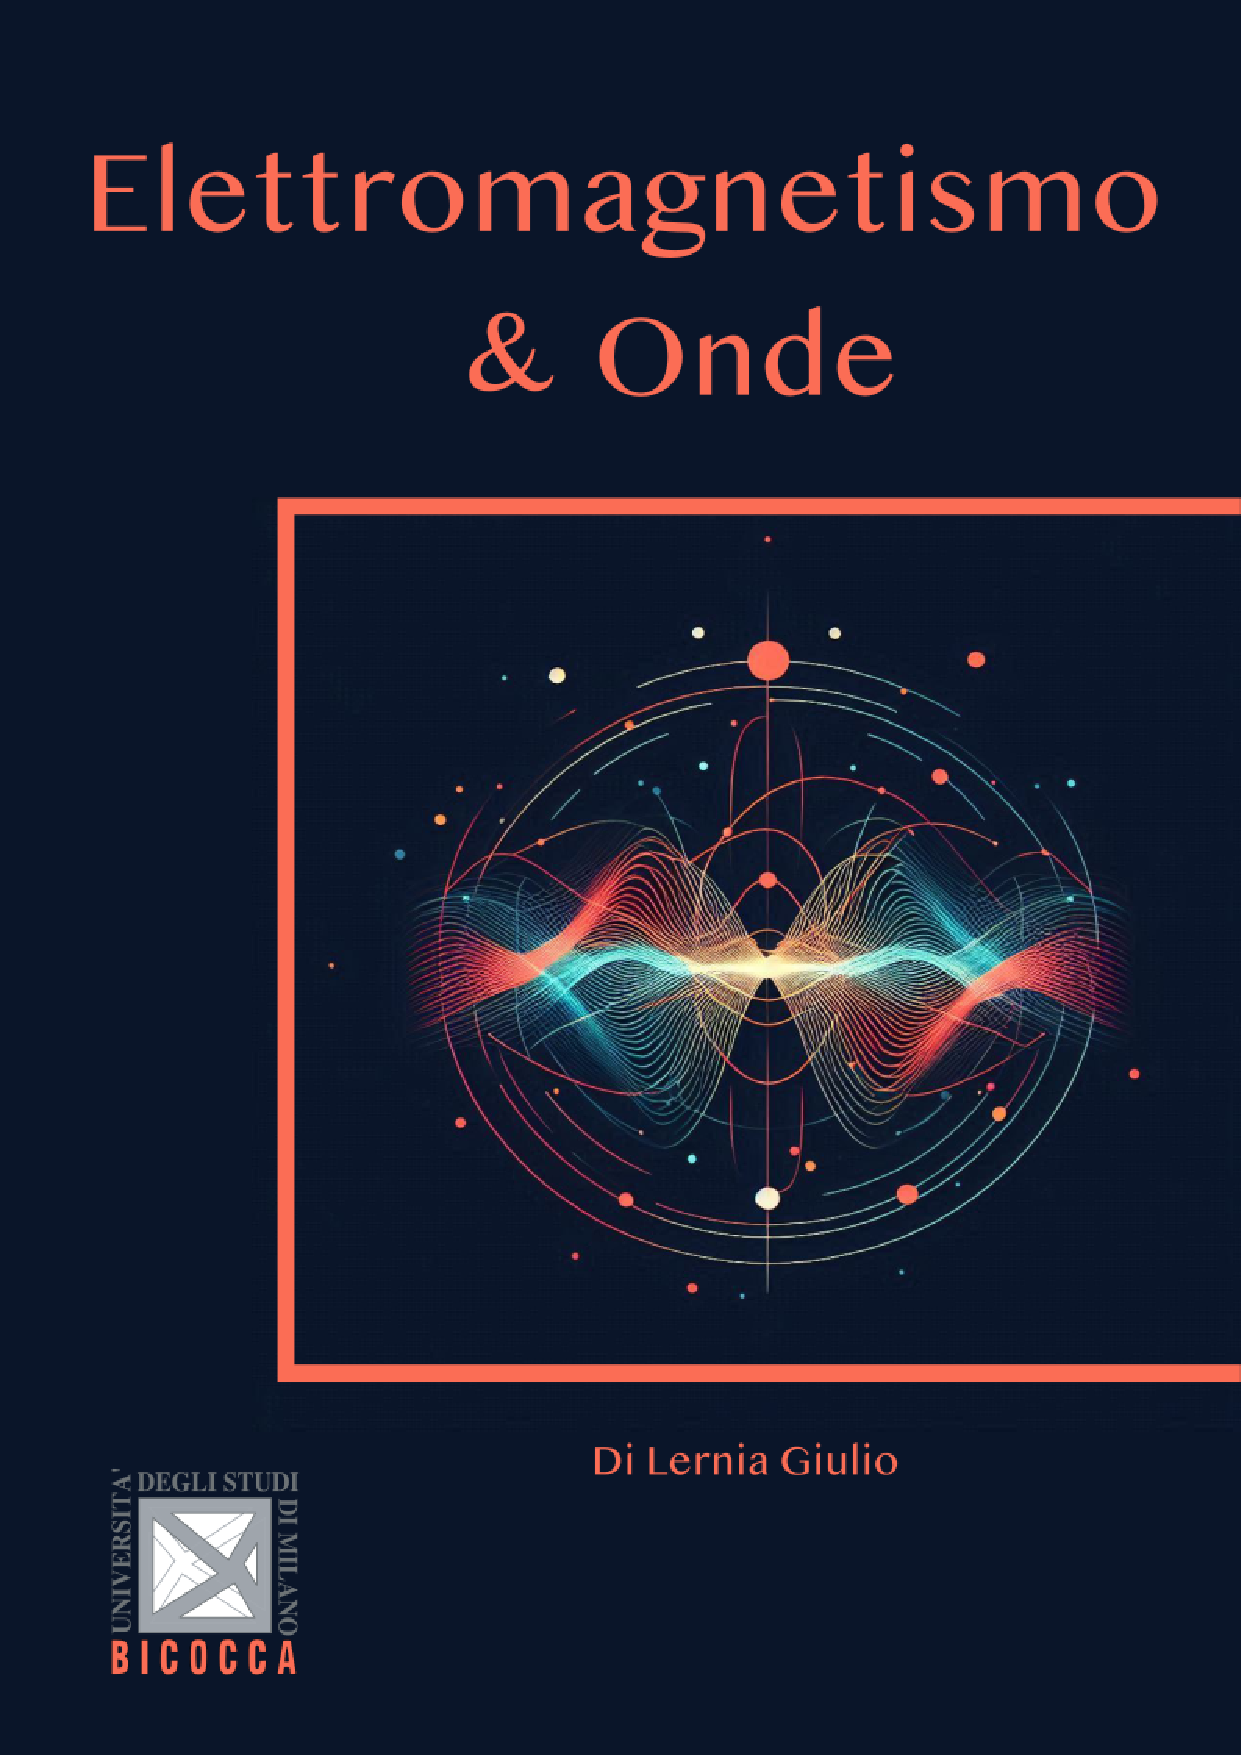
\includepdf{copertina_fisica2.pdf}
	\tableofcontents
	\setcounter{chapter}{-1}
\chapter{Introduzione}


	\setcounter{chapter}{0}
\chapter{Elettrostatica}

\section{Propriet\`a elementari dell'interazione elettrica di due cariche}

L'interazione tra corpi ''elettrizzati" ha diverse propriet\`a irriducibili. Una di queste \`e lo stato di carica di un corpo che \`e definito da due condizioni:
\begin{itemize}
	\item Carica Positiva (Protoni)
	\item Carica Negativa (Elettroni)
\end{itemize}

che permettono di descrivere una forza d'interazione repulsiva o attrattiva. 
\\
Sperimentalmente si osserva che tutti i corpi (o particelle) possiedono carica e che dati due corpi con lo stesso segno di carica si sperimenta una forza repulsiva e per segni opposti attrattiva. Una delle propriet\`a pi\`u importanti \`e la \textit{conservazione della carica}.
\\
La carica totale di un sistema isolato (ovvero che non scambia carica con l'ambiente), \`e definita dalla somma algebrica delle cariche positive e di quelle negative ed \`e costante.
\begin{equation*}
	Q = \sum q^+ + \sum q^- = \text{cost}
\end{equation*} 
La carica non sono \`e conservata per tutti gli osservatori inerziali, ma \`e anche un invariante relativistico, ovvero la carica totale Q non dipende dall'osservatore.
\\
Un altra propriet\`a importante \`e che la carica \`e \textit{quantizzata}, tale propriet\`a ci dice che in un corpo carico, la carica totale \`e un multiplo intero della carica di un elettrone o di un positrone. Al momento non esiste una spiegazione al motivo per cui la carica sia quantizzata e assuma valori continui.
\\
La materia contiene un numero enorme di protoni ed elettroni $\geq 6 \times 10^{23}/mol$. Una piccola differenza di carica renderebbe la materia non neutra, e dunque elettricamente instabile, dunque la materia in natura possiede carica neutra.

\section{Legge di Coulomb (Elettrostatica)}

L'interazione tra due cariche puntiformi e stazionarie, ovvero fisse l'una rispetto all'altra e nel riferimento del laboratorio, \`e descritta dalla legge di forza 
\begin{equation}
	\bold{F} = k \frac{q_1q_2}{r_{12}^2} \;\hat{\mu}_{r_{12}} \quad \text{dove} \quad \vec{r_{12}} = \vec{r_2} - \vec{r_1}
\end{equation}
che esprime la forza esercitata dalla prima carica sulla seconda.
\\
La dipendeza dal prodotto delle cariche fa si che a seconda del loro segno si abbia il verso dell'interazione.
\begin{itemize}
	\item Per una coppia di cariche (+,-) si ha che $\bold{F}$ \`e attrattiva. 
	\item Per una coppia (+,+) o (-,-) si ha che $\bold{F}$ \`e repulsiva.  
\end{itemize}
Il valore della costante k, e della carica, dipende dalla scelta del sistema di misura. Nel sistema internazionale la carica \`e misurata in Coulomb (C) e la costante k \`e posta nella forma 
\begin{equation*}
	k = \frac{1}{4 \pi \varepsilon_0} = 8,81 \times 10^9 \;  \frac{N m^2}{C} \quad \text{e} \quad \varepsilon_0 = 8.85 \times 10^{-12} \; \frac{C^2}{Nm^2} 
\end{equation*}
il termine $\varepsilon_0$ prende il nome di \textit{costante dielettrica nel vuoto} e il suo valore dipende dalle propriet\`a del mezzo rispetto a cui avviene l'interazione elettrostatica, in questo caso stiamo considerando il vuoto.
\\ 
Utilizziamo l'unit\`a di misura dell'Ampere (A) che rappresenta l'intensit\`a di corrente posta tra due fili paralleli posti a un metro di distanza e che generano una forza di $\mu_0 = 4 \pi \times 10^{-7} \; N$. La carica elementare di un elettrone \`e pari a 
\begin{equation*}
	e = - 1.6 \times 10^{-19} \;C
\end{equation*}
che coincide con quella di un protone, ma con segno opposto.
\\
L'interazione di Coulomb coinvolge oggetti che possiedono massa, ma l'interazione gravitazionale tra le cariche elementari \`e trascurabile.
\subsubsection{Esempio}
Se consideriamo l'interazione tra due protoni distanti 1 metro e ricordando che la costante gravitazionale \`e $G = 6.67 \times 10^{-11} \; \frac{m^3}{Kgs^2}$ e la massa di un protone \`e pari a $m_p = 1.67 \times 10^{-27} \; Kg $ si ha che il rapporto tra forza gravitazionale e di Coulomb \`e 
\begin{equation*}
\frac{F_G}{F_{el}} = \frac{Gm_p^2}{kp^2} \approx 10^{-36}
\end{equation*}

\begin{remark}
Tra le cariche elementari si esercita anche una forza magnetica, associata al momento magnetico elementare della particella ( propriet\`a quantistica associata allo SPIN). Su distanze atomiche, ovvero di un $\mathring{A} = 10^{-10} m$, l'interazione magnetica elementare \`e  $\approx 10^4$ volte meno intensa dell'interazione elettrostatica e a livello macroscopico \`e totalmente trascurabile (l'intensit\`a diminuisce come $\frac{1}{r^3}$).
\end{remark}

\section{Principio di Sovrapposizione}

Consideriamo un sistema costituito da tre cariche $q_1,q_2$ e $q_3$, possiamo calcolare la forza di Coulomb esercitata su coppie distinte 
\begin{equation*}
	\begin{aligned}
		& \bold{F}_{13} = \frac{1}{4\pi \varepsilon_0} \frac{q_1q_3}{r_{13}^2}\hat{\mu}_{13} \\[0.3cm]
		& \bold{F}_{12} = \frac{1}{4\pi \varepsilon_0} \frac{q_1q_2}{r_{12}^2}\hat{\mu}_{12} \\[0.3cm]
		& \bold{F}_{23} = \frac{1}{4\pi \varepsilon_0} \frac{q_2q_3}{r_{23}^2}\hat{\mu}_{23} \\
	\end{aligned}
\end{equation*}
Se vogliamo calcolare la forza su una singola carica, per esempio $q_3$, si ha evidenza sperimentale che la forza complessiva su di essa \`e data da 
\begin{equation*}
	\bold{F}_{3} = \frac{1}{4 \pi \varepsilon_0} \frac{q_1q_3}{r_{13}^2}\hat{\mu}_{13} \; + \; \frac{1}{4\pi \varepsilon_0} \frac{q_2q_3}{r_{23}^2}\hat{\mu}_{23}
\end{equation*}
ovvero \`e somma vettoriale delle forze elettrostatiche dovute a tutte le altre cariche nel sistema.


\subsection{Distribuzioni di carica per corpi continui}

\begin{wrapfigure}{r}{0.5\textwidth}
  \begin{center}
    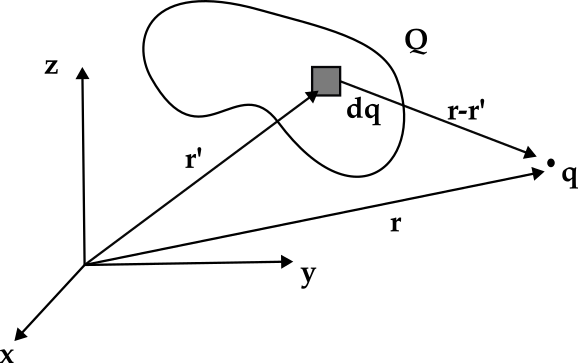
\includegraphics[width=0.4\textwidth]{images/chargeDist}
  \end{center}
\end{wrapfigure}

I sistemi macroscopici sono costituiti da un numero elevato di cariche e tipicamente il suo bilancio \`e neutro, ovvero si ha un egual numero di elettroni e protoni. Quando l'equilibrio viene rotto vengono spostate molte cariche e dunque il problema tipico che viene affrontato \`e quello di determinare la forza esercitata da una distribuzione di carica generica. Per farlo ricorriamo al principio di sovrapposizione. 
\\

\noindent Se consideriamo una carica q interagente con una porzione di carica dq infinitesima di una distribuzione continua Q, abbiamo che la forma esercitata tra le due cariche \`e data da
\begin{equation*}
	d\bold{F} = \frac{1}{4 \pi \varepsilon_0} \frac{qdq}{|\vec{r} -\vec{r'}|^2}\hat{\mu}_{rr'}
\end{equation*}
la forza d'interazione complessiva sar\`a data dall'integrale rispetto alla carica totale della distribuzione della forza infinitesima 
\begin{equation*}
	\bold{F} = \frac{1}{4 \pi \varepsilon_0} \int_{Q} \frac{qdq}{|\vec{r} -\vec{r'}|^2}\hat{\mu}_{rr'}
\end{equation*}
posto $dq' = \rho(\vec{r})dV$ definiamo il termine $\rho(\vec{r})$ come desint\`a volumica di carica e possiamo riscrivere la forza di Coulomb rispetto al volume della distribuzione di carica
\begin{equation*}
	\bold{F} = \frac{1}{4 \pi \varepsilon_0} \int_{V} \frac{\rho(\vec{r})dV}{|\vec{r} -\vec{r'}|^2}\hat{\mu}_{rr'}
\end{equation*}

Se l'elemento di carica considerato dal corpo continuo \`e macroscopicamente piccolo, possiamo considerare le densit\`a di carica funzioni continue rispetto la posizione, mentre se \`e microscopicamente grande le densit\`a sono funzioni regolari della posizione. In sostanza nel primo caso il volume infinitesimo dV considerato possiede un grande quantit\`a di cariche e quindi \`e trascurabili la natura corpuscolare delle cariche e quindi possiamo trattarlo come un elemento continuo.

\subsection{Configurazioni Notevoli di carica}
Le distribuzioni carica non assumono solo forme tridimensionali, ma possono essere superficiali o lineari, per entrambi i casi si definiscono:
\subsubsection{Distribuzione superficiale di carica}

Consideriamo uno strato sottile (di spessore trascurabile) di area S di un materiale. Allora avremo che 

\begin{minipage}{0.6\textwidth}
\begin{equation*}
dq = \rho dV = \rho (tdA) = (\rho t)dA = \sigma dA
\end{equation*}
\end{minipage}
\begin{minipage}{0.4\textwidth}
\centering
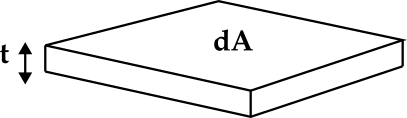
\includegraphics[width=\textwidth]{images/areica.png}
\end{minipage}
dove 
\begin{equation*}
	\sigma = \frac{dq}{dA}
\end{equation*}
prende il nome di \textit{densit\`a di carica areica}. La corrispettiva forza esercita da una superficie di carica \`e data dall'integrale di superficie della forza di Coulomb per una carica sonda q 
\begin{equation*}
	\bold{F} = \int_{S}d\bold{F} = \frac{q}{4 \pi \varepsilon_0} \int_{S} \frac{\sigma(\vec{r})dA}{|\vec{r}-\vec{r'}|^2} \mu_{rr'}
\end{equation*}

\subsection{Distribuzione lineare di carica}

Consideriamo un cavo  la cui sezione ha superficie A, e prendiamone un tratto infinitesimo, allora la quanti\`a di carica contenuta sar\`a data da

\begin{minipage}{0.6\textwidth}
\begin{equation*}
dq = \rho dV = \rho (Adl) = (\rho A)dl = \lambda dl
\end{equation*}
\end{minipage}
\begin{minipage}{0.3\textwidth}
\centering
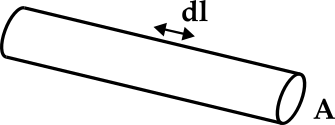
\includegraphics[width=\textwidth]{images/lineica.png}
\end{minipage}
\\
dove 
\begin{equation*}
	\lambda = \frac{dq}{dl}
\end{equation*}
prende il nome di \textit{densit\`a lineica di carica}. Se consideriamo una carica sonda q la forza esercitata dalla carica lineare su tale particella sar\`a espressa dalla legge di Coulomb formulata nel seguente modo
\begin{equation*}
	\bold{F} = \int_{L} d\bold{F} = \frac{q}{4 \pi \varepsilon_0} \int_{L} \frac{\lambda(\vec{r'})dl}{|\vec{r} - \vec{r'}|^2} \hat{\mu}_{rr'}
\end{equation*}

\section{Energia di un Sistema di Cariche}

In linea di principio, tutta l'elettorstatica \`e compresa nella legge di Coulomb. Date le cariche e le loro posizioni possiamo ricavare tutte le forze elettriche agenti, o nel caso in cui queste siano in moto per azione di altre forze possiamo determinare la condizione di equilibrio elettrostatica.
\\
Come fattoper la meccanica introduciamo il concetto di energia per l'elettromagnetismo, il che \`e assume un aspetto molto importante dato che le forze elettriche sono di natura \textit{conservativa}.
\\

\noindent Consideriamo un sistema formato da due particelle che inizialmente si trovano ad una grande distanza e dotate di carica $q_1$ e $q_2$. Se ora vogliamo avvicinarle tra loro ad una distanza $\bold{r}_{12}$ quanto lavoro dobbiamo compiere ?
\\
Per rispondere a questa domanda utilizziamo la generica definizione di lavoro, ovvero che il lavoro compiuto in un sistema \`e dato dall'integrale di linea della forza agente sulle cariche.
\begin{equation*}
	W = \int \bold{F} \cdot d\bold{r}
\end{equation*}
dove nel caso di cariche la forza agente \`e per spostare una carica verso l'altra ha la stessa intensit\`a di quella di Coulomb, ma con verso opposto.
\begin{equation}
	W = -\frac{1}{4 \pi \varepsilon_0} \int _{\infty}^{\bold{r}_{12}}\frac{q_1q_2}{\bold{r}^2}d\bold{r} = \frac{1}{4 \pi \varepsilon_0} \frac{q_1q_2}{r_{12}}
\end{equation} 
Di conseguenza abbiamo che il lavoro compiuto sul sistema \`e:
\begin{itemize}
	\item $W > 0$ per cariche dello stesso segno.
	\item $W < 0$ per cariche di segno opposto.
 \end{itemize}
 Dato che la forza \`e conservativa si ha che il lavoro compiuto non dipende dal percorso scelto per avvicinare le due cariche, ma solo dalla posizione iniziale e finale.
 \\
 
 \noindent Supponiamo di introdurre una terza carica $q_3$ all'interno del sistema e di portarla da un punto molto lontano al punto $P_3$ che si trova  a distanza $r_{31}$ per la prima carica e $r_{21}$ per la seconda carica. Il lavoro richiesto per compiere tale operazione \`e 
 \begin{equation*}
 	W_3 = - \int_{\infty}^{P_3}\bold{F}_3 \cdot d\bold{r}
 \end{equation*} 
 Grazie al principio di sovrapposizione abbiamo che la forza totale agente sulla carica $q_3$ \`e data da 
 \begin{equation*}
 	W_3 = - \int (\bold{F}_{31}+\bold{F}_{32}) \cdot d\bold{r} = - \int \bold{F}_{31} \cdot d\bold{r} - \int \bold{F}_{32} \cdot d \bold{r}
 \end{equation*}
 ovvero il lavoro che si compie per portare $q_3$ in $P_3$ \`e la somma del lavoro necessario quando \`e presente solo $q_1$ e di quello necessario quando \`e presente solo $q_2$. Dal risultato ottenuto in (1.2) si ha che
 \begin{equation*}
 	W_3 = \frac{1}{4 \pi \varepsilon_0} \left (\frac{q_1q_3}{r_{31}} + \frac{q_2q_3}{r_{32}} \right )
 \end{equation*}
 Il lavoro totale compiuto per realizzare la distribuzione di tre cariche, che indicheremo con U, \`e 
 \begin{equation}
 	U = W +W_3 = \frac{1}{4 \pi \varepsilon_0} \left (\frac{q_1q_2}{r_{12}} + \frac{q_1q_3}{r_{31}} + \frac{q_2q_3}{r_{32}} \right)
 \end{equation}
 Notare che l'espressione \`e simmetrica rispetto a $q_1,q_2$ e $q_3$ e dunque \`e indipendente da quale carica si considera d'introdurre per ultima. Dunque U non dipende dall'ordine delle cariche con cui si assembla il sistema e non dipende dal percorso che si sceglie per farlo, l'energia totale del sistema dipende unicamente dalla posizione iniziale e finale, come ci si aspetterebbe da un sistema le cui forze agenti sono conservative.
 \\
 Possiamo definire U come \textit{energia potenziale elettrica} del sistema. Quando si definisce un energia potenziale in un sistema vi \`e una certa arbitrariet\`a nella scelta nella sua definizione, in questo caso si \`e scelto come zero di U la configurazione in cui le tre cariche si trovano ad una distanza cos\`i grande tra loro che non vi \`e interazione tra di esse.
 \\
 
 \noindent \`E semplice la generalizzazione del risultato (1.3) ad un sistema costituito da N particelle, \`e sufficiente considerare il lavoro della forza su coppie distinte e sommarlo.
 \begin{equation}
 	U = \frac{1}{2} \sum_{j=1}^N \sum_{k \neq j} \frac{q_jq_k}{r_{jk}}
 \end{equation}
 Il fattore $1/2$ serve ad eliminare i conteggi doppi del lavoro dato che le coppie con ordine (j,k) e (k,j) restituiscono il medesimo risultato e dunque si sommano.

\begin{remark}\
\begin{itemize}
\item 	Se $q_1$ e $q_2$ sono concordi in segno: $U(r) > 0$ le cariche (se non vincolate) si allontanano e l'energia potenziale diminuisce a favore dell'energia cinetica.
\item Se $q_1$ e $q_2$ sono discordi in segno: $U(r) < 0$ le cariche si avvicinano e l'energia potenziale aumenta a sfavore dell'energia cinetica.
\end{itemize}
\end{remark}
\noindent Un sistema le cui cariche a coppie hanno $U(r) < 0$ \`e legato  e occorre compiere del lavoro per separare le cariche. L'energia potenziale per un sistema di questo tipo viene denominata \textit{energia di legame}.

\subsubsection{Esempio - Separazione di una molecola di sale}

Consideriamo la molecola di sale data da $Na^+Cl^-$ costituita da un atomo di sodio (Na) e di cloro (Cl) poste ad una distanza $d \approx 3 \mathring{A}$. Quando l'atomo di sodio e cloro vengono separate a una distanza $r$ molto grande il sistema \`e ben descritto da due cariche puntiformi con carica $|q| = e$. L'energia potenziale (o di legame in questo caso) del sistema \`e data da 
\begin{equation*}
	U (d) = - \frac{e^2}{4 \pi \varepsilon_0 d} \approx - 7.7 \times 10^{-19}J 
\end{equation*}
Se consideriamo un sistema di particelle che pu\`o essere messo in agitazione termica l'energia termica \`e approssimativamente di $\frac{5}{2}kT  = 10^{-20} J$ per una temperatura $T = 300 \;K$. L'energia fornita termicamente \`e di quasi due volte inferiore all'energia necessaria per separare il sodio dal cloro.

\section{Campo Elettrico}

Supponiamo di avere una distribuzione di cariche $q_1,q_2,...,q_n$ fisse rispetto ad un osservatore e di volerne studiare l'interazione con una carica $q_0$. Trascurando la forza d'interazione tra le cariche e considerando solo la forza di Coulomb complessiva sulla nostra carica sonda $q_0$ si ha che 
\begin{equation*}
	\bold{F}_{0} = \sum_{j=1}^N \frac{1}{4 \pi \varepsilon_0}\frac{q_0q_j}{r_{0j}^2}\hat{\mu}_{0j}
\end{equation*}
dove $\bold{r}_{0j}$ \`e la posizione delle cariche rispetto alla posizione di $q_0$. La risultante delle forze risulta essere proporzionale alla carica della particella sonda, se dividiamo per questa quantit\`a la forza totale, otteniamo una grandezza vettoriale che dipende unicamente dalla struttura del sistema iniziale di cariche $q_1,...,q_n$ e dalla posizione della carica $q_0$. Il vettore cos\`i definito prende il nome di \textit{campo elettrico} associato alle cariche $q_1,...q_n$ e viene definito nel seguente modo
\begin{equation}
	\bold{E}(x,y,z) = \frac{\bold{F}_{0}}{q_0} = \frac{1}{4 \pi \varepsilon_0}\sum_{j=1}^N \frac{q_j}{r_{0j}^2}\hat{\mu}_j
\end{equation}
Definito un campo elettrico per qualsiasi carica q, la forza dovuta alla distribuzione di cariche (che abbiamo supposto stazionarie) \`e esprimibile tramite 
\begin{equation*}
	\bold{F}_{q} = q \bold{E}
\end{equation*}
Il campo elettrico associa a ogni punto in un sistema una propriet\`a locale, se conoscia il valore di $\bold{E}$ in una piccola regione, senza bisogno di ulteriori informazioni, conosciamo cosa accadr\`a a qualsiasi carica posta in quella zona, senza necessariamente conoscere come siano distribuite le cariche sorgente.

\subsection{Rappresentazione del Campo Elettrico}

Per visualizzare un campo elettrico \`e necessario associate un vettore, cio\`e, intensit\`a, verso e direzione in ogni punto dello spazio. Inazittuto si consideri il fatto che per per una carica puntiforme la simmetria del campo \`e sferica e la sua direzione \`e data dal segno della carica. Data la simmetria del campo, visto che darne una rappresentazione tridimensionale diventa complicato, possiamo sfruttare tale propriet\`a per darne una raffigurazione bi-dimensionale, che non ne rende inefficacie la descrizione fisica.
\\

\noindent Consideriamo il campo generato da una carica Q positiva (e negativa), e iportizziamo di testarlo con una carica $q_0$, in questo vaso avremo che il campo percepito dalla carica sonda \`e lungo la congiungente e quindi \`e espresso come
\begin{equation*}
	\bold{E}(x,y) = \frac{1}{4 \pi \varepsilon_0} \;
	\frac{Q}{r_0^2} \;\hat{\mu}_{r_0} 
\end{equation*} 
vogliamo riscrivere il campo rispetto alla base di vettori $\{e_1,e_2\}$ che definiscono un sistema ortonormale.

 
\begin{figure}[!ht]
\vspace{0.2in}
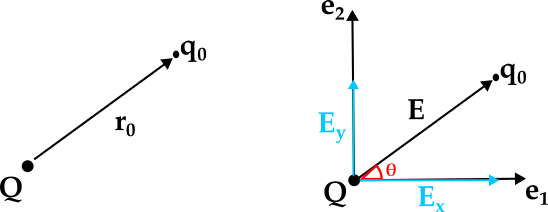
\includegraphics[width= 8cm]{images/decomp}	
\centering
\vspace{0.1in}
\end{figure}
prendendo la posizione di Q come origine del sistema riscriviamo la lunghezza radiale in coordinate cartesiane $r_0^2 = x^2 + y^2$. Le proiezioni del campo rispetto agli elementi della base sono date da 
\begin{equation*}
	\left \{ \begin{array}{l}
		E_x = E \cos\theta \\
		E_y = E \sin\theta 
	\end{array}\right.
\end{equation*}
utilizzando le relazioni fondamentali della tringonometria dove $\cos\theta = \frac{x}{x^2+y^2}$ e $\sin\theta = \frac{y}{x^2+y^2}$ le componenti del campo vettoriale si riscrivono come
\begin{equation*}
	\left \{ \begin{array}{l}
		E_x(x,y) = E  \frac{x}{x^2+y^2} = \frac{Q}{4 \pi \varepsilon_0} \; \frac{x}{(x^2+y^2)^{3/2}}\\
		E_y(x,y) = E \frac{y}{x^2+y^2}  = \frac{Q}{4 \pi \varepsilon_0} \; \frac{y}{(x^2+y^2)^{3/2}}
	\end{array}\right.
\end{equation*}
Conoscendo il valore delle componenti in ogni punto del piano, possiamo definirne direzione, verso e intensit\`a del campo vettoriale. 
\begin{figure}[!ht]
\centering
\begin{minipage}{0.4\textwidth}
  \centering
  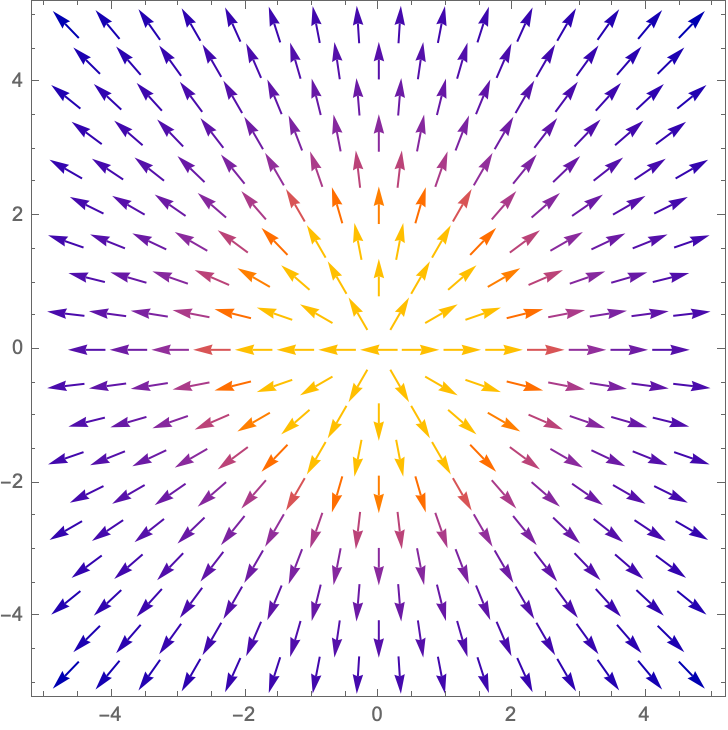
\includegraphics[width=0.8\linewidth]{images/positive}
  \captionof{figure}{Campo Elettrostatico per una sorgente di carica positiva}
\end{minipage}%
\hspace{0.8cm}
\begin{minipage}{0.4\textwidth}
  \centering
  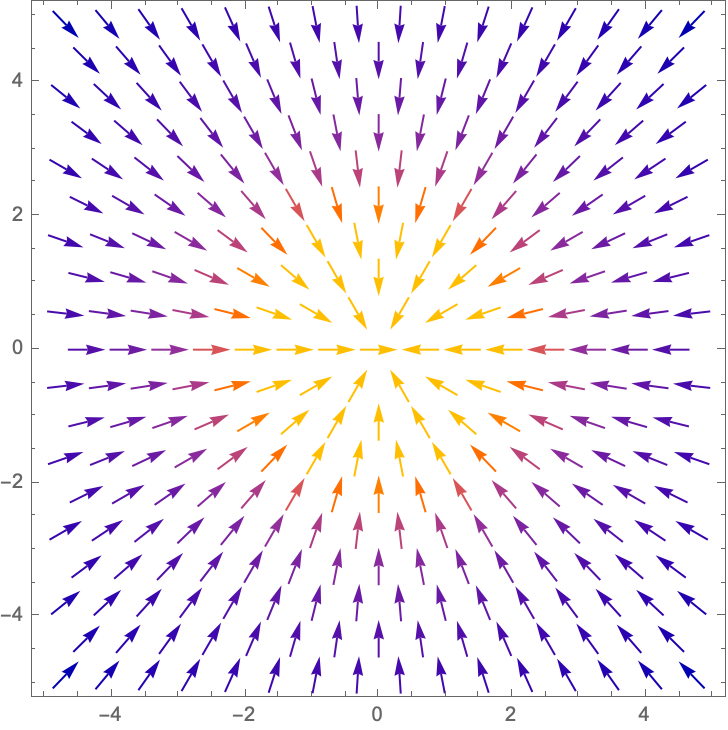
\includegraphics[width=0.8\linewidth]{images/negative}
  \captionof{figure}{Campo Elettrostatico per una sorgente di carica negativa}
\end{minipage}
\end{figure}
 Dalle figura si nota come l'intensit\`a del campo decresca come $\frac{1}{r^2}$ e dunque risultando pi\`u intenso in prossimit\`a della sorgente.
 \\
 \begin{lstlisting}[language = Mathematica]
Mathematica Snippet 

Q = 1.6*10^(-19)
d = 8.854187822*10^(-12)

Ex[q_, x_, y_, x0_, y0_] := 
 q/(4*Pi*d)*((x - x0)/((x - x0)^2 + (y - y0)^2)^(1.5))

Ey[q_, x_, y_, x0_, y0_] := 
 q/(4*Pi*d)*((y - y0)/((x - x0)^2 + (y - y0)^2)^(1.5))

{VectorPlot[{Ex[Q, x, y, 0, 0], Ey[Q, x, y, 0, 0]}, {x, -5, 
   5}, {y, -5, 5}], 
 VectorPlot[{Ex[-Q, x, y, 0, 0], Ey[-Q, x, y, 0, 0]}, {x, -5, 
   5}, {y, -5, 5}]} 
 \end{lstlisting}
 
Dato che il campo elettrico gode del principio di sovrapposizione si ha che per configurazioni di pi\`u cariche si applica lo stesso metodo, sommando le componenti dei campi elettrici generato dalle singole cariche in tutti i punti dello spazio.
\begin{figure}[!ht]
\vspace{0.1in}
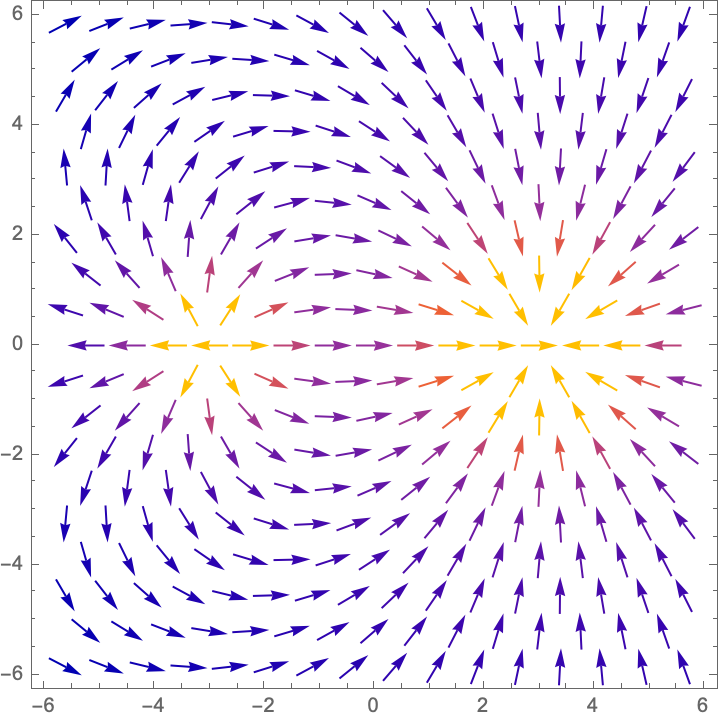
\includegraphics[width = 7cm]{images/interac}	
\centering
\vspace{0.1in}
\caption{Campo generato da una carica Q in (-3,0) e una carica -3Q posta in (3,0)}
\end{figure}

\newpage 
 
\begin{lstlisting}[language = Mathematica]
Mathematica Snippet 

Exx[q1_, q2_, x_, y_, x0_, y0_, x1_, y1_] =  
	Ex[q1, x, y, x0, y0] + Ex[q2, x, y, x1, y1]

Eyy[q1_, q2_, x_, y_, x0_, y0_, x1_, y1_]  = 
	Ey[q1, x, y, x0, y0] + Ey[q2, x, y, x1, y1]

VectorPlot[
{Exx[Q, -3*Q, x, y, -3, 0, 3, 0], Eyy[Q, -3*Q, x, y, -3, 0, 3, 0]}, 
{x, -6, 6}, {y, -6, 6}
]
\end{lstlisting}
Un altro modo per rappresentare un campo, e in questo caso un campo elettrico, \`e utilizzando le linee di flusso (forza). Queste si ottengono risolvendo il sistema di equazioni differenziali 
\begin{equation*}
\left \{\begin{array}{l}
	\frac{dx}{dt}= E_x(x,y)\\
	\frac{dy}{dt} = E_y(x,y)
	\end{array}\right.
\end{equation*}
dove il campo elettrico risulta essere tangente alle soluzioni (x(t),y(t)) di questo sistema. (x,y) descrivono curve regolari e continue, tranne che nei punti di singolarit\`a o nei punti dove il campo \`e nullo. Graficamente l'informazione d'intensit\`a di un campo viene recuperata dal fatto che le linee di forza si addensano in prossimit\`a delle cariche sorgente dove il campo \`e intenso e diventano rarefatte allontanandosi.

 
\begin{figure}[!ht]
\vspace{0.1in}
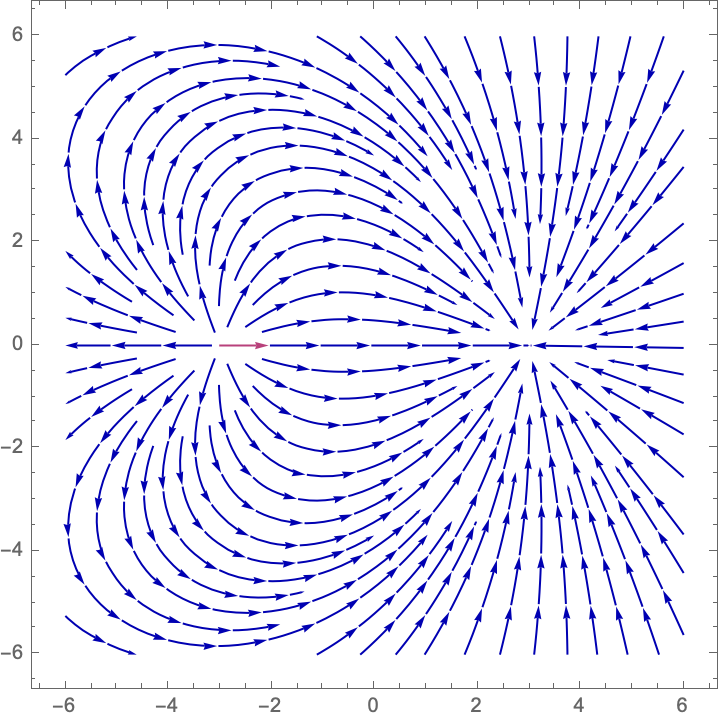
\includegraphics[width = 6cm]{images/stream}	
\centering
\vspace{0.1in}
\caption{Linee di Forza associate per una carica Q in (-3,0) e -3Q in (3,0)}
\end{figure}

\newpage

\begin{lstlisting}[language = mathematica]
Mathematica Snippet 

Exx[q1_, q2_, x_, y_, x0_, y0_, x1_, y1_] = 
	Ex[q1, x, y, x0, y0] + Ex[q2, x, y, x1, y1]
Eyy[q1_, q2_, x_, y_, x0_, y0_, x1_, y1_]  = 
	Ey[q1, x, y, x0, y0] + Ey[q2, x, y, x1, y1]

StreamPlot[
{Exx[Q, -3*Q, x, y, -3, 0, 3, 0], 
  Eyy[Q, -3*Q, x, y, -3, 0, 3, 0]}, 
  {x, -6, 6}, {y, -6, 6}
  ]
\end{lstlisting}

\section{Flusso di un Campo Vettoriale}

La relazione tra campo elettrico e sorgenti pu\`o essere espressa in forma semplice e utile tramite la nozione di \textit{flusso} del campo elettrico attraverso una superficie.

\begin{wrapfigure}{l}{0.4\textwidth}  % "r" means to wrap on the right, width of the figure box
    \centering
    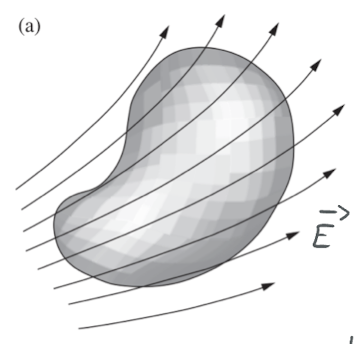
\includegraphics[width=0.25\textwidth]{images/flux}  % Adjust the width as needed
\end{wrapfigure}
\vspace{0.5cm}
\noindent Si immagini di avere una superficie chiusa come in figura in una regione di spazio in cui \`e presente un campo elettrico $\bold{E}(x,y,z)$ generato da una distribuzione di cariche. 

Procediamo con l'affettare tale superficie in piccoli elementi di area $\Delta A_j$ e al centro di ciascuno di essi applichiamo un vettore ortogonale alla superficie la cui intensit\`a \`e data dall'area dell'elemento. Definendo $\bold{\Delta A}_j = \Delta A_j\hat{n}$
dove $\hat{n}$ \`e un versore ortogonale alla superficie considerata e con direzione uscente.

\begin{wrapfigure}{r}{0.4\textwidth}  % "r" means to wrap on the right, width of the figure box
    \centering
    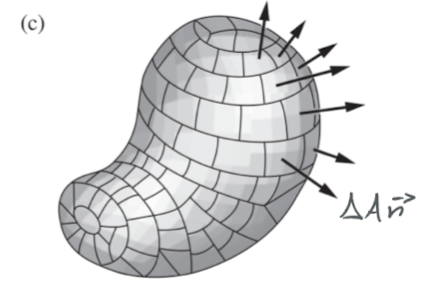
\includegraphics[width=0.3\textwidth]{images/divide}  % Adjust the width as needed
\end{wrapfigure}
Se l'area della porzione di superficie \`e sufficientemente piccola, in quella regione di spazio possiamo considerare il campo elettrico $\bold{E}(x,y,z)$ costante. 
\\

\noindent  Definiamo il flusso del campo elettrico rispetto all'area $\Delta A_j$ come la sua proiezione lungo la direzione del vettore d'area. 
\begin{equation}
	\phi_j = \bold{E} \cdot \bold{\Delta A}_j 
\end{equation} 
Tale definizione prende ispirazione della fluido dinamica dove tale grandezza definisce la rapidit\`a con cui fluisce  il campo elettrico  alla superficie orientata. Infatti se consideriamo un fluido  con velocit\`a $\bold{v}$ in regime stazionario si ha che la portata \`e data da  
\begin{equation*}
	d\phi = \bold{v} \cdot \bold{\Delta A} = \frac{dV}{dt}
\end{equation*} 
Il prodotto scalare recupera ci definisce la proiezione del campo lungo la direzione ortogonale alla superficie, ovvero la superficie efficace attraverso cui fluisce il campo.
 
\begin{figure}[!ht]
\vspace{0.1in}
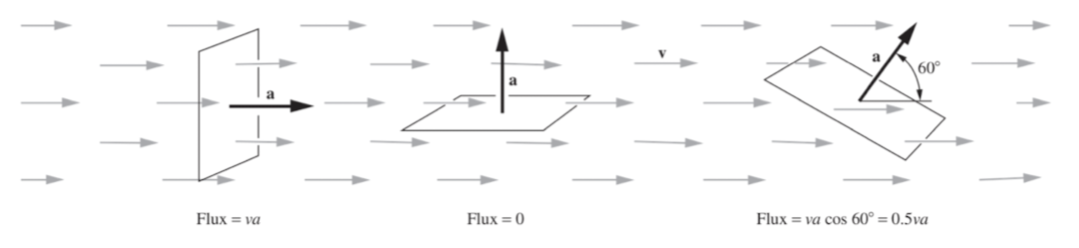
\includegraphics[width = 15.5cm]{images/orient}	
\centering
\vspace{0.1in}
\end{figure}
La definizione di flusso \`e applicabile a qualsiasi funzione vettoriale, indipendentemente dalla variabile fisica che rappresenta.
\\
Il flusso complessivo attravero la superficie \`e ottenuto sommando i singoli contributi
\begin{equation*}
	\begin{aligned}
		& \phi(\bold{E}) = \sum_{j} \bold{E}\cdot \bold{\Delta A}_{j} \quad \text{(Caso Discreto)} & \\[0.5cm]
		& \phi(\bold{E}) = \int_{S}\bold{E} \cdot \bold{dA} \quad \text{(Limite Continuo)}
	\end{aligned}
\end{equation*}

\begin{remark}	
\end{remark}

Notare che, il flusso \`e una funzione che preso un vettore gli associa uno scalare 
\begin{equation*}
	\phi : \mathbb{R}^3 \to \mathbb{R}
\end{equation*}
e inoltre restituisce informazioni sull'insieme del sistema e non locali.

\section{Legge di Gauss}

Consideriamo una regione chiusa dello spazio $ V \subset \mathbb{R}^3$ e consideriamo $S = \partial V$ la superficie di V.  Ipotizziamo che sia presente una distribuzione di carica continua (o discreta) all'interno della regione V, avremo che il flusso del campo elettrico generato attraverso la superficie S \`e dato da 
\begin{equation*}
\begin{aligned}
	& \phi(\bold{E}) = \int_{S} \bold{E} \cdot d\bold{A} = \frac{1}{\varepsilon_0}\int_{V} \rho(\bold{r})dV \quad \text{(Distribuzioni Continue)} & \\[0.5cm]
	& \phi(\bold{E}) = \int_{S} \bold{E} \cdot d \bold{A} = \frac{1}{\varepsilon_0} \sum_{i}q_i
	\quad \text{(Distribuzioni Discrete)}
\end{aligned}
\end{equation*}
Tale relazione prende il nome di \textit{legge di Gauss}. I termini di destra coincidono la quantit\`a di carica complessiva contenuta all'interno della regione V, infatti possiamo definire
\begin{equation*}
	Q = \int_{V} \rho(\bold{r})dV
\end{equation*} 
Con questa legge noto il campo vettoriale ( quindi intensit\`a e geometria) \`e possibile risalire alla carica complessiva delle sorgenti.
\\

\noindent Notare che la forma della \textit{superficie Gaussiana} S non influenza il risultato della Legge di Gauss fin tanto che la carica resta all'interno del volume della regione di spazio V. In sostanza l'integrale del flusso non dipende dalla geometria della superficie, ma dipende dalla sua topologia.
\begin{proof}
	Dimostriamo la non dipendenza della legge di Gauss dalla forma della superficie.
	\\
	I) Consideriamo il campo elettrico dato da una carica puntiforme 
	\begin{equation*}
		\bold{E} = \frac{1}{4 \pi \varepsilon_0} \frac{q}{r^2} \hat{\mu}_{r}
	\end{equation*}
	e che la carica sia racchiusa all'interno di una sfera di raggio R, il flusso attraverso di essa \`e dato da 
	\begin{equation*}
		\phi(\bold{E}) = \int_{S} \bold{E} \cdot d\bold{A} = E(R^2) \int_{S}dA = \frac{1}{4 \pi \varepsilon_0} \frac{q}{R^2} (4\pi R^2) = \frac{q}{\varepsilon_0}
	\end{equation*}
	II) Ora poniamo la regione di spazio sferica in un volume generico V chiuso che la contiene, proiettiamo l'elemento di volume dA della superficie sferica su quella generica V, ottenendo un angolo solido 
	\begin{equation*}
		\Omega = \frac{dA}{R^2} = \frac{da\cos\theta}{r^2}
	\end{equation*}
	 
\begin{figure}[!ht]
\vspace{0.1in}
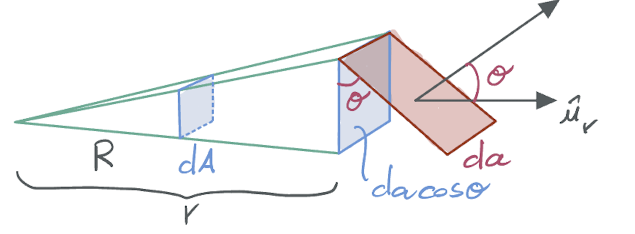
\includegraphics[width = 9cm]{images/solid}	
\centering
\vspace{0.1in}
\end{figure} 
dunque l'area infinitesima della superficie esterna V \`e dara da 
\begin{equation*}
	da = dA\frac{r^2}{R^2 \cos \theta }
\end{equation*}
il campo ha simmetria sferica dunque ha direzione radiale $\hat{\mu}_r$ di conseguenza il flusso attraverso la superficie "da" \`e dato da 
\begin{equation*}
	\phi(\bold{E})_{da} = \bold{E}(\bold{r}) \cdot d\bold{a} = E(r)da \cos \theta = E(R)dA = \phi(\bold{E})_{dA}
\end{equation*}
sommando i contributi infinitesimi si ha che 
\begin{equation*}
	\phi(\bold{E})_{V} = \phi(\bold{E})_{S} = \frac{q}{\varepsilon_0}
\end{equation*}	
\end{proof}
\noindent La legge di Gauss \`e verificata per una qualsiasi distribuzione di carica, se ipotiziamo di avere $q_1,...,q_n$ cariche in una regione chiusa di spazio V si ha che per il principio di sovrapposizione il campo elettrico totale \`e dato da 

\begin{equation*}
	\bold{E} = \sum_{i}\bold{E}_{i}
\end{equation*}
dunque il flusso \`e esprimibile come
\begin{equation*}
	\phi(\bold{E}) = \int_{S} \sum_{i} \bold{E}_i \cdot d\bold{a} = \sum_{i} \phi_i(\bold{E}) = \frac{\sum_{i}q_i}{\varepsilon_0}
\end{equation*}

\begin{prop}
	Se $\bold{F} \not\sim  \frac{1}{r^2}$ la legge di Gauss non \`e valida (La legge di Gauss vale anche per la forza gravitazionale)
\end{prop}
\noindent Si ha che $\phi(\bold{E})_V = 0$ per un campo vettoriale $\bold{E}$ in una regione di spazio chiusa V,  se non ci sono cariche interne oppure se il flusso di cariche esterne alla superficie \`e nullo.
\begin{remark}
Dire che $\phi(\bold{E}) = 0 $ non vuol dire necessariamente che $\bold{E} = 0$.	
\end{remark}
\begin{prop}
\noindent Dato il flusso di un campo vettoriale $\bold{E}$  questo \`e il medesimo per tutte le superfici aperte che sottendono lo stesso angolo solido (e sono dalla stessa parte rispetto alla sorgente del campo elettrico). In sostanza \`e sempre possibile calcolare il flusso attraverso una superficie equivalente che semplifica il calcolo.
\end{prop}

\begin{proof}
	 
\begin{figure}[!ht]
\vspace{0.1in}
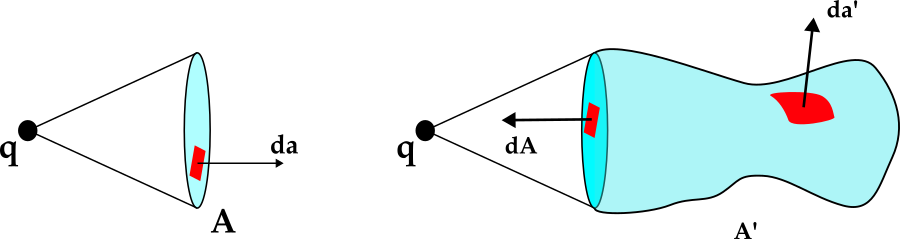
\includegraphics[width = 12cm]{images/same}	
\centering
\vspace{0.1in}
\end{figure}
Consideriamo la superficie chiusa S = A + A', questa non contiene la sorgente di campo "q" e di conseguenza il flusso $\phi_{S}(\bold{E}) = 0$. Se riscriviamo il flusso come
\begin{equation*}
	\phi_S(\bold{E}) = \int_{S = A+A'} \bold{E} \cdot d\bold{A} = \int_{A} \bold{E} \cdot d\bold{A} - \int_{A'} \bold{E} \cdot d\bold{a} = 0
\end{equation*}
dunque si ha che $\phi_{A}(\bold{E}) = \phi_{A'}(\bold{E})$. Il segno negativo compare perch\`e per una superficie chiusa il vettore d'area ha sempre verso uscente rispetto alla superficie)

\end{proof}
\newpage

\subsection{Distribuzione di Carica a Simmetria Sferica}

Consideriamo una distribuzione di carica sferica $\rho$ e di raggio R, all'esterno di essa possiamo approssimare il suo campo a quello di una carica puntiforme, ma come \`e fatto al suo interno? dipende dalla sua distribuzione. Se consideriamo una distribuzione uniforme la carica complessiva \`e data da 
\begin{equation*}
	Q = \frac{4 \pi}{3}R^3 \rho
\end{equation*} 

\begin{wrapfigure}{r}{0.25\textwidth}  % "r" means to wrap on the right, width of the figure box
    \centering
    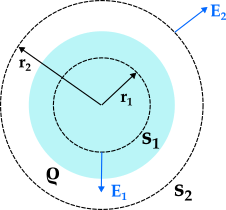
\includegraphics[width=0.3\textwidth]{images/spheric}  % Adjust the width as needed
\end{wrapfigure}

\noindent Consideriamo la superficie sferica S1 come in figura, con centro nell'origine, e raggio $r_1 < R$, la carica contenuta all'interno sar\`a data da 
\begin{equation*}
	Q_{int} = \int_{V}dV\; \rho = \int_{0}^{r_1}dr \; r^2 \int_{0}^{2\pi}d \theta \int_{0}^{\pi}d\varphi \; \sin \varphi = \frac{4 \pi}{3}\rho \; r_1^3 
\end{equation*}
Applicando la legge di Gauss abbiamo che 
\begin{equation*}
\phi(\bold{E}) = \int_{S_1} \bold{E} \cdot d\bold{a}  =	\frac{4 \pi}{3}\rho \; r_1^3 
\end{equation*}
e dunque il campo elettrico sulla superficie $S_1$ \`e data da
\begin{equation*}
	\bold{E}(r_1) = \frac{\rho \; r_1}{3 \varepsilon_0} \hat{\mu}_{r} \quad r_1 \leq R
\end{equation*}

\begin{wrapfigure}{l}{0.4\textwidth}  % "r" means to wrap on the right, width of the figure box
    \centering
    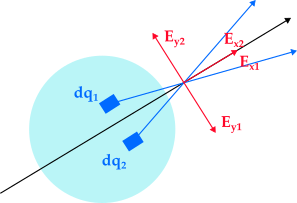
\includegraphics[width=0.4\textwidth]{images/sym}  % Adjust the width as needed
\end{wrapfigure}

L'informazione sulla direzione radiale del campo $\hat{\mu}_{r}$ \`e facilmente recuperabile osservando la simmetria del problema. Consideriamo un sistema di riferimento che divida in due parti simmetriche la sfera, se consideriamo due porzioni di carica $dq_1$ e $dq_2$ su di essa  e li facciamo interagire con una carica sonda $q_0$,posta in un punto che rende equidistanti le cariche, avremo che il campo $\bold{E}$ ha direzione lungo la congiungente $\hat{\mu}_{r0}$ decomponendo rispetto al sistema di riferimento le componenti angolari si eliminato, avendo segni opposti e pari intesit\`a
\begin{equation*}
	E_{y2} + E_{y1} =0
\end{equation*}
e restano solo quelle della componente radiale che si sommano
\begin{equation*}
	\sum_{i}E_{xi} = R_{x}
\end{equation*}
dunque possiamo concludere che il campo abbia direzione radiale.

\begin{wrapfigure}{r}{0.4\textwidth}  % "r" means to wrap on the right, width of the figure box
    \centering
    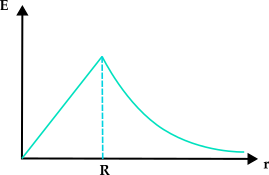
\includegraphics[width=0.4\textwidth]{images/gsphera}  % Adjust the width as needed
\end{wrapfigure}
\vspace{0.5cm}
\noindent Possiamo riassumere i risultati ottenuti per la variazione d'intensit\`a del campo in funzione della posizione radiale, nel seguente modo

\begin{equation}
	\bold{E}(r) = \left \{ \begin{array}{l}
	\frac{Q}{4 \pi \varepsilon_0}\frac{1}{r^2} \hat{\mu}_{r} \quad r >R \\[0.5cm]
	\frac{\rho \; r}{3 \varepsilon_0} \hat{\mu}_{r} \quad r \leq R
	\end{array}\right.
\end{equation}
\newline

\noindent Osserviamo che il campo elettrico \`e continuo in $r=R$, ma la derivata prima $\frac{dE}{dr}$ no, come si osserva dal grafico.

\subsection{Distribuzione di carica a Simmetria Cilindrica (Filo "infinito")}

\begin{wrapfigure}{r}{0.4\textwidth}  % "r" means to wrap on the right, width of the figure box
    \centering
    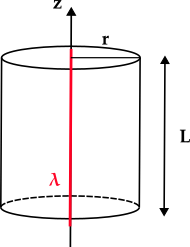
\includegraphics[width=0.25\textwidth]{images/wire}  % Adjust the width as needed
\end{wrapfigure}

Consideriamo una distribuzione di carica lineica $\lambda$ con estensione infinita lungo la direzione z. Attorno ad essa definiamo una superficie Gaussiana cilindrica di raggio $r$ e lunghezza L. La quantit\`a di carica racchiusa sar\`a dara da 
\begin{equation*}
	Q = \frac{\lambda L }{\varepsilon_0}
\end{equation*}
Per ragioni di simmetria il campo elettrico ha simmetria radiale $\hat{\mu}_{r}$. Questo vuol dire che le due basi del cilindro non contribuiscono all'integrale di flusso dato che $\bold{\hat{z}} \cdot \bold{\hat{r}} = 0$. Dunque applicando la legge di Gauss si ha che 
\begin{equation*}
	\int_{S}\bold{E} \cdot d\bold{A} = E(r)2\pi L = \frac{\lambda L}{\varepsilon_0}
\end{equation*}
e quindi il campo elettrico \`e dato da 
\begin{equation}
	\bold{E}(r) = \frac{\lambda}{2\pi \varepsilon_0}\frac{1}{r} \; \hat{\mu}_{r}
\end{equation}
Si osserva che per una distribuzione di carica lineare $\bold{E} \sim \frac{1}{r}$ a differenza di quella di una carica puntiforme il cui campo decresce come $\frac{1}{r^2}$. Quindi l'intensit\`a del campo diminuisce molto pi\`u lentamente.
\\

\noindent Il campo ottenuto \`e una buona approssimazione per $r << L$, dove L \`e la lunghezza del filo. In generale, per un filo finito si ha che la componente angolare del campo $E_{\varphi} = 0$ come nel caso infinito, ma la componente $E_{z} \neq 0$. Il sistema \`e simmetrico per riflessione solo rispetto al punto medio del filo. A distanza infinita il campo risulta essere sferico (possiamo approssimare il filo ad una carica puntiforme) mentre in sua prossimit\`a ha simmetria clindrica e direzione radiale.

\subsection{Distribuzione di Carica di Superficie e Discontinuit\`a}

\begin{wrapfigure}{r}{0.5\textwidth}  % "r" means to wrap on the right, width of the figure box
    \centering
    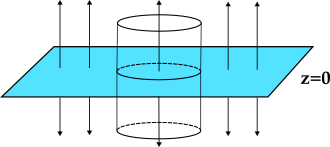
\includegraphics[width=0.5\textwidth]{images/plane}  % Adjust the width as needed
\end{wrapfigure}

Consideriamo un piano infinito, con posizione z = 0, su cui \`e presente una distribuzione di carica superficiale $\sigma$. Prendiamo una superficie Gaussiana cilindrica, con asse perpendicolare al piano come in figura. La direzione del campo elettrico \`e lungo la perpendicolare al piano $\hat{\bold{z}}$. 
\begin{equation*}
	\bold{E}(z) = E(z) \bold{\hat{z}}
\end{equation*}
Inoltre il campo elettrico per $z>0$ deve avere direzione opposta a quella del campo per $z < 0$, e dunque $E(z) = - E(-z)$.
\\

\noindent L'integrale di superficie \`e nullo lungo la superficie laterale del cilindro e gli unici contributi sono dati dalle sue basi, che ipotizziamo avere area A. Utilizzando la legge di Gauss si ha che 
\begin{equation*}
	\int_{S} \bold{E} \cdot d \bold{A} = E(z)A -E(-z)A =2E(z)A = \frac{\sigma A}{\varepsilon_0}
\end{equation*}
In modulo il campo elettrico di una distribuzione di carica per un piano infito \`e dato da 
\begin{equation}
	E(z) = \frac{\sigma}{2\varepsilon_0}
\end{equation}
Il campo elettrico \`e indipendente dalla distanza della carica sonda dal piano. Questo \`e dovuto dal fatto che il piano \`e infinito. e dunque pi\`u ci si allontana, pi\`u superficie diventa visibile.

\begin{figure}[!ht]
\centering
\begin{minipage}{0.5\textwidth}
  \centering
  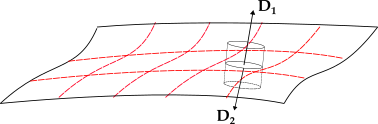
\includegraphics[width= 0.9\linewidth]{images/surface}
  \captionof{figure}{La componente normale del campo elettrico \`e discontinua.}
\end{minipage}%
\hspace{0.8cm}
\begin{minipage}{0.4\textwidth}
  \centering
  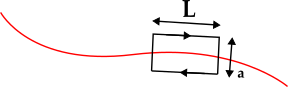
\includegraphics[width=0.8\linewidth]{images/path}
  \captionof{figure}{La componente tangenziale del campo elettrico \`e continua}
\end{minipage}
\end{figure}

Un altro importante fatto \`e che il campo elettrico non \`e continuo rispetto alle due facce del piano per una distribuzione di carica costante. Si ha che 
\begin{equation*}
	E(z \to 0^+) - E(z \to 0^-) = \frac{\sigma }{\varepsilon_0}
\end{equation*}
Tale risultato non dipende dal fatto che il piano sia finito, infatti pu\`o essere tranquillamente esteso a qualsiasi superficie con distribuzione di carica $\sigma$. Inoltre non \`e necessario che $\sigma $ sia costante  e che il campo $\bold{E}$ sia parallelo alla normale $\bold{\hat{n}}$ per ogni punto della superficie. Infatti per una superficie generica, in qualsiasi suo punto possiamo definire un cilindro Gaussiano e ripetere i calcoli per una superficie planare. Se denotiamo con $\bold{E}_{\pm}$ il campo elettrico per entrambe le parti della superficie si ha che 
\begin{equation}
	\bold{\hat{n}} \cdot \bold{E}_{+} - \bold{\hat{n}} \cdot \bold{E}_{-} = \frac{\sigma}{\varepsilon_0}
\end{equation}
e dunque il campo elettrico risulta essere discontinuo rispetto alla perpendicolare per qualsiasi superficie. In contrasto si ha che il campo tangente alla superficie \`e continuo. Per verificarlo basta considerare la circuitazione C con lato L parallela alla superficie e altezza "a" rispetto la perpendicolare.
\begin{equation*}
	\int_{C} \bold{E} \cdot d \bold{r} = LE(z')-LE(z'') = 0 
\end{equation*}
dato che $\bold{E} \cdot \bold{a} = 0$ e questo dimostra la continuit\`a delle componente parallela.

\subsection{Coppia di Piani}

\begin{wrapfigure}{r}{0.5\textwidth}  % "r" means to wrap on the right, width of the figure box
    \centering
    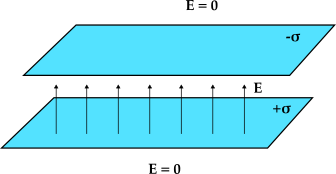
\includegraphics[width=0.5\textwidth]{images/double_plane}  % Adjust the width as needed
\end{wrapfigure}

Si consideri una coppia di piani infiniti rispettivamente a $z = 0$ e $z=a$, che possiedo una distribuzione di carica superficiale $\pm \sigma$ come in figura. Per calcolare il campo elettrico \`e sufficiente applicare il principio di sovrapposizione, considerando il campo generato dai singoli piani. Dato che un campo \`e dato dall'espressione (1.9), tenendo conto di segni e direzione si ha che 
\begin{equation}
	\bold{E} = \frac{\sigma}{\varepsilon_0} \quad 0<z<a
\end{equation}
e $\bold{E} =0$ per $z \in (-\infty,a) \cup (a,+\infty)$.

\section{Potenziale Elettrostatico. Gradiente}

\subsection{Tensione. Differenza di Potenziale Elettrostatico}
Quando su una carica $q_0$ agisce una forza $\bold{F}$ di qualsiasi natura, non necessariamente elettrostatica, ma per esempio dovuta a processi chimici o meccanici, possiamo sempre definire un campo elettrico $\bold{E}$, che prende il nome di \textit{campo elettromotore} ed \`e definito come
\begin{equation*}
	\bold{E} =  \frac{\bold{F}}{q_0} \Rightarrow \bold{F} = q_0 \bold{F}
\end{equation*}
 Notare che l'espressione ottenuta \`e uguale a quella discussa per la forza di Coulomb, ma in questo caso la si sta generalizzando a tutti i tipi di forze che possono agire su una carica. Il lavoro compiuto dalla forza $\bold{F}$ lungo un cammino $d \bold{s}$ \`e dato dal suo integrale linea 
 \begin{equation*}
 	W = \int_{C} \bold{F} \cdot d\bold{s} = q_0 \int_{C} \bold{E} \cdot d\bold{s}
 \end{equation*}
definiamo tensione elettrica tra due punti A e B lungo un percorso C il lavoro per unit\`a di carica  
\begin{equation*}
	\mathcal{E} = \frac{W}{q_0} = \int_{C}\bold{E} \cdot d\bold{s}
\end{equation*}
 In generale per un circuito chiuso C il lavoro \`e non nullo
\begin{equation*}
	W = \oint_{C} \bold{F} \cdot d\bold{s} = q_0 \oint_{C} \bold{E} \cdot d\bold{s} = q_0 \mathcal{E}
\end{equation*} 
L'integrale 
\begin{equation*}
	\mathcal{E} = \oint_{C} \bold{E} \cdot d \bold{s}
\end{equation*}
prende il nome di \textit{forza elettromotrice}. Dipende dal percorso e dalla natura del campo $\bold{E}$, ma non dalla carica $q_0$. Se il lavoro lungo un percorso chiuso C risulta essere nullo si ha la forza \`e di natura conservativa. Non dipende effettivamente dal percorso, ma solo dalla posizione di partenza e di arrivo.
\\

\noindent Nel caso di un campo $\bold{E}$ originato da una distribuzione di carica nello spazio, si ha che la forza esercitata su una carica sonda $q_0$ \`e quella di Coulomb ed \`e di natura conservativa, ovvero il suo integrale di linea su un circuito chiuso \`e nullo. Se forze di questo tipo il loro lavoro \`e dato dal teorema fondamentale del calcolo integrale in cui si considera la differenza delle primitive valutate ai due capi del percorso.
\begin{equation*}
	\int_{A}^{B} \bold{E} \cdot d \bold{s} = F(B) -F(A)
\end{equation*} 
Nel caso della forza di Coulomb tale grandezza prende il nome di \textit{differenza di potenziale elettrostatico}. Dato che la carica sonda compie lavoro contro il campo elettrico si adotta la convenzione di segno
\begin{equation}
	V_A -V_B = \int_{A}^{B} \bold{E} \cdot d\bold{s}
\end{equation}
Si osserva che il potenziale \`e definito a meno di una costante additiva. Ovvero scegliamo un punto fisso arbitrario come riferimento per la misura.
Il valoro complessivo esercitato dalla forza lungo il percorso sar\`a daro da 
\begin{equation}
	W_{AB} = q_0(V_A - V_B) = -q_0 \Delta V
\end{equation}
L'energia potenziale associata al potenziale elettrostatico \`e data 
\begin{equation*}
	W_{AB} = - \Delta U_e = U_e(A) - U_e(B)
\end{equation*}
Unendo l'espressione precedente alla (1.13) possiamo concludere che 
\begin{equation*}
	\Delta U_e =q_0\Delta V \Rightarrow U_e(A) = q_0 V_A 
\end{equation*}
Una carica $q_0$ posta in un campo elettrostatico possiede un'energia potenziale proporzionale al potenziale (definita anch'essa a meno di una costante ).
\\
\noindent In un campo elettrostatico la forza elettromotrice \`e sempre uguale a zero e quindi \`e nullo il lavoro compiuto dalla forza elettrica per ogni spostamento che riporti la carica alla posizione iniziale 
\begin{equation*}
	\mathcal{E} = \oint_{C} \bold{E} \cdot d\bold{s} = 0 \Rightarrow W = q_0 \mathcal{E} = 0
\end{equation*}
La grandezza di riferimento per misurare la differenza di potenziale \`e il $Volt = \frac{Joule}{Coulomb}$.

\subsubsection{Potenziale Elettrico di una distribuzione di carica Sferica}
Consideriamo una distribuzione di carica sferica di raggio R e densit\`a volumica $\rho$. Prendiamo come punto di riferimento per il calcolo del potenziale un punto $P_0 = + \infty $. Abbiamo che il campo elettrostatico della sfera \`e dato da 
\begin{equation*}
	\bold{E}(r) =  \left \{\begin{aligned}
		& \frac{Q}{4 \pi \varepsilon_0} \frac{1}{r^2}\hat{\mu}_{r} \quad r > R & \\[0.3cm]
		& \frac{\rho r}{3\varepsilon_0}\hat{\mu}_{r} \quad r \leq R
	\end{aligned}\right.
\end{equation*}
dunque avremo che per i punti esterni alla sfera 
\begin{equation*}
	V_{ext}(r) =\ - \int_{+ \infty}^{r} \bold{E} \cdot ds = \frac{Q}{4 \pi \varepsilon_0} \frac{1}{r} \quad r >R 
\end{equation*}
e per i punti interni si ha che
\begin{equation*}
	V_{int}(r) = V_{ext}(R) - \int_{R}^{r} dr \; \frac{\rho r}{3\varepsilon_0} = \frac{\rho R^2}{3 \varepsilon_0} - \frac{\rho}{6 \varepsilon_0}(r^2-R^2) = \frac{\rho R^2}{2 \varepsilon_0} - \frac{\rho r^2}{6 \varepsilon_0} 
\end{equation*} 
si che per $r = R$ allora $V_{int}(R) = V_{ext}(R)$.

\begin{figure}[!ht]
\centering
\begin{minipage}{0.4\textwidth}
  \centering
  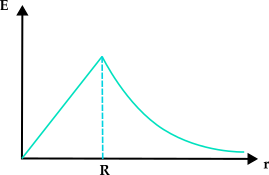
\includegraphics[width= 0.9\linewidth]{images/gsphera}
  \captionof{figure}{Intensit\`a del campo elettrico}
\end{minipage}%
\hspace{0.8cm}
\begin{minipage}{0.4\textwidth}
  \centering
  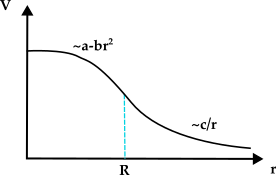
\includegraphics[width=0.9\linewidth]{images/potent}
  \captionof{figure}{Potenziale Elettrostatico}
\end{minipage}
\end{figure}
Notare che quando si fissa un punto di riferimento come $P_0 = + \infty$ tutti i cammini partono tutti da questo punto e dunque termini precedentemente calcolati per distanze pi\`u brevi compaiono in quelle pi\`u lunghe, come nel caso della misurazione del potenziale all'interno della sfera.
\subsection{Il Gradiente}

Consideriamo un generico campo scalare (funzione scalare) $\phi : \mathbb{R}^n \to \mathbb{R} $. Date le coordinate cartesiane $x_i $ per i =1,...,n, il gradiente di $\phi$ \`e dato da 
\begin{equation*}
	\nabla \phi = \left [ \frac{\partial \phi}{\partial x_1},...,\frac{\partial \phi}{\partial x_n} \right ] 
\end{equation*}
Differenziare un campo scalare ci porta ad avere un campo vettoriale. La possibilit\`a di poter definire il gradiente di una funzione scalare ci permette di definire il differenziale di $\phi$, ovvero
\begin{equation*}
	d\phi = \sum_{i} \frac{\partial \phi}{\partial x_i}dx_i = \nabla \phi \cdot d\bold{s}
\end{equation*}
che definisce la variazione di $\phi$ rispetto ad uno spostamento $d\bold{s} = [dx_1,...,dx_n]^T$. Tramite il gradiente di $\phi$ possiamo identificare la direzione e verso di massima crescita
\begin{equation*}
	df = ||\nabla \phi||\;||d\bold{s}|| \cos \theta 
\end{equation*}
e dunque $df$ \`e massimo quando $\nabla \phi$ \`e parallelo allo spostamento $d\bold{s}$.
\\
\noindent Nella sezione precedente abbiamo definito il potenziale elettrostatico che \`e una funzione scalare, se consideriamo una sua variazione infinitesima avremo che
\begin{equation*}
	dV = - \bold{E} \cdot d\bold{s} \iff dV = \nabla V \cdot d\bold{s} 
\end{equation*}
e quindi si ha che $\bold{E} = - \nabla V$, ovvero il campo elettrico \`e proporzionale e contrario al potenziale. Se moltiplichiamo tuto per una carica $q_0$ si ha che 
\begin{equation*}
	\bold{F}_e = - \nabla U_e
\end{equation*}
che \`e il risultato che ci aspettiamo di ottenere per una forza di natura conservativa.
\\
\noindent Si noti che fino a questo punto si \`e data una definizione del gradiente dipendente dalle coordinate cartesiane, ma esso pu\`o essere espresso rispetto ad altri sistemi di coordinate.
\\

\noindent Una conseguenza importante per le forze conservative \`e che dato un potenziale V(x,y,z), essendo una funzione scalare \`e possibile definirne le curve di livello, ed essendo $\bold{E} = - \nabla V$ si avr\`a che il campo elettrico in tutti i punti dello spazio in cui \`e definito \`e ortogonale a tali curve.
\subsubsection{Esempio - Carica Puntiforme}

\begin{wrapfigure}{r}{0.5\textwidth}
  \begin{center}
    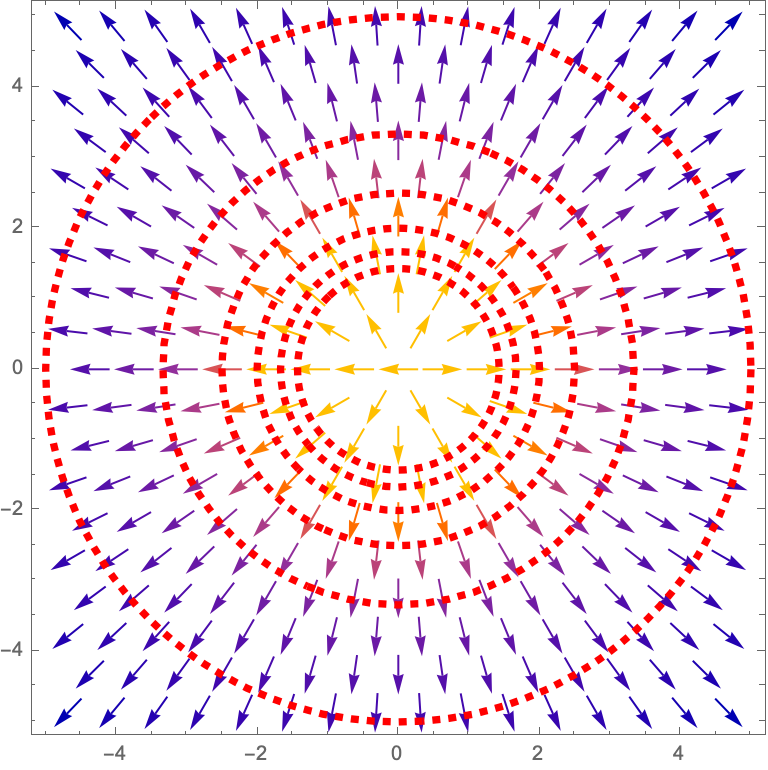
\includegraphics[width=0.4\textwidth]{images/contour}
  \end{center}
\end{wrapfigure}
Rispetto ad un sistema di coordinate cartesiane e prendendo $P_0 = + \infty$ come riferimento di misura si ha che il potenziale per una carica puntiforme posta nell'origine del sistema \`e dato da


\begin{equation*}
	V(x,y) = \frac{Q}{4 \pi \varepsilon_0} \frac{1}{\sqrt{x^2+y^2}}
\end{equation*}
 

\vspace{0.4cm}
\noindent calcolando le sue curve di livello avremo in figura che il campo elettrico $\bold{E}$ \`e ortogonale ad esse come in figura (circonferenza tratteggiate in rosso).
\newpage

\begin{lstlisting}{language = Mathematica}
Mathematica Snippets

V[x_, y_, q_] := (1/Sqrt[x^2 + y^2])
E1x[q_, x_, y_, x0_, y0_] := ((x - x0)/((x - x0)^2 + (y - y0)^2)^(1.5))
E1y[q_, x_, y_, x0_, y0_] := ((y - y0)/((x - x0)^2 + (y - y0)^2)^(1.5))

Show[VectorPlot[{E1x[Q, x, y, 0, 0], E1y[Q, x, y, 0, 0]}, {x, -5, 
   5}, {y, -5, 5}],
 ContourPlot[V[x, y, Q] , {x, -5, 5}, {y, -5, 5}, 
  ContourStyle -> Directive[Red, Dashed, Thickness[0.01]], 
  ContourShading -> None]]
\end{lstlisting}

\subsubsection{Esempio - Oscillatore Armonico}

\begin{wrapfigure}{r}{0.5\textwidth}
  \begin{center}
    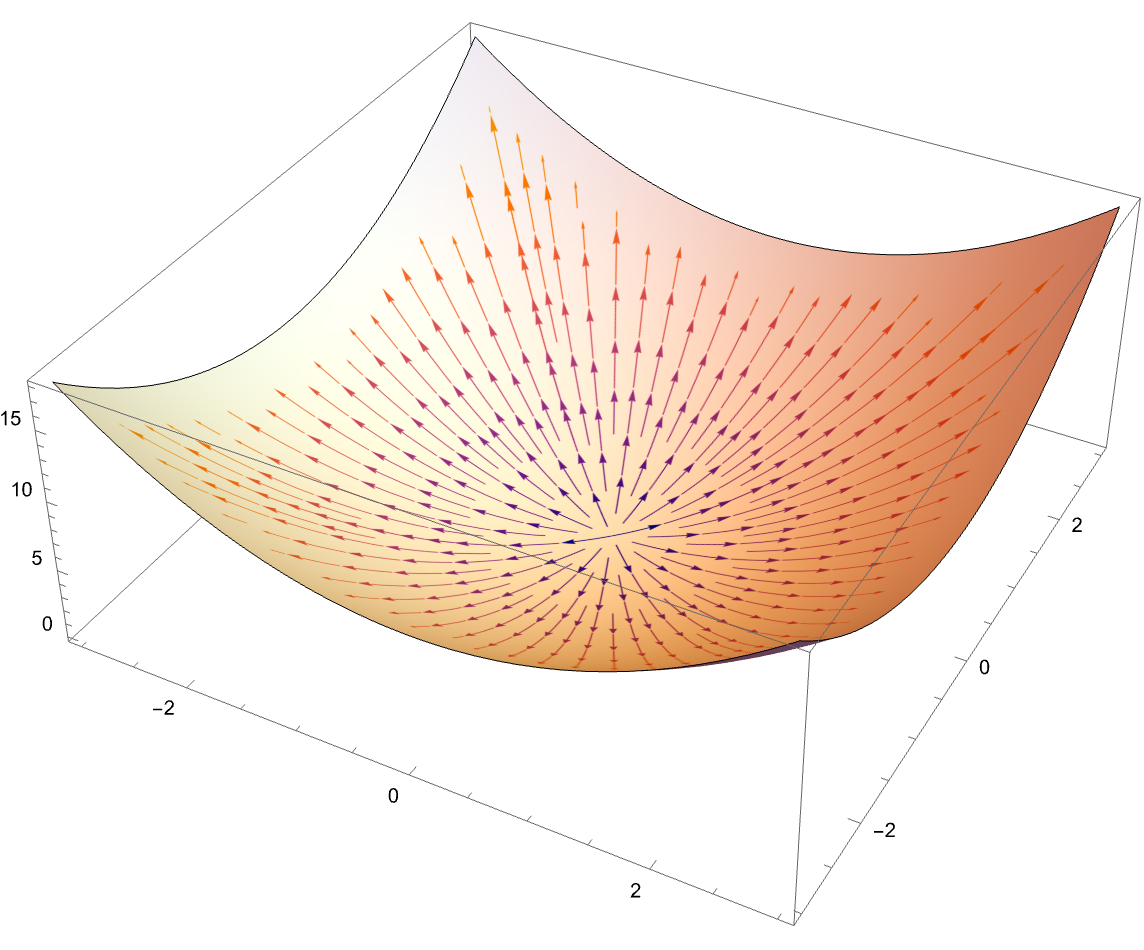
\includegraphics[width=0.5\textwidth]{images/harmonic}
  \end{center}
\end{wrapfigure}
Consideriamo una particella sottoposta ad una forza elastica vincolata a muoversi in una sola direzione. Ipotizziamo che non sia presenti attriti, dunque l'energia del sistema sar\`a data dalla funzione 
\begin{equation*}
	E(x,y) = \frac{1}{2}my^2 + \frac{1}{2}kx^2
\end{equation*}
rispettivamente il gradiente sar\`a un vettore della forma
\begin{equation*}
	\nabla E = \left [ \begin{array}{c}
		kx \\
		my
	\end{array} \right ]
\end{equation*}
e sar\`a tangente alla superficie data da E(x,y), come in figura.

\begin{lstlisting}
Mathematica Snippets 
	
Plot3D[(x^2 + y^2), {x, -3, 3}, {y, -3, 3}, 
 PlotStyle -> 
  Texture[StreamPlot[
    Evaluate[D[(x^2 + y^2), {{x, y}}]], {x, -3, 3}, {y, -3, 3}, 
    Frame -> None, ImageSize -> Large]], Mesh -> None, 
 ImageSize -> Large, PlotPoints -> 35]
\end{lstlisting}
\subsection{Potenziale per una distribuzione di cariche }

I risultati ottenuti nel paragrafo sul potenziale elettrostatico sono facilmente estendibili al caso in cui un campo elettrostatico \`e dato dalla distribuzione di pi\`u cariche puntiformi $q_1,...,q_n$, per farlo \`e sufficiente utilizzare il principio di sovrapposizione.
\\
Se consideriamo una carica sonda $q_0$ il lavoro compiuto per spostare la carica all'interno dell campo elettrostatico generato dalla distribuzione di cariche \`e dato da 
\begin{equation*}
	W =\int_{A}^{B} \bold{F} \cdot d\bold{s} = q_0 \int_{A}^{B} \bold{E} \cdot d\bold{s}
\end{equation*}
dato che il campo complessivo \`e dato da $\bold{E} = \sum_{i} \bold{E}_i$ dove $\bold{E}_i$ \`e il campo generato dalle singole cariche, dunque il potenziale assume la forma
\begin{equation*}
	\int_{A}^{B}\bold{E} \cdot d \bold{s} = \sum_{i}\int_{A}^{B} \bold{E}_i \cdot d\bold{s} = \sum_{i} \int _{A}^{B} \frac{q_i}{4 \pi \varepsilon_0 r_i^2} \; \hat{\mu}_i \cdot d\bold{s}
\end{equation*}
e quindi la differenza di potenziale \`e data d a
\begin{equation*}
	V(A) - V(B) = \sum_{i}\frac{q_i}{4 \pi \varepsilon_0 r_{A,i}^2} - \sum_{i}\frac{q_i}{4 \pi \varepsilon_0 r_{B,i}^2} 
\end{equation*}
Posto V(B) = 0 per $B = \infty$ si ha che 
\begin{equation}
	V(r) = \int_{P}^{\infty} \bold{E}  \cdot d \bold{s} = \sum_{i}\frac{q_i}{4 \pi \varepsilon_0 r_{i}^2}
\end{equation}
Tale risultato indica che il potenziale elettrostatico generato da un sistema di cariche puntiformi \`e uguale alla somma dei potenziali generati singolarmente dalle cariche. Possiamo estende il risultato per distribuzioni di carica continue 
\begin{equation}
	\begin{aligned}
		& V(r) = \frac{1}{4 \pi \varepsilon_0}\int_{C} ds \; \frac{\lambda(r)}{|r-r'|} & \\[0.5cm]
		& V(r) = \frac{1}{4 \pi \varepsilon_0} \int_{S} d\Sigma \; \frac{\sigma (r)}{|r-r'|} & \\[0.5cm]
		& V(r) = \frac{1}{4 \pi \varepsilon_0} \int_{V}dV \;  \frac{\rho(r)}{|r-r'|} 
	\end{aligned}
\end{equation}
Il potenziale elettrostatico risulta essere una funzione del punto, continua e derivabile, che pu\`o essere calcolabile una volta conosciuta la distribuzione delle cariche sorgente, indipendentemente dalla presenza di $q_0$. Infatti ci si rivolge ad esso anche come campo scalare. A differenza del campo vettoriale ci\`o che \`e significativo non \`e il valore che un potenziale assume in un punto, ma la sua variazione rispetto ad un riferimento fissato.

\subsection{Energia Potenziale Elettrostatica}

 L'energia potenziale $U(\bold{r})$ di una particella $q_0$ immersa nel campo elettrostatico $\bold{E}$, \`e data dal lavoro compiuto per spostarla da infinito ad un certo punto P dello spazio

\begin{equation*}
	U(\bold{r}) = -	q_0\int_{\infty}^{P} \bold{E} \cdot d\bold{r} = q_0 \int_{\infty}^{P} \nabla \phi \cdot d\bold{r} = q_0 \; \phi(\bold{r})  
\end{equation*}
dove assumiamo che $\phi(\bold{r}) \to 0$ per $\bold{r} \to \infty$.
\\

Consideriamo una distribuzione di carica formata dal cariche $q_i$ con posizioni $r_i$ nello spazio . Il potenziale elettrostatico immagazzinato in questa configurazione coincide con il lavoro necessario ad assemblare la configurazione della distribuzione di carica discreta (questo \`e dovuto al fatto che se dovessimo rilasciare le cariche la loro energia cinetica sarebbe coincidente con il potenziale latente del sistema). Dunque quanto lavoro \`e necessario per assemblare la configurazione della distribuzione di carica ?
\\

Fissiamo la prima carica nello spazio in $\bold{r_1}$. Il lavoro $W_1 =0$ dato che non \`e presente campo elettrostatico, poich\`e una carica non esercita forza su se stessa. Per spostare una seconda carica \`e necessario un lavoro di 
\begin{equation*}
	W_2 = \frac{q_1q_2}{4 \pi \varepsilon_0} \frac{1}{|\bold{r_1} - \bold{r_2}|}
\end{equation*}
Notare che se le due cariche hanno lo stesso segno $q_1q_2 > 0$ e dunque $W_2 > 0$, e dunque bisogna immettere lavoro nel sistema affinch\`e queste si avvicinino. Se $q_1q_2 < 0$ allora $W_2 < 0$ e quindi le particelle si avvicinano per mutua attrazione.
\\
Se ora avviciniamo una terza carica questa si dovr\`a spostare all'interno del campo elettrico generato dalle cariche $q_1$ e $q_2$ e dunque il lavoro necessario \`e 
\begin{equation*}
	W_3 = \frac{q_3}{4 \pi \varepsilon_0} \left [  \frac{q_2}{|\bold{r_2} - \bold{r_3}|} + \frac{q_1}{|\bold{r_1}-\bold{r_3}}\right ] 
\end{equation*}
e cos\`i via aggiungendo altre particelle. Il lavoro complessivo per assemblare la distribuzione di carica \`e data dall'energia potenziale immagazzinata nel sistema.
\begin{equation}
	U = \sum_{i=1}^NW_i = \frac{1}{2}\frac{1}{4 \pi \varepsilon_0}\sum_{i}\sum_{i\neq j} \frac{q_iq_j}{|\bold{r_i}-\bold{r_j}|}
\end{equation}
Se vogliamo misurare il potenziale nel punto $\bold{r_i}$ dovuto alle cariche $q_j,\;j\neq i$ si ha che
\begin{equation*}
	\phi(\bold{r_i}) = \frac{1}{4 \pi \varepsilon_0} \sum_{j \neq i} \frac{q_j}{|\bold{r_i}-\bold{r_j}|}
\end{equation*} 
e dunque possiamo riscrivere l'energia potenziale come 
\begin{equation}
	U = \frac{1}{2}\sum_{i=1}^Nq_i \phi(\bold{r_i})
\end{equation}
che rappresenta l'energia potenziale per una distribuzione discreta di cariche. Possiamo generalizzare tale risultato alle distribuzioni continue $\rho(\bold{r})$ definite una regione chiusa dello spazio. L'energia associata a una distribuzione continua \`e data da 
\begin{equation}
	U = \frac{1}{2} \int_V dV \; \rho(\bold{r})\phi(\bold{r})
\end{equation}
Ritorneremo successivamente su questa equazione quando introdurremo l'operatore di divergenza per un campo vettoriale.

\subsection{Esempi ed Esercizi}

\subsubsection{Potenziale di una distribuzione di carica superficiale a simmetria sferica}

Data una densit\`a di carica areica $\sigma$ costante distribuita su una sfera di raggio R, vogliamo determinare il potenziale $\phi(r)$ ad una generica distanza r da essa.

\newpage

\begin{figure}[!ht]
\vspace{0.1in}
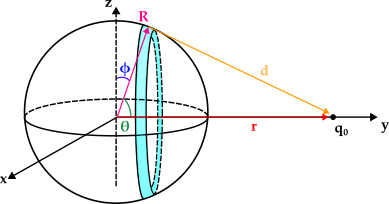
\includegraphics[width =10cm]{images/ringsym}	
\centering
\vspace{0.2in}
\end{figure}
Utilizzando il teorema di Carnot abbiamo che la distanza d data dalla diagonale in figura pu\`o essere espressa come 
\begin{equation*}
	d = \left [ R^2+r^2 -2rRcos\theta \right ]^{1/2} = ||\bold{R} -\bold{r}||
\end{equation*}
applicando l'espressione del potenziale per una distribuzione di carica continua si ha che 

\begin{equation*}
\begin{aligned}
	 & \phi(r) = \frac{1}{4 \pi \varepsilon_0} \int_{A} d\Sigma \; \frac{\sigma }{d} = \frac{1}{4 \pi \varepsilon_0} \int_{0}^{2\pi}d \varphi \int_{0}^{\pi}d\theta \; \frac{\sigma R^2 \sin\theta }{d} =  \frac{2\pi \sigma R^2}{4\pi \varepsilon_0} \int_{0}^{\pi}d\theta \; \frac{\sin \theta}{d} =  \\[0.5cm]
	& = \frac{Q}{8 \pi \varepsilon_0} \frac{1}{Rr} \left [(R^2+r^2 - 2rR \cos \theta)^{1/2} \right ]_{0}^{\pi} = \\[0.5cm]
	&  = \frac{Q}{8 \pi \varepsilon_0} \frac{1}{Rr} \left [(R^2+r^2+2rR)^{1/2} - (R^2+r^2-2rR)^{1/2} \right ] = \\[0.5cm]
	& = \frac{Q}{8 \pi \varepsilon_0} \frac{1}{Rr} \left [(R+r)-|R-r| \right ] 
\end{aligned}
\end{equation*}
\begin{wrapfigure}{r}{0.4\textwidth}
\vspace{-1.7cm}
  \begin{center}
    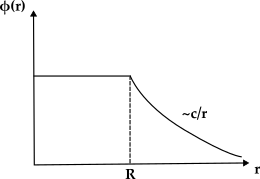
\includegraphics[width=0.4\textwidth]{images/chargesurf}
  \end{center}
\end{wrapfigure}
Per $Q = 4\pi R^2 \sigma $ (Carica di un anello) il potenziale \`e dato da
\begin{equation*}
	\phi(r) = 
	\left \{ \begin{array}{l}
		 \frac{Q}{4 \pi \varepsilon_0} \frac{1}{r} \quad r >R \\
		 \frac{Q}{4 \pi \varepsilon_0} \frac{1}{R} \quad r < R
		 \end{array}\right.
\end{equation*}
Il potenziale interno \`e costante e pari al potenziale della superficie.

\subsubsection{Potenziale per una distribuzione di carica lineica infinita}

\begin{wrapfigure}{r}{0.4\textwidth}
  \begin{center}
    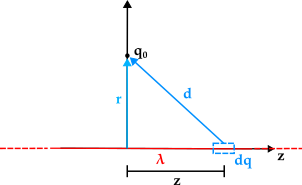
\includegraphics[width=0.4\textwidth]{images/lineinf}
  \end{center}
\end{wrapfigure}

Calcoliamo il potenziale elettrostatico per un filo di estensione infinita e carica $\lambda $ parallelo alla direzione $\hat{\bold{z}}$. Utilizzando la definizione di potenziale per una distribuzione di carica infinita 
\begin{equation*}
	\phi(r) = \frac{1}{4 \pi \varepsilon_0} \int_{-\infty}^{+\infty} dz \; \frac{\lambda}{d} = \frac{\lambda }{4 \pi \varepsilon_0} \int_{-\infty}^{+\infty} \frac{dz}{[z^2+r^2]^{1/2}}
\end{equation*}
nel calcolo si ha un problema in quanto 
\begin{equation*}
	\phi(r) \simeq \int \frac{1}{r}
\end{equation*}
e dunque il potenziale \`e divergente ad infinito. Per evitare questo problema calcoliamo l'integrale su un intervallo chiuso $[-L,L]$, con $L >> r$.
\begin{equation*}
	\phi(r) = \frac{1}{4 \pi \varepsilon_0} \int_{-L}^{L}dz \; \frac{\lambda}{[r^2+z^2]^{1/2}} = \frac{\lambda}{4 \pi \varepsilon_0} \ln \left[ \frac{(1+  r^2/L^2)^{1/2}+1}{(1+r^2/L^2)^{1/2} -1}\right ]
\end{equation*}
dato che $L >> r$ possiamo sviluppare con Taylor rispetto a $\frac{r^2}{L^2}$
\begin{equation*}
	\begin{aligned}
		& \phi(r) = \frac{\lambda}{4 \pi \varepsilon_0} \ln \left [ \frac{4L^2+r^2}{r^2} \right ] \simeq \frac{\lambda}{4 \pi \varepsilon_0} \ln \left[\frac{2L}{r} \right ]^2 = \frac{\lambda}{2 \pi \varepsilon_0} \ln \left[\frac{2L}{r}\right ] = \\[0.5cm]
		& = \frac{\lambda}{2 \pi \varepsilon_0} \left [ \ln \left ( \frac{1}{r} \right ) + \ln(2L)\right] = \frac{\lambda}{2 \pi \varepsilon_0} \ln \left ( \frac{1}{r} \right) + \text{cost} 
	\end{aligned}
\end{equation*}
in questo modo riusciamo a mettere a zero il potenziale per $r \to \infty$.
Utilizzando la relazione tra campo elettrostatico e gradiente del potenziale abbiamo che 
\begin{equation*}
	\bold{E} = - \frac{\partial \phi}{\partial r} \; \hat{\mu}_{r} = \frac{\lambda}{2 \pi \varepsilon_0} \frac{1}{r} \;\hat{\mu}_{r}
\end{equation*}
ottenendo il campo per una distribuzione di carica lineare e con estensione infinita.
\newpage

\subsubsection{Potenziale per una distribuzione di carica sulla superficie di un disco}

\begin{wrapfigure}{r}{0.4\textwidth}
\vspace{-0.3cm}
  \begin{center}
    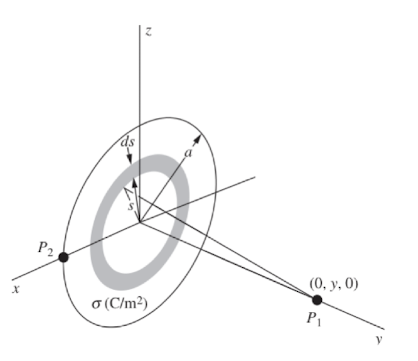
\includegraphics[width=0.4\textwidth]{images/disco}
  \end{center}
\end{wrapfigure}

Data una distribuzione di carica superficiale $\sigma$ per un disco di raggio R, vogliamo determinare il potenziale elettrostatico in funzione della posizione. Avremo che presa una distribuzione di carica infinitesima circolare con $dQ = 2 \sigma \pi rdr$, l'espressione per una distribuzione di carica continua del potenziale \`e data da
\begin{equation*}
\begin{aligned}
	& \phi(0,y,0) = \frac{1}{4 \pi \varepsilon_0}\int_{0}^{R} \frac{2 \pi \sigma rdr}{[r^2 + y^2]^{1/2}}\\[0.5cm] & = \frac{\sigma}{2 \varepsilon} \int_{0}^{R}dr \; \frac{r}{[r^2+y^2]^{1/2}} = \frac{\sigma}{2 \varepsilon} \left [\sqrt{r^2+y^2}\right ]_{0}^{R} = & \\[0.5cm]
	& = \frac{\sigma}{2 \varepsilon_0}\left[ \sqrt{R^2+y^2} - |y| \right ]
\end{aligned}
\end{equation*}
Dato che \`e presente un modulo all'interno dell'espressione del potenziale si ha che, questo assume valori diversi lungo y per $y>0$ o $y<0$.

\begin{equation*}
	\phi(y) = \left \{ \begin{array}{l}
		\frac{\sigma }{2 \varepsilon_0} \left [ \sqrt{R^2+y^2} - y \right ] \quad y > 0 \\[0.5cm]
		\frac{\sigma}{2 \varepsilon_0} \left [ \sqrt{R^2+y^2} + y \right ] \quad y < 0
	\end{array}\right.
\end{equation*}
\\

\noindent Il potenziale \`e continuo in $y = 0$ a differenza del campo elettrostatico che presenta un punto di discontinuit\`a a cuspide.
\begin{equation*}
	\bold{E} = - \nabla \phi = -\frac{d \phi}{dy}\Big |_{y=0} = \left \{ \begin{array}{l}
		\frac{\sigma}{2 \varepsilon_0} \quad y>0 \\
		-\frac{\sigma}{2 \varepsilon_0} \quad y < 0
	\end{array}\right.
\end{equation*}
\begin{remark}	
\end{remark}

\begin{itemize}
	\item Per $y \to 0^{\pm}  $ si ha che il potenziale del disco coincide con quello di un piano infinito.
	\item Nel limite in cui $y >> R$, il comportamento del potenziale \`e uguale a quello di una carica puntiforme.
	\begin{equation*}
		\phi(y) = \frac{\sigma}{2 \varepsilon_0}y \left [ \left ( 1+ \frac{R^2}{y^2}\right)^{1/2} - 1\right ] \simeq_{\text{Taylor}} \frac{\sigma R^2}{4  \varepsilon_0} \frac{1}{y}
	\end{equation*}
\end{itemize}
e dunque il campo scalare ha una discontinuit\`a in $y =0 $.
 
\begin{figure}[!ht]
\vspace{0.1in}
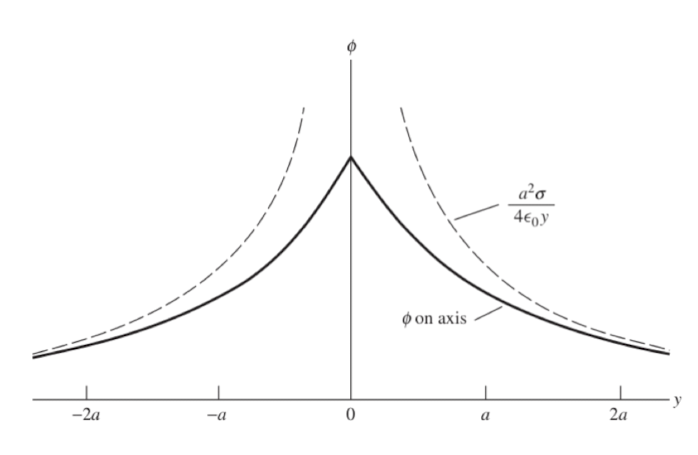
\includegraphics[width = 10cm]{images/disco_discont.png}	
\centering
\vspace{0.1in}
\end{figure}

\section{Divergenza di un  Campo Vettoriale}

La divergenza di un campo vettoriale ci permette di esprimere la legge di Gauss in forma differenziale, legando le propriet\`a locali del campo elettrostatico alla distribuzione di carica. In sostanza consideriamo la variazione infinitesima del campo elettrostatico in un intorno di un punto dello spazio.
\\

\noindent Presa una regione di spazio V chiusa e al cui interno \`e contenuta della carica, abbiamo visto che questa fluisce attraverso la superficie data dal bordo $S = \partial V$ di S. Il flusso \`e dato dall'equazione
\begin{equation*}
	\phi(\bold{F}) = \int_{S} \bold{F} \cdot d\bold{A}
\end{equation*} 
Se immaginiamo di affettare la regione di spazio, otteniamo diverse sezioni $V_i$ attraverso cui parte del flusso passa attraverso, di conseguenza possiamo riscrivere il flusso totale come
\begin{equation*}
	\phi(\bold{F}) = \sum_{i=1}^N \int_{ S_i} \bold{F} \cdot d\bold{A}_i
\end{equation*}
ovvero la somma dei contributi delle singole regioni attraverso cui il campo passa attraverso. Per $N \to \infty$, ovvero aumentando i sezionamenti si ha che i rispettivi volumi $V \to 0$ e dunque ogni singolo contributo descrive un flusso locale.
\\

\noindent Il problema con questa definizione \`e che $\int_{S_i} \bold{F} \cdot d\bold{A}_i$ dipende dalla scelta del volume $V_i$ e dunque dalla scelta della superficie $S_i$ e dunque non si ha una buona misura del campo locale.
\\
Per esempio se prendiamo un volume $V_i$ se lo raddoppiamo o lo dimezziamo il risultato della misura del flusso aumenta e diminuisce (per $\bold{F}$ costante) e questo non ci permette di avere una buona stima di come sia cambiato il campo nelle regioni. Se $\bold{F}$ non \`e costante il problema \`e che riducendo il volume a 0 anche il flusso diventa nullo.
\\

Per dare una buona definizione locale di flusso consideriamo il suo valore medio rispetto al volume $V_i$
\begin{equation*}
	\langle \phi(\bold{F}) \rangle = \frac{1}{V}\int_{S_i} \bold{F} \cdot d \bold{A}_i
\end{equation*}
Tale equazione ci permette di definire la divergenza del campo $\bold{F}$ nel seguente modo
\begin{equation}
	\text{div}\bold{F} = \lim_{V_i \to 0} \frac{1}{V_i} \int_{S_i} \bold{F} \cdot d\bold{A}_i
\end{equation}
La divergenza di un vettore \`e una grandezza scalare che misura il flusso (locale) uscente da una superficie normalizzata al volume da essa racchiuso. Tale definizione ci rende la misura della divergenza del campo indipendente dalla geometria dei volumi.
\\

\noindent Uno dei risultati pi\`u importanti della teoria dei campi vettoriali \`e \textit{il teorema di divergenza di Gauss}, la cui espressione possiamo ottenere, considerando
\begin{equation}
	\int_{S}\bold{F} \cdot d\bold{A} = \lim\limits_{\substack{N \to +\infty \\[0.1cm] V_i \to 0}}\left [ \sum_{i=1}^N \frac{1}{V_i} \int_{S_i} \bold{F} \cdot d\bold{A}_i \right ] = \int_{V}\text{div}\bold{F} \; dV
\end{equation}

\begin{remark}
\end{remark}
\begin{itemize}
	\item Il teorema di Gauss \`e una propriet\`a matematica che vale per qualsiasi campo vettoriale.
	\item Il vettore $\bold{E}$ soddisfa una legge fisica (la legge di Gauss) che collega il flusso alla distribuzione di carica.
\end{itemize}	

\noindent Se consideriamo il campo elettrostatico $\bold{E}$ generato da una distribuzione di carica continua $\rho$ per la legge di Gauss abbiamo che
\begin{equation*}
	\phi(\bold{E})=\int_{S}\bold{E} \cdot d\bold{A} = \frac{1}{\varepsilon_0} \int_{V} \rho \; dV
\end{equation*}
per il flusso del campo possiamo applicare il teorema di divergenza di Gauss, in questo modo abbiamo che 
\begin{equation*}
	\int_{V} \text{div}\bold{E} \; dV = \frac{1}{\varepsilon_0} \int_{V} \rho \; dV
\end{equation*}
Dato che tale uguaglianza \`e soddisfatta per ogni volume e superficie, l'uguaglianza deve essere soddisfatta anche dai termini integrandi, definendo in questo modo \textit{la forma differenziale della legge di Gauss}.
\begin{equation}
	\text{div}\bold{E} = \frac{\rho}{\varepsilon_0} 
\end{equation}
Il ragionamento logico con cui si \`e ottenuta la divergenza di un campo fa s\`i che la definizione (1.20) non dipenda da un sistema di coordinate e quindi vale per tutti. Da un punto di vista applicativo per\`o risulta essere poco utile e quindi abbiamo bisogno di darne una seconda definizione pi\`u funzionale.

\subsection{Espressione della Divergenza in coordinate cartesiane}

Prendiamo un punto $\bold{x_0}$ dello spazio e consideriamolo come centro di un volume infinitesimo $dV=dxdydz$, data la presenza di un campo vettoriale $\bold{F}$ vogliamo determinare la divergenza localmente in coordinate cartesiane. Partendo dalla definizione di divergenza ed esplicitando il prodotto scalare dell'integrando si avr\`a che 
\begin{equation*}
 \text{div}\bold{F} =  \lim_{V \to 0} \frac{1}{V} \int_{S} \bold{F} \cdot d\bold{A} = \lim_{V \to 0 } \frac{1}{V} \left [ \int_{S} F_{x}\text{dydz} + \int_{S} F_y \text{dxdz} + \int_{S} F_z \text{dxdy}\right ]
	 \end{equation*}
utilizzando il teorema della media integrale per una delle facciate del cubo si ha per esempio che 
\begin{equation*}
	\int_{S_1}\bold{F}\cdot \bold{\hat{n}}(\text{dydz}) \simeq F_x(x_0+\frac{dx}{2},y,z)\Delta y \Delta z
\end{equation*}
in cui consideriamo la componente 'x' del campo valutata in un generico punto. 
 
\begin{figure}[ht]
\vspace{0.1in}
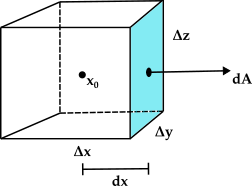
\includegraphics[width = 5cm]{images/cube}	
\centering
\vspace{0.1in}
\end{figure}
Possiamo reiterare lo stesso ragionamento per la faccia opposta, cambiando segno
\begin{equation*}
	-\int_{S_2}\bold{F}\cdot \bold{\hat{n}}(\text{dydz}) \simeq -F_x(x_0-\frac{dx}{2},y,z)\Delta y \Delta z
\end{equation*}
se vogliamo ottenere il contributo complessivo dato dall'addendo $\int_{S} F_{x}\text{dydz}$ dobbiamo considerare la superficie $S = S_1+S_2$ e quindi si ha che 
\begin{equation*}
	\int_{S} F_{x}\text{dydz} \simeq F_x(x_0+\frac{dx}{2},y,z)\Delta y \Delta z -F_x(x_0-\frac{dx}{2},y,z)\Delta y \Delta z
\end{equation*}
normalizzando rispetto al volume otteniamo l'equazione 
\begin{equation*}
	\frac{1}{V}\int_{S} F_{x}\text{dydz} \simeq \frac{F_x(x_0+\frac{dx}{2},y,z)-F_x(x_0-\frac{dx}{2},y,z)}{\Delta x}
\end{equation*}
e prendendo il limite per $V \to 0$ possiamo conclude che 
\begin{equation*}
	\lim_{V \to 0} \frac{1}{V}\int_{S} F_{x}\text{dydz} \simeq \lim_{\Delta x  \to 0} \frac{1}{V}\int_{S} F_{x}\text{dydz} \simeq \frac{F_x(x_0+\frac{dx}{2},y,z)-F_x(x_0-\frac{dx}{2},y,z)}{\Delta x} = \frac{\partial F_{x}}{\partial x }
\end{equation*}

Ripetendo i medesimi ragionamenti per gli addendi possiamo concludere che 
\begin{equation}
	\text{div}\bold{F} = \frac{\partial F_x}{\partial x} + \frac{\partial F_y}{\partial y} + \frac{\partial F_z}{\partial z}
\end{equation}
esprimendo la divergenza rispetto ad un sistema di coordinate cartesiane.
\\

\noindent Possiamo esprimere la divergenza utilizzando l'operatore gradiente 
\begin{equation*}
	\nabla = \frac{\partial }{\partial x_i}\bold{e}_i
\end{equation*}
che rappresenta sia un operatore che un vettore. Lo definiamo operatore perch\`e agisce sugli sugli spazi di funzione. Se facciamo agire l'operatore sul campo vettore $\bold{F}$ definito da una mappa
\begin{equation*}
	\bold{F} : \mathbb{R}^N \to \mathbb{R}^N
\end{equation*}
definiamo l'azione di $\nabla $ su $\bold{F}$ come il loro prodotto vettoriale 
\begin{equation}
	\text{div} \bold{F} = \nabla \cdot \bold{F} 
\end{equation}
in questo manteniamo la propriet\`a in cui la divergenza di un campo vettoriale deve restituire un campo scalare.
\\

\noindent Da un punto di vista fisico il segno della divergenza ci dice che se $\nabla \cdot \bold{F}>0$ localmente si ha un flusso netto uscente dal volume infinitesimo, viceversa per $\nabla \cdot \bold{F} < 0$ il flusso netto \`e localmente entrante nel volume.
\\

\noindent La forma della divergenza espressa rispetto all'operatore gradiente, ci permette di riscrivere la forma differenziale della legge di Gauss come
\begin{equation}
\boxed{
	\nabla \cdot \bold{E} = \frac{\rho}{\varepsilon_0}}
\end{equation}
questa espressione definisce una delle equazioni fondamentali dell'elettromagnetismo e prende il nome di \textit{prima equazione di Maxwell per l'elettrostatica}.


\subsection{Propriet\`a dell' operatore gradiente }

L'operatore gradiente \`e un operatore differenziale lineare, ovvero valgono le seguenti propriet\`a 
\begin{equation}
\begin{aligned}
\nabla(\alpha \phi+\psi) & =\alpha \nabla \phi+\nabla \psi \\
\nabla \cdot(\alpha \mathbf{F}+\mathbf{G}) & =\alpha \nabla \cdot \mathbf{F}+\nabla \cdot \mathbf{G}
\end{aligned}
\end{equation}
per ogni campo scalare $\phi$ e $\psi$, campo vettoriale $\bold{F}$ e $\bold{G}$ e costante $\alpha$.

Inoltre vale la propriet\`a di Leibniz, che \`e una generalizzazione della regola del prodotto, ovvero
\begin{equation}
\begin{aligned}
\nabla(\phi \psi) & =\phi \nabla \psi+\psi \nabla \phi \\
\nabla \cdot(\phi \mathbf{F}) & =(\nabla \phi) \cdot \mathbf{F}+\phi(\nabla \cdot \mathbf{F})
\end{aligned}
\end{equation} 
per $\phi,\psi$ campi scalari e $\bold{F}$ campo vettoriale.

\subsection{Esempi ed Esercizi}

\subsubsection{Campo elettrostatico di una lastra infinita}

\begin{wrapfigure}{r}{0.5\textwidth}
  \centering
  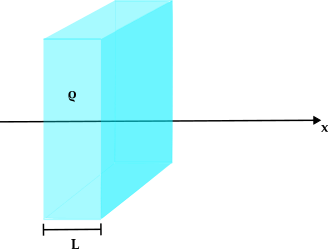
\includegraphics[width=0.5\textwidth]{images/lastra}
\end{wrapfigure}

Calcoliamo il campo elettrostatico per una lastra di superficie infita e spesso L, data una densit\`a di carica di volume $\rho$ uniforme. 
\\

\noindent Come fatto per gli esercizi precedenti per ragioni di simmetria sappiamo che il campo $E_z = E_y = 0$.
\\ Questa volta per\`o utilizziamo la forma differenziale dell'equazione di Gauss per calcolare il campo.

\begin{equation*}
	\nabla \cdot \bold{E} = \frac{\rho}{\varepsilon_0} \iff \frac{\partial E_x(x)}{\partial x} = \frac{\rho}{\varepsilon_0}
\end{equation*}
risolvendo l'equazione differenziale per quadrature si ha che 
\begin{equation*}
	E_x(x) = \frac{\rho}{\varepsilon_0}x + A
\end{equation*}
dove il termine A \`e la costante d'integrazione per un integrale indefinito.
\begin{remark}
Si noti che se consideriamo $\bold{E}(x) = \left ( \frac{\rho}{\varepsilon_0}x+A \right ) \hat{\mu}_{x}$	 e se applichiamo l'operatore gradiente al campo si ha che 
\begin{equation*}
	\nabla \cdot \bold{E} = \nabla \cdot \left ( \frac{\rho}{\varepsilon_0}x \hat{\mu}_{x}\right) + \nabla \cdot (A \hat{\mu}_x) = \frac{\rho}{\varepsilon_0} 
\end{equation*}
dunque il termine $\nabla \cdot (A \hat{\mu}_x) = 0$. In genere un campo vettoriale $\bold{F}$ \`e caratterizzato dalla divergenza a meno di un vettore a divergenza nulla. Che possiamo parafrasare pensato al fatto che esista una parte del campo che non contribuisce al flusso netto attraverso una superficie.
\end{remark}
Ritornando alla risoluzione del problema, abbiamo bisogno di definire delle condizioni al contorno che ci determinino il valore della costante A, per farlo osserviamo che se poniamo una carica esploratrice $q_0$ in $\bold{x} = 0$ (che coincide con il centro della lastra) avremo che la forza esercitata sulla carica \`e nulla per simmetria e dunque anche $\bold{E} = 0$. Risolvendo
\begin{equation*}
	0 =E_x(x=0) = \frac{\rho}{\varepsilon_0} \cdot 0 + A \Rightarrow A =0
\end{equation*}
In generale $A = \frac{\sigma}{2 \varepsilon_0}$, ovvero \`e dato da una distribuzione superficiale di carica.
Esternamente alla distribuzione di carica si ha che $\nabla \cdot \bold{E} = 0$ e quindi 
$ E_x = C$ \`e costante in tutte le regioni $|x| > \frac{L}{2}$. Per determinare il valore di C osserviamo che per $x = \pm \frac{L}{2}$ si ha che $E_x = \pm \frac{\rho L}{2\varepsilon_0} = C$
dato che il campo \`e una funzione continua. In conclusione troviamo che 
\begin{equation*}
	E_x(x) = \left \{ \begin{array}{l}
		\frac{\rho L}{2 \varepsilon_0} \quad x > \frac{L}{2}\\
		\frac{\rho }{\varepsilon_0}x \quad -\frac{L}{2} < x < \frac{L}{2}\\
		\frac{\rho L}{2 \varepsilon_0} \quad x < -\frac{L}{2}
	\end{array}\right.
\end{equation*} 

\section{Rotore di un campo vettoriale }
Analogamente a quanto fatto per la divergenza, costruiamo una grandezza locale legata ad un campo vettoriale $\bold{F}$ che traduca in termini locali la legge della di circuitazione di $\bold{F}$.
\\

\noindent Presa una regione di spazio definita da una volume V chiuso, consideriamo la sua superficie $S = \partial V$ che viene attraversata da un campo vettoriale $\bold{F}$ e ipotizziamo di definire su S un cammino chiuso C su cui vogliamo calcolare l'integrale di linea 
\begin{equation*}
	\oint_{C} \bold{F} \cdot d\bold{s} = \Gamma_{C}
\end{equation*}
Se spezziamo il cammino in due sotto cammini $C_1$ e $C_2$ possiamo riscrivere l'integrale precedente come 
\begin{equation*}
	\oint_{C } \bold{F} \cdot d \bold{s} = \oint_{C_1} \bold{F} \cdot d\bold{s} \;+\; \oint_{C_2}\bold{F} \cdot d\bold{s}
\end{equation*}
reiterando il procedimento di suddivisione si ha che 
\begin{equation*}
	\oint_{C} \bold{F} \cdot d \bold{s} = \sum_{i=1}^N \oint_{C_i} \bold{F} \cdot d \bold{s}
\end{equation*}
una condizione necessaria \`e che i contributi sulle linee esterne, siano percorsi in versi opposti in modo da elidersi.

\begin{wrapfigure}{l}{0.4\textwidth}
    \centering
    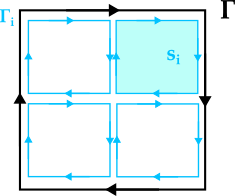
\includegraphics[width=0.38\textwidth]{images/rot} % sostituisci con il nome dell'immagine
\end{wrapfigure}
La definizione $\oint_{C_i} \bold{F} \cdot d \bold{s}$ ha dei problemi nella sua definizione di circuitazione, in quanto l'integrale di linea aumenta all'aumentare della dimensione del circuito nel caso in cui $\bold{F}$ sia costante. Inoltre facendo tendere a zero la superficie $S_i$ racchiusa dal cammino, nel limite puntiforme l'integrale si annulla. Per correggere questa dipendenza dalla geometria del cammino, normalizziamo il circuito rispetto alla superficie $S_i$ che racchiude.
\begin{equation*}
	\frac{1}{S_i} \oint_{C_i} \bold{F} \cdot d\bold{s}
\end{equation*} 
in questo modo si ottiene una buona definizione locale dell'integrale di linea. Tuttavia anche se si perde la dipendenza geometrica rimane la dipendenza dal senso di percorrenza del cammino.
Dato che l'equazione non dipende da una cammino $C_i$ che racchiude una superficie $S_i$ in particolare il segno dell'equazione dipende da come si \`e scelto di suddividere il percorso, mano a mano che si rendono infinitesime le superfici, di conseguenza il passaggio al limite rifletter\`a questa propriet\`a.  Per poter tener conto dell'informazione direzionale introduciamo il vettore $\bold{\hat{n}}$ ortogonale alla superficie infinitesima. 

\begin{wrapfigure}{l}{0.4\textwidth}
    \centering
    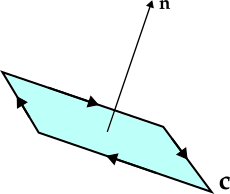
\includegraphics[width=0.38\textwidth]{images/direc} % sostituisci con il nome dell'immagine
\end{wrapfigure}
In questo modo definiamo rotore di un campo vettoriale $\bold{F}$ la grandezza.
\begin{equation}
	\text{rot}\bold{F} \cdot \ \bold{\hat{n}} = \lim_{S_i \to 0} \frac{1}{S_i} \oint_{C_i} \bold{F} \cdot d \bold{s}
\end{equation}
Possiamo domandarci come l'informazione locale che ci viene data dal rotore di un campo si leghi all'integrale di linea del circuito di partenza C da cui siamo partiti. Per rispondere a questa domanda sommiamo tutti i contributi dati che concorrono a formare $C = \sum_i C_i$ 
\begin{equation*}
	\oint_{C} \bold{F} \cdot d \bold{s} = \lim_{\substack{N \to \infty \\[0.2cm] S_i \to 0}} \sum_{i=1}^N \left [\frac{1}{S_i} \oint_{C_i} \bold{F} \cdot d \bold{s} \right ] S_i = \int_S \text{rot}\bold{F}\cdot\bold{\hat{n}}dA = \phi(\text{rot}\bold{F})
\end{equation*}
il risultato
\begin{equation}
	\oint_{C} \bold{F} \cdot d \bold{s} = \int_S \text{rot}\bold{F}\cdot\bold{\hat{n}}dA 
\end{equation}
prende il nome di \textit{teorema di Stokes}. Questo teorema ci dice che la circuitazione di un campo $\bold{F}$ \`e uguale al flusso del rotore di $\bold{F}$ attraverso una qualunque superficie aperta il cui bordo \`e definito dal circuito.

\subsection{Espressione del rotore in coordinate cartesiane}

L'espressione del rotore (1.27) risulta essere poco utile nell'applicazione non dipendendo esplicitamente da un sistema di coordinate. In questo paragrafo esprimiamo il rotore in funzione delle coordinate cartesiane, per farlo prendiamo un punto $\bold{x}_0$ come centro del circuito della faccia giacente nel piano (x,y) di un cubo di volume $dV$ infinitesimo. Possiamo riscrivere l'espressione (1.27) esplicitandone l'integrando di destra 
\begin{equation*}
	\text{rot} \bold{F} \cdot \hat{\bold{n}} = \lim_{S \to 0} \frac{1}{S} \left [ \oint_{C} (F_{y}\text{dy}+F_z\text{dz}) \; +\; \oint_{C} (F_x\text{dx}+F_z\text{dz}) \; + \; \oint_{C}(F_x\text{dz} + F_y\text{dy})\right ]
\end{equation*}
Prendiamo in esame l'ultimo addendo dell'espressione, questo esprime l'integrale di linea di un cammino C giacente nel piano (x,y). 
\newpage

 
\begin{figure}[!ht]
    \begin{minipage}{0.4\textwidth}
        \centering
        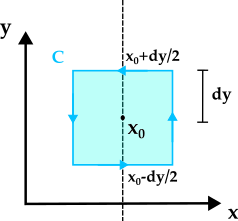
\includegraphics[width=\linewidth]{images/rotar}
    \end{minipage}
   \hspace{2cm}
    \begin{minipage}{0.4\textwidth}
        \centering
        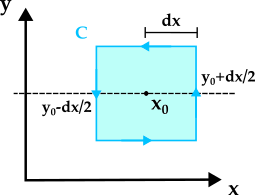
\includegraphics[width=\linewidth]{images/rotar1}
    \end{minipage}
\end{figure}
Utilizzando il teorema della media integrale possiamo esprimerlo come 
\begin{equation*}
	\int_{C_1} F_x dx \simeq F_x(x,y_0-\frac{dy}{2},z)\Delta x  
\end{equation*}
per il cammino $C_1$ inferiore parallelo ad x, mentre per il cammino $C_2$ superiore e parallelo ad x si ha
\begin{equation*}
	-\int_{C_2}F_xdx \simeq F_x(x,y_0+ \frac{dy}{2},z)\Delta x
\end{equation*} 
di conseguenza possiamo riscrivere 
\begin{equation*}
	\frac{1}{\Delta x \Delta y}\int_{C_1+C_2}F_x dx \simeq - \frac{F_x(x,y_0+\frac{dy}{2},z) - F_x(x,y_0-\frac{dy}{2},z)}{\Delta y}
\end{equation*}
facendo il limite per $S \to 0$ si ha che
\begin{equation*}
	\lim_{\Delta x \Delta y \to 0 } \frac{1}{\Delta x \Delta y}\int_{C_1+C_2}F_x dx \simeq \lim_{\Delta y \to 0} - \frac{F_x(x,y_0+\frac{dy}{2},z) - F_x(x,y_0-\frac{dy}{2},z)}{\Delta y} =-\frac{\partial F_x}{\partial y}
\end{equation*}	

Ripentendo lo stesso procedimento per la componente y del campo vettoriale si ha che 
\begin{equation*}
	\lim_{\Delta x \Delta y \to 0} \frac{1}{\Delta x \Delta y} \int_{C_3+C_4}F_y \text{dy} = \lim_{\Delta x \to 0}\frac{F_y(x_0+\frac{dx}{2},y,z) - F_y(x_0-\frac{dx}{2},y,z)}{\Delta x} = \frac{\partial F_y}{\partial x}
\end{equation*}
dunque possiamo concludere che la componente del rotore lungo $\hat{z}$ e dunque ortogonale al circuito \`e data da 
\begin{equation}
	(\text{rot}\bold{F})_z = \oint_{C} (F_x\text{dx}+F_y\text{dy}) = \frac{\partial F_y}{\partial x}-\frac{\partial F_x}{\partial y} 
\end{equation}
 Ripetendo gli stessi procedimenti per le altre direzione del vettore rotore possiamo concludere che 
 \begin{equation*}
 	\text{rot}\bold{F} = \left [ \frac{\partial F_z}{\partial y} - \frac{\partial F_y}{\partial z} \right] \hat{\mu}_{x} + \left [ \frac{\partial F_x}{\partial z} - \frac{\partial F_z}{\partial x}\right] \hat{\mu}_{y} + \left[ \frac{\partial F_y}{\partial x}-\frac{\partial F_x}{\partial y}\right]\hat{\mu}_{z}
 \end{equation*}
\\
\noindent A differenza dell'operazione di gradiente e di divergenza che possono essere definiti su tutto $\mathbb{R}^N$, l'operazione di rotore \`e definita solo per spazi vettoriale in $\mathbb{R}^3$. Possiamo definire l'operazione di rotore utilizzando l'operatore nabla come fatto per la divergenza. In questo avremo che il rotore di un campo $\bold{F} : \mathbb{R}^3 \to \mathbb{R}^3$ \`e esprimibile come 
\begin{equation*}
	\text{rot}\bold{F} = \nabla \times \bold{F}
\end{equation*}  
che definisce ancora un campo vettoriale. Inoltre il rotore pu\`o anche essere espresso come determinante 
\begin{equation*}
	\nabla \times \bold{F} = \text{det}\left [\begin{array}{ccc}
		\bold{e}_1 & \bold{e}_2 & \bold{e}_3 \\
		\frac{\partial}{\partial x} & \frac{\partial }{\partial y} & \frac{\partial}{\partial z}\\
		F_1 & F_2 & F_3
	\end{array}\right ]
\end{equation*}
\noindent Riassumendo abbiamo che la divergenza di un campo vettoriale $\nabla \cdot \bold{F}$ misura il flusso netto del campo attraverso una superficie, mentre il rotore $\nabla \times \bold{F}$ misura la sua rotazione. L'operazione di rotore \`e di fondamentale importanza per determinare se un campo vettoriale pu\`o essere un campo elettrostatico.

\subsection{Propriet\`a del rotore}

Il rotore \`e un operatore differenziale lineare e dunque soddisfa la condizione 
\begin{equation*}
	\nabla \times (\alpha \bold{F} + \bold{G}) = \alpha \nabla \times \bold{F} + \nabla \times \bold{G}
\end{equation*}
per ogni campo vettoriale $\bold{F}$ e $\bold{G}$ e costante $\alpha$. Inoltre gode della propriet\`a di Leibniz 
\begin{equation*}
\begin{aligned}
	& \nabla \times (\phi \bold{F}) = (\nabla \phi) \times \bold{F} + \phi(\nabla \times \bold{F}) \\ 
	& \nabla \cdot (\bold{F} \times \bold{G}) = (\nabla \times \bold{F}) \cdot \bold{G} - \bold{F} \cdot (\nabla \times \bold{G}) 
\end{aligned}
\end{equation*}
dove l'ordine in cui si posizione l'operatore $\nabla$ \`e fondamentale affinch\`e le uguaglianze siano verificate.
\\
Una propriet\`a importante \`e data dal fatto che se ipotizziamo di avere un campo vettoriale $\bold{F}$  conservativo che possiamo esprimere come il gradiente di un campo scalare $\phi$ e ne calcoliamo il rotore, avremo che 
\begin{equation*}
	\nabla \times (\nabla\phi) = 0
\end{equation*}
a patto che $\phi$ soddisfi l'identit\`a di Schwartz, ovvero che sia una funzione  le cui derivate parziali miste sono funzioni continue.

\subsection{Campi conservativi e irrotazionalit\`a}

Sappiamo che un campo vettoriale $\bold{F}$ conservativo pu\`o essere espresso come
\begin{equation*}
	\bold{F} = \nabla \phi
\end{equation*}
per un campo scalare $\phi$. Inoltre un campo vettoriale si dice \textit{irrotazionale} se $\nabla \times \bold{F} = 0$. Per un campo che possiede queste propriet\`a possiamo definire il seguente teorema.
\begin{theorem}
	Per un campo definito ovunque in $\mathbb{R}^3$, essere conservativo \`e equivalente ad essere irrotazionale.
	\begin{equation*}
		\nabla \times \bold{F} \iff \bold{F} = \nabla \phi
	\end{equation*}
\end{theorem}

questo risultano \`e importante in quanto se lo leghiamo al teorema di Stokes dove
\begin{equation*}
	\int_{S}(\nabla \times \bold{F})\cdot \hat{n} = \oint_{C} \bold{F} \cdot d\bold{s}
\end{equation*}
ci permette di concludere che 
\begin{equation*}
	\oint_{C} \bold{F} \cdot d\bold{s} = 0
\end{equation*}
In conclusione nel caso dell'elettrostatica possiamo concludere che un campo vettoriale \`e un campo elettrostatico se e solo se soddisfa il teorema (1.10.1).
\newpage


\section{Equazioni dell'elettrostatica}

\subsection{Operatore Laplaciano}

Il Laplaciano \`e un operatore differenziale del secondo ordine definito da 
\begin{equation*}
	\nabla^2 = \nabla \cdot \nabla = \sum_{i}\frac{\partial^2}{\partial x_i^2}
\end{equation*}
Per esempio su uno spazio vettoriale $\mathbb{R}^3$ il Laplaciano in coordinate cartesiane ha forma
\begin{equation*}
	\nabla^2 = \frac{\partial^2}{\partial x^2} + \frac{\partial^2}{\partial y^2 } + \frac{\partial^2}{\partial z^2}
\end{equation*}
L'operatore Lapalaciano \`e un operatore differenziale scalare, ovvero agisce su campi scalari $\phi$ e restituisce un altro campo scalare $\nabla^2\phi$. Similmente, se agisce componente per componente su un campo vettoriale $\bold{F}$, restituisce un campo vettoriale $\nabla^2\bold{F}$. Se utilizziamo la formula del triplo prodotto scalare si ha 
\begin{equation*}
	\nabla \times (\nabla \times \bold{F}) = \nabla(\nabla \cdot \bold{F} ) - \nabla^2 \bold{F}
\end{equation*}
da cui possiamo ottenere un espressione alternativa del Laplaciano
\begin{equation*}
	\nabla^2 \bold{F} = \nabla(\nabla \cdot \bold{F}) - \nabla \times (\nabla \times \bold{F})
\end{equation*}
\subsection{Equazione di Poisson}

Consideriamo il campo elettrostatico $\bold{E}$ abbiamo visto che localmente la legge di Gauss, per una distribuzioni di carica $\rho$, pu\`o essere espressa rispetto all'operatore gradiente, 
\begin{equation*}
	\nabla \cdot \bold{E} = \frac{\rho}{\varepsilon_0} \quad \text{(Legge di Gauss in forma differenziale)}
\end{equation*}
essendo il campo $\bold{E}$ conservativo pu\`o essere rappresentato come gradiente del potenziale $\bold{E} = - \nabla \phi$, per quanto introdotto con l'operatore Laplaciano, l'espressione della prima equazione di Maxwell assume l'espressione 
\begin{equation}
	\nabla^2\phi = - \frac{\rho}{\varepsilon_0}
\end{equation}
tale equazione di secondo grado alle derivate parziali, prende il nome di \textit{equazione di Poisson}. Nello spazio vettoriale $\mathbb{R}^3$ possiamo esplicitarla come
\begin{equation}
	\frac{\partial^2 \phi}{\partial x^2} + \frac{\partial^2 \phi}{\partial y^2} + \frac{\partial^2 \phi}{\partial z^2} = - \frac{\rho}{\varepsilon_0}
\end{equation}
La soluzio di questa equazione differenziale \`e a noi gi\`a nota, dato che per una distribuzione volumica $\rho$, il potenziale \`e dato dall'equivalenza 
\begin{equation*}
	\phi(\bold{r}) = \frac{1}{4 \pi \varepsilon_0} \int_{V} \frac{\rho(\bold{r'})}{|\bold{r} - \bold{r}'|}dV'
\end{equation*}
Dal punto di vista fisico \`e chiaro che trovare il potenziale elettrostatico tramite la soluzione analitica dell'equazione di Poisson \`e equivalente a calcolare il potenziale per integrazione diretta partendo dal campo $\bold{E}$. In entrambi i gli approcci le espressioni sono state ricavate come conseguenza diretta della legge di Coulomb e del principio di sovrapposizione.

\subsection{Equazione di Laplace}

\begin{wrapfigure}{l}{0.4\textwidth}
    \centering
    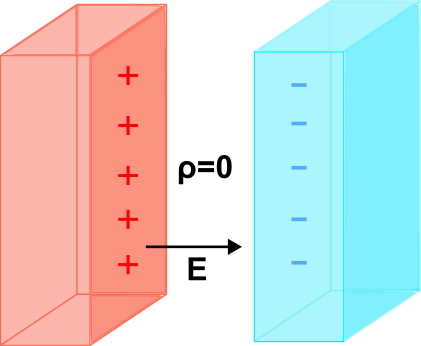
\includegraphics[width=0.38\textwidth]{images/lap} % sostituisci con il nome dell'immagine
    \vspace{0.5cm}
\end{wrapfigure}

Consideriamo un sottocaso dell'equazione di Poisson valide nelle regioni in cui non \`e presente una distribuzione di carica $\rho = 0$. L'equazione di Poisson (1.30) assume la forma 
\begin{equation}
	\nabla^2\phi = 0
\end{equation}

che prende il nome di \textit{equazione di Laplace}.
Questa eqauzione ha soluzione banale per $\phi = 0$, ma soluzioni non banali se si devono soddisfare delle condizioni al contorno; come per esempio in figura. 
\\
Il problema generale dell'elettrostatica consiste proprio nel trovare il potenziale elettrico a partire da una distribuzione $ \rho$, e la sua risoluzione pu\`o essere molte volte ricondotto al cercare una soluzione per l'equazione di Laplace.  

\newpage


\section{Coordinate curvilinee ortogonali}

Fino a questo punto si sono utilizzate le coordiante cartesiane per descrivere gli operatori geadiente, rotazione e divergenza, in questa sezione definiamo degli strumenti matematici che ci permettono di generalizzare questi oggetti per diversi sistemi di coordinate. 
\\

In generale, possiamo descrivere un punto $\bold{x} \in \mathbb{R}^3$ usando le coordinate u,v,w in modo tale che $\bold{x} = \bold{x}(u,v,w)$. Se immaginiamo una variazione infinitesima questa viene descritta dal differenziale del punto
\begin{equation*}
	d\bold{x} = \frac{\partial \bold{x}}{\partial u} du \;+\; \frac{\partial \bold{x}}{\partial v}dv \; + \; \frac{\partial \bold{x}}{\partial w}dw
\end{equation*}
dove ciascuna componente definisce un vettore per le linee di superficie fissate le altre due variabili. Le coordinate (u,v,w) vengono definite \textit{ortogonali e curvilinee} se i vettori tangenti rispettivi sono ortogonali tra loro.
\\

Per delle coordinate curvilinee possiamo sempre definire vettori ortonormali tangenti alle rispettive linee di superficie normalizzandoli. 
\begin{equation*}
	\frac{\partial \bold{x}}{\partial u}=h_u \bold{e}_u \quad,\quad \frac{\partial \bold{x}}{\partial v} = h_v \bold{e}_v \quad , \quad \frac{\partial \bold{x}}{\partial w} = h_w \bold{e}_w
\end{equation*}
dove si sono introdotti i fattori di scala $h_u,h_v,h_w >0$ e i versori $\bold{e}_{v},\bold{e}_{v}$ e $\bold{e}_w$ formano un base ortonormale per cui $\bold{e}_{u} \times \bold{e}_{v} = \bold{e}_{w}$. Possiamo riscrivere il differenziale tenendo conto dei fattori di scala, e dunque
\begin{equation}
	d \mathbf{x}=h_u \mathbf{e}_u d u+h_v \mathbf{e}_v d v+h_w \mathbf{e}_w d w
\end{equation}

\subsubsection{Coordinate cartesiane}
Per le coordinate cartesiane un punto $\bold{x} \in \mathbb{R}^3$ \`e descritto rispetto alle coordinate ortonormali (x,y,z). Se prendiamo il differenziale del punto avremo che l'equazione (1.33) diventa
\begin{equation*}
	d\bold{x} = \text{dx} \; \bold{e}_{x} + \text{dy} \; \bold{e}_{y} + \text{dz} \; \bold{e}_{z}
\end{equation*}
e dunque i fattori di scala sono pari a $h_z = h_y = h_z =1$.

\subsubsection{Coordinate Cilindriche}
Un punto $\bold{x} \in \mathbb{R}^3$ nello spazio \`e descritto dalle coordinate cilindriche rispetto alle variabili $(R\cos\theta,R \sin \theta, z)$ dove $R > 0$ e $\theta \in [0,2\pi]$. L'inversa della trasformazione di coordinate \`e data da 
\begin{equation*}
	R = \sqrt {x^2+y^2} \quad \text{e} \quad \tan \theta = \frac{y}{x}
\end{equation*}

applicando la matrice Jacobiana associata agli elementi della base $\{\bold{e}_1,\bold{e}_2,\bold{e}_3\}$ determiniano la base $\{\bold{e}_{r},\bold{e}_{\theta},\bold{e}_{z}\}$ rispetto al nuovo sistema di coordinate cilindriche 
\begin{equation*}
	\mathcal{J} = \left [ \begin{array}{ccc}
		\cos\theta & -R \sin \theta & 0 \\
		\sin \theta & R \cos \theta & 0 \\
		0 & 0 & 1 
	\end{array} \right ]
\end{equation*}
e dunque 
\begin{equation*}
	\begin{aligned}
& \mathbf{e}_R=\hat{\boldsymbol{R}}=(\cos \theta, \sin \theta, 0) \\
& \mathbf{e}_\theta=\hat{\boldsymbol{\theta}}=(-\sin \theta, \cos \theta, 0) \\
& \mathbf{e}_z=\hat{\mathbf{z}}
\end{aligned}
\end{equation*}
dove 
\begin{equation*}
	h_R = h_z =1 \quad \text{e} \quad h_{\theta} = R
\end{equation*}

\subsubsection{Coordinate Polari}
Per un punto nello spazio definiamo le coordinate sferiche come
\begin{equation*}
	\mathbf{x}=(r \sin \theta \cos \phi, r \sin \theta \sin \phi, r \cos \theta)
\end{equation*}
con $r \geq 0$, $\theta \in [0,\pi]$ e $\phi \in [0,2\pi)$. L'inversa \`e data da
\begin{equation*}
	r=\sqrt{x^2+y^2+z^2} \quad, \quad \tan \theta=\frac{\sqrt{x^2+y^2}}{z} \quad, \quad \tan \phi=\frac{y}{x}
\end{equation*}
Ripetendo quanto fatto per le coordinate cilindriche, la base rispetto alle coordinate sferiche \`e data da
\begin{equation*}
	\begin{aligned}
& \mathbf{e}_r=\hat{\mathbf{r}}=(\sin \theta \cos \phi, \sin \theta \sin \phi, \cos \theta) \\
& \mathbf{e}_\theta=\hat{\boldsymbol{\theta}}=(\cos \theta \cos \phi, \cos \theta \sin \phi,-\sin \theta)\\ 
\end{aligned}
\end{equation*}

\begin{equation*}
 \mathbf{e}_\phi=\hat{\boldsymbol{\phi}}=(-\sin \phi, \cos \phi, 0)	
\end{equation*}
I fattori di scala sono invece dati da
\begin{equation*}
	h_r=1 \quad, \quad h_\theta=r \quad, \quad h_\phi=r \sin \theta
\end{equation*}
Ora che abbiamo definito come cambiano in fattori di scala per diversi sistemi di coordinate, determiniamo la rappresentazione degli operatori visti nelle sezioni precedenti.

\subsection{Gradiente}

L'operatore gradiente \`e uno dei pi\`u semplici da determinare in quanto il differenziale si lega al gradiente di un campo scalare mediante nel seguente modo
\begin{equation*}
	df = \nabla f \cdot d\bold{x}
\end{equation*}
Per un sistema di coordinate generico questa espressione assume la forma esplicita
\begin{equation*}
	d f=\frac{\partial f}{\partial u} d u+\frac{\partial f}{\partial v} d v+\frac{\partial f}{\partial w} d w=\nabla f \cdot\left(h_u \mathbf{e}_u d u+h_v \mathbf{e}_v d v+h_w \mathbf{e}_w d w\right)
\end{equation*}
Usando l'ortonormalit\`a degli elementi della base vettoriale, e comparando i termini di destra con quelli di sinistra possiamo riscrivere il gradiente come 
\begin{equation}
	\nabla f=\frac{1}{h_u} \frac{\partial f}{\partial u} \mathbf{e}_u+\frac{1}{h_v} \frac{\partial f}{\partial v} \mathbf{e}_v+\frac{1}{h_w} \frac{\partial f}{\partial w} \mathbf{e}_w
\end{equation}
Utilizzando i fattori di scala determinati precedentemente abbiamo che il gradiente in coordinate cilindriche per una funzione $f(r,\theta,z)$ \`e 
\begin{equation*}
	\nabla f=\frac{\partial f}{\partial r} \hat{\boldsymbol{r}}+\frac{1}{r} \frac{\partial f}{\partial \theta} \hat{\boldsymbol{\theta}}+\frac{\partial f}{\partial z} \hat{\mathbf{z}}
\end{equation*}
In coordinate polari, il gradiente di una funzione $f(r,\theta,\phi)$ \`e 
\begin{equation*}
	\nabla f=\frac{\partial f}{\partial r} \hat{\mathbf{r}}+\frac{1}{r} \frac{\partial f}{\partial \theta} \hat{\boldsymbol{\theta}}+\frac{1}{r \sin \theta} \frac{\partial f}{\partial \phi} \hat{\boldsymbol{\phi}}
\end{equation*}
\newpage

\subsection{Rotore e Divergenza}

Per costruire gli operatori differenziali di divergenza e rotazione rispetto a delle coordinate generalizzate, definiamo prima l'operatore nabla per delle coordinate generiche 
\begin{equation}
	\nabla=\frac{1}{h_u} \mathbf{e}_u \frac{\partial}{\partial u}+\frac{1}{h_v} \mathbf{e}_v \frac{\partial}{\partial v}+\frac{1}{h_w} \mathbf{e}_w \frac{\partial}{\partial w}
\end{equation}
Dato un campo vettoriale $\bold{F}(u,v,w)$ definito rispetto a delle generiche coordinate ortogonali e curvilinee, la divergenza \`e data da
\begin{equation}
	\nabla \cdot \mathbf{F}=\frac{1}{h_u h_v h_w}\left(\frac{\partial}{\partial u}\left(h_v h_w F_u\right)+\frac{\partial}{\partial v}\left(h_u h_w F_v\right)+\frac{\partial}{\partial w}\left(h_u h_v F_w\right)\right)
\end{equation}
e la rotazione \`e data dal determinante 
\begin{equation}
	\nabla \times \mathbf{F}=\frac{1}{h_u h_v h_w}\left|\begin{array}{ccc}
h_u \mathbf{e}_u & h_v \mathbf{e}_v & h_w \mathbf{e}_w \\
\frac{\partial}{\partial u} & \frac{\partial}{\partial v} & \frac{\partial}{\partial w} \\
h_u F_u & h_v F_v & h_w F_w
\end{array}\right|
\end{equation}
In coordinate cilindriche abbiamo che divergenza e rotore assumono l'espressione
\begin{equation*}
	\begin{aligned}
		&\nabla \cdot \mathbf{F}=\frac{1}{\rho} \frac{\partial\left(\rho F_\rho\right)}{\partial \rho}+\frac{1}{\rho} \frac{\partial F_\phi}{\partial \phi}+\frac{\partial F_z}{\partial z} \\[0.5cm]
		& \nabla \times \mathbf{F}=\left(\frac{1}{\rho} \frac{\partial F_z}{\partial \phi}-\frac{\partial F_\phi}{\partial z}\right) \hat{\boldsymbol{\rho}}+\left(\frac{\partial F_\rho}{\partial z}-\frac{\partial F_z}{\partial \rho}\right) \hat{\boldsymbol{\phi}}+\frac{1}{\rho}\left(\frac{\partial\left(\rho F_\phi\right)}{\partial \rho}-\frac{\partial F_\rho}{\partial \phi}\right) \hat{\mathbf{z}}&
	\end{aligned}
\end{equation*}
mentre per le coordinate sferiche 
\begin{equation*}
	\begin{aligned}
		&\nabla \cdot \mathbf{F}=\frac{1}{r^2} \frac{\partial\left(r^2 F_r\right)}{\partial r}+\frac{1}{r \sin \theta} \frac{\partial\left(\sin \theta F_\theta\right)}{\partial \theta}+\frac{1}{r \sin \theta} \frac{\partial F_\phi}{\partial \phi}\\[0.5cm]
		&\begin{aligned}
\nabla \times \mathbf{F}= & \frac{1}{r \sin \theta}\left(\frac{\partial\left(\sin \theta F_\phi\right)}{\partial \theta}-\frac{\partial F_\theta}{\partial \phi}\right) \hat{\mathbf{r}} +\frac{1}{r}\left(\frac{1}{\sin \theta} \frac{\partial F_r}{\partial \phi}-\frac{\partial\left(r F_\phi\right)}{\partial r}\right) \hat{\boldsymbol{\theta}} 
+\frac{1}{r}\left(\frac{\partial\left(r F_\theta\right)}{\partial r}-\frac{\partial F_r}{\partial \theta}\right) \hat{\boldsymbol{\phi}}
\end{aligned}
	\end{aligned}
\end{equation*}
I risultati (1.35) e (1.36) sono dovuti al fatto che il campo vettoriale deve essere espresso rispetto alla base generalizzata e dunque deve tenere conto dei fattori di scala.
\newpage

\subsection{Laplaciano}

Utilizzando l'espressione (1.34) e (1.36), possiamo esprimere il Laplaciano di un campo scalare per un generico sistema di coordinate come
\begin{equation}
	\nabla^2 f=\nabla \cdot \nabla f=\frac{1}{h_u h_v h_w}\left[\frac{\partial}{\partial u}\left(\frac{h_v h_w}{h_u} \frac{\partial f}{\partial u}\right)+\frac{\partial}{\partial v}\left(\frac{h_u h_w}{h_v} \frac{\partial f}{\partial v}\right)+\frac{\partial}{\partial w}\left(\frac{h_u h_v}{h_w} \frac{\partial f}{\partial w}\right)\right]
\end{equation}
In coordinate cilindriche avremo
\begin{equation*}
	\nabla^2 f=\frac{1}{\rho} \frac{\partial}{\partial \rho}\left(\rho \frac{\partial f}{\partial \rho}\right)+\frac{1}{\rho^2} \frac{\partial^2 f}{\partial \phi^2}+\frac{\partial^2 f}{\partial z^2}
\end{equation*}
mentre in coordinate polari assume la forma 
\begin{equation*}
	\nabla^2 f=\frac{1}{r^2} \frac{\partial}{\partial r}\left(r^2 \frac{\partial f}{\partial r}\right)+\frac{1}{r^2 \sin \theta} \frac{\partial}{\partial \theta}\left(\sin \theta \frac{\partial f}{\partial \theta}\right)+\frac{1}{r^2 \sin ^2 \theta} \frac{\partial^2 f}{\partial \phi^2}
\end{equation*}

\subsection{Esempi ed Esercizi}

\subsubsection{Distribuzioni di carica a simmetria cilindrica}

\begin{wrapfigure}{r}{0.5\textwidth}
  \centering
  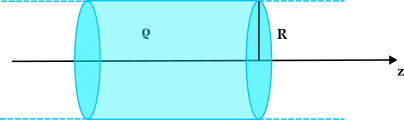
\includegraphics[width=0.5\textwidth]{images/cilindro}
\end{wrapfigure}

Consideriamo una distribuzione di carica $\rho$ per un cilindro di raggio R e lunghezza infinita. Vogliamo calcolarne il campo utilizzando la prima legge di Maxwell.

Per ragioni di simmetria si ha che il campo ha direzione radiale $\bold{E} = E_r(r)\hat{\mu}_r$ e dunque la forma differenziale della legge di Gauss assume la forma 
\begin{equation*}
	\frac{1}{r} \frac{\partial (r E_r)}{\partial r} = \frac{\rho}{\varepsilon_0}
\end{equation*}
risolvendo per quadrature si ha che 
\begin{equation*}
	\bold{E} = \frac{\rho r}{2 \varepsilon_0}\hat{\mu}_{r} +\frac{B}{r}\hat{\mu}_r
\end{equation*}
Per determinare il valore della costante d'integrazione B, possiamo osservare che se misuriamo la forza su una carica $q_0$ nel centro della distribuzione per $r = 0$ si ha che per ragioni di simmetria la forza esercitata \`e $\bold{F} = 0$. Dunque $B=0$.
\\

Dato che all'esterno della distribuzione non \`e presente carica, si ha che 
\begin{equation*}
		\frac{1}{r} \frac{\partial (r E_r)}{\partial r} = 0
\end{equation*}
e dunque 
\begin{equation*}
	\bold{E}_{ext} = \frac{B}{r}
\end{equation*}
utilizzando le condizioni al contorno per la regione cilindrica si ha che 
\begin{equation*}
	\bold{E}_{ext}(r=R) = \bold{E}_{int}(r=R) \iff \frac{\rho R}{2 \varepsilon_0} = \frac{B}{R}
\end{equation*}
e quindi possiamo concludere che 
\begin{equation*}
B = \frac{\rho R^2}{2\varepsilon_0}
\end{equation*}
Il campo complessivamente \`e dato da 
\begin{equation*}
	E(r)= \left \{ \begin{array}{l}
		\frac{\rho r}{2 \varepsilon_0} \quad r \leq R \\
		\frac{\rho R^2}{2 \varepsilon_0} \frac{1}{r} \quad r \geq R
	\end{array} \right.
\end{equation*}
possiamo osservare che il campo esternamente alla distribuzione di carica\`e equivalente a 
\begin{equation*}
	E = \frac{\lambda}{2\pi \varepsilon_0} \frac{1}{r}
\end{equation*}
che \`e quello di un filo infinito con densit\`a di carica lineare $\lambda$.

\subsubsection{Equazione di Poisson per una carica puntiforme}

Consideriamo una densit\`a di carica come una distribuzione
\begin{equation*}
	\rho(\bold{r}) = \delta(\bold{r}) = \left \{ \begin{array}{l}
		0 \quad  \bold{r} > 0 \\
		\neq 0 \quad \bold{r} = 0
	\end{array}\right.
\end{equation*}
dove vale la relazione $\int_{V}\rho dV = q$, per ogni volume che contiene l'origine in cui \`e posta al carica puntiforme q.
Verifichiamo l'equazione di Poisson in due modi:
\begin{enumerate}
	\item In modo esplicito risolvendo l'equazione differenziale $\nabla^2\phi = 0$ per $\bold{r} > 0$
	\item In forma integrale per $\bold{r} \to 0$ usando il teorema della divergenza 
	\begin{equation*}
		\int_{V} \nabla^2\phi dV = -\frac{1}{\varepsilon_0}\int_{V} \delta(\bold{r})dV = -\frac{q}{\varepsilon_0}
	\end{equation*}
\end{enumerate}
1) Siccome il problema \`e a simmetria sferica, consideriamo il Laplaciano in coordinate sferiche e dunque otteniamo l'equazione differenziale
\begin{equation*}
	\nabla^2\phi = \frac{1}{r^2}\frac{\partial }{\partial r} \left (r^2 \frac{\partial \phi}{\partial r} \right) = \frac{q}{4 \pi \varepsilon_0} \frac{1}{r^2} \frac{\partial }{\partial r} \left ( r^2 \frac{\partial}{\partial r} \left ( \frac{1}{r}\right)\right )= 0
\end{equation*}
\\
2)\begin{equation*}
	\int_{V} \nabla^2\phi dV = \int_{V}\nabla \cdot (\nabla \phi) dV = \int_{S}\nabla \phi \cdot d\bold{A}
\end{equation*}
dato che $\nabla^2\phi - 0$ per $\bold{r} \neq 0$, l'unico punto per cui l'integrale \`e non nullo \`e $\bold{r} = 0$. Presa una superficie qualsiasi che racchiude la carica nell'origine abbiamo che
\begin{equation*}
	\int_{S} \nabla \phi \cdot d \bold{A} =  \frac{q}{4 \pi \varepsilon_0}\int_{S} \frac{\partial}{\partial r} \left (\frac{1}{r} \right)\hat{\mu}_{r} \cdot d\bold{A} = - \frac{q}{4 \pi \varepsilon_0} \frac{1}{r^2} (4 \pi r^2)= - \frac{q}{\varepsilon_0} = - \frac{1}{\varepsilon_0}\int_{V} \delta(\bold{r}) dV
\end{equation*} 
e dunque possiamo concludere che 
\begin{equation*}
	\nabla^2\phi = - \frac{\rho}{\varepsilon_0}
\end{equation*}
Dato che abbiamo dimostrato che $\phi = \frac{q}{4 \pi \varepsilon_0} \frac{1}{r}$ \`e la soluzione dell'equazione di Poisson per una carica puntiforme e l'equazione di Poisson \`e lineare, possiamo concludere che la soluzione generale segue dal principio di sovrapposizione.


\section{Conduttori e Isolanti}


Un conduttore \`e una regione di spazio che contiene cariche che sono libere di muoversi. Per esempio i metalli sono tendenzialmente dei buoni conduttori. Come interagiscono questi materiali in presenza di cariche statiche ? a riguardo possiamo trarre le seguenti conclusioni
\begin{itemize}
	\item All'interno di un conduttore il campo elettrostatico $\bold{E} = 0$ \`e nullo
	\item Dato che $\bold{E}  = 0$ all'interno di un conduttore, il potenziale elettrostatico $\phi$ deve essere costante attraverso di esso.
	\item Siccome $\bold{E} = 0$ e vale la prima legge di Maxxwell $\nabla \cdot \bold{E} = \rho  \slash  \varepsilon_0$, si deve vere che $\rho = 0$. Di conseguenza all'interno del conduttore non pu\`o essere presente nessuna carica.
	\item I conduttori possono avere carica neutra, ovvero possiedono carica positiva e negativa che si bilanciano tra loro. Se un conduttore non \`e neutro, e quindi ha un eccesso di carica in uno dei due segni, questa \`e distribuita sulla sua superficie.
	\item Poich\`e $\phi$ \`e costante internamente al conduttore si ha che la superficie che lo racchiude \`e equipotenziale e dunque il campo elettrostatico $\bold{E} = - \nabla \phi$ \`e perpendicolare ad essa.
	\item Se \`e presente della carica di superficie $\sigma $ in qualsiasi parte del conduttore, la discussione della discontinuit\`a del campo insieme al fatto che $\bold{E} = 0$ all'interno, ci dice che il campo elettrico all'esterno del conduttore \`e 
	\begin{equation*}
		\bold{E} = \frac{\sigma}{\varepsilon_0} \hat{\bold{n}}
	\end{equation*}
\end{itemize}

I problemi che interessano i conduttori hanno una natura diversa da quelli affrontati fin'ora. Il motivo \`e che non conosciamo la distribuzione di carica del conduttore in partenza, dunque non possiamo utilizzare gli strumenti precedentemente definiti. Quello che osserviamo sperimentalmente \`e frutto di un interazione con una sorgente di campo $\bold{E}$ esterna che fa s\`i che le cariche interne al conduttore si riorganizzino in modo tale che il campo elettrico interno si annulli con quello esterno 
\begin{equation*}
	\bold{E}_{int} = \bold{E}_{ext} + \bold{E^*}_{int} = 0
\end{equation*}
In generale questo vuol dire che anche conduttori neutri finisco con una distribuzione di carica di superficie, negativa in alcuni punti e positiva in altri, in modo tale che il campo totale interno sia $\bold{E} = 0$.
\newpage
\begin{minipage}{0.5\textwidth}
    \centering
    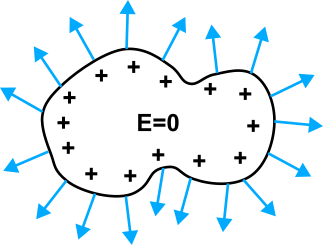
\includegraphics[width=0.8\textwidth]{images/isolanti.png}
    \captionof{figure}{Conduttore carico isolante}
\end{minipage}%
\begin{minipage}{0.5\textwidth}
    \centering
    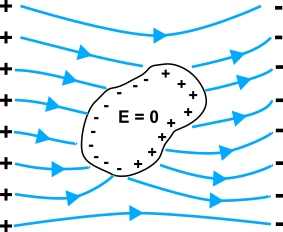
\includegraphics[width=0.8\textwidth]{images/conduct}
    \captionof{figure}{Conduttore neutro }
\end{minipage}
\\

Esistono anche dei materiali che prendono il nome di \textit{isolanti}, questi si elettrizzano facilmente e mantengono indefinitamente il proprio stato di carica. La distinzione tra conduttore ed isolante dipende dal contesto, ovvero dalla scala di tempo del fenomeno rispetto alla scala di tempo del movimento delle cariche. I fattori di risposta dipendono tipicamente dalla temperatura.

\subsubsection{Energia potenziale di una sfera carica di raggio R}

Per una sfera piena si ha che l'energia potenziale configurazionale \`e data da 
\begin{equation*}
	U_c = \frac{Q}{8 \pi \varepsilon_0} \frac{1}{R}
\end{equation*}
mentre per una sfera piena
\begin{equation*}
	U_p = \frac{6}{5} \frac{Q^2}{8 \pi \varepsilon_0} \frac{1}{R}
	\end{equation*}
Dunque in un conduttore a simmetria sferica, la ridistribuzione delle cariche in eccesso sulla superficie  esterna \`e una configurazione energeticamente favorevole, dato che $U_p > U_c$.
In  una sfera la carica di distribuisce in modo uniforme sulla superficie esterna  ( si pu\`o dimostrare che rappresenta la configurazione di minima energia potenziale).
\\
Se il conduttore non \`e sferico la carica si addensa nelle regioni con raggio di curvatura minore, si ha un "effetto punta".
\newpage
\subsubsection{Esempio - Effetto Punta}

Prendiamo un sistema formato da due sfere conduttrici di raggio $R_1 < R_2$ e collegate da un filo. Come si distribuisce la carica sulle rispettive superfici ?
\begin{figure}[!ht]
\vspace{0.2in}
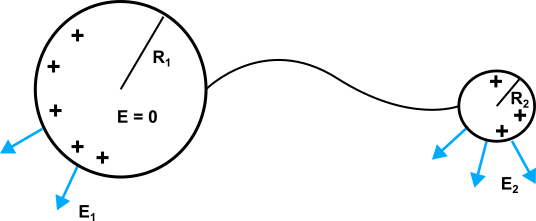
\includegraphics[width = 10cm]{images/punta}	
\centering
\vspace{0.2in}
\end{figure} 

La carica complessiva del sistema \`e data da $Q = Q_1 + Q_2$ dato che le due sfere sono collegate tra loro da un filo e quindi possiamo assumerlo come un sistema unico. Essendo sfere conduttrici internamente il campo $\bold{E} = 0$. Esternamente abbiamo quello di una carica puntiforme e di conseguenza il potenziale \`e dato da
\begin{equation*}
	\phi_1 = \frac{\sigma_1 R_1}{\varepsilon_0} \quad \text{e} \quad \sigma_2 = \frac{\sigma_2 R_2}{\varepsilon_0}
\end{equation*}
Dato che le due sfere conduttrici sono collegate tra loro si trovano allo stesso potenziale e dunque 
\begin{equation}
	\sigma_1R_1 =\sigma_2R_2
\end{equation}
Il risultato (1.39) ci dice che la densit\`a superficiale \`e proporzionale al reciproco del raggio di curvatura, di conseguenza avremo che la carica si addensa maggiormente sulla superficie della sfera con raggio  minore. Possiamo estendere tale risultato a superfici generiche e quindi concludere che, la carica ha densit\`a maggiore laddove il raggio di curvatura \`e il minore possibile.

\subsection{Induzione Totale}

 Consideriamo un sistema isolato in cui \`e presente una sfera conduttrice, in cui \`e presente una cavit\`a contente una carica puntiforme q. Dato che all'interno del conduttore $\bold{E}_{int} = 0$ se consideriamo una superficie Gaussiana che racchiude la cavit\`a per la legge di Gauss si ha che 
 \begin{wrapfigure}{r}{0.5\textwidth}  % 'r' for right, 0.5\textwidth for image width
    \centering
    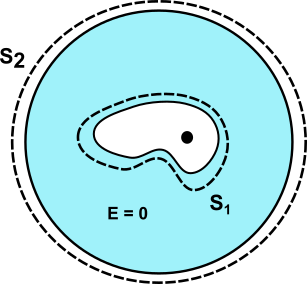
\includegraphics[width=0.46\textwidth]{images/inductor}  % Adjust image width as necessary
\end{wrapfigure}
 \begin{equation*}
 	\frac{1}{\varepsilon_0}\int_{V}dV \; \rho = \int_{S} \bold{E} \cdot d\bold{A} = 0
 \end{equation*}
 e quindi 
 \begin{equation*}
 	Q = q +Q_{int} = 0 \Rightarrow Q_{int} = -q
 \end{equation*}
 Dunque si induce una carica sulla superficie interna della cavit\`a di segno opposto rispetto alla sorgente al suo interno. Se prendiamo una superficie Gaussiana $S_2$ esterna che racchiude il conduttore avremo per la legge di Gauss che 
 \begin{equation*}
 	\int_{S_2}\bold{E} \cdot d\bold{A} = \frac{q}{\varepsilon_0}
 \end{equation*}
 e dunque sulla superficie esterna  avremo una carica
 \begin{equation*}
 	Q_{ext} = q = -Q_{int}
 \end{equation*}
 Per quanto discusso possiamo concludere che per un generico conduttore, la forma del campo elettrico esterno non dipende dalla posizione della carica sorgente posta al suo interno, ma dalla geometria del conduttore stesso. Complessivamente avremo che il campo, per il principio di sovrapposizione \`e dato dai contributi
 \begin{equation*}
 	\bold{E} = \bold{E}_q + \bold{E}_{ind}^{int} + \bold{E}_{ext}^{ind} = \bold{E}_{ext}^{ind}
 \end{equation*}
 dove 
 \begin{equation*}
 	\bold{E}_q + \bold{E}_{ind}^{int} = 0
 \end{equation*}
 dato che la carica sulla superficie esterna \`e distribuita uniformemente. Tale risultato \`e valido per qualsiasi raggio R. 
 Se il conduttore non \`e omogeneo  i risultati sulla carica indotta sono ancora validi solo che il campo esterno non sar\`a pi\`u a simmetria sferica perch\`e la distribuzione di carica non \`e pi\`u uniforme.
 
 \newpage
 
 \subsubsection{Esempio - Induzione con una carica esterna}
 
\begin{figure}[!ht]
\vspace{0.1in}
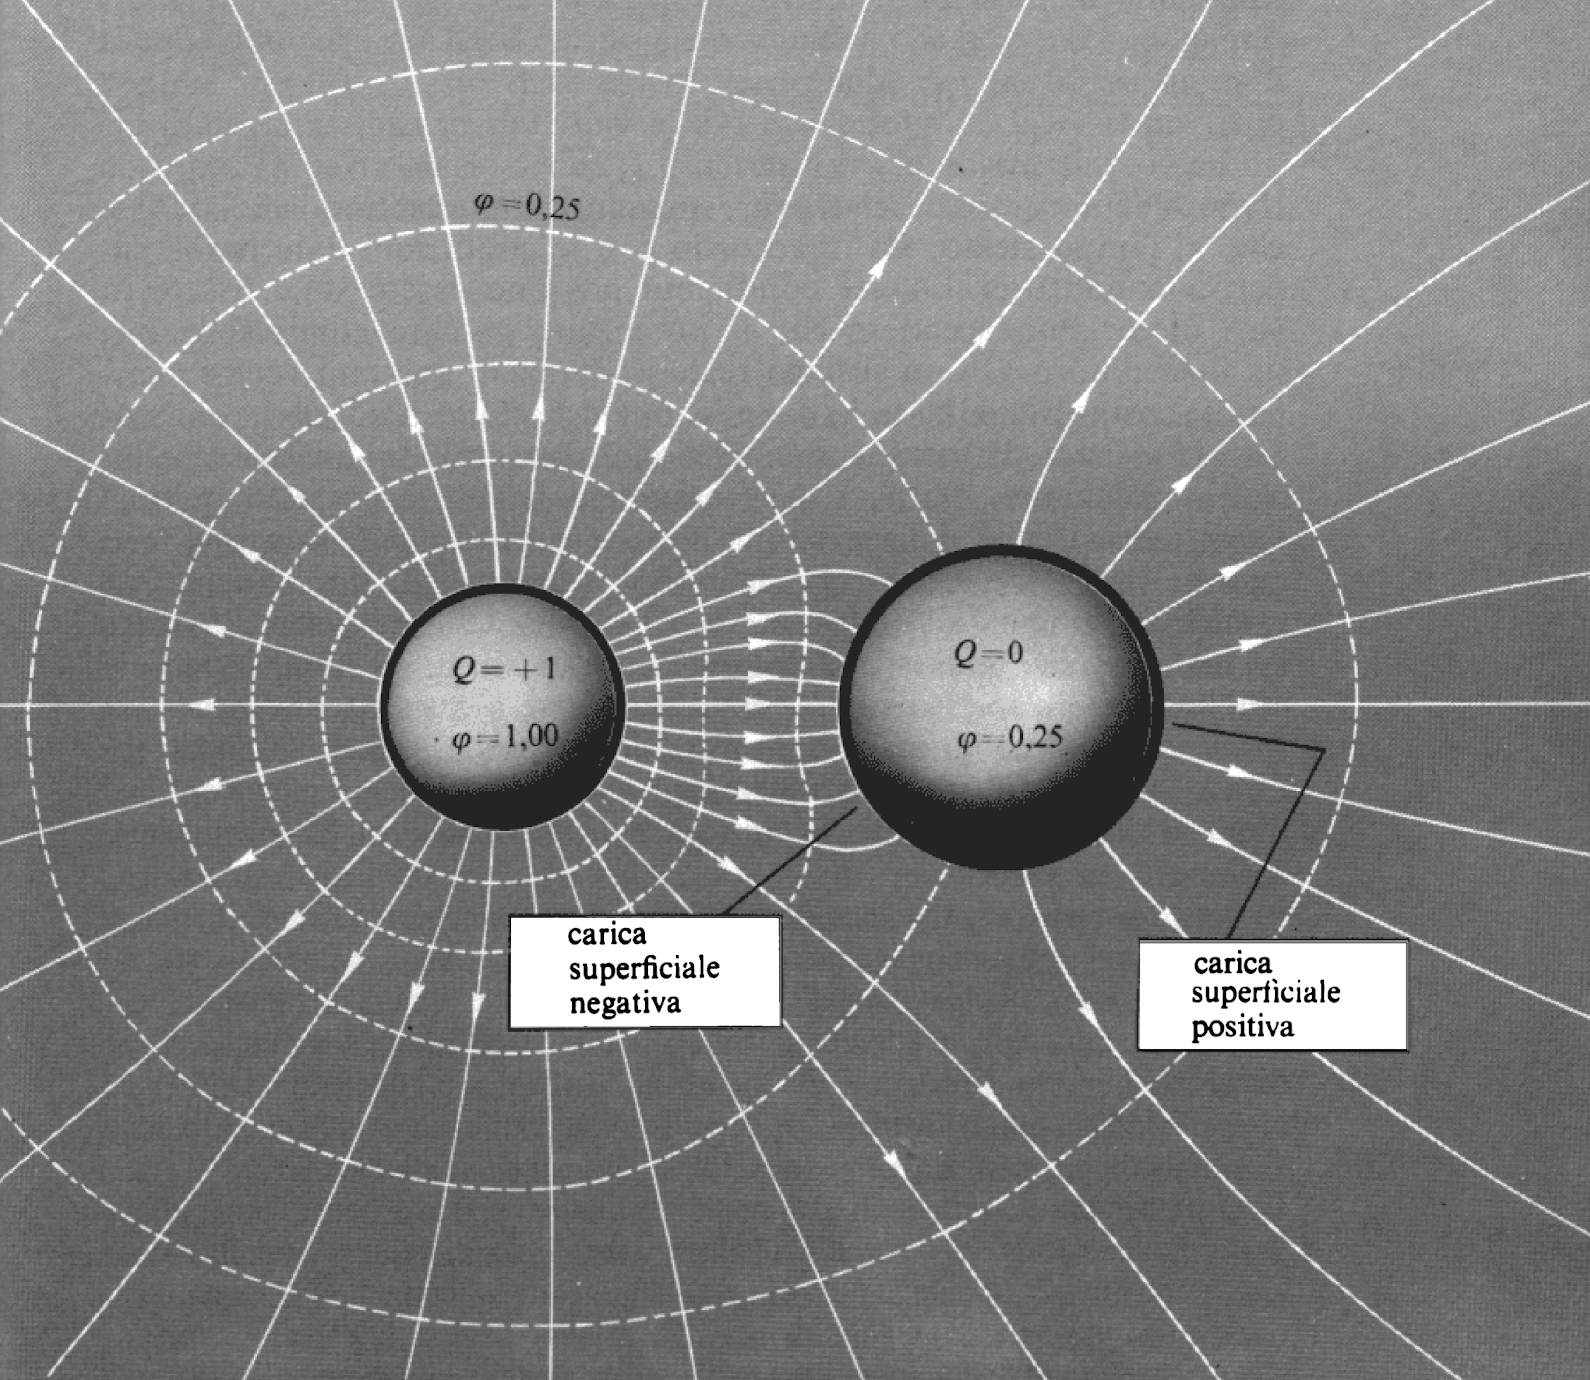
\includegraphics[scale = 0.35]{images/conductor}	
\centering
\vspace{0.1in}
\end{figure}

 Consideriamo una distribuzione di carica a simmetria sferica e un conduttore con la medesima simmetria.
 Avremo che  sul conduttore non possono esserci linee di campo che iniziamo e terminano sulla sua superficie. Per la sorgente di carica le linee di campo sono a simmetria radiale in lontananza. La carica indotta sul conduttore si divide in
 \begin{equation*}
 	Q_{ind} = \left \{ \begin{array}{l}
 		Q > 0 \quad \text{per la superficie interna}\\
 		Q< 0 \quad \text{per la superficie esterna }
 	\end{array}\right.
 \end{equation*}
 Non tutte le linee di campo si possono chiudere sul conduttore, alcune proseguono verso infinito di conseguenza la carica indotta sul conduttore in generale \`e minore di della carica della sorgente.
 \begin{equation*}
 	|Q_{ind}| < |Q|
 \end{equation*}
 Solo quando il conduttore racchiude la carica sorgente possiamo parlare d'induzione totale. 
 \newpage
 
 \subsection{Problema generale dell'elettrostatica: Il teorema di unicit\`a }
 
 Il problema dell'elettrostatica si riduce alla determinazione del campo elettrico a partire da una configurazione di cariche statiche. In linea di principio la soluzione dell'equazione di Maxwell 
 \begin{equation*}
 	\nabla \cdot \bold{E}  = -\frac{\rho}{\varepsilon_0}
 \end{equation*}
 \`e data da 
 \begin{equation*}
 	\bold{E} = \frac{1}{4 \pi \varepsilon_0} \int_{V} dV' \; \frac{\rho(\bold{r}')}{|\bold{r}-\bold{r}'|^2} \hat{u}_{rr'}
 \end{equation*}
 che possiamo ricondurre alla soluzione dell'equazione di Laplace dato che $ \phi = - \nabla \bold{E} $ e quindi
 \begin{equation*}
 	\phi(r) = \frac{1}{4 \pi \varepsilon_0} \int_{V} dV' \; \frac{\rho(\bold{r}')}{|\bold{r}-\bold{r}'|} 
 \end{equation*}
Tuttavia per i problemi che coinvolgono i conduttori la densit\`a di carica $\rho$ non \`e necessariamente nota a priori, per i seguenti motivi:
\begin{enumerate}
	\item La carica si ridistribuisce e in generale per un conduttore conosciamo solo la carica totale di un conduttore, ma non esattamente come \`e distribuita.
	\item Sperimentalmente siamo in grado di determinare solo il potenziale del conduttore.
\end{enumerate}
In questi casi \`e conveniente riformulare il problema , usando le relazioni espresse nelle equazioni di Laplace e Poisson in regioni in cui non \`e presenta della carica libera e rispetto a cui si possono formulare delle condizioni al contorno.

\subsubsection{Esempio}
\begin{wrapfigure}{r}{0.4\textwidth} % 'r' for right, 'l' for left
    \centering
    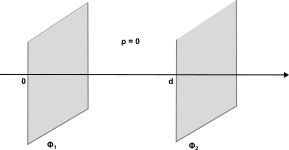
\includegraphics[width=0.4\textwidth]{images/laplacezero} % Replace with your image
\end{wrapfigure}
Prendiamo due piani conduttori infiniti posti in parallelo, nel volume compreso tra i due piani abbiamo carica nulla dunque l'equazione di Laplace \`e 
\begin{equation*}
	\nabla^2 \phi = 0
\end{equation*}
con condizioni al contorno $\phi(0) = \phi_1$ e $\phi(d) = \phi_2$, dove $\phi_2 > \phi_1$. Dato che il campo ha direzione solo lungo l'asse ortogonale ai piani, che consideriamo $x$, l'equazione di Laplace diventa
\begin{equation*}
	\frac{d^2\phi}{dx^2} = 0
\end{equation*}
che ha come soluzione 
\begin{equation*}
	\phi(x) = ax + b
\end{equation*}
Per determinare le costanti $a,b \in \mathbb{R}$, applichiamo le condizioni al contorno, 
\begin{equation*}
	\phi(0) = b = \phi_1 \quad ; \quad \phi(d) = ad+\phi_1 = \phi_2 \Rightarrow a = \frac{\phi_2 - \phi_1}{d}
\end{equation*}

\begin{wrapfigure}{r}{0.4\textwidth} % 'r' for right, 'l' for left
    \centering
    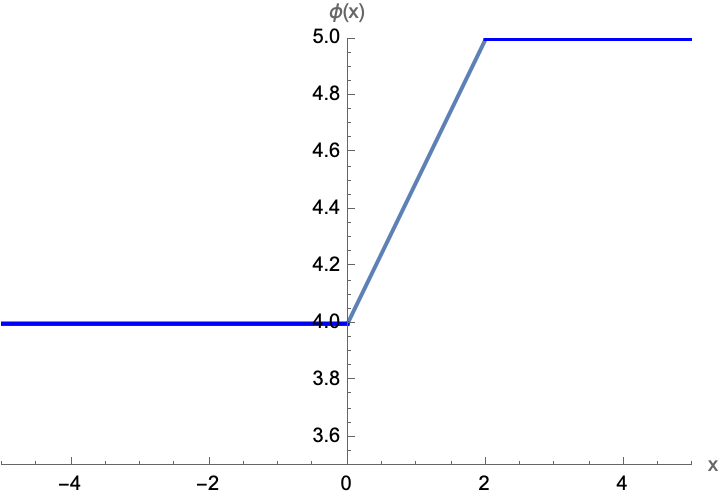
\includegraphics[width=0.4\textwidth]{images/planefield} % Replace with your image
\end{wrapfigure}

quindi il potenziale si comporta nel seguente modo
\begin{equation*}
	\phi(x) = \frac{\phi_2 -\phi_1}{d}x + \phi_1 \quad x \in [0,d]
\end{equation*}

Utilizzando il risultando per cui $\bold{E} = - \nabla  \phi $ abbiamo che il campo elettrico ha la seguente forma 
\begin{equation*}
	\bold{E} = -\frac{(\phi_2 -\phi_1)}{d}\hat{u}_x
\end{equation*}

\noindent I problemi risolti con la metodologia dell'esempio prendono il nome di \textit{problemi confinati}, sono una particolare categoria per cui \`e sempre possibile determinare una soluzione per integrazione. Questo \`e dovuto al fatto che si ha uno spazio chiuso , al cui interno sono presenti regioni di spazio connesse, che contengono della carica e permettono di definire delle condizioni al contorno per l'equazione di Laplace.
\begin{figure}[!ht]
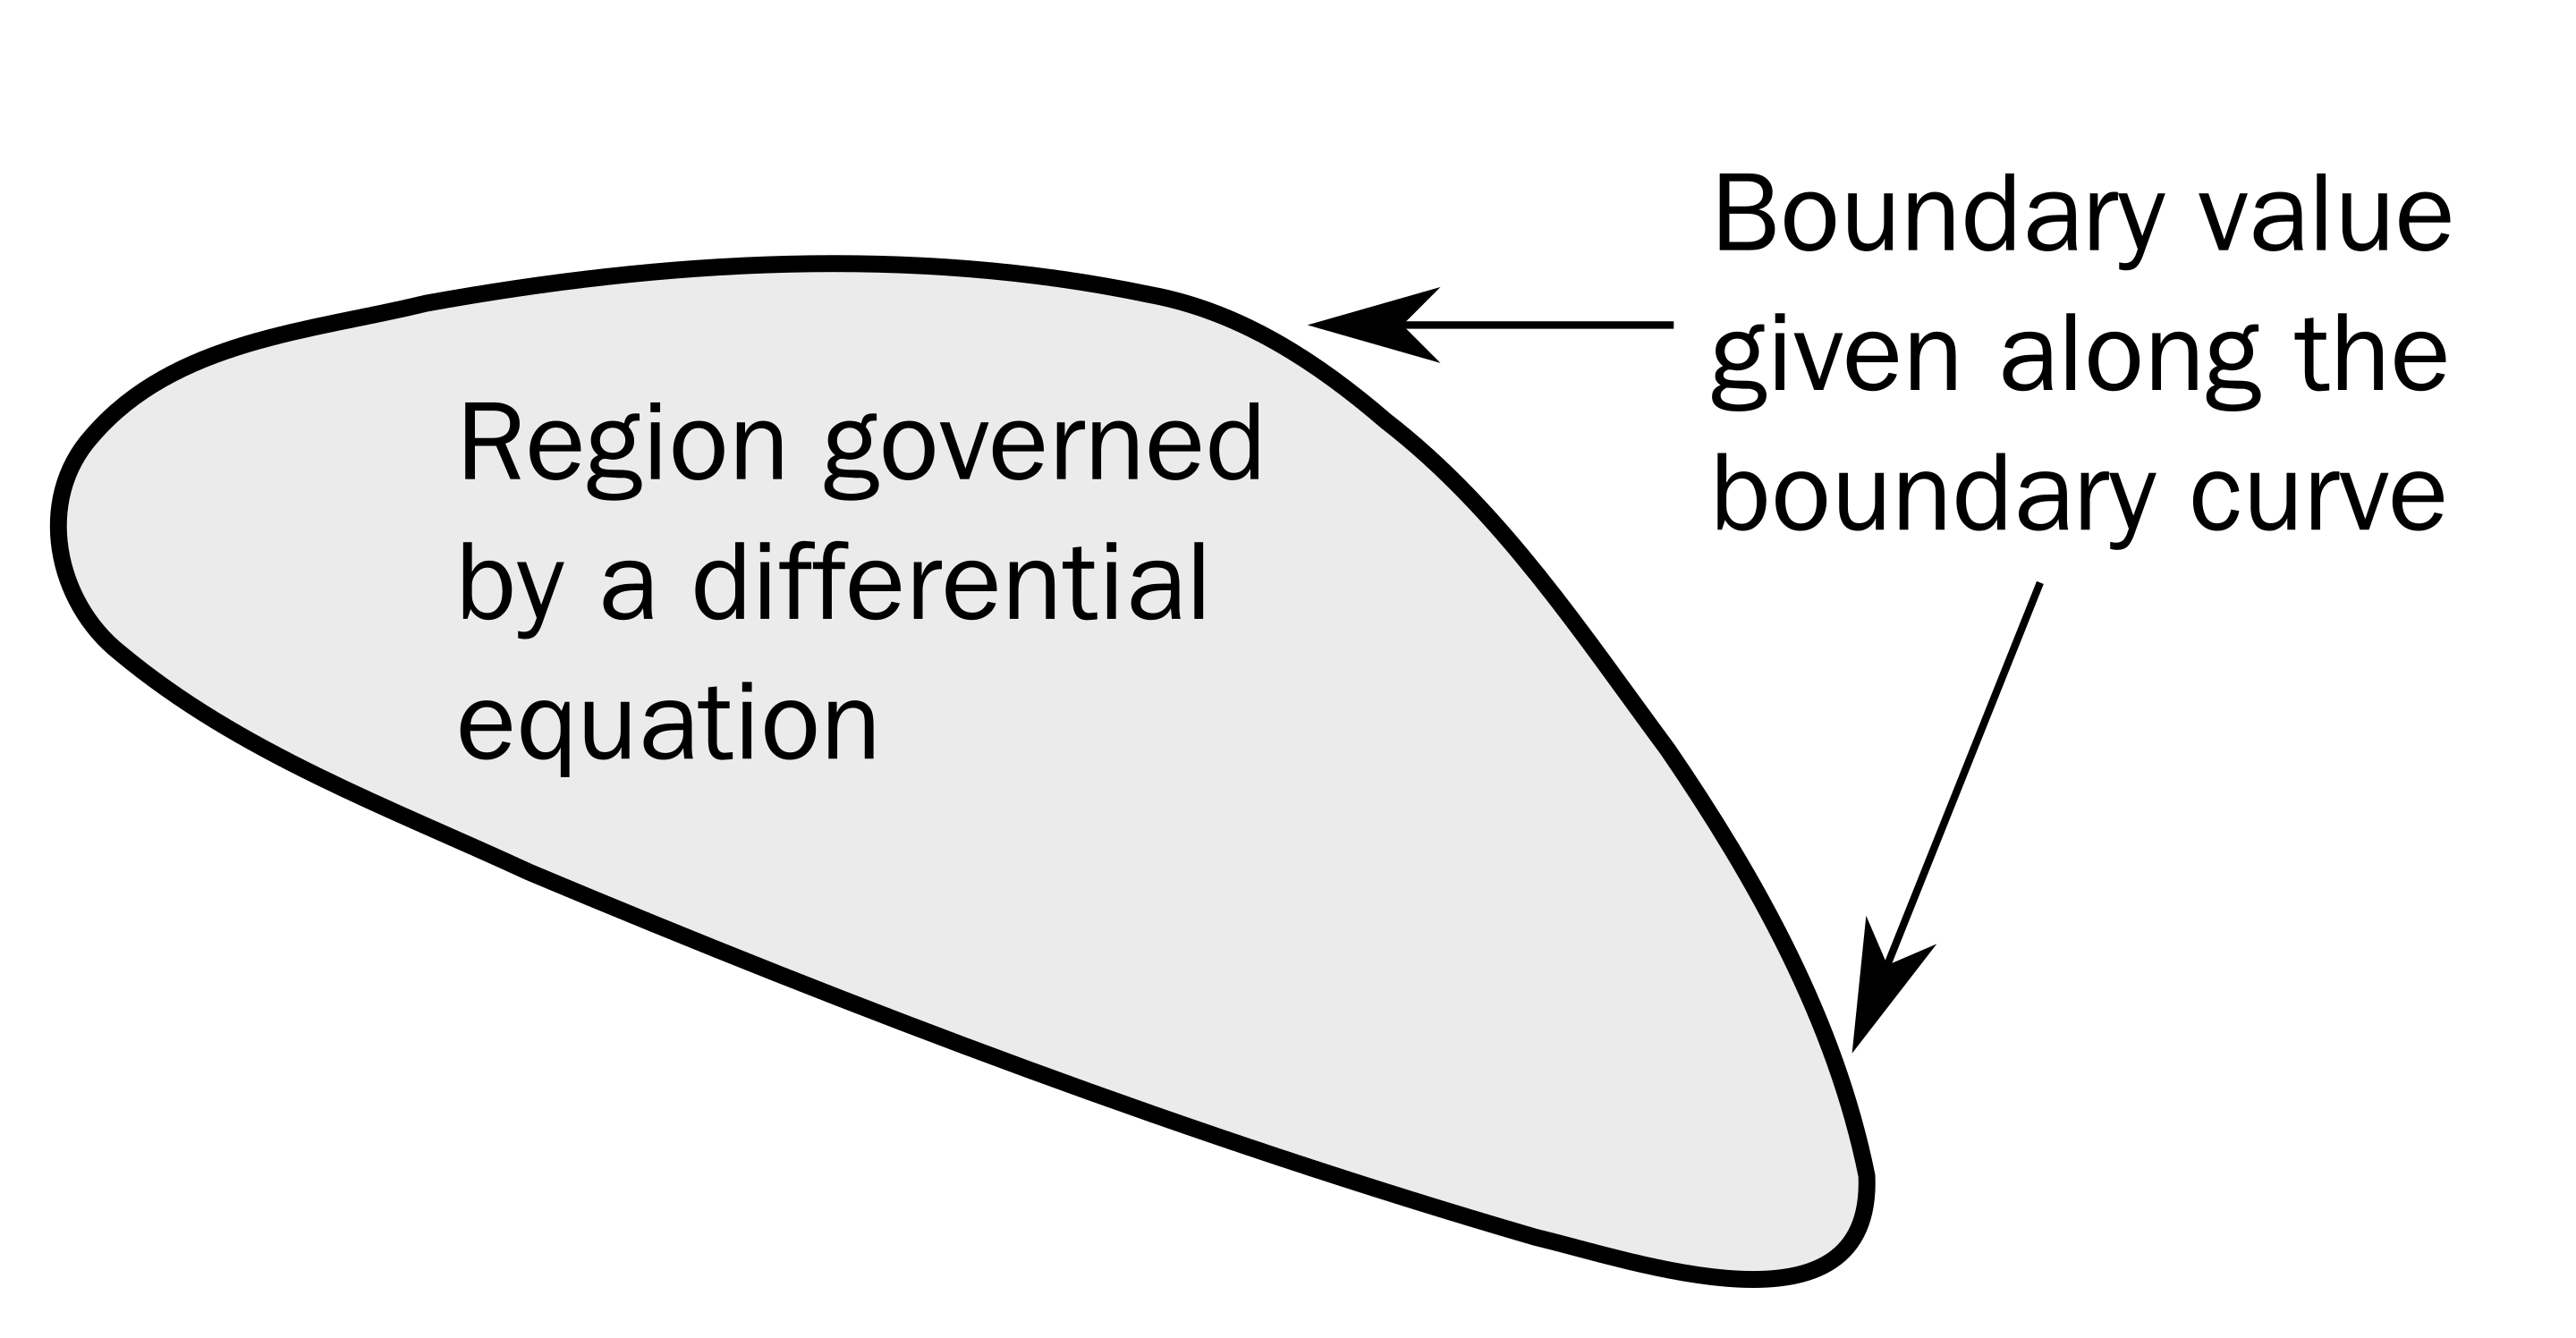
\includegraphics[width = 9cm]{images/boundaryproblem}
\centering
\end{figure}  

\noindent In generale questa tipologia di problemi pu\`o essere risolta utilizzando il metodo di separazione delle variabili.

In generale le soluzioni di questa categoria di problemi, deve soddisfare le seguenti proposizioni:

\begin{prop}
	Il potenziale elettrostatico in un generico punto C \`e uguale al valore medio del potenziale elettrostatico dato da una sfera che ha C come suo centro.
	\begin{equation*}
		\phi_C = \langle \phi_S \rangle 
	\end{equation*}
La seguente propriet\`a risulta essere verficata per tutte le funzioni per cui $\nabla \times \nabla\phi = 0$
\end{prop}
\begin{proof}
	Definiamo 
	\begin{equation*}
		\phi_C = \frac{q}{4\pi\varepsilon_0} \quad \text{e} \quad \langle \phi_S \rangle = \frac{1}{N} \sum_{i=1}^{N} \frac{q'}{4 \pi \varepsilon_0} \frac{1}{r_i} 
	\end{equation*}
Ipotizziamo di volere spostare una carica q ad una distanza r da una carica q' della sfera S, dovremo compiere un lavoro  $W = q \phi'(r) = q'\phi_C(r)$. Ora consideriamo il lavoro per spostare q ad una distanza r, dall'intera sfera, questo \`e dato da 
\begin{equation*}
	W = \frac{1}{N} \sum_{i} \frac{qq'}{4 \pi \varepsilon_0} \frac{1}{r_i} = q \langle \phi_S \rangle 
\end{equation*}
essendo il lavoro il medesimo avremo $\phi_C = \langle \phi_S \rangle $.

\end{proof}
\begin{prop}
	La funzione $\phi$ non possiede valori di estremo nella regione per cui \`e definita l'equazione $\nabla^2 \phi = 0$
\end{prop}
\begin{proof}
	Ipotizziamo per assurdo che esista un punto P nella regione in cui $\nabla^2 \phi = 0$, per cui $\phi(P) = \phi_{max}$ la funzione del potenziale assume valore massimo. Preso un intorno sferico attorno a P, avremo che per tutti i punti appartenenti alla sfera S vale $\phi_S < \phi(P)$, di conseguenza abbiamo un punto di equilibrio del sistema. Il che \`e assurdo perch\`e in una regione di spazio dove \`e definita l'equazione di Laplace non possono esserci configurazioni di equilibrio. (Non \`e vero in generale)
	 
\end{proof}
\begin{prop}
	La  soluzione dell'equazione di Laplace e Poisson \`e unica
\end{prop}
\begin{proof}
	Ipotizziamo che esistano due soluzioni $\phi_1$ e $\phi_2$ dell'equazione $\nabla^2 \phi = 0$ e che siano date le seguenti condizioni al contorno $\phi(\bold{x}_1) = \phi_1,..., \phi(\bold{x}_N) = \phi_N$. Definiamo la funzione $W(x) = \phi_2 - \phi_1$ e di conseguenza le condizioni al contorno diventano $W(\bold{x}_i) = 0$ per $i = 1,..,N$. La funzione W(x) \`e soluzione dell'equazione di Laplace $\nabla^2 W =0$, dato che le condizioni al contorno sono tutte nulle, e dalla propriet\`a precedente W non pu\`o avere punti di massimo e minimo nella regione in cui \`e definita, si deve avere che $W(x) =0 $ ovunque e quindi $\varphi_1	 = \varphi_2$.
	 
\end{proof}


\subsection{Campo all'interno di un conduttore cavo}

\begin{wrapfigure}{r}{0.4\textwidth} % 'r' for right, 'l' for left
    \centering
    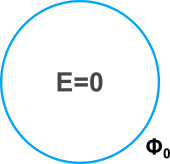
\includegraphics[width=0.3\textwidth]{images/intconduct} % Replace with your image
\end{wrapfigure}
Consideriamo un conduttore chiuso e  cavo (come per esempio un guscio sferico), la sua superficie equipotenziale $\phi_0$ costituisce una condizione al contorno rispetto allo spazio interno in cui si ha l'equazione di Laplace $\nabla^2 \phi =0$. 
La condizione al contorno fa s\`i che la soluzione \`e data da $\phi = k \in \mathbb{R}$, di conseguenza $\bold{E} = - \nabla \phi =0$.
  
\subsection{Metodo delle cariche immagine}

Prendiamo un piano conduttore infinito e poniamo a potenziale nullo $\phi = 0$, e poniamo ad una distanza h una carica puntiforme $q$. Vogliamo descrivere il comportamento del sistema nel suo complesso. 
\begin{figure}[!ht]
\vspace{0.1in}
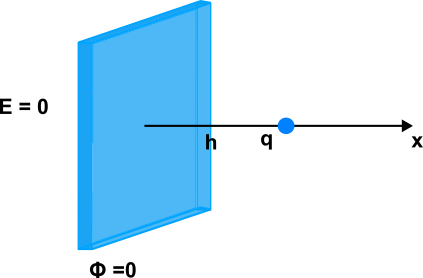
\includegraphics[width = 7cm]{images/chargeplane}	
\centering
\end{figure}

Abbiamo un informazione importante data dal fatto che il piano conduttore \`e messo a terra ovvero ha potenziale nullo. Una configurazione simile in cui si ha un una regione dello spazio in cui il potenziale \`e nullo, la sio ttiene quando si pongono due cariche puntiformi, Q e -Q equidistanziate tra loro, come in figura (1.11)

\begin{figure}[!ht]
\vspace{0.1in}
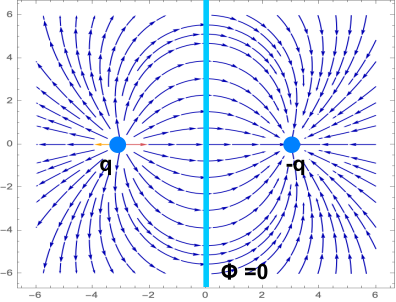
\includegraphics[width = 7cm]{images/imageplane.png}
\centering
\vspace{0.1in}
\caption{}
\end{figure}
Il comportamento del campo magnetico \`e dato dalle linee di campo a sinistra del piano divisore in figura (1.11), ovvero si chiudono sulla superficie, nel caso del problema di partenza, non \`e presente campo $\bold{E} = 0$ in quella parte di spazio divisa dal piano in qui \`e presente la carica $-q$. Vista l'analogia tra i due problemi, poniamo una carica $-q$ in modo simmetricamente opposto ed equidistanziato a q, figura 1.12.
\begin{figure}[!ht]
\vspace{0.1in}
\includegraphics[width = 10cm]{images/mirrormage}
\centering
\vspace{0.1in}
\caption{}
\end{figure}

Il potenziale associato \`e come quello di un dipolo elettrico (nelle prossime sezioni)
\begin{equation}
	\phi(\bold{r})  = \frac{q}{4\pi \varepsilon_0}\left ( \frac{1}{r_+} - \frac{1}{r_-}\right)
\end{equation}
Per tutti i punti in cui $r_+ = r_-$ il potenziale \`e nullo, e coincidono con i punti appartenenti al piano conduttore. Una configurazione di questo tipo ci riconduce al problema di Poisson, dove da una parte \`e presente una distribuzione di carica  e il potenziale sul piano costituisce le condizioni al contorno. Dato che l'equazione ha un unica soluzione, questa coincide con l'equazione (1.40).

Per determinare il valore del campo elettrico sul piano, consideriamo il seguente diagramma delle forze in figura.
\begin{figure}[!ht]
\vspace{0.1in}
\includegraphics[width = 10cm]{images/planechargestudy}
\centering
\vspace{0.1in}
\end{figure}

Le componenti del campo lungo l'asse $\hat{\bold{z}}$ del campo elettrico si annullato. Il campo elettrico lungo $\hat{\bold{x}}$ \`e dato da 
\begin{equation*}
	\bold{E}^{\pm} = -\frac{q}{4\pi \varepsilon_0}\frac{1}{R^2+h^2}\cos \theta \hat{u}_{x} = -\frac{q}{4\pi \varepsilon_0}\frac{h}{(R^2+h^2)^{3/2}} \hat{u}_{x}
\end{equation*}
il campo totale \`e dato da 
\begin{equation*}
	\bold{E} = -\frac{2q}{4 \pi \varepsilon_0} \frac{h}{(h^2 + R^2)^{3/2}} \hat{u}_{z}
\end{equation*}
Dalla legge di Gauss Sappiamo che la distribuzione di carica superficiale $\sigma$ sul piano \`e data da 
\begin{equation*}
	\sigma(R) = - \frac{2q}{4 \pi} \frac{h}{(h^2 + R^2)^{3/2}}
\end{equation*}
Studiando la funzione della distribuzione di carica, si avr\`a una maggiore concentrazione nel centro del piano per R=0.
\begin{figure}[!ht]
\vspace{0.1in}
\includegraphics[width = 8cm]{images/planechagedist}
\centering
\vspace{0.1in}
\end{figure}

\noindent La carica indotta sul piano \`e data da 
\begin{equation*}
	Q_{ind} = \int_{S} \sigma(R) dA
\end{equation*}
dato che la densit\`a di carica dipende dal raggio conviene integrare in coordinate polare sul piano, ovvero $dA = RdRd\theta$, per $\theta \in [0,2\pi]$. L'integrale della carica indotta diventa
\begin{equation*}
	Q_{ind} = -\frac{q}{2 \pi} \int_{0}^{+\infty} \frac{h 2 \pi R}{[R^2+h^2]^{3/2}}dR = -\frac{qh}{2} 
	\Big [-2(R^2+h^2)^{-1/2}\Big ]_{0}^{+\infty} =-q
\end{equation*}
Quindi si ha \textit{induzione totale}, ovvero le linee di campo che escono da $q^+$ si chiudono tutte sul piano.

Abbiamo determinato come si distribuiscono le cariche negative sul piano, ma che cosa succede alle cariche positive?

Mediamente queste non si spostano e sono trascurabili, se consideriamo un disco sul piano, la densit\`a di carica positiva \`e data da 
\begin{equation*}
	\sigma^+ = \frac{q}{2 \pi R^2}
\end{equation*}
se confrontiamo la densit\`a di carica negativa con quella positiva, abbiamo che 
\begin{equation*}
	\frac{\sigma^+}{\sigma^-(0)} = \frac{h^2}{R^2} 
\end{equation*}
se prendiamo $R >> h$, avremo che la carica positiva risulta essere trascurabile. 

Se vogliamo determinare la forza che esercita il piano conduttore sulla carica $q$, questa \`e equivalente alla forza tra due cariche di segno opposto, ovvero
\begin{equation*}
	\bold{F} = q\bold{E} = \frac{q q'}{4\pi \varepsilon_0} \frac{1}{(2h)^2} \hat{u}_{x} = -\frac{q^2}{4 \pi \varepsilon_0} \frac{1}{(2h)^2} \hat{u}_{x}
\end{equation*}
Per determinare l'energia potenziale della configurazione piano-carica, consideriamo l'energia che dovremmo immettere nel sistema per spostare la carica $q$ ad una distanza $h$ dal piano, questa \`e data da 
\begin{equation*}
	U_{piano-q}= W = q\Delta V = -q \int_{h}^{+ \infty} \frac{q}{4\pi \varepsilon_0} \frac{1}{4x^2}dx = \frac{q^2}{4 \pi \varepsilon_0} \frac{1}{4h} = \frac{U_{qq'}}{2}
\end{equation*}
dove l'energia $U_{qq'}$ \`e l'energia d'interazione tra carica immagine $q' = -q$ e $q$. Questa coincide con il lavoro necessario a spostare la carica $q$ ad una distanza $2h$ da $q'$.
\begin{equation*}
	U_{qq'} = -q \int_{2h}^{+\infty} \frac{q'}{4 \pi \varepsilon_0}\frac{1}{x^2}= \frac{qq'}{4 \pi \varepsilon_0}\frac{1}{2h}
\end{equation*}
Il risultato per cui $U_{piano-q} = U_{qq'}/2$ possiamo interpretarlo con il fatto che nella regione di spazio in cui \`e presente la carica immagine il campo elettrostatico \`e nullo, quindi stiamo considerando met\`a del campo dato dall'interazione tra $q$ e $-q$ e quindi anche met\`a dell'energia.

Se allontaniamo la carica sonda $q$ dal piano, la distribuzione di carica negativa formatasi dall'interazione si sparpaglia nel conduttore per mantenere una configurazione in cui il potenziale sul piano \`e nullo. Il lavoro sulle cariche che si spostano all'interno di un conduttore \`e nullo , perch\`e dato $\phi = k \in \mathbb{R}$, allora $W_{cond} = 0$. Possiamo pensare che le cariche si muovano in direzione ortogonale rispetto al campo elettrostatico.

\section{Energia del campo elettrostatico}

Nelle sezioni precedenti abbiamo calcolato l'energia potenziale associata ad una configurazione di cariche. Possiamo vedere una distribuzione di carica continua come un aggregato di tante cariche, che interagiscono tra di loro esercitando una forza di natura Coulombiana e una di coesione, che permette di mantenere la configurazione. Dato che le cariche sono statiche, avremo che 
\begin{equation*}
	\bold{F} = 0 \quad \Rightarrow  \quad q\bold{E} + \bold{F}_{altro} = 0 \quad  \Rightarrow  \quad \bold{F}_{altro} =-q \bold{E}
\end{equation*} 
di conseguenze le forze di coesione avranno pari intensit\`a e direzione, ma verso opposto; inoltre la loro origine \`e di natura elettrica e legata alle cariche atomiche.

Vogliamo dare una definizione alternativa all'energia potenziale elettrostatica calcolando l'energia necessaria ad assemblare la configurazione di carica. 
\newline

\noindent In un certo qual modo pensare di portare delle cariche da infinito tutte insieme e di darle una forma sferica, \`e equivalente ad esercitare contemporaneamente una pressione su tutta una superficie  sferica riducendone uniformemente il raggio. Quindi consideriamo di avere una sfera cava di raggio R e densit\`a di carica superficiale $\sigma $, il campo generale coincide con quello di una carica puntiforme
\begin{equation*}
\bold{E}(r) = \left \{ \begin{array}{l}
	 \frac{1}{4 \pi \varepsilon_0} \frac{\sigma 4 \pi R^2}{r} \hat{u}_{r} \quad r \geq R\\[0.3cm]
	0 \quad r < R
\end{array}\right.
\end{equation*}
e quindi sulla superficie esterna si ha 
\begin{equation*}
	\bold{E} =  \frac{\sigma}{\varepsilon_0} \hat{u}_{r}
\end{equation*}
Le cariche per un area infinitesima $da$ sulla superficie della sfera, esercitano tra di loro una forza di Coulomb 
\begin{equation*}
	d\bold{F} = dq \bold{E}
\end{equation*}
\begin{wrapfigure}{r}{0.4\textwidth} % 'r' for right, 'l' for left
    \centering
    \includegraphics[width=0.4\textwidth]{images/pressure} % Replace with your image
\end{wrapfigure}
Per comprimere la sfera di un tratto $d\bold{r}$, modificandone il raggio bisogna compiere un lavoro sul sistema 
\begin{equation*}
	dU = -dW = -\bold{F} \cdot d\bold{r}
\end{equation*}  
 Le cariche presenti sulla superficie per la sfera con raggio R, si ritroveranno dopo la compressione ad una distanza mediamente inferiore, generando un campo elettrico l\`a dove prima non era presente. Per esprimere dU in funzione del campo elettrico dovuto alla distribuzione delle cariche, abbiamo bisogna di determinare l'espressione della forza $\bold{F}$ d'interazione delle cariche sulla superficie di raggio ridotto.
 
\begin{wrapfigure}{l}{0.4\textwidth} % 'r' for right, 'l' for left
    \centering
    \includegraphics[width=0.4\textwidth]{images/superficie} % Replace with your image
\end{wrapfigure}
Per calcolarla consideriamo uno strato di spesso molto piccolo $d\bold{r}$, equivalente alla quanti\`a di quanto si \`e ridotto il raggio della sfera. Al suo interno \`e presente una densit\`a di carica volumica $\rho$ uniforme e sufficiente affinch\`e si abbia che $ \sigma = \rho dr $ per qualsiasi dr scelto. Si dimostra facilmente usando la legge di Gauss che l'intensit\`a del campo elettrico \`e zero sulla superficie interna dello strato e cresce linearmente fino a raggiungere il valore $4 \pi \sigma $ sulla superficie esterna. 
Il valore medio del campo elettrico nello strato, e di conseguenza la forza media agente su una carica unitaria interna allo strato, \`e 
\begin{equation*}
	\langle E \rangle = \frac{1}{2}(E_{itn} + E_{ext}) = \frac{\sigma}{2\varepsilon_0} 
\end{equation*}
dato che $E_{int} = 0$. La forza agente complessivamente per ogni porzione di superficie $dA$ e larghezza $dr$, sar\`a data dalla relazione 
\begin{equation*}
	F = \int_{o}^{r}dF = \int_{0}^{r}dq \; E = \int_0^r dr\; \rho E da
\end{equation*}
 dove $dq = \rho \cdot da \cdot dr$. Sappiamo che $d\sigma = \rho dr$ utilizzando la legge di Gauss abbiamo deduciamo che $d \sigma = \varepsilon_0 \;dE$, di conseguenza possiamo riscrivere l'integrale precedente rispetto al campo elettrico
 \begin{equation*}
 	P = \frac{F}{da} = \varepsilon_0 \int_{E_{int}}^{E_{ext}} dE \; E = \frac{1}{2} \varepsilon_0 (E_{ext}^2-E_{int}^2) = \frac{1}{2} \varepsilon_0(E_{ext} + E_{int})\Delta E
 \end{equation*}
 dove $\Delta E = \sigma / \varepsilon_0$ e quindi possiamo concludere che la \textit{pressione elettrostatica} \`e data da 
 \begin{equation*}
 	P = \frac{\sigma^2}{2 \varepsilon_0}
 \end{equation*}
 La direzione della forza \`e verso l'esterno della superficie, indipendentemente dal segno della carica dato che \`e quadratica nell'espressione.
 
 Dalla pressione possiamo determinare la densit\`a di energia elettrostatica immagazzinata all'interno del volume $dV = 4\pi R^2 dr$, dato che 
 \begin{equation*}
 	dU = - \bold{F} \cdot d \bold{r} = \frac{\sigma^2}{\varepsilon_0} 4 \pi R^2dr
 \end{equation*}
 che possiamo riscrivere come 
 \begin{equation*}
	dU = \frac{1}{2} \varepsilon_0 E^2 (4\pi R^2dr) \quad \Rightarrow  	u_e = \frac{dU}{dV} = \frac{1}{2}\varepsilon_0 E^2
 \end{equation*}
Ora che abbiamo determinare la quantit\`a di energia presente per unit\`a di volume nello spazio, possiamo calcolare l'energia, integrando sul volume, e quindi definiamo
\begin{equation}
	U = \frac{1}{2} \varepsilon_0 \int_{V} d\nu \; E^2
\end{equation}

\section{Dipolo elettrico}

Un \textit{dipolo} consiste in un sistema di due cariche Q e -Q poste a una distanza $d$. La prima carica \`e posizionata in $d/2$ e la seconda in $-d/2$. Il potenziale non \`e altro che la somma dei potenziali di ciascuna carica
\begin{equation*}
	\phi(r) = \frac{Q}{4 \pi \varepsilon_0} \left( \frac{1}{r_1} - \frac{1}{r_2}\right)
\end{equation*}
Prendiamo un punto P nello spazio  affinch\`e la sua distanza radiale $r$ sia molto pi\`u grande della distanza tra le due cariche. Riscriviamo le congiungenti tra le cariche e P rispetto ad $r$ nel seguente modo
\begin{equation*}
	r_1 = r + \frac{d}{2}\cos\theta \quad \text{e} \quad
	r_2 = r - \frac{d}{2}\cos \theta 
\end{equation*} 
l'espressione del potenziale diventa 
\begin{equation*}
	\phi(r) = \frac{Q}{4 \pi \varepsilon_0} \left(\frac{1}{r + d/2 \cos\theta } - \frac{1}{r - d/2 \cos\theta} \right) = \frac{Q}{4 \pi \varepsilon_0} \frac{d \cos \theta }{r^2 - d^2/4\cos \theta}\simeq \frac{Qd}{4 \pi \varepsilon_0} \frac{ \cos \theta }{r^2}
\end{equation*}
dato che siamo sotto l'ipotesi in cui $r >> d$ si \`e sviluppato in potenziale con Taylor arrestandosi al primo ordine .
Alcune osservazioni:
\begin{enumerate}

\item Nel potenziale compare il termine $ p=Qd$ che prende il nome di \textit{momento di dipolo}.

\item Un dipolo ideale \`e dato da $d \to 0$ e $q \to \infty $ con il momento di dipolo che assume un particolare valore finito. A differenza del potenziale di una carica puntiforme quello del dipolo \`e proporzionale a $1/r^2$ decrescendo molto pi\`u velocemente; questo \`e dovuto al fatto che il potenziale delle due cariche opposte tende a cancellarsi quando $r >> d$. L'unico contributo restante \`e quello dovuto alla distanza tra due cariche leggermente differenti.
\item Il potenziale \`e proporzionale al $\cos \theta $, questo ci dice che in direzione $\perp$ al dipolo il potenziale \`e $\phi(r,\pm \pi/2) = 0$, mentre per una direzione parallela il potenziale \`e massimo.

\end{enumerate}

Utilizzando le coordinate sferiche per l'operatore gradiente determininato il campo elettrostatico generato dalla configurazione di carica
\begin{equation*}
	\bold{E} = -\nabla \phi = - \left [ \frac{\partial \phi }{\partial r}\hat{u}_r + \frac{1}{r} \frac{\partial \phi}{\partial \theta}\hat{u}_{\theta} \right ] = \frac{Qd}{4 \pi \varepsilon_0}\frac{1}{r^3} [2 \cos \theta \hat{u}_{r} + \sin\theta \hat{u}_{\theta}]
\end{equation*}

 
\begin{figure}[!ht]
\vspace{0.1in}
\includegraphics[width = 8cm]{images/dipol1}	
\centering
\caption{Campo elettrico generato da un dipolo}
\end{figure}

\newpage

\section{Esempi ed esercizi}

\subsection{Carica puntiforme in prossimit\`a di una sfera conduttrice (Esame 23/06/2020)}

\begin{wrapfigure}{r}{0.4\textwidth} % 'r' for right, 'l' for left
    \centering
    \includegraphics[width=0.4\textwidth]{images/spherecharge} % Replace with your image
\end{wrapfigure}
Si consideri un sistema dove si ha una carica puntiforme $q$ ad una distanza $a$ da un conduttore sferico con massa a terra di raggio $r$. Vogliamo calcolare il lavoro necessario ad allontanare la carica da $a$, verso infinito.

\begin{proof}
	Per risolvere il problema possiamo usare il metodo della carica immagine, ovvero andiamo a collocare una carica immaginaria $Q$ all'interno del conduttore, affinch\`e il potenziale $\phi$ sulla superficie della sfera sia nullo. Di conseguenza abbiamo bisogno di determinare per quali valori $Q$ e in quale posizione $x$ tale condizione \`e verificata.
\newline

Ipotizziamo si posizionare le due cariche $Q$ e $q$ in due generici punti $(b,0,0)$ dove $b < r$ e $(a,0,0)$ per $a >r$. Il potenziale complessivo del sistema a due cariche \`e dato da 
\begin{equation*}
	V(x,y,z) = \frac{1}{4 \pi \varepsilon_0} \left [ \frac{q}{\sqrt{(x-a)^2 + y^2 + z^2}} + \frac{Q}{\sqrt{(x-b)^2+y^2+z^2}} \right]
\end{equation*}
Imponendo la condizione $\phi = 0$, abbiamo che 
\begin{align*}
	& \frac{q}{\sqrt{(x-a)^2 + y^2 + z^2}} =- \frac{Q}{\sqrt{(x-b)^2+y^2+z^2}} \iff \frac{Q^2}{q^2} = \frac{(x-b)^2 + y^2 + z^2}{(x-a)^2 + y^2 + z^2} \\[0.5cm]
	& \Rightarrow \frac{Q^2}{q^2} = \frac{x^2 + y^2 +z^2 +2bx + b^2}{x^2 + y^2 +z^2 + 2ax + a^2} = \frac{r^2 - 2bx +b^2}{r^2 - 2ax +a^2} 
	\Rightarrow \\[0.5cm]
	& \Rightarrow \frac{Q^2}{q^2}r^2 + \frac{Q^2}{q^2}a^2 - 2\frac{Q^2}{q^2}ax =  r^2 - 2bx +b^2 \Rightarrow 
\end{align*}
\begin{align}
	& \Rightarrow r^2 \left( \frac{Q^2}{q^2}-1 \right) = -\frac{Q^2}{q^2}a^2 +b^2 + 2x \left(\frac{Q^2}{q^2}a - b\right)
\end{align}
l'equazione (1.42) assume un espressione semplifica se poniamo l'ultimo addendo nullo, ovvero $b = (Q^2/q^2)a$, e quindi possiamo riscrivere l'equazione nel seguente modo:
\begin{equation*}
	r^2 \left( \frac{b}{a} -1\right) = -ab + b^2  = ab\left (\frac{b}{a}-1 \right) \Rightarrow r^2 = ab
\end{equation*}
troviamo dunque che la posizione della carica Q affinch\`e $\phi(x,y,z) = 0$ \`e data  da 
\begin{equation*}
\boxed{
	b = \frac{r^2}{a}
	}
\end{equation*}
ci manca ora da determinare la carica immagine $Q$  all'interno del conduttore sferico affinch\`e $\phi(R) = 0$. Per farlo riscriviamo l'espressione del potenziale complessivo con il risultato trovato,
\begin{equation*}
	\phi(x,y,z) = \frac{1}{4 \pi \varepsilon_0} \left [ \frac{q}{\sqrt{(x-a)^2+y^2+z^2}} + \frac{Q}{\sqrt{(x-r^2/a)^2 +y^2+z^2}}\right]
\end{equation*}
e imponiamo che per $\phi(r,0,0) = 0$  e quindi abbiamo l'equazione 
\begin{equation*}
	\phi(r) = \frac{1}{4 \pi \varepsilon_0} \left [ \frac{q}{|r-a|} + \frac{Q}{|r - \frac{r^2}{a}|}\right] = 0
\end{equation*}
dato che $a >R$ si ha che $|r-a| = -(r-a)$.L'equazione diventa
\begin{align*}
	& Q = \frac{q}{r-a}\left ( r-\frac{r^2}{a}\right)\\[0.5cm] 
	& \Rightarrow \boxed{Q = -\frac{r}{a}q}
\end{align*}
dunque per un potenziale del seguente tipo 
\begin{equation*}
	V(x,y,z) = \frac{q}{4 \pi \varepsilon_0} \left [ \frac{1}{\sqrt{(x-a)^2 +y^2 + z^2}} - \frac{r}{a}\frac{1}{\sqrt{(x- r^2/a)^2+y^2 +z^2}}\right]
\end{equation*}
abbiamo che \`e soddisfatta la condizione che $\phi(r) = 0$.

Infine possiamo rispondere alla domanda dell'esercizio dove il lavoro per muovere una carica puntiforme da $a$ ad $\infty$ \`e dato da
\begin{equation*}
	W = q \phi(a) = \frac{q^2}{4 \pi \varepsilon_0} \frac{r}{a^2-r^2} 
\end{equation*}
siccome all'interno della sfera conduttrice non c'\`e campo, per il sistema originale dobbiamo considerare met\`a dell'energia trovata e quindi
\begin{equation*}
	W' = \frac{1}{2}W = \frac{q^2}{4 \pi \varepsilon_0} \frac{r}{a^2-r^2}
\end{equation*}

\end{proof}

Che cosa succede se consideriamo la sfera conduttrice scarica e la rimuoviamo dalla messa a terra ?

 \begin{wrapfigure}{l}{0.4\textwidth} % 'r' for right, 'l' for left
    \centering
    \includegraphics[width=0.3\textwidth]{images/spherecharge1} % Replace with your image
\end{wrapfigure}

Avremo che sulla superficie della sfera si crea una distribuzione uniforme di carica $Q'' = -Q$ tale per cui la carica netta su di essa \`e $Q' = Q + Q'' = 0 $ e quindi il conduttore sferico \`e neutro. Questo equivale a porre una seconda carica immagine $Q''$ al centro della sfera. 

Applicando il principio di sovrapposizione per il potenziale di ciascuna carica e considerando l'orgine del sistema di riferimento con il centro della sfera, avremo che 
\begin{equation*}
	\phi(x,y,z) = \frac{q}{4 \pi \varepsilon_0} \left [ \frac{1}{\sqrt{(x-r)^2 + y^2 +z^2}} - \frac{R}{r}\frac{1}{\sqrt{(x-R^2/r)^2 + y^2 + z^2}} + \frac{R}{r} \frac{1}{\sqrt{x^2+y^2+z^2}}\right]
\end{equation*}
Per determinare il lavoro necessario a spostare la carica da $r$ a $+ \infty$ calcoliamo
\begin{equation*}
	W = q\phi(r,0,0) = \frac{q^2R}{4 \pi \varepsilon_0} \left(\frac{1}{r^2-R^2} - \frac{1}{r^2} \right)
\end{equation*}
l'energia trovata \`e quella della configurazione delle cariche, per determinare quella associata alla sfera conduttrice neutra, dobbiamo ricordare che internamente il campo \`e nullo e dunque il lavoro necessario \`e la met\`a di W.
\begin{equation*}
	W' = W/2 = \frac{q^2R}{8 \pi \varepsilon_0} \left(\frac{1}{r^2-R^2} - \frac{1}{r^2} \right)
\end{equation*}

\subsection{Esercizio 2}












	\setcounter{chapter}{1}
\chapter{Magnetostatica}

\section{Correnti stazionarie}

Le cariche generano campi elettrici. Le correnti di cariche generano campi magnetici. Restringiamo lo studio al caso in cui la densit\`a di carica \`e $\rho = 0$, in modo tale che $\bold{E} = 0$ e quindi possiamo concentrarci solo sul campo magnetico. 

Dato che per ipotesi $\rho = 0$, non pu\`o esserci carica netta, questo vuol dire che cariche positivi e negative si bilanciano tra loro in ogni punto dello spazio. Inoltre, dato che le cariche possono muoversi \`e presente una corrente anche se non c'\`e un trasporto netto di carica.
\newline

Sembrer\`a strano, ma \`e esattamente quello che succede all'interno di un normalissimo filo. Questo \`e dovuto al fatto che ci sono delle cariche positive libere nel metallo per via del reticolo di ioni, ma dato che si muovono tutti insieme riusciamo ad avere in ogni singolo punto una densit\`a di carica nulla. L'\textit{equazione di continuit\`a}, che descrive la conservazione della carica \`e data da, 
\begin{equation}
	\frac{\partial \rho}{\partial t} + \nabla \cdot \bold{J} = 0
\end{equation}
e dato che la densit\`a di carica \`e costante, diventa 
\begin{equation*}
	\nabla \cdot \bold{J} = 0
\end{equation*}
Matematicamente vuol dire che se abbiamo un flusso di corrente in una certa regione di spazio, un eguale corrente deve fluire in senso opposto affinch\`e non ci sia un addensamento di carica. Notare che questo \`e consistente con la propriet\`a che per ogni campo vettoriale si ha che $\nabla \cdot (\nabla \times \bold{B}) = 0$.

\subsection{Derivzione dell'equazione di continuit\`a}

Per caratterizzare il trasporto di carica si introducono alcune grandezze fisiche. Una delle prime \`e \textit{l'intensit\`a di corrente:}
\begin{equation*}
	I = \frac{dq}{dt}
\end{equation*} 
che descrive la quantit\`a di carica netta che attraversa ala sezione di un mezzo in unit\`a di tempo. La unit\`a di misura in cui viene espressa \`e data dall`\textit{Ampere} che esprimiamo come
\begin{equation*}
	[A] = \frac{[ Coulomb]}{[ Secondi]}
\end{equation*}
La definizione pu\`o essere generalizzata al trasporto di carica nello spazio, riconducendola ad una grandezza vettoriale e al concetto di flusso attraverso una superficie.
\begin{wrapfigure}{r}{0.4\textwidth}  % r for right alignment, 0.4 is the width of the figure
    \centering
    \includegraphics[width=0.4\textwidth]{images/fluxden}  % Include your image here
\end{wrapfigure}

La seconda grandezza che andiamo ad introdurre \`e la \textit{densit\`a di corrente}, questa \`e legata ad un volume generico costituito da un materiale al cui interno le cariche siano libere di muoversi in una direzione generica. Ipotizziamo di avere nel mezzo dei portatori di carica tutti identici tra loro, identificati dalle seguenti grandezze comuni:

\begin{enumerate}
	\item $n_q \rightarrow$ densit\`a di portatori di carica per unit\`a di volume ;
	\item $q \rightarrow $ carica dei portatori;
	\item $\bold{v} \rightarrow $ velocit\`a di spostamento delle cariche;
	\item $\bold{da} \rightarrow$  elemento infinitesimo di superficie del volume.  
\end{enumerate} 
Dato il parallelepipedo in figura solo le cariche al suo interno di base $da$ e altezza $h = v \Delta t \cos \theta $ attraversano la superficie in un intervallo di tempo $\Delta t$.

Di conseguenza la variazione di carica attraverso la superficie $\bold{da}$ \`e data dalla relazione 
\begin{equation*}
	\Delta Q = n \;q\; da \; h = n\; q \;v \Delta t \cos \theta da = n \;q \; \bold{v} \cdot \bold{da} \; \Delta t 
\end{equation*}
La corrente attraverso $\bold{da}$ \`e associata al flusso della grandezza $n_q \bold{v}$, da cui possiamo definire 
\begin{equation*}
	dI = \lim_{\Delta t \to 0} \frac{\Delta Q}{\Delta t} = nq \bold{v} \cdot \bold{da} 
\end{equation*}
Nel caso pi\`u generico all'interno del volume possono esistere diversi portatori di carica $q_i$, con velocit\`a differenti $\bold{v}_i$, dunque per ciascuna specie di particella possiamo definire 
\begin{equation*}
	dI_i = (n_iq_i\bold{v}_i)\cdot \bold{da}
\end{equation*}
e di conseguenza la corrente infinitesima complessiva \`e 
\begin{equation*}
	dI = \sum_{i}dI_i = \left (\sum_{i}n_i q_i \bold{v}_i \right) \cdot \bold{da}
\end{equation*}
dove definiamo la grandezza vettoriale
\begin{equation*}
	\bold{J}= \sum_{i}n_i q_i \bold{v}_i 
\end{equation*}
\textit{densit\`a di corrente}, che \`e identificata dalle unit\`a di misura 
\begin{equation*}
	[\bold{J}] = [I \; L^{-2}] = \frac{Ampere}{m^2}
\end{equation*}
Non \`e necessario che tutte le cariche dello stesso tipo abbiamo la medesima velocit\`a $\bold{v}_i$. In un conduttore tipico, $\bold{v}_i$ \`e definita da una distribuzione (come nel caso del moto termico \`e descritto da una Maxxwelliana). 

Supponiamo di considerare solo una certa specie di cariche $q_i$, e che ce ne siano $n_i$ per unit\`a di volume con velocit\`a $v_k^i$. La densit\`a sul volume complessivo sar\`a data da 
\begin{equation*}
	N_q = \sum_{i=1}^Nn_i
\end{equation*}
La densit\`a di corrente rispetto al specie in esame sar\`a data da 

\begin{equation*}
	\bold{J} = \sum_{k}q n_i \bold{v}_k^i = N_q \frac{1}{N_q} \sum_k q n_i \bold{v}_{k}^i = N_q q \langle \bold{v}_{k}^i \rangle  
\end{equation*}
e dunque la definizione generale di densit\`a di corrente \`e data da 
\begin{equation*}
	\bold{J} = \sum_i q_i \; n_i\langle \bold{v_k^i} \rangle = \sum_i \rho_i \langle \bold{v}_i\rangle 
\end{equation*}
dove $\langle  v_i\rangle $ rappresenta la velocit\`a media dei portatori di cari di i-esimo tipo.
\newline

\noindent La definizione di $\bold{J}$ generalizza quella di intensit\`a di corrente I. La relazione tra le due segue in modo intuitivo dalle relazioni definite in precedenza 
\begin{equation*}
	I = \int_{A} \bold{J} \cdot \bold{da}
\end{equation*}
I risulta dunque essere il flusso di $\bold{J}$ attraverso la superficie $\bold{A}$, il cui segno dipende dal prodotto vettoriale di $\bold{J}$ e $\bold{A}$.

Per una superficie chiusa il verso del vettore di superficie $\bold{A}$  \`e diretto verso l'esterno. Se c'\`e flusso netto di carica in uscita dalla superficie , la carica contenuta nel volume diminuisce tale risultato \`e esprimibile come
\begin{equation}
	I = -\left |\frac{\partial Q}{\partial t } \right| \iff \int_{A}\bold{J} \cdot \bold{da} = - \frac{\partial }{\partial t} \int_{V} d\nu \; \rho
\end{equation}
Tale risultato viene interpretato, dicendo che \`e presente una sorgente carica (o un pozzo) che si accende o spegne, oppure varia nel tempo.

Utilizzando il teorema di Gauss, possiamo riscrivere l'equazione (2.2) ottenendo l'equazione di continuit\`a (2.1) espressa nel paragrafo precedente. In particolare nel caso fenomeni stazionari, ovvero quando la carica \`e indipendente dal tempo, otteniamo 
\begin{equation*}
	\nabla \cdot \bold{J} = 0 \iff \text{div}\bold{J} = 0
\end{equation*}
Notare anche che se la carica \`e indipendente dal tempo, questo non vuol dire che sia uniformemente distribuita nello spazio $\rho(\bold{x})$.

\subsubsection{Esempio: Corrente Catodica}
\begin{wrapfigure}{r}{0.4\textwidth}  % r for right alignment, 0.4 is the width of the figure
    \centering
    \includegraphics[width=0.4\textwidth]{images/cathodic}  % Include your image here
\end{wrapfigure}

Consideriamo un apparato sperimentale costituito da un tubo sottovuoto al cui interno \`e presente  una lastra di metallo riscaldata da una serpentina metallica e in sua opposizione un ulteriore lastra metallica. Il primo elemento prende il nome $catodo$, mentre il secondo $anodo$. Se generiamo una caduta di tensione tra le due lastre facendo passare al loro interno una corrente elettrica, avremo che tra le due piastre si forma un campo elettrico $\bold{E}$.

 Gli elettroni presenti sul catodo, eccitati dal calore della serpentina, verranno attratti verso l'anodo creando un flusso di corrente per via della forza esercitata su di essi dal campo elettrico generato.
\begin{equation*}
	\bold{F} = -e (-E \hat{u}_{n}) =eE \hat{u}_{n}
\end{equation*}
dove $u_n$ \`e il versore ortogonale al piano. L'accelerazione esercitata sugli elettroni sar\`a data 
\begin{equation*}
	\bold{a} = \frac{eE}{m}\hat{u}_n
\end{equation*}
La legge oraria che descrive il modo degli elettroni \`e dunque data da 
\begin{equation*}
	x = \frac{1}{2}at^2 = \frac{1}{2}\frac{v^2}{a} 
\end{equation*}
e la rispettiva velocit\`a
\begin{equation*}
	v = \sqrt{2ax}
\end{equation*}
Definita $\bold{A}$ l'area della superficie delle lastre metalliche di anodo e catodo, avremo che la densit\`a di corrente \`e data da 
\begin{equation*}
	\bold{J} = nev \hat{u}_n
\end{equation*}
 equindi la corrente \`e pari a 
 \begin{equation*}
 	I = \bold{J} \cdot \bold{A} = \rho \langle v \rangle A 
 \end{equation*}
 che \`e costante nel tempo, ovvero stazionaria. Possiamo dunque desumere che $\rho(x)v(x) = cost $ e quindi 
 \begin{equation*}
 	\rho(x) \sim \frac{1}{\sqrt{x}}
 \end{equation*}
 Le cariche subiranno un addensamento maggiore in prossimit\`a del catodo.
 

 \section{Legge di Amp\`ere}

Introduciamo la prima equazione della magnetostatica,
\begin{equation}
	\nabla \times \bold{B} = \mu_0 \bold{J}
\end{equation}
conosciuta anche come \textit{legge di Amp\`ere} nella sua forma locale. Per dare una definizione pi\`u generale della legge di amp\`ere definiamo la sua forma integrale. Presa una superficie aperta S con contorno $C = \partial S$, integrando (2.3) rispetto a tale superficie passiamo dalla forma differenziale all'integrale di lineare su C,utilizzando il teorema di Stokes 
\begin{equation*}
	\int_{S} (\nabla \times \bold{B})\cdot \bold{dS} = \oint_{C} \bold{B} \cdot \bold{dr} = \mu_0 \int_{S} \bold{J} \cdot \bold{dS}
\end{equation*}
Dove consideriamo il vettore $\bold{S}$ con una direzione ortogonale alla superficie S e con verso uscente. L'integrale di linea lungo il contorno \`e calcolato considerando la regola della mano destra, nel senso che se orientiamo il pollice della mano destra nella direzione $\bold{\hat{n}}$, allora l'indice indica il senso di percorrenza attorno a C dell'integrale di linea.
\newline

L'integrale della densit\`a corrente rispetto alla superficie S \`e equivalente alla corrente I che passa attraverso S, e quindi la legge di amp\`ere in forma integrale \`e data da
\begin{equation}
	\oint_{C} \bold{B} \cdot \bold{dr} = \mu_0 I
\end{equation}

Da un punto di vista applicativo, in generale la legge (2.4) non \`e sufficiente da sola a determinare la forma del campo magnetico, ma \`e necessario utilizzare delle informazioni in pi\`u. Ci sono per\`o alcuni casi in cui utilizzando osservazioni sulla simmetria del problema \`e sufficiente nella determinazione di $\bold{B}$.

Infine si osserva che si \`e ricavata la legge (2.3) ipotizzando che le correnti siano stazionarie. La condizione  $\nabla \cdot \bold{J} = 0$ \`e garantita dalle propriet\`a del rotore dove $\nabla \cdot (\nabla \times \bold{F}) =0 $ per qualsiasi vettore $\bold{F}$.


\subsection{Principio di sovrapposizione per il campo magnetico}
Per una corrente passante attraverso un circuito chiuso, sappiamo per la legge di amp\`ere che 
\begin{equation*}
	\oint_{C} \bold{B} \cdot d\bold{l} = \mu_0 I
\end{equation*}
immaginiamo ora che il cammino $C$ sia attraversato da pi\`u correnti $I_k$, ciascun filo generer\`a un campo magnetico
\begin{equation*}
	\bold{B}_k =\frac{\mu_0 I_k}{2 \pi r_k}\hat{u}_{\theta}
\end{equation*}
per il principio di sovrapposizione il campo magnetico positivo, \`e dato da $\bold{B} = \sum_{k} \bold{B}_k$. La legge di Amp\`ere assume l'esprezzione
\begin{equation*}
	\oint_{C} \bold{B} \cdot d\bold{l} = \sum_{k} \oint_{C} \bold{B}_k \cdot d\bold{l} = \mu_0 \sum_{k}I_k = \mu_0 I_{c}
\end{equation*}
dove $I_c = \sum_k I_k$ e prende il nome di \textit{corrente concatenata}. Se immaginiamo di avere un numero infinito di fili portatori di corrente, avremo che $dI = \bold{J} \cdot d\bold{A}$ e dunque 
\begin{equation}
	\oint_{C} \bold{B} \cdot d \bold{l} = \mu_0 \int dI  = \mu_0 \int \bold{J} \cdot d\bold{A}
\end{equation}
Tale risultato \`e equivalente a considerare l'integrale sulla desit\`a di corrente di tutta la superficie A delimitata da C. Quanto discusso vale solo per correnti stazionarie come nel caso di un solo filo dato che deve valere 
\begin{equation*}
	\nabla \cdot \bold{J} = 0 
\end{equation*}
La relazione (2.5) possiamo interpretarla nel seguente modo:
\begin{center}
	\textit{La circuitazione di $\bold{B}$} lungo un cammino chiuso C \`e equivalente al flusso di $\bold{J}$ attraverso qualsiasi superficie A delimitata dalla curva chiusa C.
\end{center}
\subsection{Filo infinito percorso da una corrente}

Consideriamo un filo di lunghezza infinita in cui scorre una corrente I. Che orientiamo lunga le direzione $\hat{\bold{z}}$. La simmetria del problema suggerisce di usare delle coordinate cilindriche $(r,\varphi,z)$, dove $r = \sqrt{x^2 + z^2}$ \`e il raggio del filo misurato dal suo centro.
%METTERE IMMAGINE DEL FILO INFINITO QUI%
\newline

Consideriamo una superficie aperta S giacente nel piano (x,y), con centro coincidente con quello del filo. Affinch\`e  l'integrale di linea definito in (2.4) non sia nullo, \`e necessario che il campo magnetico abbia delle componenti lungo la circonferenza del disco. Per dimostrarlo ci basta considerare la forma locale della legge di Amp\`ere 
\begin{equation*}
\nabla \times \bold{B} = \mu_0 \bold{J} 
\end{equation*}
dato che la corrente scorre lungo l'asse $\hat{\bold{z}}$ avremo che 
\begin{equation*}
	(\nabla \times \bold{B})_z = \mu_0 J_z \iff  \frac{1}{r} \left(\frac{\partial (rB_{\theta})}{\partial r} - \frac{\partial B_r}{\partial \theta } \right) = \mu_0J_z
\end{equation*}
Per simmetria del problema osserviamo che lungo $\theta$ la componente radiale del campo magnetico \`e costante e quindi 
\begin{equation*}
	\frac{1}{r }\frac{\partial(r B_\theta)}{\partial r} = \left \{ \begin{array}{l}
	\mu_0J_z \quad r \leq R \\
	0 \quad r > R
	\end{array}\right.
\end{equation*}
Risolvendo l'equazione differenziale ordinaria per quadrature abbiamo che 
\begin{equation*}
	B_{\theta} = \left \{ \begin{array}{l}
		\frac{\mu_0 J_z r}{2} + \frac{k_1}{r} \quad r \leq R \\
		\frac{k_2}{r} \quad r > R
	\end{array}\right.
\end{equation*}
Per determinare le costanti d'integrazione, osserviamo che se posizioniamo una carica lungo l'asse $z$ passante per il centro del filo, per simmetria $B_\theta(0) = 0$ e quindi $k_1 =0$. Mentre per $k_2$ imponiamo la continuit\`a del campo sulla superficie del filo, ovvero
\begin{equation*}
	B(R^-) = B(R^+) \iff	 \frac{k_2}{R} = \frac{\mu_0J_zR}{2} \Rightarrow k_2 = \frac{\mu_0I}{2\pi}
\end{equation*} 
per $J = \frac{I}{\pi R^2}$. Possiamo dunque concludere che il campo magnetico del filo \`e dato da 
\begin{equation*}
	B_\theta (r) = \left \{ \begin{array}{l}
		\frac{\mu_0Ir}{2 \pi R^2} \quad r \leq R \\
		\frac{\mu_0I}{2 \pi r} \quad r > R
	\end{array}\right.
\end{equation*}  
\begin{figure}[!ht]
\vspace{0.1in}
\includegraphics[scale = 0.48]{images/wiremagneticfield}	
\centering
\vspace{0.1in}
\caption{Campo magnetico di un filo di raggio R=1}
\end{figure}

\subsection{Correnti di superficie e discontinuit\`a}

Consideriamo un piano giacente nel piano (x,y), ovvero $z = 0$, sul quale \`e presente un densit\`a di corrente che definiamo $\bold{K}$. Dove con $\bold{K}$ si intende una densit\`a di corrente definita rispetto alle unit\`a d'area. Intuitivamente possiamo pensare ad un piano attraversato da corrente come infinite fili allineati in parallelo.

Consideriamo la corrente con direzione lungo $x$: $\bold{K} = K \hat{\bold{x}}$.
%IMMAGINE PIANO QUI%
\newline

\noindent Affinch\`e $\bold{J} \neq 0$, abbiamo bisogna che l'integrale di linea del campo sia lungo il bordo di una superficie attraverso cui passa la corrente $\bold{K}$. Se vediamo il piano come un numero infinito di fili in parallelo, per simmetria del problema, il campo magnetico pu\`o esistere solo lungo la direzione $y$. 
%IMMAGINE QUI%
Dove $\bold{B}$ ha verso lungo $-\hat{\bold{y}}$ quando $z > 0$ e lungo $\hat{\bold{y}}$ per $z < 0$. Definiamo
\begin{equation*}
	\bold{B} = - B(z) \bold{\hat{y}}
\end{equation*}
dove $B(z)=-B(-z)$. Utilizzando la legge di Amp\`ere su una superficie aperta come in figura:
%IMMAGINE QUI%
con lunghezza L, lungo la direzione $y$ rispetto $\pm z$. Abbiamo che 
\begin{equation*}
	\oint_{C} \bold{B} \cdot \bold{dr} = LB(z) -LB(-z) = 2LB(z) = \mu_0 KL
\end{equation*}
dunque il campo magnetico misurato attorno ad piano attraversato da una corrente di superficie \`e costante e misura:
\begin{equation*}
	B(z) = \frac{\mu_0K}{2} \quad z>0
\end{equation*}
Il risultato ottenuto \`e simile a quanto discusso per una distribuzione di carica planare infinita. Analogamente alla discussione elettrostatica, dove la componente del campo elettrostatico \`e discontinua in direzione ortogonale al piano, per il campo magnetico si ha il medesimo risultato, ma per la componente con  direzione tangenziale alla superficie . Infatti
\begin{equation*}
	B(z \to 0^+) - B(z \to 0^-) = \mu_0K
\end{equation*}
tale risultato \`e valido per qualsiasi corrente di superficie $\bold{K}$. Invece risulta che la componente $\bold{B}_{\perp}$ \`e continua.

\subsection{Flusso del campo magnetico}
Per il campo magnetico vale il seguente risultato:
\begin{center}
\fbox{Il flusso di $\bold{B}$ attraverso una qualunque superficie chiusa \`e nullo.}
\end{center}
che analitacemente esprimiamo nel secondo modo:
\begin{equation*}
	\oint_{S} \bold{B} \cdot \bold{da} = 0 \iff \nabla \cdot \bold{B} =0
\end{equation*}

La relazione $\nabla \cdot \bold{B} = 0$ vale per qualunque distribuzione di sorgenti. Per esempio se consideriamo un elemento come somma di fili, avremo che per il principio di sovrapposizione
\begin{equation*}
	\nabla \cdot \bold{B} = \nabla \cdot \left (\sum_{n} \bold{B}_{n}\right ) = \sum_{n} \nabla \cdot \bold{B}_n =0
\end{equation*}
ottenendo in questo modo un sistema di equazioni differenziali omogenee. Le linee del campo magnetico sono sempre chiuse ( si dice che: "il campo magnetico \`e solenoidale"). Inoltre non esistono sorgenti di monopolo magnetico, il campo magnetico elementare ha sempre forma dipolare (pensate ad una calamita).

\begin{theorem}[Teorema di unicit\`a]
	Il sistema di equazioni differenziali 
	\begin{equation}
		\left \{ \begin{array}{l}
			\nabla \times \bold{B} = \mu_0 \bold{J} \\
			\nabla \cdot \bold{B} = 0
		\end{array}\right.
	\end{equation}
costituito dalle equazioni di Maxxwell, definisce univocamente il campo $\bold{B}$ soluzione, per sorgenti finite, ovvero $B \to 0$ per $r \to \infty$.
\end{theorem}
\begin{proof}
	Siano $B_1$ e $B_2$ due soluzioni del sistema di equazioni (2.5), definiamo
	\begin{equation*}
		\bold{D} = \bold{B}_{1} - \bold{B}_2
	\end{equation*}
che \`e un campo conservativo, dato che 
\begin{equation*}
	\nabla \times \bold{D} = \nabla \times \bold{B}_1 - \nabla \times \bold{B}_2 = \mu_0\bold{J} -\mu_0 \bold{J} =0
\end{equation*}
Essendo il campo $\bold{D}$ irrotazionale, possiamo legarlo ad una funzione scalare $\varphi$ tale per cui $\bold{D} = \nabla \varphi$.

La funzione $\varphi$ soddisfa l'equazione di Laplace 
\begin{equation*}
	\nabla^2 \varphi =0
\end{equation*}
Inoltre sotto l'ipotesi di sorgenti finite avremo che $\varphi(r)|_{r \to \infty} = \varphi_0$ costante, dato che $\bold{D} \to 0 $ per $\bold{r} \to \infty$. In conclusione dato che $\varphi_0$ \`e costante ovunque, si ha che $\bold{D}=0$ e dunque $\bold{B_1} =\bold{B_2}$, dimostrando cos\`i l'unicit\`a della soluzione

\end{proof}

\subsection{Solenoide}

Un solenoide \`e una superficie cilindrica costituita da spire attraversate da una corrente ( in generale non \`e necessario per un solenoide che le spire ti attorciglino ottenendo una forma cilindrica, esistono anche solenoidi toroidali). Per semplicit\`a assumiamo che il cilindro sia infinitamente lungo, in modo da trascurare gli effetti al bordo.
\newline

%IMMAGINE QUI!%

Per un discorso di simmetria della geometria considerata, descriviamo il sistema utilizzando le coordinate cilindriche $(r,\varphi,z)$, con l'asse $\hat{\bold{z}}$ che attraversa il centro del cilindro. Per simmetria, il campo $\bold{B}$ punta lungo l'asse $\hat{\bold{z}}$, per dimostrarlo basta studiare il campo magnetico di una singola spira e applicare il principio di sovrapposizione. L'intensit\`a del campo \`e legata alla distanza radiale $\bold{B} = B(r) \hat{\bold{z}}$. Ogni campo di questo tipo soddisfa la legge di Maxxwell $\nabla \cdot \bold{B} = 0$.
\newline

%IMMAGINE QUI%

Per determinare il valore del campo magnetico consideriamo la forma differenziale della legge di amp\`ere. Ovunque eccetto la superficie del solenoide abbiamo $\bold{J} =0$ e 
	\begin{equation*}
		\nabla \times \bold{B} = 0 \Rightarrow \frac{dB}{dr} = 0 \Rightarrow B(r) = costante
	\end{equation*} 
Al di fuori del solenoide per il teorema di unicit\`a sappiamo che deve valere $B(r) \to 0$ per $r \to \infty $ e B(r) \`e costante. Per determinare il campo magnetico all'interno del solenoide utilizziamo la forma integrale della legge di Amp\`ere e consideriamo una superficie S aperte, il cui contorno \`e dato da una curva chiusa C come in figura. Abbiamo che 
\begin{equation}
	\oint \bold{B} \cdot \bold{dr} = B_z(0)L
\end{equation} 
Per determinare il valore di $B_z(0)$ consideriamo un porzione infinitesima $dz$ del cilindro percorso dalle spire e quindi attraversato da una corrente $dI$. Definiamo la grandezza $n = N/ L$ che definisce il numero di spire per unit\`a di lunghezza. La corrente attraversata dalla porzione dz sar\`a data da 
\begin{equation*}
	dI = nidz
\end{equation*}
Data la forma cilindra, la porzione dz geometricamente coincide con quella di un anello di altezza $dz$, dunque possiamo calcolare il suo campo magnetico per un punto lungo l'asse $\bold{\hat{z}}$ fissato a distanza $\bold{r}$ dal suo bordo.
\begin{equation*}
	dB = \frac{\mu_0}{2}\frac{b^2}{r^3}dI = \frac{\mu_0}{2}ni \frac{b^2}{r^2}\frac{dz}{r} = \frac{\mu_0}{2}dz\sin\theta = dB_z
\end{equation*}
%IMMAGINE QUI%
integrando i contributi infinitesimi abbiamo che 
\begin{equation*}
	B_z =  \frac{\mu_0}{2}ni \int_{\theta_1}^{\theta_2}\sin \theta d\theta = \frac{\mu_0}{2}ni[\cos\theta_1-\cos\theta_2]
\end{equation*}

Preso $\theta_1 = 0$ e $\theta_2 = \pi$ abbiamo che 
\begin{equation*}
	B_z(0) = \mu_0 ni
\end{equation*}
dunque il campo all'interno del solenoide recuperando l'equazione (2.6) \`e 
\begin{equation*}
	B_z(0)L = \mu_0niL
\end{equation*}
coincide proprio con $B_z(0)$. Inoltre passando dal bordo interno a quello esterno di ha una discontinuit\`a del campo $\Delta_{//} = \mu_0ni$. Notare che definita $K = IN$, quando trovato \`e consistente con l'equazione generale trovata per la discontinuit\`a del campo magnetico dovuto a una corrente di superficie.


\section{Potenziale vettore}

Per le distribuzioni corrente viste fino a questo momento, le argomentazioni sulla simmetria sono sufficienti per determinare un campo mangnetico che soddisfi la condizione 
\begin{equation*}
	\nabla \cdot \bold{B} = 0
\end{equation*}
Per discutere di correnti pi\`u generiche, questo non \`e pi\`u sufficiente. Per farlo partiamo dalla seguente osservazione: sappiamo che per un vettore generico $\bold{A}$, vale la propriet\`a 
\begin{equation*}
	\nabla \cdot (\nabla \times \bold{A}) =0
\end{equation*}
dunque se troviamo un vettore $\bold{A}$ rispetto a cui il campo $\bold{B}$ pu\`o essere scritto come suo rotore
\begin{equation*}
	\bold{B} = \nabla \times \bold{A}
\end{equation*}
in automatico abbiamo soddisfatto l'equazione di Maxxwell $\nabla \cdot \bold{B} = 0$. Il vettore $\bold{A}$ che soddisfa questo tipo di relazione prende il nome di \textit{potenziale vettore}. Sostituendo nella legge di amp\`ere in forma differenziale, questa diventa
\begin{equation}
	\nabla \times \bold{B} = - \nabla^2\bold{A} + \nabla(\nabla \cdot \bold{A}) = \mu_0 \bold{J}
\end{equation}
Risolvendo questa equazione per $\bold{A}$ determiniamo anche il campo $\bold{B}$.

\subsection{Monopoli Magnetici}

Nei paragrafi precedenti abbiamo dimostrato analiticamente l'equazione di Maxxwell $\nabla \cdot \bold{B} = 0 $, ma non ci siamo mai soffermati nel discuterne il significato fisico. La sua interpretazione \`e molto semplice, infatti ci dice che nei punti considerati non \`e presente carica magnetica. Se esistesse una sorgente puntiforme di carica magnetica $g$, per un campo magnetico $\bold{B}$ e che decresce quadraticamente rispetto alla distanza radiale, avremmo 
\begin{equation*}
	\bold{B} = \frac{g}{4\pi r^2}\hat{u}_{r}
\end{equation*} 
Un oggetto di questo tipo viene di solito chiamato \textit{monopolo magnetico}. Le equazioni di Maxxwell della magnetostatica ci dicono che oggetti di questo tipo non esistono, inoltre in natura non sono trovate evidenze sperimentali che ne dimostrino l'esistenza.
\newline

\noindent Ma siamo davvero sicuri che i monopoli magnetici non esistono?   Per esempio se  adattassimo le equazioni di Maxwell, permettendo la presenza di carica magnetica, scrivendo
\begin{equation*}
	\nabla \cdot \bold{B} = \rho_m
\end{equation*}
per $\rho_m$ distribuzione di carica magnetica, avremmo che non possiamo pi\`u usare il vettore potenziale $\bold{A}$, ma \`e davvero una cos\`i grande perdita?
\newline

I problemi insorgono quando iniziamo a considerare la meccanica quantistica, dove siamo obbligati ad utilizzare il potenziale vettore $\bold{A}$. Non sono l'intera trattazione dell'elettromagnetismo in meccanica quantistica \`e basato sull'uso di $\bold{A}$, ma ci sono addirittura esperimenti che rilevano certe propriet\`a di $\bold{A}$ e che vengono persi quando calcoliamo $\bold{B} = \nabla \times \bold{A}$, come nel caso dell'effetto Aharanov-Bohm (argomento trattato nel corso di struttura della materia al terzo anno).

Possiamo riassumere quanto discusso osservando che buona parte della teoria e della realt\`a sperimentale sia consistente nell'asserire la non esistenza dei monopoli magnetici... e invece no! ci sono buone argomentazioni che lasciano pensare all'esistenza di questi oggetti esotici. Dirac  ha dimostrato che \`e possibile introdurre un vettore potenziale $\bold{A}$ che permette di avere carica magnetica, ma solo se questa carica $g$, ma solo se la quantit\`a di carica \`e legata a quella di un elettrone $e$, mediante la relazione 
\begin{equation*}
	ge = 2 \pi \hbar n \quad n \in \mathbb{Z}
\end{equation*}
Questa equazione prende il nome di \textit{condizione di quantizzazione di Dirac}.

\subsection{Trasformazioni di Gauge}

La scelta di $\bold{A}$ nell'equazione (2.7) \`e tutt'altro che univoca: ci sono diversi potenziali vettore che descrivono il medesimo campo magnetico $\bold{B}$. Questo \`e dovuto al fatto che il rotore del gradiente \`e automaticamente nullo. Questo vuol dire che possiamo aggiungere ad $\bold{A}$ un qualsiasi vettore potenziale della forma $\nabla_{\chi}$ per una cerca funzione $\chi$ e il campo magnetico resta sempre lo stesso,
\begin{equation*}
	\bold{A}' = \bold{A} + \nabla_{\chi} \Rightarrow \nabla \times \bold{A}' = \nabla \times \bold{A}
\end{equation*}
Una trasformazione di questo tipo su $\bold{A}$ prende il nome di \textit{trasformazione di gauge}. Scegliendo in modo intelligente $\chi$, riusciamo a semplificare i conti per determinare il campo magnetico.

\begin{theorem}[Coulomb gauge]
	\`E sempre possibile trovare una trasformazione di gauge $\chi$ tale che $\bold{A}'$ soddisfi $\nabla \cdot \bold{A}' = 0$. Si fa riferimento a una scelta di questo tipo come \textit{Coulomb gauge}.
\end{theorem}

\begin{proof}
	Supponiamo di conoscere a priori un potenziale vettore $\bold{A}$ tale per cui $\bold{B} = \nabla \times \bold{A}$, ma quando calcoliamo la divergenza otteniamo un espressione $\nabla \cdot \bold{A} = \psi(\bold{x})$. Se invece scegliamo $\bold{A}' = \bold{A} + \nabla_{\chi}$, avremo che la sua divergenza \`e data da 
	\begin{equation*}
		\nabla \cdot \bold{A}' = \nabla \cdot \bold{A} + \nabla^2_{\chi} = \psi(\bold{x}) + \nabla^2_{\chi}
	\end{equation*}
Dunque se vogliamo avere $\nabla \cdot \bold{A}' = 0 $, basta che prendiamo una trasformazione di gauge $\chi$ per cui
\begin{equation*}
	\nabla^2_{\chi} = -\psi(\bold{x})
\end{equation*}
ma questa non \`e altro che l'equazione di Poisson. Per quanto discusso nel capitolo di elettrostatica sappiamo sempre che questa equazione ammette sempre soluzione.

\end{proof}

\newpage 

\subsection{Legge di Biot-Savart}

Utilizziamo ora il potenziale vettore per determinare il campo magnetico $\bold{B}$ generato da una distribuzione di corrente generica. Assumiamo che stiamo usando con un gauge di Coulomb e che sia soddisfatta la condizione $\nabla \cdot \bold{A} =0 $ per il potenziale vettore $\bold{A}$. La legge di amp\`ere definita in (2.7) diventa molto pi\`u semplice da risolvere
\begin{equation}
	\nabla^2 \bold{A} = - \mu_0 \bold{J}
\end{equation}
che \`e equivalente a risolvere il sistema di equazioni di Poisson 
\begin{equation*}
	\nabla^2 A_i = -\mu_0J_i \quad (i=1,2,3)
\end{equation*}
Considerando la risoluzione delle singole equazioni rispetto ad un sistema di coordinate cartesiane, la soluzione delle equazioni \`e identica a quella ottenuta nella discussione elettrostatica. Ottenendo
\begin{equation*}
	A_i(\bold{x}) = \frac{\mu_0}{4 \pi} \int_{V} d^3\bold{x}' \; \frac{J_i(\bold{x}')}{|\bold{x}-\bold{x}'|} \quad (i =1,2,3)
\end{equation*}
che in notazione vettoriale diventa
\begin{equation}
	\bold{A}(\bold{x}) = \frac{\mu_0}{4 \pi} \int_{V} d^3\bold{x}' \; \frac{\bold{J}(\bold{x}')}{|\bold{x} - \bold{x}'|}
\end{equation}
Vogliamo ora verificare che (2.9) sia una soluzione univoca dell'equazione di Amp\`ere definita in (2.7), questo \`e vero se il risultato $\bold{A}$ soddisfa la condizione di gauge di Coulomb data da $\nabla \cdot \bold{A} =0$. Dunque andando a calcolare la divergenza di $\bold{A}$ abbiamo che
\begin{equation*}
	\nabla \cdot \bold{A}(\bold{x}) = \frac{\mu_0}{4\pi} \int_{V} d^3\bold{x}' \; \nabla \cdot \left ( \frac{\bold{J}(\bold{x}')}{|\bold{x}-\bold{x}'|}\right)
\end{equation*}
dove gli indici di $\nabla$ coincidono con quelli di $\bold{J}$, ma l'operatore $\nabla$ agisce su $\bold{x}$ non su $\bold{x}'$. Preso atto di questa considerazione, possiamo scrivere l'equazione nel seguente modo
\newpage 
\begin{align*}
	\nabla \cdot \bold{A}(x) & = \frac{\mu_0}{4 \pi} \int_{V} d^3\bold{x}' \; \bold{J}(\bold{x}') \cdot \nabla \left( \frac{1}{|\bold{x} -\bold{x}'|} \right)\\[0.5cm]
	& = - \frac{\mu_0}{4\pi} \int_V d^3\bold{x}' \; \bold{J}(\bold{x}') \cdot \nabla' \left( \frac{1}{|\bold{x} -\bold{x}'|} \right) 
\end{align*}
Dove $\nabla'$ differenzia rispetto a $\bold{x}'$. Per ottenere tale risultato, si \`e usato il fato che se si differenzia $1/|\bold{x} - \bold{x}'|$ rispetto ad $\bold{x}$, si ottiene il medesimo risultano a differenza di un segno meno differenziando rispetto a $\bold{x}'$. Dato che $\nabla'$ \`e all'interno dell'integrale e $\bold{J}(\bold{x}')$ dovremmo derivare per parti. Ottenendo 
\begin{equation*}
\nabla \cdot \mathbf{A}(\mathbf{x})=-\frac{\mu_0}{4 \pi} \int_V d^3 x^{\prime}\left[\nabla^{\prime} \cdot\left(\frac{\mathbf{J}\left(\mathbf{x}^{\prime}\right)}{\left|\mathbf{x}-\mathbf{x}^{\prime}\right|}\right)-\nabla^{\prime} \cdot \mathbf{J}\left(\mathbf{x}^{\prime}\right)\left(\frac{1}{\left|\mathbf{x}-\mathbf{x}^{\prime}\right|}\right)\right]
\end{equation*}
Il secondo termine scompare perch\`e per ipotesi stiamo considerando correnti stazionarie per cui $\nabla' \cdot \bold{J} = 0$. Il primo termine risulta essere nullo se consideriamo regioni di spazio in cui $\bold{J}(\bold{x}) = 0$, assumendo che questo sia al caso possiamo concludere che 
\begin{equation*}
	\nabla \cdot \bold{A} = 0
\end{equation*}
e quindi l'univocit\`a della soluzione per l'equazione (2.7).
\newpage 


\subsubsection{Campo magnetico}

Dalla soluzione (2.9) possiamo determinare il campo magnetico per $\bold{B} = \nabla \times \bold{A}$, ricordando che $\nabla$ agisce su $\bold{x}$ e non su $\bold{x}'$. Consideriamo un tratto $dl$ infinitesimo di un generico filo a cui possiamo associare un contributo infinitesimo al potenziale vettore 
\begin{equation*}
	d\bold{A} = \frac{\mu_0I}{4\pi} \frac{1}{r} d\bold{\hat{l}}
\end{equation*}

Il contributo infinitesimo al campo magnetico \`e dato da 
\begin{align*}
	d\bold{B} & = \nabla \times \bold{dA} = \frac{\mu_0I}{4 \pi } \; \nabla \times \left( \frac{d \bold{\hat{l}}}{r}\right)= \\[0.5cm]
	& = \frac{\mu_0 I}{4 \pi} \left [ \nabla \left( \frac{1}{r}\right) \times d\bold{\hat{l}} + \frac{1}{r} \nabla \times d\bold{\hat{l}}\right] = - \frac{\mu_0 I}{4 \pi} \; \frac{\hat{u}_{r} \times d\bold{\hat{l}}}{r^2} = \frac{\mu_0 I}{4 \pi} \; \frac{d \bold{\hat{l}} \times \hat{u}_r}{r^2}
\end{align*}
dove secondo addendo della somma risulta essere nullo perch\`e $d\bold{\hat{l}}$ \`e costante. Ora che abbiamo legato il campo magnetico alla corrente, possiamo definire 
\begin{equation}
	\bold{B}(\bold{x}) = \frac{\mu_0I}{4\pi} \oint_{C} \frac{d \bold{\hat{l}} \times \hat{u}_r}{r^2} = \frac{\mu_0I}{4\pi} \oint_{C} \frac{d \bold{\hat{l}} \times \hat{u}_r}{|\bold{r} -\bold{r}'|^2}
\end{equation}
tale risultato prende il nome di \textit{legge di Biot-Savart}. Per ottenere l'espressione rispetto l'intensit\`a di corrente abbiamo riscritto la densit\`a di corrente in un volume come 
\begin{equation*}
	\bold{J}(\bold{x}')dV = JA \;d\bold{\hat{l}} = Id\bold{\hat{l}}
\end{equation*}
dove A \`e la sezione del filo e la direzione $d \bold{\hat{l}}$ \`e tangente a C, che coincide con la curva formata dal filo.

\subsubsection{Esempio: Filo infinito rivisitato}
%IMMAGINE QUI%
Dato un sistema in cui \`e presente un filo infinito attraversato da una corrente, vogliamo verificare che sia verificata la legge di Biot-Savart. Passando in coordinate cilindriche, consideriamo un punto lungo sull'asse $\hat{\bold{z}}$ passante per il centro del filo e definiamo $r^2 = x^2 + y^2$ come coordinata radiale. L'elemento di filo \`e parametrizzato come $d\hat{\bold{x}} = \hat{\bold{z}}dz$ e per un punto $\bold{x}$ distante dal filo, il vettore $d\bold{x}' \times (\bold{x}- \bold{x}')$ \`e tangente alla circonferenza di raggio $r$ attraverso cui passa la corrente con intensit\`a I,
\begin{equation*}
	d\bold{x}' \times (\bold{x} -\bold{x}') = r dz \;\hat{u}_{\varphi} 
\end{equation*}
dunque avremo 
\begin{equation*}
	\bold{B} = \frac{\mu_0I}{4\pi} \int_{\mathbb{R}} dz \; \frac{r}{(r^2+z^2)^{3/2}} = \frac{\mu_0I}{2 \pi r} \hat{u}_{\varphi}
\end{equation*}
ritrovando lo stesso risultato per la legge di Amp\`ere.

\section{Dipoli magnetici}

Abbiamo visto che le equazioni di Maxwell non permettono l'esistenza di monopoli magnetici e che il l'intensit\`a del campo magnetico $B \sim 1/r^2$. In generale come decade il campo magnetico dovuto a distribuzioni di corrente localizzate in una regione di spazio? Nei prossimi paragrafi vedremo che se si \`e sufficientemente lontani dalla corrente, il campo appare come quello generato da un dipolo magnetico.

\subsection{Corrente in una spira circolare}

%IMMAGINE QUI%

Consideriamo una spira circolare C con raggio R attraversata da una corrente con intensit\`a I. Per calcolare il campo magnetico lontano dalla spira, utilizziamo l'espressione originale che abbiamo ottenuto per il potenziale vettore $\bold{A}$.
\begin{equation*}
	\bold{A}(\bold{r}) = \frac{\mu_0}{4 \pi} \int_{V} d^3r' \; \frac{\bold{J}(\bold{r}')}{|\bold{r}-\bold{r}'|}
\end{equation*}
In termini della corrente il vettore potenziale diventa
\begin{equation*}
	\bold{A}(\bold{r}) = \frac{\mu_0 I}{4 \pi} \oint_{C} \frac{d\bold{r}'}{|\bold{r}-\bold{r}'|}
\end{equation*}
Siccome stiamo calcolando il campo in un punto $\bold{r}$ molto lontano dalla corrente, avremo che l'argomento dell'integrale pu\`o essere espanso con Taylor 
\begin{equation*}
	\frac{1}{|\bold{r} - \bold{r}'|} = \frac{1}{r} + \frac{\bold{r} \cdot \bold{r}'}{r^3}+...
\end{equation*}
e quindi abbiamo
\begin{equation*}
	\bold{A}(\bold{r}) = \frac{\mu_0 I}{4 \pi} \oint_{C} d\bold{r}' \; \left ( \frac{1}{r} + \frac{\bold{r} \cdot \bold{r}'}{r^3}+...\right)
\end{equation*}
Il primo termine dell'espansione \`e nullo perch\`e stiamo integrando lungo un circuito chiuso. Per il secondo termine, lo riscriviamo in una forma pi\`u maneggevole, introducendo il vettore costante $\bold{g}$
\begin{equation*}
	\oint_{C}d\bold{r}' \cdot \bold{g}(\bold{r} \cdot \bold{r}')
\end{equation*}
Osservare che rispetto all'integrale sia $\bold{g}$ che $\bold{r}$ sono vettori costanti. Utilizzando il teorema di Stokes  abbiamo che 
\begin{equation*}
	\oint_{C}d\bold{r}' \cdot \bold{g}(\bold{r} \cdot \bold{r}') = \int_{S} d\bold{S} \cdot \nabla \times (\bold{g}(\bold{r}\cdot \bold{r}')) = \int_{S} dS_i \; \varepsilon_{ijk}\partial_j'(g_kr_lr_l') = \bold{g} \cdot \int_{S} d\bold{S} \times \bold{r}
\end{equation*}
Tale identi\`a \`e verigicata per ogni vettore costante $\bold{g}$, il che vuol dire che deve valere anche per ogni uguaglianza tra vettori e quindi
\begin{equation*}
	\oint_{C}d\bold{r}' \; (\bold{r} \cdot \bold{r}') = \mathcal{S} \times \bold{r}
\end{equation*}
dove $\mathcal{S}$ \`e vettore d'area della superficie S delimitata dalla curva C, dove 
\begin{equation*}
	\mathcal{S} = \int_{S}d\bold{S}
\end{equation*}
Se il circuito C \`e contenuto in un piano, come nel nostro caso, allora il vettore $\mathcal{S}$ \`e ortogonale alla superficie e verso uscente.

Sostituendo nell'espressione del vettore potenziale avremo che 
\begin{equation*}
	\bold{A}(\bold{r}) = \frac{\mu_0}{4 \pi} \frac{\mathcal{S} \times I\bold{r}}{r^3} = \frac{\mu_0}{4 \pi} \frac{\bold{m}\times \bold{r}}{r^3}
\end{equation*}
dove il termine 
\begin{equation}
	\bold{m} = I \mathcal{S} 
\end{equation}
prende il nome di \textit{momento di dipolo magnetico}. Per calcolare il campo magnetico ricordiamo che $\bold{B} = \nabla \times \bold{A}$, e svolgendo i dovuti calcoli algebrici abbiamo che
\begin{equation*}
	\bold{B}(\bold{r}) = \frac{\mu_0}{4 \pi} \left ( \frac{3(\bold{m} \cdot \bold{\hat{r}})\bold{\hat{r}} - \bold{m}}{r^3}\right)
\end{equation*}
che coincide con l'espressione del campo di un dipolo elettrico. In conclusione, per grandi distanza il campo magnetico $\bold{B}$ e $\bold{E}$ risultando essere identici avendo la forma di dipolo.

\subsection{Distribuzione generiche di corrente}
%IMMAGINE QUI%
Consideriamo un circuito generico C chiuso e attraversato da una corrente d'intensit\`a I, giacente nel piano (x,y). Immaginiamo di suddividere il generico circuito in spire quadrate chiuse di lato $b$, in questo modo il campo magnetico complessivo pu\`o essere visto come la somma dei contributi dati dal campo delle singole spire. 

Le correnti di ogni singola spira si cancellano con quelle adiacenti, in questo modo si ha che il contributo \`e dato solo da quella corrente che percorre il circuito C, lasciando cos\`i inalterato il sistema iniziale. Il potenziale vettore \`e dato da 
\begin{equation*}
	\bold{A} = - \frac{\mu_0 }{4 \pi }INb^2\frac{\sin \alpha}{r^2} \hat{u}_x
\end{equation*}
dove il termine $a = Nb^2$ \`e l'area complessiva del circuito, data dal contributo dell'area di N spire quadrate. Posto il momento di dipolo magnetico $\bold{m} = Ia\hat{u}_z$ avremo che il potenziale vettore \`e dato da 
\begin{equation*}
	\bold{A} = \frac{\mu_0}{4\pi} \frac{\bold{m} \times \hat{u}_r}{r^2}
\end{equation*}
Notare che i calcoli svolti sono approssimativi, in quanto se C \`e una curva generica, le spire in prossimit\`a del bordo non avranno dei lati formati da linee rette e dunque non saranno quadrate, e quindi la loro area non \`e $b^2$, ma un qualcosa di pi\`u piccolo. Dunque a seconda di come si sceglie di contare il numero di spire il termine $\bold{m}$ avr\`a un valore diverso, dandone cos\`i una definizione non univoca. Il modo migliore per definire $\bold{m}$ \`e dato dai passaggi usati nel paragrafo precedente. 

\section{Esempi di campi magnetici}

\subsection{Campo magnetico di una spira circolare}

%IMMAGINE QUI%

Dato l'asse $\hat{\bold{z}}$ passante per il centro della spira circolare di raggio $b$ e giacente nel piano (x,y), determiniamo il campo magnetico in un punto lungo $\hat{\bold{z}}$. Per la simmetria dell'anello rimane solo un contributo assiale del campo magnetico per un tratto infinitesimo della spira e utilizzando la legge di Biot-Savart definiamo 
\begin{equation*}
	dB_z = \frac{\mu_0I}{4 \pi} \frac{|d\bold{l} \times \hat{u}_{r}|}{r^2}\cos\theta   = \frac{\mu_0I}{4 \pi} \frac{dl}{r^2}\cos\theta  = \frac{\mu_0I}{4 \pi} \frac{b}{r^3}dl
\end{equation*} 
Procedendo per integrazione 
\begin{equation*}
	B_z(r) = \frac{\mu_0I}{4 \pi} \frac{b}{r^3} \oint_{C}dl = \frac{\mu_0I}{4 \pi} \frac{b}{r^3} \int_{0}^{2\pi} bd\theta = \frac{\mu_0Ib^2}{2} \frac{1}{r^3}
\end{equation*}

%manca la parte sulle linee di campo%

\subsection{Campo magnetico di un solenoide toroidale}

%IMMAGINE QUI%

Dato un solenoide toroidale con angolo minore $a$ e angolo maggiore $b$ attraversato da una corrente I, abbiamo che il campo magnetico ha solo componente angolare 
\begin{equation*}
	\bold{B} = B_\theta \hat{u}_{\theta}
\end{equation*}
questo \`e dovuto al fatto che prese due spire diametralmente opposte, cambia il senso di percorrenza della corrente viaggiando in modo opposto e quindi i campi lungo $u_z$ e $u_r$ sono opposti e di eguale intensit\`a elidendosi in ogni punto per la simmetria dell'oggetto. Per determinare la forma esplicita del campo, definitiamo un circuito di Amp\`ere che racchiuda il toroide, $d\bold{l} = r d\theta \hat{u}_{\theta}$,
\begin{equation*}
	\oint_C \bold{B} \cdot d\bold{l} = \int_{0}^{2\pi} B_\theta r d\theta = B_\theta 2\pi = \left \{ \begin{array}{l}
		0 \quad r<a \; o \; r>b\\
		\mu_0IN \quad \text{altrimenti}
	\end{array}\right.
\end{equation*}
dove N \`e il numero di avvolgimenti del filo conduttore attorno al toroide. Quindi possiamo concludere che 
\begin{equation*}
	B_{\theta}(r) = \left \{ \begin{array}{l}
		0 \quad r \not\in [a,b]\\[0.3cm]
		\frac{\mu_0 N I}{2 \pi r} \quad r \in [a,b]
	\end{array}\right.
\end{equation*}

\section{Forza magnetica}

Abbiamo visto che una corrente produce un campo magnetica, ma una corrente altro non \`e che cariche in movimento. Per una carica $q$ in movimento con velocit\`a $\bold{v}$, questa sar\`a soggetta ad una forza 
\begin{equation*}
	\bold{F} = q\bold{v} \times \bold{B}
\end{equation*}
che prende il nome di \textit{forza di Lorentz}. Questo vuol dire che che se posizioniamo una corrente in prossimit\`a della prima, queste eserciteranno una forza l'una sull'altra.

Dalla forma della forza di Lorentz deduciamo che questa  \`e ortogonale al piano formato dai vettori $\bold{v}$ e $\bold{B}$, e quindi ai suoi singoli vettori. Possiamo desumere che l'accelerazione a cui \`e soggetta la carica sia di natura centripeta 
\begin{equation*}
	\bold{a} = \frac{qvb}{m}
\end{equation*}
Consideriamo una quantit\`a di carica $dq$ passante all'interno di un filo la forza esercitata sulle cariche \`in movimento \`e data da 
\begin{equation*}
	d\bold{F} = dq\bold{v} \times \bold{B} = \frac{dq}{dt}d\bold{l} \times \bold{B} = Id \bold{l} \times \bold{B}
\end{equation*}
che risulta essere consistenza con il risultato empirico ottenuto da Laplace. Dato che le cariche sono vincolate nel filo, e queste subiscono una forza che cerca di portale al di fuori, questo reagisce con una reazione vincolare, esercitando una forza uguale e contraria.

Per velocit\`a ordinare, quindi non relativistiche la forza magnetica \`e molto meno intensa di quella elettrostatica.

\subsubsection{Esempio}

%IMMAGINE QUI%

Consideriamo una distribuzione di carica lineica positiva, il campo generato dalla distribuzione delle cariche \`e dato da 
\begin{equation*}
	\bold{E} = \frac{\lambda }{2 \pi \varepsilon_0}\frac{1}{r} \hat{u}_{r}
\end{equation*}
la forza a cui \`e soggetta una carica esploratrice \`e data da 
\begin{equation*}
	\bold{F}_{E} = q\bold{E} = \frac{q\lambda}{2 \pi \varepsilon_0}\frac{1}{r}\;\hat{u}_{r}
\end{equation*}
Ora invece prendiamo un filo al cui interno scorre della carica q, il campo magnetico sar\`a dato da 
\begin{equation*}
	\bold{B} = \mu_0 \frac{\lambda v}{2 \pi r}\hat{u}_{\theta}
\end{equation*}
e la forza magnetica a cui sono sottoposte le cariche \`e data dalla Forza di Lorentz
\begin{equation*}
	\bold{F}_{B} = q \bold{v} \times \bold{B} = qvB \hat{u}_{r}
\end{equation*}
Mettendo a confronto il modulo delle forze abbiamo che 
\begin{equation*}
	\frac{\bold{F}_B}{\bold{F}_E} = \frac{qvB}{qE} = \mu_0 \varepsilon_0 v^2 = \left (\frac{v}{c}\right)^2\approx 0
\end{equation*}
dove abbiamo posto $c = 1/\sqrt{\varepsilon_0\mu_0}$. Dunque a velocit\`a ordinarie la forza di Coulomb \`e molto pi\`u grande di quella  magnetica.

\subsection{Forza tra due fili}

Abbiamo visto come la forza magnetica porti a deviare le cariche all'interno di un filo e che mantengono la loro direzione di flusso per via della reazione vincolare esercitata dalla struttura. Che cosa succede se facciamo interagire due fili attraversati da corrente ?
\newline

%IMMAGINE QUI%
\noindent Prendiamo due fili in parallelo a distanza $d$ e rispettivamente attraversati da una corrente $I_1$ e $I_2$. La corrente nel primo filo genera un campo magnetico, di conseguenza se le cariche nel secondo filo si muovono con una velocit\`a $\bold{v}$, saranno soggette ad una forza 
\begin{equation*}
	\bold{F} = q \bold{v} \times \bold{B} = q \bold{v} \times \left ( \frac{\mu_0I_1}{2 \pi d}\right)\hat{u}_y
\end{equation*} 
dove $\hat{u}_y$ \`e la direzione del campo magnetico a cui le cariche del secondo filo sono sottoposte. Vogliamo scrivere la velocit\`a $\bold{v}$ in termini della corrente $\bold{I}_2$ del secondo filo. Se abbiamo una densit\`a di particelle $n$ di cui ciascuna trasporta una carica $q$, la densit\`a di corrente sar\`a data da
\begin{equation*}
	\bold{J}_2 = nq \bold{v}
\end{equation*}
Per un filo di sezione A, la corrente \`e data da $I_2 = J_2A$. Per il nostro sistema avremo che $\bold{J_2} = J_2 \hat{u}_{z}$. Calcoliamo la forza esercitata sul filo per unit\`a di lunghezza, $\bold{f}$. Dato che il numero di cariche per unit\`a di lunghezza \`e dato da $nA$ e $\bold{F}$ \`e la forza applicata su ogni carica, abbiamo che
\begin{equation}
	\bold{f} =nA\bold{F} = \left ( \frac{\mu_0 I_1 I_2}{2 \pi d}\right)\hat{\bold{z}} \times \bold{\hat{y}} = - \left ( \frac{\mu_0 I_1 I_2}{2 \pi d}\right) \bold{\hat{x}}
\end{equation}

Se le due correnti hanno la stessa direzione, $I_1 I_2 > 0$,  e quindi la forza tra i due fili \`e attrattiva. Per correnti di segno opposto $I_1 I_2 < 0$ la forza \`e repulsiva.

\section{Cariche in movimento in un campo magnetico uniforme}

Se una particella di massa $m$ si muove lungo una circonferenza di raggio $R$ con velocit\`a costante $v$, su di essa agisce una forza radiale di intensit\`a $F = mv^2/r$, che punto sempre verso il centro ed \`e perpendicolare alla velocit\`a della particella.
\newline

\noindent Nelle sezioni precedenti abbiamo visto come la forza $\bold{F}_{B}$ punti sempre in direzione perpendicolare alla velocit\`a $\bold{v}$ della particella carica e del campo magnetico $\bold{B}$. Siccome, la forza magnetica $\bold{F}_B$ non compie lavoro, l'unica cosa che pu\`o altera \`e la direzione di $\bold{v}$ e non la sua intensit\`a.

In questa sezione cerchiamo di dare una risposta alla domanda: come evolve la dinamica di una particella carica con velocit\`a $\bold{v}$ che interagisce con una campo magnetico uniforme $\bold{B}$?

Ipotizziamo che la particella abbia una carica positiva $+q$ e che la direzione del campo $\bold{B}$ sia entrante nella pagina, inoltre $\bold{v} \perp \bold{B}$ quando si immette nel campo. Sulla particella agir\`a la forza di Lorentz 
\begin{equation}
	\bold{F}_{B} = q\bold{v} \times \bold{B} = -qvB \;\hat{u}_{r}
\end{equation}
troviamo quindi che sulla carica agisce una forza di natura radiale e quindi $\bold{F}_{B}$ \`e una forza di natura centripeta, che porta $q$ a muoversi in senso antiorario lungo un cammino circolare.

%IMMAGINE QUI%

Data l'identi\`a 
\begin{equation*}
	qvB = \frac{mv^2}{r}
\end{equation*}
possiamo determinare il raggio della circonferenza percorsa dalla particella, ottenendo
\begin{equation*}
	r = \frac{mv}{qB}
\end{equation*}
Il periodo $T$ con cui la carica compie una rivoluzione completa \`e dato da 
\begin{equation*}
	T = \frac{2 \pi r}{v} = \frac{2\pi}{v} \frac{mv}{qB} = \frac{2\pi m}{qB}
\end{equation*}
Similmente, la velocit\`a angolare (o frequenza ciclotronica) $\omega$ della particela si deriva calcolando
\begin{equation*}
	\omega = 2 \pi f = \frac{v}{r} = \frac{qB}{m}
\end{equation*}
Se la velocit\`a iniziale della particella carica possiede anche una componente parallela al campo magnetico $\bold{B}$, anzich\`e avere un moto circolare, la traiettoria risultante sar\`a elicoidale 

%IMMAGINE QUI%

In particolare la posizione della particella sar\`a descritta dalle equazioni
\begin{equation*}
	\bold{r}(t) = \left \{ \begin{array}{l}
		x(t) = R\cos(\omega t + \varphi)\\
		y(t) = R\sin(\omega t + \varphi)\\
		z(t) = v_{\parallel} t + z_0
	\end{array}\right.
\end{equation*}
Il passo dell'elica \`e dato da $p = v_{\parallel}T$ dove T coincide con il periodo con cui viene completato un giro nella proiezione sul piano.

\subsection{Moto Cicloidale}

Prendiamo un sistema in cui \`e presente sia un campo elettrico $\bold{E}$ che un campo magnetico $\bold{B}$. Se il campo elettrico possiede solo una componente parallela al campo magnetico che ha direzione lungo $\hat{\bold{z}}$, il moto risulta essere circolare uniforme nel piano $(x,y)$, mentre il moto lungo $\hat{\bold{z}}$ diventa 
\begin{equation*}
	z(t) = \frac{1}{2}qEt^2 + v_{\parallel}t + z_0
\end{equation*}

Se il campo $\bold{E} \perp \bold{B}$ abbiamo un moto cicloidale. Consideriamo una carica inizialmente ferma, che subisce un'accelerazione per via della Forza di Coulomb lungo la sua componente $\hat{\bold{z}}$, su di essa agir\`a anche la forza di Lorentz che la porter\`a a deviare lungo $\hat{\bold{x}}$. 
% IMMAGINE QUI%

All'aumentare della velocit\`a la  forza di Lorentz cresce in intensit\`a, fino a quando $\bold{F}_{B} > \bold{F}_{E}$ e la particella decelera fino a quando la forza di Coulomb non diventa pi\`u grande di quella di Lorentz e la particella torna a salire.
%IMMAGINE QUI%

La direzione dello spostamento della particella \`e data da 
\begin{equation*}
	\frac{\bold{E} \times \bold{B}}{|E||B|} = \hat{u}_y
\end{equation*} 

\subsubsection{Legge Oraria}

Per come \`e stato formulato il problema, abbiamo che $\bold{F}_{E} = qE \hat{u}_{z}$, e quindi dato che giace nel piano $(y,z)$, la velocit\`a  con cui si muove la particella \`e data da
\begin{equation*}
	\bold{v} = v_y \hat{u}_{y} + v_z \hat{u}_{z}
\end{equation*}
e quindi possiamo riscrivere la forza di Lorentz come
\begin{equation*}
	\bold{F}_{B} = -qv_yB \hat{u}_z + qv_zB \hat{u}_{y} 
\end{equation*}
Possiamo riassumere le forze agenti sugli assi interessati nel seguente sistema di equazioni differenziali ordinarie
\begin{equation*}
	\left \{ \begin{array}{l}
		m \ddot{y} = qB\dot{z} \\[0.3cm]
		m \ddot{z} = qE - qB \dot{y}
 	\end{array}\right. 
 	\iff 
 	\left \{ \begin{array}{l}
		 \ddot{y} = \frac{qB}{m}\dot{z} \\[0.3cm]
		 \ddot{z} = \frac{qE}{m} - \frac{qB}{m} \dot{y}
 	\end{array}\right. 
\end{equation*}
che possiamo infine esprimere rispetto all frequenza ciclotronica $\omega = qB/m$
\begin{equation*}
	\left \{ \begin{array}{l}
		\ddot{y} = \omega \dot{z} \\[0.3cm]
		 \ddot{z} = \omega \left (\frac{E}{B} - \dot{y}\right)
 	\end{array}\right. 
\end{equation*}
Il moto ottenuto \`e accoppiato, per disaccoppiarlo consideriamo $\dddot{y} = \omega\ddot{z}$ e sostituendo la seconda equazione nella prima otteniamo 
\begin{equation*}
	\dddot{y} + \omega^2 \dot{y} = \omega^2 \frac{E}{B}
\end{equation*}
che ha come soluzione omogenea 
\begin{equation*}
	\dot{y}(t) = a \cos(\omega t) + b \sin (\omega t)
\end{equation*}
e soluzione particolare 
\begin{equation*}
	\dot{y}_p(t) = \frac{E}{B}
\end{equation*}
avremo quindi un sistema di equazioni

\begin{equation*}
	\left \{ \begin{array}{l}
		\dot{y}(t) = a \cos(\omega t) + b \sin (\omega t) + \frac{E}{B}\\[0.3cm]
		\dot{z}(t) = b \cos(\omega t) - a \sin (\omega t) 
	\end{array}\right.
\end{equation*}

imponendo le condizioni iniziali in cui $\dot{z}(0) = \dot{y}(0) = 0$, abbiamo che
\begin{equation*}
	\left \{ \begin{array}{l}
		\dot{y}(0) = a + \frac{E}{B} = 0 \\[0.3cm]
		\dot{z}(0) = b = 0
	\end{array}\right.
\end{equation*}
e dunque la soluzione per un tempo $t > 0$ \`e data da
\begin{equation*}
	\left \{ \begin{array}{l}
		\dot{y}(t) = \frac{E}{B}(1 - \cos \omega t)\\[0.3cm]
		\dot{z}(t) = \frac{E}{B}\sin (\omega t) 
	\end{array}\right.	
\end{equation*}
risolvendo per quadrature determiniamo le leggi orarie rispetto agli assi
\begin{equation*}
		\left \{ \begin{array}{l}
		y(t) = \frac{E}{\omega B} (\omega t - \sin(\omega t))  + y_0\\[0.3cm]
		z(t) = - \frac{E}{\omega B} \cos (\omega t) + z_0
	\end{array}\right.
\end{equation*}
imponendo le condizioni iniziali $y(0) = 0$ e $z(0) =0$, avremo che $z_0 = \frac{E}{B}$ e $y_0 = 0$
\begin{equation*}
		\left \{ \begin{array}{l}
		 y(t) = \frac{E}{\omega B} (\omega t - \sin(\omega t)) = R(\omega t - \sin(\omega t))  \\[0.3cm]
		z(t) = - \frac{E}{\omega B} \cos (\omega t) + \frac{E}{B} = R(1-\cos(\omega t))
	\end{array}\right.
\end{equation*}
che possiamo riscrivere come 
\begin{equation*}
		\left \{ \begin{array}{l}
		 (y(t) - R\omega t)^2 =  R^2\sin^2(\omega t))  \\[0.3cm]
		(z(t) - R)^2 = R^2\cos^2(\omega t))
	\end{array}\right.
\end{equation*}
Sommando le soluzioni abbiamo l'equazione 
\begin{equation*}
	 (y(t) - R\omega t)^2 + (z(t) - R)^2 = R^2
\end{equation*}
che definisce una circonferenza con centro $(R\omega t ,R)$ e raggio R.
%IMMAGINE QUI%
Stiamo descrivendo un punto su un cerchio che si sposta con velocit\`a $\omega R$. Se cambio sistema di riferimento passando a quello solidale con la circonferenza il campo elettrico risulta essere nullo, e quindi si \`e in un sistema in cui \`e presente solo il campo magnetico.

\subsection{Azioni meccaniche su spira quadrata}

%IMMAGINE QUI%


























	\setcounter{chapter}{2}
\chapter{Circuiti Elettrici}

\section{Condensatori}

In generale un condensatore \`e una coppia di conduttori che hanno carica Q e -Q rispettivamente. Un  esempio \`e dato da due piani conduttori in parallelo.

\subsection{Condensatore a piani paralleli}

\begin{wrapfigure}{r}{0.4\textwidth} % 'r' for right, 'l' for left
    \centering
    \includegraphics[width=0.3\textwidth]{images/parallelcapac} % Replace with your image
\end{wrapfigure}
Consideriamo due piani conduttori posti in parallelo come in figura, e assumiamo che la distanza $d$ tra i piani sia molto pi\`u piccola di $\sqrt{A}$ dove $A$ \`e l'area delle superfici planari. Imporre una condizione del genere ci permette di considerare gli effetti che si generano al bordo dei piatti e quindi possiamo assumere che il campo elettrico che generato nella regione tra i due piani coincide con quello che si avrebbe se le superfici avessero una estensione infinita. Il campo elettrico \`e dato da 
\begin{equation*}
	\bold{E} = -\frac{\sigma}{\varepsilon_0} \bold{\hat{x}}
\end{equation*}
dove $\sigma = Q/A$ e il campo ha direzione opposta a quella dell'asse $x$. Definiamo \textit{capacitanza} la grandezza 
\begin{equation}
	C = \frac{Q}{V}
\end{equation}
dove V rappresenta il $voltaggio$ o la \textit{differenza di potenziale}, tra i due piani paralleli. Dato che $\bold{E} = -\frac{d\phi}{dx}$, avremo che 
\begin{equation*}
	\phi(x) =-Ex+c \quad \Rightarrow \quad V = \phi(0) - \phi(d) = Ed = \frac{Qd}{A \varepsilon_0}
\end{equation*} 
e  quindi possiamo concludere che la capacitanza per due piatti paralleli di area A e posti ad una distanza $d$, sono
\begin{equation*}
	C = \frac{A \varepsilon_0}{d}
\end{equation*}
La capacitanza di un condensatore dipende dalla sua geometria e non dalla carica Q. I condensatori in generale vengo usati per immagazzinare energia elettrica. L'energia accumulabile da un condensatore \`e data dalla relazione 
\begin{equation*}
	U = \frac{1}{2} \varepsilon_0 \int_V dV \; \bold{E} \cdot \bold{E} = \frac{A \varepsilon_0}{2} \int_{0}^{d} dx \; \left ( \frac{\sigma}{\varepsilon_0}\right)^2 = \frac{Q^2}{2C}
\end{equation*}
L'unit\`a di misura per la capacitanza \`e data dal \textit{Farad} che \`e dato da 
\begin{equation*}
	[F] = \frac{[Coulomb]}{[Volt]}
\end{equation*}
Poich\`e la capacit\`a dei conduttori isolati ( e dei condensatori) sono proporzionali a $\varepsilon_0$ tramite una lunghezza (parametro di scala), torna utilie esprimere $\varepsilon_0$ in unit\`a di capacit\`a per unit\`a di lunghezza
\begin{equation*}
	\varepsilon_0 = 8,8 \times 10^{-12} \frac{F}{m}
\end{equation*}


Il condensatore planare che si \`e "ideale", ovvero \`e una trattazione semplificata che non tiene conto di alcune caratteristiche come gli effetti di bordo del campo elettrico che viene ipotizzato essere completamente contenuto all'interno del volume racchiuso tra le armature; 
\begin{wrapfigure}{l}{0.4\textwidth}
  \centering
  \includegraphics[width=0.38\textwidth]{images/edge_effect}
\end{wrapfigure}
questa semplificazione risulta essere pertinente con la realt\`a se la distanza tra i piatti $d \ll \sqrt{A}$ alla loro area o raggio se sono di natura circolare. 
\textit{In un disco conduttore isolato la distribuzione di carica $\sigma$ non \`e uniforme}, ma in una coppia di dischi ideali s\`i.
\newpage

\subsection{Conduttori con condensatore interno e esterno}

\begin{wrapfigure}{r}{0.4\textwidth}
  \centering
  \includegraphics[width=0.38\textwidth]{images/cond_cons}
\end{wrapfigure}
Esempi di conduttori con all'interno condensatori sono i cavi coassiali. Per definizione la capacit\`a di un condensatore \`e data da 
\begin{equation*}
	C = \frac{Q_1}{\phi_1 - \phi_2}
\end{equation*}
dato che il campo nella cavit\`a dipende solo dalla carica $Q_1$. Per definizione il campo all'interno di un conduttore \`e nullo $\bold{E} = 0$ e di conseguenza anche il suo flusso $\phi_{S}(\bold{E}) = 0$, si ha dunque \textit{induzione completa}. Un eventuale carica $Q_2$ si distribuisce sulla superficie esterna. Possiamo vedere il sistema come due sotto sistemi uno costituito solo da $Q_1$ e uno costituito da $Q_2$ usando il principio di sovrapposizione di ottiene in il sistema di partenza. Il sistema che possiede solo $Q_2$ ha $\bold{E} =0$ all'interno della cavit\`a e dunque $Q_2$ \`e solo esterna. Il fatto che internamente il campo sia nullo nella configurazione in cui \`e presente solo $Q_2$, fa s\`i che il potenziale internamente sia costane 
\begin{equation*}
	\bold{E}_2 = - \nabla\phi_2 = 0 \Rightarrow \phi_2 = \text{cost}
\end{equation*}
di conseguenza nel sistema complessivo la differenza di potenziale dipende solo dal campo interno
\begin{equation*}
	\phi_{1} - \phi_2 = \int_{1}^{2} \bold{E}_{int} \cdot d\bold{s}
\end{equation*}
lungo un qualunque percorso tra i conduttori. Notare che $\phi_{2}$ \`e fissato dalle condizioni al contorno date dalla geometria della superficie esterna del conduttore.

\subsubsection{Esempio: Condensatore cilindrico}

Consideriamo un sistema formato da una distribuzione di carica lineare $\lambda = Q/L$ distribuita su un cilindro di raggio a, questo \`e racchiuso da un superficie cilindrica conduttrice di raggio b, dove $b>a$. Il campo elettrico interno \`e dato da 
\begin{equation*}
	E_{int} = \frac{\lambda}{2 \pi \varepsilon_0 } \frac{1}{r } \quad r \in [a,b]
\end{equation*}
e la differenza di potenziale \`e 
\begin{equation*}
	\varphi(a) - \varphi(b) = \int_{a}^{b} \bold{E} \cdot d\bold{s} = \frac{Q}{2 \pi \varepsilon_0 L } \log \left(\frac{b}{a}\right )
\end{equation*}
di conseguenza la capacit\`a \`e data da
\begin{equation*}
	C = \frac{Q}{\Delta \phi} = \frac{2 \pi \varepsilon_0 L}{\log \left(\frac{b}{a} \right)}
\end{equation*}

\subsection{Sistemi di conduttori (o condensatori a pi\`u strati)}

Consideriamo un sistema formato da N conduttori, per il quale ad infinito il potenziale vale $\phi = 0$. Prendiamo in analisi un singolo conduttore su cui \`e presente una carica $Q_i$, siccome un conduttore carico non interagisce con se stesso, la sua distribuzione di carica \`e legata al campo elettrico degli altri conduttori presenti nel sistema. Ovvero
\begin{equation*}
	\bold{E} = \sum_{i = 1}^{N-1}\bold{E}_i
\end{equation*} 
per il principio di sovrapposizione, la carica del condensatore \`e legata al campo dall Legge di Gauss dove 
\begin{equation*}
	\int_{S} \bold{E} \cdot d\bold{a} = \frac{Q_i}{\varepsilon_0} = \frac{1}{\varepsilon_0}\int_{V} \rho d\nu
\end{equation*}
utilizzando il teorema della divergenza si ha che 
\begin{equation*}
	\int_{S} \bold{E} \cdot d\bold{a}=\int_{V} (\nabla \cdot \bold{E}) \cdot d\nu
\end{equation*}
e dunque 
\begin{equation*}
	\nabla \cdot \bold{E} = \frac{\rho}{\varepsilon_0}
\end{equation*}
Dato che degli altri conduttori nel sistema conosciamo il potenziale possiamo esprimere la divergenza del campo elettrico, nell'equazione di Poisson 
\begin{equation*}
	\nabla^2\phi = - \frac{\rho}{\varepsilon_0}
\end{equation*}
dove ovviamente $\phi$ \`e il poteziale totale associato al campo $\bold{E}$. Per il teorema di unciti\`a la soluzione dell'equazione di Poisson \`e unica e questo ci garantisce che la carica sull'i-esimo conduttore \`e identificata in modo univoco.
	\setcounter{chapter}{3}
\chapter{Magnetismo e Relativit\`a}
	\setcounter{chapter}{4}
\chapter{Elettrodinamica}

\section{Leggi d'induzione}

Lo studio delle trasformazioni del campo elettrostatico e del campo magnetico stazionari in sistema in moto relativo ha evidenziato che $\bold{E}$ e $\bold{B}$ sono in un qualche modo legati tra loro.

In fenomeni variabili (dipendenti dal tempo) $\bold{E}$ e $\bold{B}$ sono mutuamente accoppiati. Alcune relazioni che descrivono i campi stazionari sono incomplete e vanno estese.
Se consideriamo una carica puntiforme in moto nel sistema di riferimento del laboratorio, allora le seguenti leggi dedotte per le cariche statiche non sono pi\`u valide:
\begin{align*}
	& \bold{E} \quad \text{non \`e conservativo} \iff \nabla \times \bold{E} \neq 0 \\[0.3cm]
	& \bold{B} \quad \text{non soddisfa la legge di Amp\`ere } \iff \nabla \times \bold{B} \neq \mu_0 \bold{J}
\end{align*}
Iniziamo l'analisi dei fenomeni non stazionari dalle osservazione sperimentali di Faraday che sistemano la prima relazione $\nabla \times \bold{E} \neq 0$.  Data una carica statica all'interno di un conduttore 
questa induce una carica indotta nei conduttori, ma che cosa succede se una corrente di carica attraversa un conduttore ? sperimentalmente si osserva una corrente indotta al suo interno per flussi variabili nel tempo. Ma a questo punto diventa 
legittimo domandarsi come mai le cariche all'interno del conduttore si mettano in moto, ovvero quali siano le forze (apparenti) responsabili?

Inoltre Faraday compie altri esperimenti che restituiscono il medesimo risultato:
\begin{enumerate}
	\item conduttore deformato o in movimento immerso in un campo elettromagnetico $\bold{B}$ stazionario;
	\item le sorgenti del campo magnetico $\bold{B}$ sono in moto rispetto al conduttore;
	\item conduttore in presenza di campo magnetico variabile della sorgente
\end{enumerate}

\subsection{Esempio}

Consideriamo un conduttore dato da una spira quadrate nel piano (x,y). Definiamo un sistema di riferimento solidale con la spira $S_Q$ e un sistema  O in cui si trova l'osservatore. La spira si muove con una velocit\`a $\bold{v_c}$ rispetto ad O. 
\begin{center}
\includegraphics[width = 0.6 \textwidth]{images/relati.png}
\end{center}

Nella prima immagine partendo da sinistra abbiamo che 
\begin{equation}
	\bold{F_B} = q\bold{v_c} \times B \neq 0  
\end{equation}
mentre il campo elettrico \`e $E = 0 $. Da questo risultato possiamo dedurre che la corrente indotta che si osserva all'interno della spira deve essere conseguenza di una forza di natura magnetica. 

Se consideriamo la seconda immagine in cui $S_Q$ \`e  il sistema fissato, osserveremo il sistema O muoversi con velocit\`a $\bold{v_c}$ in senso opposto. Rispetto al sistema  $S_Q$ le cariche sono stazionare 
di conseguenza $F_{B'} = 0$ e quindi la corrente che si osserva all' interno della spira non pu\`o essere conseguenza di un effetto magnetico. Inoltre \`e presente un campo eletrico $E'$.

Nel seguente paragrafo delineiamo i principi che legano il campo magnetico variabile alle forze che permettono di osservare della corrente all'interno di un conduttore.
\section{Legge di Faraday}

Una delle equazioni di Maxwell mette in relazione campi magnetici ed elettrici 
\begin{equation}
	\nabla \times \bold{E} + \frac{\partial \bold{B}}{\partial t} = 0
\end{equation}
Tale equazione ci dice che che se il campo magnetico \`e variabile nel tempo, allora crea un campo elettrico. La creazione di un campo elettrico fa s\`i che le cariche vengano accelerate, ovvero creino una corrente all'interno di un filo. Il processo di creazione di una corrente mediante un campo magnetico variabile prende il nome di \textit{induzione}.

\begin{wrapfigure}{r}{0.4\textwidth} % 'r' for right, 'l' for left
    \centering
    \includegraphics[width=0.32\textwidth]{images/faraday_law}
\end{wrapfigure}
Consideriamo un filo come un conduttore, avvolto attorno ad una curva stazionaria C. Un filo chiuso prende il nome di circuito. Se integriamo l'equazione (5.1) rispetto alla superficie S racchiusa dal circuito chiuso C, abbiamo che
\begin{equation*}
	\int_{S}(\nabla \times \bold{E}) \cdot d \bold{S} = - \int_{S} \frac{\partial \bold{B}}{\partial t} \cdot d\bold{S}
\end{equation*}
utilizzando il teorema di Stokes possiamo riscrivere l'equazione come
\begin{equation*}
	\oint_{C} \bold{E} \cdot d\bold{r} = - \int_{S} \frac{\partial \bold{B}}{\partial t} \cdot d \bold{S} = - \frac{d}{dt} \int_{S} \bold{B} \cdot d \bold{S}
\end{equation*}
Per ottenere l'ultima relazione abbiamo assunto che n\`e C e n\`e S possano cambiare nel tempo. L'integrale di linea attorno a C del campo elettrico prende il nome di \textit{forza elettromotrice}, $\mathcal{E}$, che di solito viene abbreviata con $fem$.
\begin{equation*}
	\mathcal{E} = \oint_{C} \bold{E} \cdot d \bold{r}
\end{equation*}
La forza elettromotrice non \`e realmente una forza come possiamo vedere dalla sua espressione, in realt\`a \`e la componente tangenziale della forza per unit\`a di carica, integrata lungo un filo. Un altro modo di vederla \`e dato dal lavoro necessario a spostare una carica unitaria lungo la curva C. Se la $fem$ \`e non nulla allora \`e presente della carica accelerata all'interno del filo che genera quindi una corrente.

L'integrale del campo magnetico passante attraverso la superficie S prende il nome di flusso magnetico $\Phi$ attraverso la superficie S,
\begin{equation*}
	\Phi = \int_{S} \bold{B} \cdot d\bold{S}
\end{equation*} 
Di conseguenza possiamo riscrivere l'equazione di Maxwell (5.1) come 
\begin{equation}
	\mathcal{E} = - \frac{d\Phi}{dt}
\end{equation}
In questa forma l'equazione prende il nome di \textit{legge di Faraday}. 
\newline

\noindent La legge di Faraday ci dice che se cambiamo il flusso del campo magnetico attraverso una superficie S delimitata da un circuito, allora osserveremo un flusso di corrente all'interno del filo. Esistono diversi modi per modificare il campo magnetico, per esempio spostando una barra magnetica in vicinanza ad un circuito, passandola attraverso la superficie S delimitata dal filo conduttore. Un altro modo \`e dato muovendo un secondo filo $C''$ attraverso da una corrente, oppure tenendolo fisso e variando l'intensit\`a di corrente al suo interno accendendolo e spegnendolo. Tutti questi metodi inducono una corrente in C.
\newline

Esiste anche un secondo effetto, dovuto al fatto che dato un campo magnetico variabile e avendo una corrente indotta all'interno del circuito C, avremo che a sua volta la carica in moto genera un suo campo magnetico. Il campo magnetico indotto \`e orientato sempre in opposizione al cambiamento. Questo fenomeno prende il nome di \textit{legge di Lenz} e giustifica il segno negativo nella legge di Faraday (5.2). 

\subsection{Legge di Lenz}

 Il segno meno che compare nell'espressione (5.3) \`e molto importante in quanto mette in evidenza il fatto che l'effetto della $fem$ indotta \`e sempre tale da opporsi alla causa che ha generato il fenomeno.
\begin{center}
	\includegraphics[width = 15cm]{images/lenz_law1}
\end{center}
Possiamo riassumere i casi possibili nelle quattro configurazioni in figura:
\begin{enumerate}
	\item a)il flusso del campo magnetico $d\phi/dt >0 $, di conseguenza $\mathcal{E} <0$ e viene generata una corrente in senso $antiorario$ che produce un campo magnetico $\bold{B} _{ind}$ indotto. In questo modo si ottiene un autoflusso che si oppone all'aumento di $\phi(\bold{B}_{ind})$, cos\`i che il flusso complessivo attraverso il circuito cresce  pi\`u lentamente.
	\item b) il flusso del campo magnetico \`e ($d\phi/ dt < 0 $) la fem indotta \`e $\mathcal{E} > 0$. La corrente nel circuito scorre in senso $orario$, si genera un campo magnetico indotto concorde con il campo esterno. L'autoflusso si oppone alla diminuzione e in questo modo il flusso complessivo decresce pi\`u lentamente.
	\item c) e d) sono l'equivalente di a) e b), ma con direzione del campo esterno opposta. 
\end{enumerate}
\subsection{Esempio: Batteria (Corrente Stazionaria)}

Quando osserviamo della corrente all'interno di un circuito ci sono solo  due forze responsabili del trasporto delle cariche: la sorgente, $\bold{F_s}$, che solitamente  \`e confinata in una porzione del circuito (come una batteria) e una forza di natura elettrostatica, che serve a trasportare l'effetto della sorgente sul  resto del circuito:
\begin{equation}
	\bold{F} = \bold{F_s}  + \bold{E}
\end{equation}
Nel caso di una batteria $\bold{F_s}$ \`e data dal potenziale chimico al suo interno. Il lavoro compiuto complessivamente sul circuito \`e dato come sempre dall'integrale di linea della forza agente su di esso quindi 
\begin{equation*}
	\mathcal{E} \equiv \int_{C} \bold{F} \cdot \bold{ds} = \int_C  \bold{F_s}  \cdot \bold{ds}
\end{equation*}

e quindi come definito il precedente all'interno del circuito  abbiamo una forza elettromotrice responsabile de flusso delle cariche al suo interno.  

Se consideriamo un modello semplificato della batteria, in cui ne trascuriamo la resistenza,  abbiamo che la forza sulle cariche \`e  $E = -\bold{F_s} $, dunque la \textit{fem} possiamo vederla legata alla tensione ai campi della batteria.
\begin{equation*}
	\mathcal{E} = \int_{C} \bold{F_s} \cdot \bold{ds} = - \int_{a}^b \bold{E} \cdot \bold{dl} = V
\end{equation*}

Lo scopo di una batteria \`e  quello di mantenere un differenza di potenziale all'interno di un circuito pari alla forza elettromotrice. Notare che all'interno di una batteria $\bold{F_s}$ la corrente ha flusso in direzione opposta al campo elettrico $\bold{E}$.


\subsection{Generatori Elettrici}

Ipotizziamo di avere un sistema in cui abbiamo una sorgente (generatore) che genera un campo magnetico $\bold{B}$ stazionario, ma non uniforme nello spazio. Nel sistema \`e presente una spira rettangolare in moto con velocit\`a $\bold{v}$ costante.

\begin{center}
	\includegraphics[width = 0.6 \textwidth]{images/generator.png}
\end{center}

Siccome il campo magnetico $\bold{B} = \bold{B}(\bold{r})$ dipende dalla poszione la forza a cui sono soggette le cariche nella spira dipende dalla distanza dalla sorgente. Calcolando la forza di Lorenetz  per unit\`a di carica  $\bold{F_B} = \bold{v} \times \bold{B}$, ad un istante di tempo t:
\begin{equation*}
	\oint \bold{F_B} \cdot \bold{ds} = v(B_1 - B_2)a \neq 0 
\end{equation*}
dove $a$ \`e la lunghezza di un tratto della spira.  Lungo $b$ la forza $\bold{F_B}$ \`e ortogonale al tratto di spira (vedere figura) di conseguenza non contribusce all'intergrale, e quindi si un constributo solo lungo $a$ dove $\bold{F_B}$ \`e parallelo alla direzione.

La forza complessiva che agisce su una carica  del circuito \`e data da 
\begin{equation*}
	\bold{F} = q \bold{v} \times \bold{B} + q\bold{E}
\end{equation*}

di conseguenza il lavoro compiuto dal generatore \`e dato da 
\begin{equation*}
	\mathcal{E} = \oint \bold{f} \cdot \bold{ds} = \oint (\bold{v} \times \bold{B} + \bold{E}) \cdot \bold{ds} = \oint (\bold{v} \times \bold{B}) \cdot \bold{ds}
\end{equation*}
dove si \`e trascurato il contributo del campo elettrico $\bold{E}$ essendo conservativo. Il lavoro compiuto dal generatore \`e  proprio la forza elettromotrice che permette lo spostamento delle carriche e coincide con la forza di Lorentz per unit\`a di carica.

\subsection{Moto di un filo in un campo magnetico stazionario}

\begin{wrapfigure}{r}{0.4\textwidth} % 'r' for right, 'l' for left, width of the figure
    \centering
    \includegraphics[width=0.35\textwidth]{images/barra.png} % Replace with your image
\end{wrapfigure}
Come abbiamo visto un modo per indurre una corrente all'interno un conduttore \`e  quello di mantere la sorgente fissata e il conduttore in moto. Se prendiamo come conduttore una barra di lunghezza $a$ (o segmento di circuito), le cariche libere si muovono sotto l'azione di $\bold{F_B} = q \bold{v} \times \bold{B}$.
sulle cariche si raggiunge uno stato di equilibrio statico quondo il campo $\bold{E}$ interno al conduttore, generato dalla distribuzione di carica, ottenuta doopo il riarrangiamento indotto da $\bold{F_B}$, bilancia la forza di Lorentz.
\begin{equation*}
	\bold{F_B} + \bold{F_E} = 0 \iff \bold{E} = - (\bold{v} \times \bold{B})
\end{equation*}  
Ai capi della barra compare una differenza di potenziale

\begin{equation*}
	\Delta V  = - \int_{0}^{a} \bold{E} \cdot \bold{ds} = \int_0^{a}(\bold{v} \times \bold{B}) \cdot \bold{ds}
\end{equation*}

Se il circuito \`e chiuso, se $\bold{B}$ non \`e uniforme, abbiamo che $\Delta V_1 \neq \Delta V_2$ nei due segmenti distanti tra loro, di conseguenza compare una $fem$, dovuta alla forza di Lorentz.

\subsection{Lavoro della forza esterna }

Prendiamo un sistema in cui \`e presente un campo magnetico $\bold{B}(\bold{r})$ non uniforme e al suo interno \`e  immersa una spira rettangolare di lato minore $a$ (il lato maggiore non ci interessa per la dinamica del problema). Ipotizziamo che la spira sia tirata da una forza esterna $\bold{F_ext}$ concorde con gli assi del 
sistema di riferimento. 
\begin{center}
	\includegraphics[width = 0.6 \textwidth]{images/lavoro.png}
\end{center}
All'interno della spira \`e presenta una corrente di cariche che si spostano con velocit\`a $\bold{v}_D$ che \`e la velocit\`a di deriva e una componente di velocit\`a $\bold{v}$ data dalla forza esterna agente. La velocit\`a di una singola carica \`e quindi data da
\begin{equation*}
	\bold{v}_q =  v_D \bold{\hat{\mu}_x}  + v \bold{\hat{\mu}_y}
\end{equation*}

La forza sulle cariche presenti nei due segmenti verticali alla direzione di spostamento che contribuiscono al lavoro \`e data da 
\begin{equation*}
	\bold{F_1} = q \bold{v} \times \bold{B_1} = \underbrace{-q \bold{v_D}B_1 \bold{\hat{\mu}_y}}_{\text{opposta a } \bold{F_{ext}} } + qvB_1 \hat{\mu}_x
\end{equation*}
il secondo addendo determina il moto delle cariche nel filo. Affinch\`e la spira si sposti con moto rettilineo uniforme lungo $\hat{\mu}_y$ abbiamo bisogno che la risultate delle forze sulla spira (e quindi sulle cariche) sia $\bold{R} = 0$ il che equivale a 
\begin{equation*}
	\bold{F_{ext}} = -q v_D(B_1-B_2)\hat{\mu}_y
\end{equation*}
per uno spostamento $\Delta y$ il lavoro compiuto dalla forza esterna \`e dato da 
\begin{equation*}
	W_{ext} =qv_D(B_1-B_2)\Delta y
\end{equation*}
Le cariche in un tempo $\Delta t$ si muovono lungo gli assi percorrendo le distante 
\begin{equation*}
a = v_D \Delta t \quad \text{e} \quad \Delta y = v \Delta t
\end{equation*} 
sostituendo per i tempi otteniamo la relazione $v_D \Delta y = a v$ e quindi possiamo scrivere la forza esterna come 
\begin{equation*}
	W_{ext} = q v(B_1-B_2)a
\end{equation*}
In questo modo si dimostra che la forza responsabile della corrente nel circuito \`e la forza esterna che alimenta la forza elettromotrice.

\subsection{Caso Generale }
\begin{wrapfigure}{r}{0.4\textwidth} % 'r' for right, 'l' for left
    \centering
    \includegraphics[width=0.38\textwidth]{images/flux_theorem.png} % Replace with your image
\end{wrapfigure}

Esiste un modo semplice per dimostrare la relazione tra forza elettromotrice e variazione di flusso di un campo magnetico che cambia nel tempo. Ipotizziamo di avere un generico circuito $C(t)$ che pu\`o essere mosso rigidamente e attraversato da un campo magnetico $\bold{B}$. Al tempo $t + \delta t$ il circuito \`e stato traslato in una nuova posizione, questo porta ad avere un cambio del flusso del campo $\bold{B}$ di conseguenza possiamo scrivere 
\begin{equation*}
	d \phi = \phi(t + \delta t) - \phi(t) = \int_{S(t+ \delta t)} \bold{B}(t+\delta t) \cdot d\bold{S} - \int_{S(t)} \bold{B}(t) \cdot d\bold{S}
\end{equation*}
notare che siccome il movimento del circuito \`e rigido la superficie rimane la medesima durante lo spostamento.

Sviluppando con Taylor il campo magnetico abbiamo che 
\begin{equation}
	d \phi = \int_{S(t)} \frac{\partial \bold{B}}{\partial t}dt \cdot d \bold{S} + \left[\int_{S(t+\delta t)} - \int _{S(t)}\right]\bold{B}(t) \cdot d\bold{S} + \mathcal{O}(\delta t^2)
\end{equation}

Il termine $\int_{S(t+ \delta t)} - \int_{S(t)}$ rappresenta una superficie chiusa  formata dal volume compreso nella regione di traslazione rigida del cammino, il contorno di tale regione lo definiamo $S_C$. Dato che il campo magnetico \`e  irrotazionale $\nabla \cdot \bold{B} = 0$ l'integrale di $\bold{B}(t)$ su una qualsiasi superficie chiusa risulta essere nullo. Per questo motivo complessivamente dobbiamo avere 
\begin{equation*}
	\left[\int_{S(t + \delta t)} - \int_{S(t)}\right] \bold{B}(t) \cdot d\bold{S} + \int_{S_C} \bold{B}(t) \cdot d \bold{S} = 0  
\end{equation*}
e quindi 
\begin{equation*}
\left[\int_{S(t + \delta t)} - \int_{S(t)}\right] \bold{B}(t) \cdot d\bold{S} = -\int_{S_C} \bold{B}(t) \cdot d \bold{S}  
\end{equation*}
Un elemento di superficie di $S_C$ \`e dato da 
\begin{equation*}
	d\bold{S} = (d\bold{r} \times \bold{v}) \delta t
\end{equation*} 
dove d$\bold{r}$ \`e un tratto del circuito $C(t)$ e $\bold{v}dt$ il tratto di cui si \`e stato traslato in un tempo $\delta t$.

Di conseguenza l'equazione (5.5) pu\`o essere riscritta nel seguente modo
\begin{equation}
	\frac{d\phi }{dt } = \int_{S(t)}\frac{\partial \bold{B}}{\partial t} \cdot d\bold{S} - \int_{C(t)}(\bold{v} \times \bold{B})\cdot d\bold{r}
\end{equation}
dove abbiamo usato la propriet\`a per i prodotti misti per riscrivere $(d\bold{r} \times \bold{v} ) \cdot \bold{B} = d\bold{r} \cdot (\bold{v} \times \bold{B})$. Dall'equazione di Maxwell sappiamo che 
\begin{equation*}
	\nabla \times \bold{E} = \frac{\partial \bold{B}}{\partial t} 
\end{equation*}
abbiamo che (5.6) diventa 
\begin{equation*}
	\frac{d\phi}{dt} = - \int_{C} (\bold{E}+\bold{v} \times \bold{B}) \cdot d\bold{r} 
\end{equation*}
Il termine di destra include la forza tangenziale al filo data sia dal campo elettrico che dallo spostamento del filo in presenza di un campo magnetico. Tale relazione che tiene conto di entrambi i contributi definisce la forza elettromotrice 
\begin{equation}
	\mathcal{E} = \int_{C}(\bold{E} + \bold{v} \times \bold{B}) \cdot d \bold{r}
\end{equation}
e quindi ritroviamo la legge del flusso definita ad inizio capitolo $\mathcal{E} = - d\phi /dt$.

La forza elettromotrice \`e omogenea alla differenza di potenziale, in elettrodinamica (o nei circuiti con correnti non stazionarie) questa viene definita differenza di tensione $\Delta V$ in quanto il campo elettrico $\bold{E}$ non \`e conservativo e non ammette potenziale. Come conseguenza la tensione elettrica dipende dal percorso.
\newpage

\subsection{Esempio: Generatore di Corrente Alternata }

\begin{wrapfigure}{l}{0.4\textwidth} % 'r' for right, 'l' for left
    \centering
    \includegraphics[width=0.30\textwidth]{images/alt_gen.png} % Replace with your image
\end{wrapfigure}

Dato un circuito chiuso C chiuso in cui \`e presente una resistenza R, questo viene messo in rotazione rispetto all'asse orizzontale passante per esso con velocit\`a angolare costante $\omega$, inoltre inizialmente il cammino forma un angolo $\theta_0$ rispetto al versore $\hat{\mu}_z$. All'interno del sistema \`e presente un campo magnetico $\bold{B} = B \hat{\mu}_z$ stazionario in cui la spira \`e immersa. Determinare la corrente che scorre all'interno del circuito.

\begin{proof}
	\begin{equation*}
		\phi_{S} (\bold{B}) = \bold{B} \cdot S\hat{\bold{n}} = BS\cos(\omega t + \theta_0)
	\end{equation*}
Usando la legge di Faraday
\begin{equation*}
	\mathcal{E} = - \frac{d \phi}{dt} = \omega BS\sin(\omega t+\theta_0) 
\end{equation*}
Dato che la forza elettromotrice coincide con la differenza di tensione alle estremit\`a del circuito e per ipotesi il materiale di cui \`e composto \`e ohmnico possiamo usare la legge $V = RI$ e quindi 
\begin{equation*}
	I(t) = \frac{\mathcal{E}}{R}
\end{equation*}
\end{proof}

\subsection{Esempio: Dinamo di Faraday}

\begin{wrapfigure}{r}{0.4\textwidth} % 'r' for right, 'l' for left
    \centering
    \includegraphics[width=0.30\textwidth]{images/faraday_dinamo.png} % Replace with your image
\end{wrapfigure}
Un disco di metallo di raggio R ruota con velocit\`a angolare $\omega$ rispetto all'asse verticale passante per il centro. Il mezzo conduttore si trova immerso in un campo magnetico $\bold{B}$ con direzione e orientamento parallelo all'asse di rotazione del disco. Si costruisce un circuito collegando ad un capo dell'asse una resistenza e al disco un contatto che ne permetta la rotazione. Determinare la corrente nel conduttore.

\begin{proof}
	In questo caso non \`e possibile utilizzare la definizione della forza elettromotrice rispetto al flusso del campo magnetico, siccome questo risulta essere nullo attraverso la superficie del conduttore, inoltre non \`e possibile dedurre quale sia il percorso della corrente al suo interno. In questi casi \`e meglio utilizzare la definizione di forza elettromotrice come lavoro della forza di spostamento delle cariche lungo un cammino.
	\begin{equation*}
		\mathcal{E} = \oint \bold{F_s} \cdot d \bold{l} 
	\end{equation*}
Dato che le cariche si muovono in modo uniforme, abbiamo che la risultante delle forze su di esse \`e nulla $\bold{R} = 0$ e quindi $\bold{F_s} = \bold{F_{B}}$ dove $\bold{F}_{B}$ \`e la forza di Lorentz. La velocit\`a delle cariche \`e data da $\bold{v}_q = \omega t \hat{u}_\theta$ e quindi 
\begin{equation*}
	\bold{f}_B = \bold{v}_q \times \bold{B} = \omega r B \hat{\mu}_r
\end{equation*}
e quindi 
\begin{equation*}
	\mathcal{E} = \oint \bold{f_{B}} \cdot d \bold{l} = \int_{0}^{R} \omega rBdr = \frac{1}{2}\omega BR^2
\end{equation*}

\end{proof} 

\subsection{Sorgenti magnetiche  in moto (Secondo Esperimento di Faraday)}

Consideriamo un sistema di riferimento $O$ solidale con la sorgente di campo magnetico e un sistema di riferimento $O'$ solidale con una spira chiusa che si sposta lungo una direzione con veloict\`a $\bold{v}$. Per la relativit\`a  classica il sistema O risulta essere in moto relativo rispetto alla spira, e in entrambi i sistemi si deve osservare lo stesso fenomeno, ovvero della corrente indotta all'interno del circuito dovuta alla forza elettromotrice $\mathcal{E}$ o $\mathcal{E}'$ a seconda del riferimento.

L'interpretazione della natura della forza elettromotrice per\`o  risulta essere differente, infatti in $O'$ non ci sono forze magnetiche poich\`e rispetto ad essa le cariche risultano essere ferme. Dalla definizione di forza elettromotrice data da (5.7) sappiamo che in generale 
\begin{equation*}
	\mathcal{E} = \oint \bold{f_s} \cdot d\bold{l} = \oint (\bold{E} + \bold{v} \times \bold{B}) \cdot d \bold{l}
\end{equation*} 
se calcoliamo la forma elettromotrice rispetto al riferimento della spira $O'$ 
\begin{equation*}
	\mathcal{E}' = \oint \bold{E}' \cdot d\bold{r}
\end{equation*}   
quindi in virt\`u di quanto osservato sperimentalmente deve esistere un campo elettrico $\bold{E}'$ rispetto a cui la circuitazione non \`e nulla (si ha un caso non elettrostatico).

Per semplicit\`a  consideriamo solo lo spostamento di un segmento del circuito (sbarra conduttrice).

\begin{center}
	\includegraphics[width = 15cm]{images/rel_bar.png}
\end{center}
Nel riferimento $O'$ solidale con la sbarra in moto relativo a O, con velocit\`a $v_{OO'} = v$, per determinare il campo elettrico $\bold{E'}$ utilizziamo le seguente leggi di trasformazione di campo
\begin{align}
\left \{ \begin{array}{l}
	\bold{E'}_{\parallel} = \bold{E}_{\parallel} \\ \rule{0pt}{20pt}
	\bold{B'}_{\parallel} = \bold{B}_{\parallel}
\end{array}	\right.
\quad \quad
\left \{ \begin{array}{l}
	\bold{E'}_{\perp} = \gamma (\bold{E}_{\perp} + \bold{v} \times \bold{B}_{\perp}) \\ \rule{0pt}{20pt}
	\bold{B'}_{\perp} = \gamma \left(\bold{B}_{\perp} - \frac{\bold{v} \times \bold{E}_{\perp}}{c^2} \right)
\end{array}	\right. 
\end{align}
Dato che in O $\bold{E} = 0$ e $\bold{B}_{\parallel} = 0$, in $O'$ si ha che :
\begin{align}
	\left \{ \begin{array}{l}
		\bold{B}' = \gamma \bold{B}_{\perp} \\ \rule {0pt}{20pt}
		\bold{E}' = \gamma (\bold{v} \times \bold{B}_{\perp}) = \bold{v} \times \bold{B}' 
	\end{array}\right.
\end{align}
In $O'$ le cariche libere nel conduttore si dispongono in modo da annullare il campo elettrico all'interno del conduttore 
\begin{equation*}
	\bold{E}'_{cond} = \bold{E}' + \bold{E}_{ind} = 0 \Rightarrow  \bold{E}_{ind} = -\bold{E}' =-\bold{v} \times \bold{B}'
\end{equation*}
in questo modo si ha la condizione elettrostatica in cui $\bold{v}_q = 0$.

Nel sistema di riferimento O si giunge a un risultato analogo dove affinch\`e le cariche si muovano di moto uniforme 
\begin{equation*}
	\bold{f} = \bold{E} + \bold{v} \times \bold{B} = 0 \Rightarrow \bold{E} = -\bold{v} \times \bold{B}
\end{equation*}
internamente al conduttore.
\begin{center}
	\includegraphics[width = 15cm]{images/riferiment.png}
\end{center}
I due osservatori interpretano diversamente i fenomeni e vedono campi $\bold{E}$ e $\bold{B}$ differenti, ma osservano il medesimo risultato sperimentale, questo \`e dovuto al fatto che la distribuzione di carica \`e la medesima.

\subsubsection{Calcolo della Forza Elettromotrice nel sistema O'}

\begin{wrapfigure}{r}{0.4\textwidth}  % 'r' for right, 'l' for left
    \centering
    \includegraphics[width=0.38\textwidth]{images/move_charge} % Replace with your image file
\end{wrapfigure}

Ora che abbiamo determinato l'espressione del campo elettrico nel sistema di riferimento $O'$ possiamo procedere a calcolarne esplicitamente la forza elettromotrice indotta sulla spira quadrata considerata inizialmente.

Ipotizziamo che il campo magnetico in cui \`e immersa la spira sia non uniforme, di conseguenza il campo elettrico indotto $\bold{E}'$ avr\`a  verso e intensit\`a  differente rispetto al tratto della spira considerato. Lungo il lato maggiore del circuito il campo \`e ortogonale allo spostamento di conseguenza non contribuisce all'integrale di linea con cui calcoliamo la forza elettromotrice 
\begin{equation*}
	\mathcal{E}' = \oint \bold{E}' \cdot d\bold{l} = E_1'a  + E_2'(-a) = v(B_1' - B_2')a
\end{equation*}
Il calcolo del flusso, geometrico, \`e identico nei due sistemi di riferimento infatti 
\begin{equation*}
	\frac{d \phi '}{dt'} = - va(B_1'-B_2') = - \mathcal{E}' \Rightarrow \mathcal{E}' = - \frac{d\phi'}{dt'}
\end{equation*} 

La relazione del flusso del campo magnetico con la forza elettromotrice \`e  invariante in forma, nonostante i due osservatori ne abbiano un'interpretazione fisica differente.
\begin{enumerate}
	\item Nel sistema di riferimento $O$ \`e la forza magnetica e quindi $\mathcal{E}= \oint \bold{f_B} \cdot d \bold{l} $ 
	\item Nel sistema di riferimento $O'$ \`e il campo elettrico indotto $\mathcal{E}' = \oint \bold{f_E'} \cdot d \bold{l}$
\end{enumerate}
\begin{center}
\fbox{\parbox{12cm}{
\textit{Un campo magnetico variabile sull'area del circuito induce un campo elettrico non conservativo responsabile della forza elettromotrice.}}}
 \end{center}
 Faraday ottiene questa relazione per via empirica. 
\begin{remark}

 Nell'esempio considerato il campo $\bold{B}$ \`e stazionario e in moto relativo, ma \`e variabile nel riferimento del laboratorio (solidale con la spira), eccetto nel caso in cui $\bold{B}$ \`e uniforme 
\end{remark}

\subsection{Campo Magnetico Variabile (Terzo Esperimento di Faraday)}

Abbiamo visto come per un circuito in moto rispetto alle sorgenti e viceversa la forza elettromotrice ha origini differenti rispetto all'osservatore, ma la legge di Faraday rimane comunque un invariante relativistico in forma. Nel paragrafo precedente per l'osservatore del laboratorio solidale con la spira per giustificare la fisica del fenomeno abbiamo introdotto un campo elettrico indotto, la giustificazione della sua introduzione \`e chiara solo in relativit\`a speciale.

Faraday compie un terzo esperimento in cui osserva una corrente all'interno di un conduttore, ovvero mantiene sorgenti e circuito statici e varia il campo magnetico $\bold{B}$. Sperimentalmente osserva che a medesime variazioni di $\bold{B}$ sulla spira indotte:
\begin{enumerate}
	\item spostando le sorgenti 
	\item modificando l'intensit\`a del campo.
\end{enumerate} 
corrispondono medesime correnti indotte. Questo ci permette di dedurre che 
\begin{center}
\fbox{\parbox{12cm}{
\textit{La forza elettromotrice indotta localmente dipende solo dalle variazioni locali del flusso e non dalla natura delle sorgenti.}}}
\end{center}
Per quanto ragionevole questo \`e un risultato sperimentale che non pu\`o essere dedotto per via analitica, a differenza del secondo esperimento la cui natura del campo elettrico indotto pu\`o essere giustificato dalla relativit\`a speciale.

\subsection{Legge di induzione di Faraday per Campi Magnetici Stazionari}

Per ogni linea chiusa C, stazionaria nelle coordinate,  se $\bold{B}$ \`e il campo misurato al tempo t, vale la relazione 
\begin{equation*}
	\mathcal{E} = - \frac{d\phi}{dt}
\end{equation*}
dove 
\begin{align}
	\left \{ \begin{array}{l}
		\phi(\bold{B}) = \int_{S} \bold{B} \cdot d\bold{A} \\ \rule{0pt}{20pt}
		\mathcal{E} = \oint_C \bold{E} \cdot d \bold{l}
	\end{array}\right .
\end{align} 
Lo specificare la stazionariet\`a nelle coordinate significa che la Legge di Faraday descrive a rigore soli il secondo e terzo esperimento di Faraday. Nel caso di un circuito variabile immerso in un campo $\bold{B}$ stazionario la fem \`e dovuta a $\bold{f_B}$, e non vale l'espressione della forza elettromotrice in (5.10). In questo caso si ricorre alla regola universale del flusso in (5.7).

\subsection{Esempio: Variazione del Campo Mangnetico}

\begin{wrapfigure}{l}{0.4\textwidth}  % 'r' for right, 'l' for left
    \centering
    \includegraphics[width=0.32\textwidth]{images/solenoid_spire} % Replace with your image file
\end{wrapfigure}

Consideriamo un sistema costituito da una solenoide di raggio b, densit\`a di spire $n$ e attraversato da una corrente $I(t) = I_0 \cos(\omega t)$ intorno al quale \`e posta una spira di raggio $a$ e resistenza $R$. Determinare la forza elettromotrice indotta nel circuito.

\begin{proof}
	Il campo magnetico generato dal solenoide attraversato dalla corrente \`e dato da 
	\begin{equation*}
		\bold{B}(t) = \mu_0 nI(t) \hat{\bold{u}}_z \quad r<b
	\end{equation*}
utilizzando la legge di Fataday che lega $fem$ e variazione del flusso del campo magnetico abbiamo che 
\begin{equation*}
	\mathcal{E} = - \frac{d}{dt}(B(t) \pi b^2) = -\pi b^2 \frac{dB}{dt} = \pi b^2 \omega \mu_0 n \omega I_0 \sin(\omega t)
\end{equation*}
\end{proof}

\subsection{Esempio: Circuito e Campo magnetico variabili}

Consideriamo un sistema in cui sia il campo magnetico che il circuito cambiano nel tempo avremo che la variazione di flusso \`e data da
\begin{align*}
	d \phi & = \int_{S(t + dt)} \bold{B}(t + dt) \cdot d \bold{A} - \int_{S(t)} \bold{B}(t) \cdot d\bold{A} = \\ \rule{0pt}{30pt}
	& =\int_{S(t+dt)}\left[ \bold{B}(t) + \frac{\partial \bold{B}}{\partial t}\right] \cdot d \bold{A} - \int_{S(t)} \bold{B}(t) \cdot d\bold{A} = \\ \rule{0pt}{30pt}
	& = \left[\int_{S(t+dt)} - \int_{S(t)}\right] \bold{B}(t) \cdot d\bold{A} +\int_{S(t)} \frac{\partial \bold{B}}{\partial t} dt \cdot d\bold{A} = \\ \rule{0pt}{30pt}
	& \Rightarrow \frac{d \phi }{dt } = - \bold{B}(t) \frac{dS}{dt} - \int_{S} \frac{\partial \bold{B}}{\partial t} \cdot d \bold{A} 
\end{align*}
Il primo termine \`e legato alla forza elettromotrice data dalla forza magnetica mentre il secondo da quella data dal campo elettrico. 

Il campo elettrico della legge di Faraday per il secondo e terzo esperimento indotto da un campo magnetico $\bold{B}(t)$ variabile, esiste anche in assenza di un circuito materiale:
\begin{enumerate}
	\item La linea chiusa C formata da un circuito pu\`o essere immateriale;
	\item Se lungo C \`e disposto un conduttore o delle cariche libere, il campo $\bold{E}$ si manifesta con una corrente indotta.
\end{enumerate}

\subsection{Forma Locale della Legge di Faraday}
Ad inizio capitolo si \`e dimostrata la legge di Faraday assumendo gi\`a l'espressione in forma locale, ma come la si ottiene ?

Abbiamo visto come nel caso del secondo e terzo esperimento di Faraday possiamo condensare la relazione tra campo elettrico e campo magnetico variabile 
\begin{equation*}
	\oint_{C} \bold{E} \cdot d\bold{l} = - \frac{d}{dt} \int_{S} \bold{B} \cdot d\bold{A}
\end{equation*}
Per esprimere la relazione in forma locale, prendiamo una linea chiusa molto piccola e utilizziamo il teorema di Stokes 
\begin{equation*}
	\int_{S} (\nabla \times \bold{E}) \cdot d\bold{A} = - \frac{d}{dt} \int_{S} \bold{B} \cdot d\bold{A}
\end{equation*}
ottenendo la \textit{legge di Faraday in forma locale}. Dato che C \`e molto piccolo anche la superficie S sar\`a molto piccola e di conseguenza possiamo assumere che $\bold{B}$ e $\nabla \times \bold{E}$ siano costanti su di essa.
\begin{equation*}
	(\nabla \times \bold{E}) \cdot \bold{S} = - \frac{d}{dt}(\bold{B} \cdot \bold{S})
\end{equation*}
Dato che S \`e indipendente dal tempo vale l'identit\`a 
\begin{equation*}
	\nabla \times \bold{E} = - \frac{\partial \bold{B}}{\partial t}
\end{equation*}
che prende il nome di \textit{forma differenziale della legge di Faraday}.

La forma differenziale della legge di Faraday, include il limite stazionario e il caso del primo esperimento di Faraday. Se il campo magnetico $\bold{B}$ non dipende dal tempo, il campo elettrico \`e conservativo, ossia $\nabla \times \bold{E}$. Dunque la forma differenziale della legge di Faraday \`e universale.

\subsection{Campo Elettrico Indotto}

La legge di Faraday generalizza la  condizione dell'elettrostatica  $\nabla \times \bold{E} = 0$ definendo una relazione locale tra il campo magnetico $\bold{B}$ e il campo elettrico $\bold{E}$ a meno di un campo elettrostatico $\bold{E}_0$, infatti se consideriamo 
\begin{align*}
	\nabla \times \bold{E}_1 = - \frac{\partial \bold{B}}{\partial t} \quad \text{e} \quad \nabla \times \bold{E}_0 = 0
\end{align*}
allora possiamo definire un campo $\bold{E}_2$ tale che 
\begin{equation*}
	\nabla \times \bold{E}_2 = - \frac{\partial \bold{B}}{\partial t} \quad \text{dove} \quad \bold{E}_2 = \bold{E}_1 + \bold{E}_0
\end{equation*}
Il campo elettrico complessivo \`e definito dalle relazione in forma differenziale 
\begin{align*}
	\left \{ \begin{array}{l}
		\nabla \cdot \bold{E} = \frac{\rho}{\varepsilon_0} \quad \text{Legge di Gauss} \\ \rule{0pt}{30pt}
		\nabla \times \bold{E} = - \frac{\partial \bold{B}}{\partial t} \quad \text{Legge di Faraday}
	\end{array}\right.
\end{align*}

Se il campo \`e puramente indotto ($\rho = 0$), le equazioni che definiscono il campo sono matematicamente identiche alle equazioni della magnetostatica.
\begin{align*}
	\left \{ \begin{array}{l}
	\nabla \cdot \bold{E} = 0 \\ \rule{0pt}{20pt} 
	\nabla \times \bold{E} = - \frac{\partial \bold{B}}{\partial t}		
	\end{array}\right.
	\quad \quad  
	\left \{ \begin{array}{l}
	\nabla \cdot \bold{B} = 0 \\ \rule{0pt}{20pt} 
	\nabla \times \bold{B} = \mu_0 \bold{J}		
	\end{array}\right.
\end{align*}
e dunque si hanno le stesse soluzioni 
\begin{equation*}
	\bold{E} = - \frac{1}{4 \pi } \frac{\partial}{\partial t} \int_{V} \frac{\bold{B} \times \bold{\hat{u}_r}}{|\bold{r} - \bold{r}'|}d \nu \quad \quad \text{Biot-Savart}
\end{equation*}

\subsubsection{Simmetrie e Legge di Faraday}
Se i campi presentano delle simmetrie risulta comodo utilizzare la forma integrale della legge di Faraday e ricorrere alle stesse strategie sviluppate con la legge di Amp\'ere :
\begin{equation*}
	\oint_{C} \bold{E} \cdot d\bold{l} = \bold{E} \cdot \oint_{C}d\bold{l} = - \frac{d \phi}{dt}
\end{equation*}
per un campo $\bold{E}$ costante sulla linea C ad un tempo fissato.
\subsection{Esempio 1 }
\begin{wrapfigure}{l}{0.4\textwidth}  % 'r' for right, 'l' for left
    \centering
    \includegraphics[width=0.32\textwidth]{images/change_field} % Replace with your image file
\end{wrapfigure}

Consideriamo un campo magnetico $\bold{B}(t) = B_0(t) \hat{\bold{u}}_z$ variabile nel tempo, uniforme nello spazio e a simmetria cilindrica. Questo induce un campo elettrico $\bold{E}= E(r) \hat{\bold{u}}_{\theta}$ nel piano,  ortogonale a $\bold{\hat{u}}_z$, e uniforme lungo il circuito. Dalla forma integrale della legge di Faraday
\begin{equation*}
	\mathcal{E} = \oint_{C} \bold{E} \cdot d \bold{l} = E_{\theta}(r,t) 2 \pi r = - \frac{\partial B}{\partial t} \pi r^2 
\end{equation*}
il campo elettrico  \`e dunque dato da 
\begin{equation*}
	E(r,t) = - \frac{1}{2} \frac{\partial \bold{B}}{\partial t} r \hat{\bold{u}}_{\theta} 
\end{equation*}
crescente linearmente con r.

\begin{remark}
\
\begin{enumerate}
	\item Se lungo r c'\`e una spira conduttrice 	 allora la corrente indotte \`e data da $\bold{J} = \sigma \bold{E}$.
	\item Il campo $\bold{E}(t)$ trovato \`e solo la componente associata a $\bold{B}$ variabile, al netto di eventuali campi elettrostatici sovrapposti.
\end{enumerate}
\end{remark}

\subsection{Esempio 2}

\begin{wrapfigure}{r}{0.4\textwidth}  % 'r' for right, 'l' for left
    \centering
    \includegraphics[width=0.32\textwidth]{images/solenoid1} % Replace with your image file
\end{wrapfigure}
Consideriamo il campo magnetico prodotto da un solenoide di raggio b attraversato da della corrente d'intensit\`a $I(t)$, variabile nel tempo,  questo \`e dato da 
\begin{equation*}
	\bold{B}(t) = \left \{\begin{array}{l}
		\mu_0 n I(t) \quad r \leq b \\ \rule{0pt}{25pt}
		0 \quad \quad \quad \quad r > b
	\end{array}\right.
\end{equation*}


Il problema \`e a simmetria cilindrica di conseguenza il campo elettrico  indotto ed esterno al solenoide \`e della forma $\bold{E} = E(r,t) \hat{\bold{u}}_{\theta}$. Utilizzando la legge di Faraday integrale

\begin{equation*}
	E(r) 2 \pi r = - \frac{d}{dt} \int_{S} \bold{B} \cdot d\bold{A} = - \mu_0 n \frac{\partial I}{\partial t} \pi b^2 \Rightarrow E(r,t) = - \frac{\mu_0 n }{2} \frac{\partial I}{\partial t} \frac{b^2}{r}
\end{equation*}
\begin{wrapfigure}{l}{0.4\textwidth}  % 'r' for right, 'l' for left
    \centering
    \includegraphics[width=0.38\textwidth]{images/electric_field} % Replace with your image file
\end{wrapfigure}
\begin{remark}
	Il campo $\bold{E}$ indotto esiste solo quando $\bold{B}$ \`e variabile, ossia quando le correnti non sono stazionarie. Eppure abbiamo comunque calcolato $\bold{B}(t)$ della spira usando le nozioni matematiche della magnetostatica. 
	
	I risultati ottenuti in questo modo sono tecnicamente errati, ma nella pratica restano comunque delle ottime approssimazioni quando i fenomeni sono spazialmente confinati e lentamente variabili. Ovvero si ha un approssimazione quasi statica per $\Delta x \ll c \Delta t$.
\end{remark}

\subsection{Esempio 3}

\begin{wrapfigure}{l}{0.4\textwidth}  % 'r' for right, 'l' for left
    \centering
    \includegraphics[width=0.38\textwidth]{images/filo_infinto} % Replace with your image file
\end{wrapfigure}
Consideriamo un filo infinito attraversato da una corrente variabile $I(t)$, il campo magnetico generato \`e
\begin{equation*}
	\bold{B}(t) = \frac{\mu_0}{2 \pi r} I(t) \bold{\hat{u}}_{\theta}
\end{equation*}
Il campo elettrico $\bold{E}$ indotto \`e ortogonale al campo magnetico $\bold{B}$, siccome si ha simmetria cilindrica $\bold{E} = E(r,t) \bold{\hat{u}}_z$.

Utilizzando la legge di Faraday in forma integrale 
\begin{equation*}
	\oint_{C} \bold{E} \cdot d \bold{l} = - \frac{d}{dt} \int_S \bold{B} \cdot d \bold{A}
\end{equation*}
preso C generico cammino rettangolare con lato maggiore di lunghezza $l$, segue che  
\begin{equation*}
	[E(r_0) - E(r)]l = - \frac{\mu_0 l}{2 \pi} \frac{d I}{dt} \int_{r_0}^{r} \frac{1}{r'}dr'
\end{equation*}
e quindi il campo elettrico ha espressione
\begin{equation*}
	\bold{E}(r) = \left(\frac{\mu_0}{2\pi}l \frac{dI}{dt} \log(r) + K\right)\bold{\hat{u}}_z
\end{equation*}
Per $r \to \infty$ il campo elettrico diverge. Il risultato ottenuto \`e corretto solo in prossimit\`a del filo. L'informazione elettromagnetica viaggia alla velocit\`a della luce e a grandi distanze $\bold{B}(t)$ non dipende dalla corrente al tempo t, ma dalla corrente ad un tempo precedente.
\newline

Se la corrente varia significativamente in un tempo caratteristico $\Delta t$, allora l'approssimazione quasistatica \`e valida solo per $\Delta x \ll c \Delta t$. 

\section{Verso le Equazioni di Maxwell}

Abbiamo visto nei capitoli precedenti e in questo come in generale le cariche siano soggette alla legge di forza 
\begin{equation*}
	\bold{F} = q ( \bold{E} + \bold{v} \times \bold{B})
\end{equation*}
dalla definizione di campo elettrico $\bold{E}$ e di campo magnetico $\bold{B}$ abbiamo derivato quatro 
leggi che legato tra loro diverse grandezze legate alla carica di un corpo:
\begin{enumerate}
	\item $\nabla \cdot \bold{E} = \frac{1}{\varepsilon_0} \rho$ \quad  \text{(Legge di Gauss):} \newline
	Tale legge dipendendo dalla carica contenuta in un volume di spazio che \`e un invariante relativistico risulta essere sempre verificata anche per cariche in moto.  
	\item $\nabla \cdot \bold{B} = 0 $:
	\newline
	Il campo magnetico \`e solenoidale e quindi il suo flusso attraverso una superficie chiusa \`e sempre nullo. Questo ci dice che non esistono cariche magnetiche elementari (monopolo).
	\item  $\nabla \times \bold{E} = - \frac{\partial \bold{B}}{\partial t}$ \quad \text{(Legge di Faraday)}:
	\newline
	La circuitazione del campo elettrico \`e pari alle variazioni nell'unit\`a di tempo di quello magnetico concatenato con il circuito. Tale legge \`e sempre verificata nel limite di campi quasistazionari. 
	\item  $\nabla \times \bold{B} = \mu_0 \bold{J}$ \quad  \text{(Legge di Amp\'ere)}
\end{enumerate}

Infine giungiamo alla legge di Amp\`ere, questa esprime la circuitazione del campo $\bold{B}$ in relazione alla corrente concatenata dal circuito moltiplicata per un fattore 
\begin{equation}
	\oint_{C} \bold{B} \cdot d\bold{l} = \mu_0 \int_{S} \bold{J} \cdot d\bold{a} = \mu_0 I
\end{equation} 
siccome il campo magnetico \`e solenoidale possiamo esprimerlo a meno di un potenziale vettore $\bold{B} = \nabla \times \bold{A}$ a patto che $\nabla \cdot \bold{A} = 0$ (gauge di Coulomb). La forma locale assume l'espressione
\begin{equation*}
	\nabla^2 \bold{A} = - \mu_0 \bold{J}
\end{equation*}
la cui soluzione ci \`e nota dai capitoli precedenti 
\begin{equation*}
	\bold{A} = \frac{\mu_0}{4 \pi} \int_{V} \frac{\bold{J}(r')}{|r-r'|}dr'
\end{equation*}
Nella forma integrale in (5.11) idealmente la superficie S pu\`o essere qualsiasi, basta che ha come contorno il circuito C per mantenere consistenza con il teorema di Stokes.  Questa relazione \`e verificata  e compatibile con l'equazione di continuit\`a (conservazione della carica elettrica) solo per fenomeni stazionari, ossia 
\begin{equation*}
	\nabla \cdot \bold{J} + \frac{\partial \rho}{\partial t}= 0
\end{equation*}
solo se $\frac{\partial \rho}{\partial t} = 0$. Dall'altronde vale anche la relazione $\nabla \cdot (\nabla \times \bold{B}) = 0$. Questo significa che un flusso che entra all'interno di un certo volume deve anche uscire, non possono esserci addensamenti di carica. Sappiamo che in generale questo non \`e sempre vero. Possiamo pensare di immagazzinare della carica in una piccola regione di spazio per poi lasciarla disperdere (scarica di un condensatore). Dato che la carica viene rilasciata dalla regione in cui era confinata, la corrente sviluppata non soddisfa la condizione di stazionariet\`a $\nabla \cdot \bold{J} = 0$, violando in questo modo la legge di Amp\'ere.

La legge di Amp\'ere richiede una generalizzazione per fenomeni non stazionari.

\begin{remark}
La legge di Faraday non presenta queste difficolt\`a, poich\`e $\nabla \cdot \bold{B} = 0$ e quindi 
\begin{equation*}
	\nabla \cdot (\nabla \times \bold{E} ) = - \frac{\partial }{\partial t}(\nabla \cdot \bold{B})= 0
\end{equation*}
\end{remark}
Nonostante non vi fosse nessuna evidenza sperimentale nell'ottocento che campi elettici $\bold{E}$ variabili inducessero campi magnetici, Maxwell not\'o l'asimettria tra le legge di Faraday e quella di Amp\'ere e si pose il problema concettuale di una generalizzazione delle equazioni del campo elettromagnetico.
\subsection{Corrente di Spostamento}
\vspace{0.2cm}
\begin{center}
	\includegraphics[width = 11.5cm]{images/transport_current}
\end{center}

Un esperimento per dimostrare la necessit\`a di una correzione della legge di Amper\'ere \`e quello della scarica e carica di un condensatore. L'idea \`e quella di di avere una configurazione in cui la corrente all'interno d i un circuito cambia nel tempo. Per farlo consideriamo un circuito RC formato da una resistenza R, un condensatore C e un interruttore. Quando chiudiamo il circuito la carica immagazzinata nel condensatore fluisce  nel circuito scaldando la resistenza.
\newline

Qual \`e il problema? Proviamo a calcolare il campo magnetico creato dalla corrente in un certo punto del circuito  usando la legge di Amp\'ere. Prendiamo una curva $\Gamma $ chiusa che racchiude il filo, con una superficie interna S. La legge di Amp\'ere in forma integrale lega il campo magnetico $\bold{B}$ alla corrente I che scorre nel circuito 
\begin{equation*}
	\int_{\Gamma} \bold{B} \cdot d \bold{r} = \mu_0 I
\end{equation*}
\begin{wrapfigure}{l}{0.4\textwidth}  % 'r' for right, 'l' for left
    \centering
    \includegraphics[width=0.38\textwidth]{images/moving_path}
\end{wrapfigure}
In questo caso la corrente I(t) cambia nel tempo.

Supponiamo di considerare una superficie $S'$ che ha sempre come contorno $\Gamma$ e si estende nella regione in cui \`e presente il condensatore. Attraverso $S'$ non passa corrente, di conseguenza se utilizziamo la legge di Amp\'ere, possiamo concludere che non ci sia campo magnetico
\begin{equation*}
	\int_{C} \bold{B} \cdot d\bold{r} = 0 
\end{equation*}
Questo porta ad avere una contraddizione con quanto determinato usando la superficie S. Il problema \`e che la legge di Amp\'ere come accennato prima risulta essere verificata solo per per correnti stazionarie che non cambiano nel tempo.
\newline

Per correggere questa limitazione della legge di Amp\'ere introduciamo un termine che prende il nome di \textit{corrente di spostamento} all'interno della sua equazione
\begin{equation}
	\nabla \times \bold{B} = \mu_0 \bold{J} + \varepsilon_0 \mu_0 \frac{\partial \bold{E}}{\partial t} 
\end{equation}
in questo modo soddisfiamo la condizione di stazionarit\`a $\nabla \cdot \bold{J} = 0$:
\begin{equation*}
	\mu_0 \left(\nabla \cdot \bold{J} + \varepsilon_0 \nabla \cdot \frac{\partial \bold{E}}{\partial t} \right)  = \nabla \cdot (\nabla \times \bold{B}) = 0
\end{equation*}
In modo simmetrico alla legge di Faraday, Maxwell propone che la circuitazione di $\bold{B}$ dipende anche dalla variazione del flusso di $\bold{E}$ concatenata con il circuito. Utilizzando la forma locale della legge di Gauss possiamo riscrivere (5.12) come:
\begin{equation}
	\nabla \cdot \bold{J} + \frac{\partial \rho}{\partial t} = 0
\end{equation}
che corrisponde all'equazione di continuit\`a che ci dice che l'elettricit\`a \`e localmente conservata. \'E solo con l'aggiunta della corrente di spostamento che l'equazione di Maxwell diventa consistente con la conservazione della carica.

La legge (5.12) come tutte le altre ammette una forma integrale 
\begin{equation}
	\oint_{C} \bold{B} \cdot d \bold{l} = \mu_0 \int_{S} \bold{J} \cdot d \bold{A} + \varepsilon_0 \mu_0 \frac{\partial }{\partial t} \int_{S} \bold{E} \cdot d \bold{A} 
\end{equation}
Riassumendo la legge di Amp\'ere-Maxwell soddisfa contemporaneamente:
\begin{enumerate}
	\item L'equazione di continuit\`a sia nel caso stazionario che non stazionario.
	\item La legge di Amp\'ere \`e ampiamente verificata su base sperimentale nel limite stazionario.
\end{enumerate}
La corrente di spostamento 
\begin{equation}
	\bold{J}_d =  \varepsilon_0 \frac{\partial \bold{E}}{\partial t}
\end{equation}
ha le dimensioni di una densit\`a di corrente. Il suo nome non indica una corrente che esiste fisicamente, ovvero nell'esempio del condensatore non si ha un reale transito di cariche tra le armature.

\subsection{Esempio: Corrente Radiale}

\begin{wrapfigure}{r}{0.4\textwidth}  % 'r' for right, 'l' for left
    \centering
    \includegraphics[width=0.3\textwidth]{images/spheric_surface}
\end{wrapfigure}
Consideriamo un conduttore sferico con una cavit\`a al suo centro in cui \`e posta una carica Q. Nella corona sferica scorre una densit\`a di corrente $\bold{J} = \sigma \bold{E}$. Verificare la legge di Amp\'ere-Maxwell.

\begin{proof}
	La corrente che scorre sulla superficie del conduttore \`e data da
	\begin{equation*}
		I = \frac{dQ}{dt} = \int_{S} \bold{J} \cdot d \bold{A}
	\end{equation*}
Per simmetria il campo magnetico $\bold{B}$ generato dal flusso di corrente deve essere radiale. Dato che per una superficie chiusa per il campo magnetico deve valere la condizione  $\nabla \cdot \bold{B} = 0 $ e quindi 
\begin{equation*}
	\oint_{S} \bold{B}(r) \cdot d\bold{A} = B(r)4\pi r^2 = 0 \Rightarrow  \bold{B} = 0
\end{equation*}
dunque $\nabla \times \bold{B} = 0$. Dalla relazione di Amp\'ere classica abbiamo che 
\begin{equation*}
	\nabla \times \bold{B} = \mu_0 \bold{J}
\end{equation*}
ma $\bold{J} = I / 4 \pi r^2 \neq 0$ il che \`e assurdo. Di conseguenza abbiamo bisogno d'introdurre il termine della corrente di scostamento nella nostra equazione. Abbiamo che 
\begin{equation*}
	\bold{J} = - \frac{\partial Q}{\partial t} \frac{1}{4 \pi r^2} \hat{\bold{u}_{r}}
\end{equation*}
Il campo elettrico \`e 
\begin{equation*}
	\bold{E}(t) = \frac{Q(t)}{4 \pi \varepsilon_0} \frac{1}{r^2}\hat{\bold{u}}_r
\end{equation*}
e quindi la corrente di scostamento \`e 
\begin{equation*}
	\bold{J}_d = \varepsilon_0 \frac{\partial \bold{E}}{\partial t} = \frac{1}{4\pi \varepsilon_0}\frac{\partial Q}{\partial t} \bold{\hat{u}}_r = -\bold{J}
\end{equation*}
Se Q \`e positiva, $\partial Q / \partial t$ \`e negativa (la carica diminuisce), e quindi $\bold{J} >0$.
Se Q \`e negativa, $\partial Q / \partial t$ \`e positivo (la carica diminuisce in modulo, ma cambia in segno) e quindi $\bold{J} < 0$.

Utilizzando la corrente di spostamento l'equazione di Amp\`ere-Maxwell abbiamo che $\bold{B} =0 $ \`e consistente. 

\end{proof}

\subsection{Scarica del Condensatore }

\begin{wrapfigure}{l}{0.4\textwidth}  % 'r' for right, 'l' for left, width of figure
    \centering
    \includegraphics[width=0.24\textwidth]{images/parallel_plate} % Adjust width accordingly
\end{wrapfigure}
Ritornando all'esempio usato per introdurre l'equazione di Amp\'ere-Maxwell, abbiamo visto che senza considerare la corrente di spostamento il campo magnetico $\bold{B} = 0$ quando la superficie $S'$ attraversa il volume tra i due piatti del condensatore. La necessit\`a della corrente di spostamento ci dice che manca qualcosa alla descrizione del problema perch\`e l'accumulo di carica nei piatti del condensatore induce una dipendenza dal tempo del campo elettrico presente tra i piatti.

Nelle condizioni in cui le cariche sono statiche il campo elettrico assume l'espressione
\begin{equation*}
	\bold{E} = \frac{Q}{\varepsilon_0 A}\bold{\hat{u}}_n
\end{equation*}
dove A \`e l'area della superficie di ciascun piatto e Q la carica depositata su di essi. Si ignorando gli effetti di bordo, il che \`e accettabile se la distanza tra le armature \`e molto pi\`u piccola della loro dimensione.

 \begin{wrapfigure}{r}{0.4\textwidth}  % 'r' for right, 'l' for left, width of figure
    \centering
    \includegraphics[width=0.24\textwidth]{images/parallel_plate1} % Adjust width accordingly
\end{wrapfigure}
 La corrente di spostamento indotta dal campo elettrico variabile 
 \begin{equation*}
 	\bold{J}_d = \frac{1}{A} \frac{dQ}{dt}
 \end{equation*}
 risulta essere parallela al campo $\bold{E}$ e discorde in verso (nella scarica il campo diminuisce e quindi $\bold{E}_{fin} < \bold{E}_{in}$), ma concorde con $\bold{J}$ nel filo. Ripetendo i calcoli per ottenere $\bold{B}$ rispetto alla superficie $S'$, dobbiamo considerare un termine in pi\`u 
 \begin{equation*}
 	\oint_{C} \bold{B} \cdot d\bold{l} = \mu_0 \left( \underbrace{\int_{S'} \bold{J} \cdot d\bold{A}}_{=0} +  \varepsilon_0 \frac{\partial }{\partial t} \int_{S'} \bold{E} \cdot d \bold{A}\right) = \mu_0 \varepsilon_0 \frac{\partial }{\partial t} \int_{S'} \bold{E} \cdot d\bold{A}
 \end{equation*}
 che possiamo riscrivere come 
 \begin{equation*}
 	B(r) 2 \pi r = \mu_0 \varepsilon_0 \frac{d \phi_E}{dt} = \mu_0 \varepsilon_0 \left(\frac{1}{\varepsilon_0 A} \frac{dQ}{dt}\right)A = \mu_0 I
 \end{equation*}
 per $\pi r^2 < S'$. Per $r>b$ dove $b$ \`e il raggio delle armature, il campo magnetico non ha discontinuit\`a e $B = \mu_0 I / 2\pi r$. Per $r<b$ si ha $S' = \pi r^2 < \pi b^2 = A$ e il campo  magnetico \`e 
 \begin{equation*}
 	B(r) 2\pi r  = \mu_0 \varepsilon_0 \left(\frac{1}{\varepsilon_0 A}\frac{dQ}{dt}\right)\pi r^2  \Rightarrow B(r) = \frac{\mu_0 I}{2 \pi b^2}r
 \end{equation*}
Il campo magnetico ha una discontinuit\`a passando attraverso le armature per $r<b$, questo \`e dovuto al fatto che la corrent $I(t)$ e i piatti si stanno scaricando. Nei piatti fluisce una corrente superficiale 

\begin{equation*}
	\Delta B_{\parallel} = \mu_0 K \Rightarrow K = \frac{1}{\mu_0}(B_{ext} - B_{in}) = \frac{I}{2\pi r}\left(1 - \frac{r^2}{b^2}\right)
\end{equation*}
In modo esplicito la corrente superficiale attraverso una circonferenza di raggio r \`e: 
\begin{equation*}
	K = \frac{I}{2 \pi r} = \frac{1}{2\pi r}\frac{dQ_r}{dt}
\end{equation*}
 \begin{wrapfigure}{l}{0.4\textwidth}
 \vspace{-1.5cm}  % 'r' for right, 'l' for left, width of figure
    \centering
    \includegraphics[width=0.23\textwidth]{images/parallel_plate2} % Adjust width accordingly
\end{wrapfigure}
dove $Q_r = Q_0\left(1-\frac{r^2}{b^2}\right)$ \`e la frazione di carica nella corona esterna di raggio r, per una distribuzione di carica uniforme. Svolgendo i conti ritroviamo quanto dedotto in precedenza dalla discontinuit\`a del campo magnetico.

\subsection{Limite Quasi-Statico}

La correzione dell'equazione di Amp\'ere da parte di Maxwell risulta trascurabile per campi lentamente variabili (quasi statici). Questa diventa significativa quando i tempi di variazione sono direttamente confrontabili con il tempo che la radiazione elettromagnetica impiega ad attraversare l'apparato. 

\subsubsection{Esempio: Condensatore con Corrente Variabile}
%IMMAGINI PAGINA 35-36 NOTE TABARELLI SETTIMANA 9%
\begin{wrapfigure}{r}{0.4\textwidth}
 % 'r' for right, 'l' for left, width of figure
    \centering
    \includegraphics[width=0.3\textwidth]{images/parallel_plate3} % Adjust width accordingly
\end{wrapfigure}
Consideriamo un condensatore posto in un circuito in cui scorre una corre $I(t)$, il campo elettrico presente tra le due armature \`e dato da 
\begin{equation*}
	\bold{E} = \frac{Q(t)}{\varepsilon_0 \pi b^2}\hat{\bold{u}}_z
\end{equation*}
Il campo magnetico $\bold{B}$ indotto, prendendo un cammino $C$ con raggio $r<b$ tra le due armature \`e 
\begin{equation*}
	\bold{B}(r,t) = \frac{\mu_0 I(t)}{2 \pi b^2}r \;\hat{\bold{u}}_{\theta}
\end{equation*}
Siccome il campo magnetico risultate \`e variabile per la legge di Faraday, esiste un campo elettrico $\bold{E}_{ind}$ indotto che modifica il campo $\bold{E}(t)$ tra i due piatti
\begin{equation*}
	\nabla \times \bold{E}_{ind} = - \frac{\partial \bold{B}}{\partial t}
\end{equation*}


Per valutare la variazione del campo elettrico $\Delta E/E$ rispetto al campo elettrico del condensatore  e dato che il campo magnetico ha direzione azimutale, consideriamo un circuito C con lato maggiore $b$ raggio delle armature e lato minore dato dalla distanza $d$ tra i due piatti. Da cui calcoliamo circuitazione del campo elettrico indotto
\begin{equation*}
	\oint_{C} \bold{E}_{ind} \cdot d\bold{l} = [E(b) - E(0)]d = \Delta E_{ind}d
\end{equation*}
\begin{wrapfigure}{l}{0.4\textwidth}
 % 'r' for right, 'l' for left, width of figure
    \centering
    \includegraphics[width=0.3\textwidth]{images/parallel_plate4} % Adjust width accordingly
\end{wrapfigure}
analogamente deriviamo il flusso del campo magnetico attraverso la superficie racchiusa da C: 
\begin{equation*}
	\phi(\bold{B}) = \int_{0}^{d}dx \int_{0}^{b} \frac{\mu_0 I}{2 \pi b^2}r dr = \frac{\mu_0 d }{4 \pi }I
\end{equation*}
Passando dalle legge di Faraday in forma integrale abbiamo che la differenza di campo elettrico massima \`e data 
\begin{equation*}
	\Delta E_{max} = \frac{\mu_0}{4 \pi}\frac{dI}{dt}
\end{equation*}
la variazione relativa, rispetto al campo tra le due piastre \`e 
\begin{equation*}
	\frac{\Delta E_{max}}{E} = \left(\frac{\mu_0}{4 \pi} \frac{dI}{dt}\right)\left(\frac{\varepsilon_0 \pi b^2}{Q}\right)= \frac{\mu_0 \varepsilon_0}{4}b^2 \frac{1}{Q}\frac{d^2Q}{dt^2}
\end{equation*}
posta la velocit\`a della luce come $c = 1/\sqrt{\varepsilon_0 \mu_0}$  possiamo considerare due casi per calcolare esplicitamente la variazione relativa del campo:
\begin{enumerate}
	\item scarica/carica del condensatore, dove $Q(t) = Q_0 e^{-t/\tau}$ e quindi 
	\begin{equation*}
		\frac{\Delta E}{E} = \frac{1}{4} \left(\frac{b}{c \tau}\right)^2
	\end{equation*}
	\item corrente alternata, dove $Q = Q_0 \cos \left(\frac{2\pi}{T}t\right)$ e di conseguenza
	\begin{equation*}
				\frac{\Delta E}{E} = \pi^2 \left(\frac{b}{c \tau}\right)^2
	\end{equation*}
\end{enumerate}

Affinch\`e $\Delta E/E \approx1$ deve valere che $\left(\frac{b}{c \tau}\right)^2 \sim 1$. Tale condizione nel limite quasi stazionario \`e soddisfatta.

\subsubsection{Esempio: Solenoide }
%IMMAGINI PAGINA 37 NOTE TABARELLI SETTIMANA 9 %
\begin{wrapfigure}{l}{0.4\textwidth} % 'r' for right, 'l' for left
    \centering
    \includegraphics[width=0.18\textwidth]{images/solenoid2} % Replace with your image
\end{wrapfigure}
Consideriamo un sistema in cui \`e presente un solenoide con una densit\`a di spire $n$ attraversato da una corrente alternata $I(t) = I_0 \cos(\omega t)$. Il campo magnetico dipendente dal tempo generato \`e dato da $\bold{B}(t) = \mu_0 n I(t) \hat{\bold{u}}_z$. Determinare:
\begin{enumerate}
	\item  $E(t)$ in funzione di r;
	\item $\Delta B(t)$ dovuto a $E(t)$;
	\item Mostrare che $\Delta B /B \ll 1$ per fenomeni quasi statici.
\end{enumerate}



1)  Campo elettrico e magnetico variabile sono legati tra loro dalla legge di Faraday
\begin{equation*}
	\nabla \times \bold{E} = - \frac{\partial \bold{B}}{\partial t}
\end{equation*}
\begin{wrapfigure}{r}{0.4\textwidth} % 'r' for right, 'l' for left
    \centering
    \includegraphics[width=0.3\textwidth]{images/circular_path} % Replace with your image
\end{wrapfigure}
siccome il campo magnetico ha direzione assiale, il campo elettrico indotto deve avere direzione azimutale, ed \`e costante per $r$ fissato. Per la simmetria del problema prendiamo un cammino circolare di raggio $r$ che circonda il solenoide. Passando alla forma integrale della legge di Faraday
\begin{equation*}
	\oint_{C} \bold{E} \cdot d \bold{l} = - \frac{\partial}{\partial t} \int_{S} \bold{B} \cdot d\bold{A}
\end{equation*} 
Siccome $B(t)$ \`e uniforme abbiamo che 

\begin{equation*}
	E(r)2 \pi r = - \frac{d}{dt}(B \pi r^2) \Rightarrow E(r) = -\frac{1}{2}\mu_0 n r \frac{dI}{dt}
\end{equation*}
\begin{wrapfigure}{l}{0.4\textwidth} % 'r' for right, 'l' for left
    \centering
    \includegraphics[width=0.3\textwidth]{images/circular_path1} % Replace with your image
\end{wrapfigure}

2) Prendendo un cammino rettangolare  C interno al solenoide con altezza $h$ e ampiezza $r$, utilizzando la legge di Maxwell, calcoliamo
\begin{equation*}
	\oint_{C} \bold{B} \cdot d \bold{l} = [B(r) - B(0)]h = \Delta B h
\end{equation*}  
e 
\begin{equation*}
	\int_{S} \bold{E} \cdot d\bold{A} = \int_{0}^{h}dz \int_{0}^{r} \frac{1}{2}\mu_0 n r \left(\frac{dI}{dt}\right)dr = \mu_0 n h \frac{r^2}{4}\frac{dI}{dt} 
\end{equation*}
mettendo insieme 
\begin{equation*}
	\Delta B = \mu_0 \varepsilon_0 \frac{\partial \phi_{S}(E)}{\partial t} = \mu_0 \varepsilon_0 \left(\mu_0 n \frac{r^2}{4}\right) \frac{d^2I}{dt^2}
\end{equation*}
3) La variazione relativa \`e data da 
\begin{equation*}
	\frac{\Delta B}{B} = \frac{mu_0 \varepsilon_0}{4} \frac{r^2}{I} \frac{d^2I}{dt^2}
\end{equation*}
Analogamente al caso del condensatore il termine 
\begin{align*}
	\frac{1}{I}\frac{d^2I}{dt^2} = \left \{ \begin{array}{l}
		\omega^2 = \left(\frac{2\pi}{T}\right)^2 \quad \text{corrente alternata} \\ \rule{0pt}{20pt}
		\frac{1}{\tau^2} \quad \text{scarica / carica di un condensatore}
	\end{array}\right.
\end{align*}
e le rispettiva variazioni relative sono date da 
\begin{equation*}
	\frac{\Delta B}{B} = \frac{1}{4} \left(\frac{r}{c \tau}\right) \quad \text{o} \quad \frac{\Delta B}{B} = \pi^2 \left(\frac{r}{c \tau}\right)^2
\end{equation*} 
affinch\`e si abbia il limite quasi stazionario $r/c\tau \sim 1$, ovvero $c \tau \sim 1$. 
Se consideriamo numericamente $c = 3 \times 10^8$ e $r = 3 - 30\;cm$, abbiamo che $\tau \sim 10^{-9} -10^{-10}$ si ottiene una correzione dell' $1 \%$ per $1/\tau = 10^7/10^8 Hz$.

Tutti i risultati "statici" restano validi fino a frequenze relativamente elevate.
 


\section{Induzione Elettromagnetica }

In questa sezione  ricaviamo alcune propriet\`a della legge di Faraday che ne semplificano l'applicazione nell'analisi di configurazioni con circuiti, in cui il campo $\bold{E}$ indotto, si manifesta sul circuito come una forza elettromotrice:
\begin{equation*}
	\oint_{C} \bold{E} \cdot d \bold{l} = - \frac{d}{dt} \int_{S} \bold{B} \cdot d \bold{A}
\end{equation*}
 
 \subsection{Mutua Induttanza}
 
 Dati due circuiti $C_1$ e $C_2$ in posizioni relative fisse, si fa scorre una corrente variabile $I_1 $ nel primo. Il flusso del campo magnetico $\bold{B}_1$ indotto, attraversa la superficie $S_2$ racchiusa in dal circuito $C_2$. Il flusso di $\bold{B}_1$
 \begin{equation*}
 	\phi_{21} (\bold{B}_1) = \int_{S_2}\bold{B}_1 \cdot d\bold{A} 
 \end{equation*}
 \`e proporzionale a $I_1$ e dipende dalla geometria del circuito. Per vedere la proporzionalit\`a a $I_1$ \`e sufficiente applicare la legge di Biot-Savart:
 \begin{equation*}
 	\bold{B}_1(\bold{r}) = \frac{\mu_0}{4 \pi}I_1 \oint_{C_1} \frac{d\bold{l} \times \hat{\bold{u}}_z}{|\bold{r} - \bold{r}'|^2}
 \end{equation*}
come conseguenza si ha il flusso di $\bold{B}_1$ attraverso $C_2$ \`e a sua volta proporzionale alla corrente $I_1$:
\begin{equation*}
	\phi_{21}  = \int_{S_2}\bold{B}_1 \cdot d \bold{A} = \frac{\mu_0}{4 \pi}I_1 \int_{S_2} \left(\oint_{C_1} \frac{d \bold{l} \times \bold{\hat{u}}_r}{|\bold{r} - \bold{r}'|^2}\right) \cdot d \bold{A} = M_{21}I_1
\end{equation*}
dove il termine $M_{21}$ racchiude la geometria del problema.

Se $I_1(t)$ cambia abbastanza lentamente, ossia con un tempo molto pi\`u grande di quello che i campi impiegano a propagarsi su $C_1$, $C_2$ e da $C_1$ a $C_2$, la forza elettromotrice indotta su $C_2$ \`e data da:
\begin{equation}
	\mathcal{E}_{21} = - \frac{d\phi_{21}}{dt} = -M_{21} \frac{dI_1}{dt}
\end{equation}
La costante $M_{21}$ prende il nome di \textit{mutua induttanza} ed \`e l'equivalente magnetico dei coefficienti di induzione (di potenziale) in elettrostatica. Tale costante mette in relazione la forza elettromotrice in un circuito con la variazione di corrente in un altro circuito.
\newline

La sua unit\`a di misura nel sistema internazionale \`e \textit{l'henry}
\begin{equation*}
	[M] = \frac{[Volt][Rempo]}{[Ampere]} = henry
\end{equation*}

\subsubsection{Esempio: Anelli Concatenati e Complanari}
%IMMAGINE PAGINA 4 SETTIMANA 10 TAABARELLI%

Consideriamo due anelli innestati l'uno dentro l'altro in modo che siano complanari dove il primo ha un raggio $R_2 \ll R_1$ del secondo. Il campo $\bold{B}_1$ relativo al circuito pi\`u grande e dovuto ad una corrente $I_1$, \`e uniforme sulla superficie di racchiusa dall'anello $C_2$.

Al centro della spira circolare il campo magnetico vale 
\begin{equation*}
	\bold{B}_1(0,0,0) = \frac{\mu_0 I_1 }{2 R_1}
\end{equation*}
e il corrispettivo flusso 
\begin{equation*}
	\phi_{21} = \int_{S_2} \bold{B}_1(\bold{r}) \cdot d\bold{A} \simeq B_{1}(0,0,0)\pi R_2^2 = \frac{\mu_0 \pi R_2^2}{2 R_1}I_1
\end{equation*}
Di conseguenza il termine di mutua induttanza \`e dato da 
\begin{equation*}
	M_{21} = \frac{\phi_{21}}{I_{1}} = \frac{\mu_0 \pi R_2^2}{2 R_1}
\end{equation*}
e quindi la forza elettromotrice indotta \`e parti a 
\begin{equation*}
	\mathcal{E}_{21} = - M_{21} \frac{d\phi_{21}}{dt} = -\frac{\mu_0 \pi R_2^2}{2R_1}\frac{dI_1}{dt}
\end{equation*}
Dalla regola di Lenz  sappiamo che se la corrente $I_2$ indotta in $C_2$ genera un campo $\bold{B}_2$, il flusso di quest'ultimo deve contrastare la variazione di flusso di $\bold{B}_1$ e quindi $\Delta \bold{B}_{2}$ \`e opposto in verso a $\Delta \bold{B}_1$. Se $I_1$ aumenta in senso orario allora $I_2$ aumenta in senso antiorario.

\subsubsection{Bobine}
%IMMAGINE %
Aumentando gli avvolgimenti, si pu\`o aumentare la mutua induttanza. Se consideriamo $N_1$ avvolgimenti sottili su $C_1$ allora $\bold{B}_{1}^{tot} = \sum_{i=1}^{N_1}\bold{B}_i = N_1 \bold{B}_{1}$. Mentre per $N_2$ avvolgimenti su $C_2$ si ha $\phi_{21}^{tot}(\bold{B}_1^{tot}) = N_2 \phi_{21}(\bold{B}_1^{tot})$ e quindi 
\begin{equation*}
	\phi_{21} = \left( \frac{\mu_0 I}{2R_1}N_1 \right)\left(N_2 \pi R_2^2\right)
\end{equation*}
il coefficiente di mutua induttanza \`e dunque dato da 

\begin{equation*}
	M_{21} = \frac{\phi_{21}}{I} = \frac{\mu_0 \pi}{2}N_1N_2\frac{R_2^2}{R_1}
\end{equation*}

\subsubsection{Caso Generale}

In situazioni in cui la geometria del problema non \`e ben definita (o in tutti i casi reali non idealizzati) la mutua induttanza pu\`o essere caratterizzata per via sperimentale 
\begin{equation}
	M_{21} \equiv  - \frac{\mathcal{E}_{21}}{dI/dt}
\end{equation}

\subsubsection{Teorema di Reciprocit\`a della Mutua Induttanza}

%IMMAGINE PAGINA 6 SETTIMANA 10%

Per ogni coppia di circuiti $C_1$ e $C_2$ fissati relativamente tra loro e in cui \`e possibile far scorrere una corrente, i rispettive coefficienti di mutua induttanza sono
\begin{equation*}
	M_{21} = \frac{\phi_{21}}{I_1} \quad \text{e} \quad M_{12} = \frac{\phi_{12}}{I_2}
\end{equation*}
e vale l'uguaglianza 
\begin{equation}
	M_{21} = M_{12}
\end{equation}
Tale relazione vale per una qualsiasi coppia di circuiti e non richiede simmetrie geometriche.

\begin{proof}
Utilizziamo il potenziale vettore $\bold{A}$ per il calcolo del flusso di $\bold{B}$ abbiamo
\begin{equation*}
	\int_{S}\bold{B} \cdot d\bold{a} = \int_{S}(\nabla \times \bold{A}) \cdot d\bold{a} = \oint_{C} \bold{A} \cdot d\bold{l}
\end{equation*}	
In questo modo possiamo calcolare il flusso tramite l'integrale di linea di $\bold{A}$.

Il potenziale $\bold{A}_{21}$, dovuto alla corrente $I_1$ nel circuito $C_1$, sull'elemento d$\bold{l}_2$ \`e dato da:
\begin{equation*}
	\bold{A}_{21}= \frac{\mu_0 }{4 \pi}	I_1 \oint_{C_1}\frac{d \bold{l}_1}{r_{21}}
\end{equation*} 
Il flusso di $\bold{B}_1$ concatenato al circuito $C_1$ \`e:
\begin{align*}
	\phi_{21} & = \oint_{C_2} \bold{A}_{21} \cdot d\bold{l}_2 = \frac{\mu_0}{4 \pi}I_1 \oint_{C_2}\left[\oint_{C_1} \frac{1}{r_{21}}d\bold{l}_1 \right] \cdot d\bold{l}_2 = \\ \rule{0pt}{15pt}
	& = \frac{\mu_0}{4 \pi}I_1 \oint_{C_2} \oint_{C_1} \frac{d \bold{l}_1 \cdot d\bold{l}_2}{r_{21}}
\end{align*}
In modo analogo scambiando i ruoli di $C_1$ e $C_2$ definiamo
\begin{equation*}
	\phi_{12} = \frac{\mu_0}{4 \pi}I_2 \oint_{C_1}\oint_{C_2} \frac{d \bold{l}_2 \cdot \bold{l}_1}{r_{12}}
\end{equation*}
Gli integrali contengono la geometria del sistema:
\begin{enumerate}
	\item $r_{12} = |\bold{r_{12}}| = |\bold{r}_{21}| = r_{21}$;
	\item $d \bold{l}_1 \cdot d \bold{l}_2 = d \bold{l}_2 \cdot d\bold{l}_1$;
	\item l'ordine di integrazione significa che si sommano gli stessi termini con ordine differente.
\end{enumerate}
Possiamo concludere che 
\begin{equation*}
	M_{21} = \frac{\phi_{21}}{I_1} = \frac{\phi_{12}}{I_2} = M_{12}
\end{equation*}

\end{proof}

\subsubsection{Esempio: Bobine Concentriche e Complanari}

%IMMAGINE PAGINA 7 SETTIMANA 10%

Consideriamo una bobina $C_1$ di raggio $R_1$ con $N_1$ avvolgimenti e resistenza R, al suo inerno \`e presente una seconda bobina con $N_2$ avvolgimenti e raggio $R_2 \ll R_1$. Quest'ultima \`e collegata a una batteria che fa scorrere una corrente $I_2$ al suo interno.
\newline

La corrente indotta in $C_1$ \`e data da 
\begin{equation*}
	I_1 = \frac{\mathcal{E}_{12}}{R} = - \frac{1}{R} \frac{d\phi_{12}}{dt} = -\frac{1}{R}M_{12} \frac{dI_2}{dt}
\end{equation*}
Il coefficiente di mutua induttanza $M_{12}$ non \`e calcolabile in modo immediato perch\`e $\bold{B}_2$ dovuto alla corrente $I_2$, non \`e uniforme sulla superficie $S_1$ delimitata da $C_1$. Per\`o abbiamo visto nell'esempio precedente che \`e possibile calcolare $M_{21}$ e usando il teorema di reciproca induttanza otteniamo $M_{12}$.

\subsection{Autoinduttanza}

%IMMAGINE PAGINA 8 SETTIMANA 10%

Una corrente I fluisce all'interno di un circuito C, se questa \`e variabile di conseguenza anche il campo $\bold{B}$ cambia e quindi anche il suo flusso attraverso la superficie S racchiusa da C:
\begin{equation*}
	\phi = \int_{S} \bold{B} \cdot d \bold{a} = \frac{\mu_0}{4 \pi}I \int_{S}\left(\oint_{C} \frac{d \bold{l} \cdot \bold{\hat{u}}_{r}}{r^2}\right) \cdot d \bold{a}
\end{equation*}
Il flusso \`e proporzionale alla corrente per fattori che dipendono dalla geometria del problema.  Si definisce $autoinduttanza$ (o $induttanza$) la grandezza 
\begin{equation}
	L = \frac{\phi}{I}
\end{equation} 
Poich\`e la legge di Faraday vale qualunque origine abbia la variazione di flusso, abbiamo una forza elettromotrice autoindotta
\begin{equation*}
	\mathcal{E} = - \frac{d\phi}{dt}
\end{equation*}
che si oppone alla variazione di flusso in , ossia oppone resistenza all'instaurarsi della corrente I. Dalla relazione (5.19) possiamo legare induttanza e forza elettromotrice 
\begin{equation}
	\mathcal{E} = - L \frac{dI}{dt}
\end{equation}

\begin{remark}
	La forza elettromotrice e il campo $\bold{B}$ sono legati da una relazione locale $\nabla \times \bold{E} = - \partial \bold{B}/\partial t$, che non dipende dalla natura delle sorgenti.
\end{remark}

\subsubsection{Esempio: Induttanza per una Bobina Circolare}
%IMMAGINI PAGINA 9 SETTIMANA 10%

Data una bobina toroidale di altezza $h$ con raggio interno $a$, raggio esterno $b$ dotata di N avvolgimenti, calcolare la sua autoinduttanza.

\begin{proof}
	Dalla legge di Amp\'ere in coordinate cilindriche, calcoliamo il campo magnetico:
	\begin{align*}
		\bold{B}(r) = \left \{ \begin{array}{l}
			\frac{\mu_0 N I}{2 \pi r}\bold{\hat{u}}_{\theta} \quad r \in [a,b], \; z\in \left[-\frac{h}{2},\frac{h}{2} \right] \\ \rule{0pt}{20pt}
			0 \quad \text{altrove}
		\end{array}\right.
	\end{align*}
Il flusso concatenato da una spira \`e dato da 
\begin{equation*}
	\phi_{A}(\bold{B}) = \frac{\mu_0I}{2 \pi}h \int_{a}^{b} \frac{1}{r}dr = \frac{\mu_0  I}{2 \pi}h \log\left(\frac{b}{a}\right)
\end{equation*}	
e quindi il flusso totale concatenato dal solenoide \`e dato da 
\begin{equation*}
	\phi_{tot}(\bold{B}) = N \phi_{A}(\bold{B})
\end{equation*}

\end{proof} 

In generale se la geometria del problema non \`e nota, L \`e misurabile.

\section{Induttanza come Elemento Circuitale (Circuito RL)}

%IMMAGINE QUI PAGINA 10 SETTIMANA 10%

Dato un circuito formato da una batteria (forza elettromotrice), una resistenza R, un induttanza L e un interruttore che permette di chiudere il circuito. Sperimentalmente possiamo riprodurre il circuito pensandolo come ad una batteria collegata da una bobina formata da un filo conduttore con resistenza R.
\newline

Al fluire di una corrente I, utilizzando la legge delle maglie (seconda legge di Kirchoff), dobbiamo avere che la somma algebrica delle tensioni lungo una maglia chiusa deve essere nulla, e quindi 
\begin{equation}
	\mathcal{E}_0 + \mathcal{E}_{L} = RI \quad \Rightarrow \quad \mathcal{E}_0 = L\frac{d I}{dt} + RI
\end{equation}
dove con $\mathcal{E}_0$ indichiamo la forza elettromotrice fornita dalla batteria (tensione), mentre $\mathcal{E}_L$ \`e la $fem$ indotta in un induttanza ideale. Anche in questo caso possiamo identificare $\mathcal{E}_L$ come la differenza di potenziale ai capi di L.
$\mathcal{E}_L$ \`e negativa perch\`e si oppone al passaggio di corrente all'interno dell'induttanza. Per correnti stazionarie ($\mathcal{E}_L = 0$) e il circuito \`e puramente resistivo.
\newline

Se consideriamo correnti variabili $I(t)$ all'interno del circuito, dove al tempo $t<0$ l'interruttore \`e aperto e la corrente vale $I(0) = 0$, per $t \geq 0$ l'interruttore \`e chiuso e quindi $I =I(t)$. Nell'ultimo caso l'equazione (5.21) \`e un equazione differenziale lineare non omogenea del primo grado:
\begin{equation*}
	L \frac{dI}{dt} + RI = \mathcal{E}_0
\end{equation*}
la sua soluzione \`e
\begin{equation}
	I(t) = \frac{\mathcal{E}_0}{R} + A e^{-\frac{R}{L}t}
\end{equation} 
imponendo la condizione iniziale $I(0)=0$ si ha che la costante $A = - \mathcal{E}_0/R$ e quindi (5.22) diventa 
\begin{equation}
	I(t) = \frac{\mathcal{E}_0}{R}\left(1-e^{\frac{R}{L}t}\right)
\end{equation}
definiamo $\tau = \frac{L}{R}$, che determina la velocit\`a di transizione in cui la corrente si stabilizza intorno al valore stazionario $\mathcal{E}_0/R$ e la tensione sull'induttore diventa zero. Il tempo di transizione \`e dovuto al fatto che la carica non \`e istantanea, la bobina  si oppone all'instaurarsi della corrente e $\mathcal{E}_L$ si oppone alla variazione di flusso (legge di Lenz).

Il tempo di stabilizzazione (transiente) dipende da L, maggiore \'e il suo valore e pi\`u lento  \`e il transitorio. Se $\mathcal{E}_0 = 0$ allora $I(t) = 0$, non possono esserci correnti autoindotte senza l'immissione di lavoro esterno, perch\`e $\mathcal{E}_{L}$ si oppone alle variazioni di flusso.

\subsection{Scarica di un Induttore}

%IMMAGINE PAGINA 12 SETTIMANA 10 %

Si ha un circuito RL la cui condizione iniziale sulla corrente \`e data da $I(t) = \mathcal{E}_0/R$, al tempo $t = 0$ l'interruttore posto all'interno del circuito esclude la batteria e chiude l'induttanza L su R con un filo (corto-circuito).

\begin{remark}
Aprire un induttore senza cortocircuitare i capi non \`e prudente (se L \`e grande). L'induttore si oppone cambi di flusso di $\bold{B}$ e vuole mantenere la corrente, di conseguenza si ha una scarica elettrica. 	
\end{remark}

L'equazione per la corrente al tempo $t \geq 0$ \`e:
\begin{equation*}
	L \frac{dI}{dt} + RI = 0
\end{equation*}
la cui soluzione \`e data da
\begin{equation*}
	I(t) = I_0 e^{- \frac{R}{L}t}
\end{equation*}
dove la costante $I_0 = \mathcal{E}_0 / R$ \`e fissata dalla condizione iniziale e quindi
\begin{equation}
	I(t) = \frac{\mathcal{E}_0}{R}e^{- \frac{R}{L}t}
\end{equation} 
il transiente della scarica ha le stesse costanti di tempo della carica. Per un tempo $t \gg \tau $ si raggiunge il regime stazionario in cui I=0. Non sono presenti correnti auto indotte senza immissione di lavoro esterno. L'induttanza \`e un componente passivo (come resistenze e condensatori), non richiede lavoro meccanico o chimico/termico come un generatore.

\subsection{Combinazione di Induttori}

Dato un un circuito con pi\`u induttori attraversati da una corrente I, definiamo la forza elettromotrice della prima componente come 
\begin{equation*}
	\mathcal{E}_1 = - L_1 \frac{dI_1}{dt}
\end{equation*}
e definiamo la loro mutua induttanza come 
\begin{equation*}
	\mathcal{E}_j = -M_{1j} \frac{d I_j}{dt} 
\end{equation*}
La forza elettromotrice \`e una grandezza additiva per il principio di sovrapposizione
\begin{align}
	\mathcal{E}_i &= - \frac{d\phi}{dt} = - \frac{d}{dt} \int_{S} \bold{B} \cdot d\bold{a} = - \frac{d}{dt} \int_{S_i} (\bold{B}_{1} + \bold{B}_{2} + ...+ \bold{B}_{N}) \cdot d \bold{a} = \notag \\ \rule{0pt}{20pt} 
	& = - \frac{d}{dt}(\phi_1 + ....+ \phi_N) = -L_{i} \frac{dI_i}{dt} - \sum_{i \neq j}M_{ij}\frac{dI_j}{dt}
\end{align}
dunque la tensione ai capi dell'induttore i-esimo \`e 
\begin{equation}
	V_i = L_i \frac{d I_i}{dt} + \sum_{i \neq j} M_{ij}\frac{dI_j}{dt}
\end{equation}

\subsubsection{Induttori in Serie}

%IMMAGINE PAGINA 13 SETTIMANA 10%

Preso un circuito ideale ( in cui R = 0) formate da due induttanze in successione e attraversato da una corrente I generata da una batteria $\mathcal{E}$. La tensione sui singoli induttori \`e differente, di conseguenza la tensione totale \`e data da 
\begin{equation*}
	V = V_1 + V_2 = (L_1 + L_2) \frac{dI}{dt} + 2M \frac{dI}{dt} = (L_1 + L_2 + 2M) \frac{dI}{dt}
\end{equation*}
e quindi possiamo ricondurre il circuito ad un induttanza equivalente data da
\begin{equation}
	L = L_1 + L_2 + 2M
\end{equation}
Se $M_{ij} \ll L_i$ possiamo considerare solo $L = \sum_{i} L_i$.

\subsubsection{Induttori in Parallelo}
%IMMAGINE QUI%

Consideriamo un circuito ideale (R = 0) in cui sono presenti due induttori in parallelo, attraversati da una corrente I data da un generatore $\mathcal{E}$.  La tensione sulle singole induttanze \`e la medesima 
\begin{align*}
	\mathcal{E} = L_1 \frac{d I_1}{dt} + M \frac{dI_2}{dt} \\ \rule{0pt}{30pt} 
	\mathcal{E} = L_2 \frac{d I_2}{dt} + M \frac{d I_1}{dt}
\end{align*}
La corrente si biforca nei due rami: 
\begin{equation*}
	\frac{dI}{dt} = \frac{d I_1}{dt} + \frac{dI_2}{dt}
\end{equation*}
Isoliamo rispetto a $dI_1/dt$ e $dI_2/dt$ le due equazioni di partenza
\begin{align*}
	\mathcal{E}  = (L_1 -M) \frac{d I_1}{dt} + M \frac{d I}{dt} \quad \Rightarrow \quad \frac{d I_1}{dt} = \frac{1}{L_1-M} \mathcal{E} - \frac{M}{L_1-M} \frac{d I}{dt} \\ \rule{0pt}{30pt}
	\mathcal{E}  = (L_2 - M) \frac{d I_2}{dt} + M\frac{dI}{dt} \quad \Rightarrow \quad \frac{dI_2}{dt} = \frac{1}{L_2 - M} \mathcal{E} - \frac{M}{L_2 - M} \frac{d I}{dt}
\end{align*}
sostituendo nell'equazione della corrente 
\begin{equation*}
	\frac{dI}{dt} \left( 1 + \frac{M}{L_1 - M} + \frac{M}{L_2 -M}\right) = \left( \frac{1}{L_1 - M} + \frac{1}{L_2-M} \right)\mathcal{E}
\end{equation*}
facendo denominatore comune e riorganizzando i termini, si trova:

\begin{equation*}
	\mathcal{E} = \left( \frac{L_1L_2 - M^2}{L_1 + L_2 - 2M}\right)\frac{dI}{dt}
\end{equation*}
Dunque l'induttanza equivalente \`e:

\begin{equation}
	L = \frac{L_1 L_2 - M^2}{L_1 + L_2 -2M}
\end{equation}
Nel limite in cui $M \to 0$ e le induttanze risultano essere trascurabili abbiamo che 
\begin{equation*}
	L = \frac{L_1L_2}{L_1 + L_2} = \frac{1}{L_1} + \frac{1}{L_2}
\end{equation*}
dunque in generale 
\begin{equation}
	L = \sum_i \frac{1}{L_i}
\end{equation}

\subsection{Trasformatore}

%IMMAGINE QUI PAGINA 14 SETTIMANA 10%
Un trasformatore \`e costituito da due bobine solenoidali lineari, con stessa sezione S e lunghezza $l$, date da $N_1$ e $N_2$ avvolgimenti nel circuito primario e secondario. Ipotizzando che il campo magnetico nei solenoidi sia uniforme e che il campo disperso (ossia il campo all'esterno del solenoide) sia nullo. 
\newline

Per un trasformatore ideale il flusso passa attraverso tutti gli avvolgimenti delle bobine, facendo passare della corrente alternata nel primo circuito otteniamo una forza elettromotrice $\mathcal{E}_1 = \mathcal{E}_1(t)$, mentre nel secondo compare una forza elettromotrice indotta $\mathcal{E} = \mathcal{E}_2(t)$.

Si pu\`o regolare la tensione in uscita tramite il rapporto del numero di avvolgimenti:
\begin{equation*}
	V_2 = \frac{d\phi_2}{dt}(\bold{B}) = N_2 \frac{d \phi_{anello}(\bold{B})}{dt} = \frac{N_2}{N_1} \frac{N_1d \phi_{anello}(\bold{B})}{dt} = \frac{N_2}{N_1} \frac{d \phi_1(\bold{B})}{dt} = \frac{N_2}{N_1} \mathcal{E}_1
\end{equation*}
Per $N_2 > N_1$, la tensione in uscita \`e maggiore della tensione in ingresso. 

La conservazione dell'energia non \`e violata, perch\`e la potenza di uscita sul secondo circuito $C_2$  e di ingresso sul primo $C_1$ sono identiche (nel limite ideale):
\begin{equation*}
	\langle P_{in} \rangle = \langle \mathcal{E}_1 I_1 \rangle = \langle \mathcal{E}_2 I_2 \rangle = \langle P_{out} \rangle 
\end{equation*}

\begin{proof}
Ciascun solenoide gode dell seguenti propriet\`a:
\begin{enumerate}
	\item auto-induttanza:
	\begin{equation*}
		L_i = \mu_0 \frac{S}{l}N_i^2
	\end{equation*}
	\item mutua induttanza tra solenoide:
	\begin{equation*}
		M_{ij} = \mu_0 \frac{S}{l}N_i N_j
	\end{equation*}
\end{enumerate}
Nell'ipotesi di solenoide ideale, il campo \`e assiale e uniforme sulla sua sezione $\bold{S} = S \hat{\bold{u}}_z$.
\begin{equation*}
	\bold{B}_l = \mu_0 \frac{N_i}{l}I \hat{\bold{u}}_z
\end{equation*}
Il flusso totale \`e $N_i$ volte il flusso attraverso una singola spira:
\begin{align*}
	& L_i = \frac{\phi_i(\bold{B}_i)}{I} = N_i \frac{\phi_{i,spira}(\bold{B}_i)}{I} = \mu_0 \frac{N_i^2}{l}\hat{\bold{u}}_z \cdot S \hat{\bold{u}}_z = \mu_{0} \frac{S}{l}N_i^2 \\ \rule{0pt}{30pt}
	& M_{ij} = \frac{\phi_i(\bold{B}_j)}{I} = N_i \frac{\phi_{i,spira}(\bold{B}_j)}{I} = \mu_0 \frac{N_i N_j}{l} \hat{u}_z \cdot S \hat{u}_z = \mu_0\frac{S}{l}N_iN_j
\end{align*}
ne consegue che $M_{ij} = \sqrt{L_i L_j}$
\newline

Le equazioni del circuito sono date dalle leggi di Kirchoff su due maglie accoppiate, ma indipendenti:
\begin{equation*}
\left \{ \begin{array}{l}
	 \mathcal{E}_1 =  L_1 \frac{d I_1}{dt} + M \frac{d I_2}{dt} \\ \rule{0pt}{25pt}
	L_2 \frac{d I_2}{dt} + M \frac{d I_1}{dt} = -RI_2
	\end{array}\right .
\end{equation*}
risolvendo per esplicitare  $I_1$ e $I_2$:
\begin{equation*}
\left \{ \begin{array}{l}
	\frac{d I_1}{dt} = - \frac{1}{M} \left( RI_2 + L_2 \frac{dI_2}{dt}\right) \\ \rule{0pt}{25pt}
	\mathcal{E}_1 = - \frac{L_1}{M}R I_2 - \frac{L_1 L_2}{M} \frac{d I_2}{dt} + M \frac{d I_2}{dt}
\end{array}\right.
\end{equation*} 
siccome $M^2 = L_1 L_2$ dal risultato trovato, abbiamo che 
\begin{equation*}
	\left \{ \begin{array}{l}
		I_2 = - \frac{1}{R} \sqrt{\frac{L_2}{L_1}}\mathcal{E}_1 \\ \rule{0pt}{25pt}
		I_1 =  \frac{1}{R}\frac{L_2}{L_1} \mathcal{E}_1 + \frac{1}{L_1} \int \mathcal{E}_1 dt
	\end{array}\right .
\end{equation*}
Siccome per ipotesi il circuito \`e alimentato con della corrente alternata $\mathcal{E}_1 = V_0 \cos(\omega t)$, abbiamo che la potenza media in ingresso \`e 
\begin{equation*}
	\langle P_{in}\rangle = \langle \mathcal{E}_1 I_1 \rangle = \frac{1}{R} \frac{L_2}{L_1} \langle \mathcal{E}_1^2 \rangle + \frac{1}{L_1} \langle \mathcal{E}_1 \int \mathcal{E}_1 dt \rangle = \frac{1}{2} \frac{1}{R}\frac{L_2}{L_1}V_0 ^2 = \langle R I_2^2 \rangle  = \langle P_{out} \rangle
\end{equation*}
dove il termine $\frac{1}{L_1} \langle \mathcal{E}_1 \int \mathcal{E}_1 dt \rangle \sim \langle \sin(\omega t) \cos(\omega t) \rangle = 0$.

\end{proof}

\textbf{Corollario:} $I_2/I_1 = \mathcal{E}_{1} / \mathcal{E}_2$ se $\mathcal{E}_2 \gg \mathcal{E}_1$ e $I_2 \ll I_1$.

\section{Energia Magnetica}

La definizione dell'induttanza \`e utile per ricavare l'energia immagazzinata nel campo magnetico. Dato un circuito C attraversato da una corrente I. La forza elettromotrice indotta \`e
\begin{equation*}
	\mathcal{E} =  - \frac{d \phi}{dt} = -L \frac{dI}{dt}
\end{equation*} 
La forza elettromotrice come definita in precedenza pu\`o essere pensata come il lavoro necessario a muovere un unit\`a di carica lungo il circuito. Data una corrente I, in un tempo $dt$, viene spostata una quantit\`a di carica $Idt$ all'interno del circuito e il lavoro svolto \`e 
\begin{equation*}
	dW = \mathcal{E}Idt=-L I \frac{dI}{dt}dt \quad \Rightarrow \quad \frac{dW}{dt} = -LI \frac{dI}{dt} = -\frac{1}{2}\frac{d I^2}{dt}
\end{equation*}
Il lavoro necessario a far fluire la corrente nel circuito \`e uguale e contrario. Integrando rispetto al tempo, per un circuito C con induttanza L si ha un lavoro totale 
\begin{equation}
	U = W = \frac{1}{2}L I^2 = \frac{1}{2}I \phi
\end{equation}
Analogamente a quanto discusso per l'energia del campo elettrico identifichiamo l'energia immagazzinata nel sistema con U. Possiamo scrivere (5.30) esplicitamente rispetto al campo magnetico
\begin{equation*}
	U = \frac{1}{2} I \int_{S} \bold{B} \cdot d\bold{S} = \frac{1}{2}I \int_{S} (\nabla \times \bold{A}) \cdot d\bold{S} = \frac{1}{2}I \oint_{C} \bold{A} \cdot d \bold{r} = \frac{1}{2} \int d^3x \;\bold{J} \cdot \bold{A}
\end{equation*} 
dove nell'ultima uguaglianza si \`e usato il risultato in cui la densit\`a di corrente $\bold{J}$ \`e localizzata lungo la curva C per riscrivere l'integrale in uno rispetto allo spazio. Utilizzando l'equazione di Maxwell $\nabla \times \bold{B} = \mu_0 \bold{J}$ possiamo riscrivere l'energia come 
\begin{equation*}
	U = \frac{1}{2 \mu_0} \int d^3x \; (\nabla \times \bold{B}) \cdot \bold{A} = \frac{1}{2 \mu_0} \int_{V} d^3x \; [\nabla \cdot (\bold{B} \times \bold{A} ) + \bold{B} \cdot (\nabla \times \bold{A})]
\end{equation*}
dove l'ultimo termine \`e dovuto alle propriet\`a dell'operatore gradiente. Assumendo che $\bold{B}$ e $\bold{A}$ decrescano in modo sufficientemente veloce ad infinito, possiamo considerare il primo addendo nullo e quindi otteniamo una seconda espressione dell'energia equivalente alla prima 
\begin{equation}
	U = \frac{1}{2 \mu_0} \int_{V} d^3 x \; \bold{B} \cdot \bold{B}
\end{equation}

\subsection{Esempio: Energia Immagazzinata in un Solenoide Toroidale}

%IMMAGINE PAGINA 18 SETTIMAN 10%

Il campo magnetico prodotto dal toroide con raggio minore $a$, raggio maggiore $b$ e altezza $h$ attraversato da una corrente I \`e dato da 
\begin{equation*}
	\bold{B} = \left \{ \begin{array}{l}
		\frac{\mu_0}{2 \pi r}NI \quad r \in [a,b] \quad \text{e} \quad z \in \left[ - \frac{h}{2},\frac{h}{2}\right] \\ \rule{0pt}{20pt}
		0 \quad \text{altrove}
	\end{array}	\right.
\end{equation*}
Per calcolare l'energia immagazzinata possiamo applicare la legge (5.31) vista la geometria nota del problema e il suo volume. Un elemento di volume del solenoide toroidale \`e dato da 
\begin{equation*}
	d \nu = 2 \pi rdr h
\end{equation*}
dunque 
\begin{align*}
	U & = \frac{1}{2 \mu_0}\int_{a}^{b} \left(\frac{\mu_0 NI}{2 \pi r}\right)^2h 2\pi rdr  = \frac{\mu_0}{4 \pi} N^2 hI^2 \int_{a}^{b} \frac{1}{r}dr = \\ \rule{0pt}{30pt} & =\frac{1}{2} \left[\frac{\mu_0}{2 \pi }N^2 h \log\left(\frac{b}{a}\right)\right]^2I^2 =  \frac{1}{2}LI^2
\end{align*}

\subsection{Energia Magnetica di N induttori}

Per una sistema costituito da una coppia di induttori attraversati da due correnti distinte $I_1$ e $I_2$, le rispettive forze elettromotrice sono 
\begin{align*}
	\left \{ \begin{array}{l}
 	\mathcal{E}_1 = - L_1 \frac{d I_1}{dt} - M \frac{dI_2}{dt} \\ \rule{0pt}{20pt}
 	\mathcal{E}_2 = - L_2 \frac{d I_2}{dt} - M \frac{d I_1}{dt}
 \end{array}\right.
\end{align*}
In un intervallo di tempo $dt$ nei rispettivi induttori scorre una quantit\`a di carica $dq_1 = I_1dt$ e $dq_2 = I_2 dt$. Il lavoro compiuto contro la forza elettromotrice negli induttori \`e 
\begin{align*}
	& dW_1 = - \mathcal{E}_1 I_1 dt = L_1 I_1 dI_1 + MI_1dI_2 \\ \rule{0pt}{25pt}
	& dW_2 = - \mathcal{E}_2 I_2 dt = L_2 I_2 d I_2 + MI_2 dI_1 
\end{align*}
che possiamo riscrivere singolarmente come 
\begin{equation*}
	dW = d \left( \frac{1}{2} L_1 I_1^2 + \frac{1}{2} L_2 I_2^2 + MI_1I_2\right)
\end{equation*}
estendendo tale relazione ad un sistema a N induttori ed integrandola 
\begin{equation}
	U_M =\frac{1}{2}\sum_{i} L_i I_i^2 + \sum_{i}\sum_{j > i}M_{ij}I_iI_j = \frac{1}{2}\sum_{i} L_i I_i^2 + \frac{1}{2} \sum_{i} \sum_{i \neq j} M_{ij}I_iI_j
\end{equation}
dove il primo addendo \`e il termine dovuto all'autoinduzione e il secondo alla mutua induzione. Possiamo esprimere l'equazione (5.32) rispetto al flusso del campo magnetico $\bold{B}$
\begin{equation}
	U_M =\frac{1}{2}\sum_i I_i \left(L_i I_i + \sum_{i \neq j}  M_{ij}I_j\right) = \frac{1}{2} \sum_{i}I_i \phi_i
\end{equation}
In questa formulazione l'energia immagazzinata rende agevole il calcolo del flusso di $\bold{B}$.

\subsubsection{Esempio : Sistema a Due Induttori}

%IMMAGINE PAGINA 20 SETTIMANA 10%

Dato un sistema formato da due circuiti $C_1$ e $C_2$ con resistenza trascurabile e induttanze $L_1$ e $L_2$, calcolare il lavoro necessario per portate  la corrente in $C_1$ da $I= 0$ a $I = I_1$ e in modo analogo per $C_2$.

\begin{proof}
	Consideriamo il problema in modo separato facendo scorrere della corrente prima in un circuito e poi nell'altro. Nel caso di $C_1$, manteniamo $I_2 = 0$ quindi
	\begin{equation*}
		W_1 = - \int_0^{I_1} dq \mathcal{E}_1 = \int_{0}^{I_1} idt \cdot L_1 \frac{di}{dt} = L_1 \int_{0}^{I_1} idi = \frac{1}{2}L_1I_1^2 
	\end{equation*}
su l'induttanza $L_2$ non viene compiuto lavoro anche se 
\begin{equation*}
	\mathcal{E}_2 = - M \frac{dI_1}{dt} \neq 0
\end{equation*}
ovvero non \`e presente il termine di autoinduzione dato che $I_2 =0$ per ipotesi iniziale.

Facciamo scorrere della corrente $I_2$ nel circuito $C_2$, mantenendo costante la corrente in $C_1$. Il lavoro compiuto per permettere lo scorrere della carica nel circuito $C_2$ \`e dato da
\begin{equation*}
	W_2 = \frac{1}{2}L_2 I_2^2
\end{equation*}
Viene compiuto del lavoro anche su $L_1$ dato che $I_1 \neq 0$ (costante) e 
\begin{equation*}
	\mathcal{E}_1 =  - M \frac{dI_2}{dt} \neq 0
\end{equation*}
il lavoro sulle cariche del primo circuito per via degli effetti del secondo \`e dato da
\begin{equation*}
	W_{12} = - \int_{0}^{I_2} \mathcal{E}_{12}dq_1 = \int_{0}^{I_2} M \frac{d i_2}{dt}I_1 dt = MI_1 \int _0^{I_2}di = M I_1 I_2
\end{equation*}
Il lavoro totale esterno contro le $fem$ indotte \`e dato da 
\begin{equation*}
	U_M = W_1 + W_2 + W_{12} = \frac{1}{2}L_1 I_1^2 + \frac{1}{2}L_2 I_2^2 + MI_1I_2
\end{equation*}
che coincide con il risultato generale ottenuto in (5.33).

\end{proof} 

\subsection{Esempio: Piani Superconduttori}

%IMMAGINE PAGINA 21 SETTIMANA 10%

Dato un sistema di due piani in paralleli superconduttori (R =0) di lato maggiore l e minore b, la cui distanza di separazione \`e $x \ll b,l$. I piani sono attraversati da una corrente di strato $K = I/b$, e attraversa entrambi i piani mediante un filo conduttore lungo x. Trovare la variazione di energia del sistema e la forza esercitata sui piatti per variare la distanza di $dx > 0$.

\begin{proof}
	Possiamo affrontare il problema dividendolo in due ipotesi $I  $ \`e costante in quanto collegato ad un generatore o il flusso $\phi$ costante prendendo il sistema isolato.
	
In entrambi i casi il campo magnetico del cicuito \`e 
	\begin{equation*}
		B = \mu_0 K
	\end{equation*}
	e il flusso suo concatenato  
	\begin{equation*}
		\phi( \bold{B}) = B \cdot lx = \mu_0 \frac{I}{b}lx \quad \Rightarrow \quad L = \mu_0 \frac{lx}{b}
	\end{equation*}
Nel primo caso in cui il generatore \`e collegato ad un generatore esterno e si ha I costante la variazione di energia \`e data da 
\begin{equation*}
	dU = \frac{1}{2}dL I^2 = \frac{1}{2} \mu_0 \frac{l}{b}I^2 dx > 0
\end{equation*}
L'energia magnetica cresce dato che aumenta il volume entro cui c'\'e il campo $\bold{B}$, mentre la sua intensit\`a rimane costante.
\newline

La forza esercitata sui piatti per distanziarli di un tratto dx \`e legata all'energia magnetica del sistema 
\begin{equation*}
	\bold{F} - \frac{dU}{dx} \hat{u}_x = - \frac{1}{2}\mu_0 \frac{l}{b}I^2\hat{u}_x
\end{equation*}
La forza ha verso negativo in quanto si oppone all'allontanamento delle armature, ossia l'energia del sistema aumenta a scapito di quella del generatore che fornisce del lavoro esterno.
\newline

Nella seconda ipotesi abbiamo un sistema isolato in cui non \`e presente un generatore che mantengano la corrente costante e il flusso $\phi$ \`e costante. La variazione di energia del sistema \`e 
\begin{equation*}
	dU = d \left (\frac{1}{2} \frac{\phi^2}{L^2}\right) = - \frac{1}{2} \frac{\phi^2}{L^2}dL = - \frac{1}{2} \phi^2 \frac{b}{\mu_0 l} \frac{dx}{x^2} < 0
\end{equation*}
In questo caso l'energia immagazzinata diminuisce. La forza necessaria a separare le due lastre \`e positiva dato che le due armature si respingono senza lavoro esterno.
\begin{equation*}
	\bold{F} = -\frac{dU}{dx}>0
\end{equation*}

\end{proof}  

\subsection{Dimostrazione dell'Equivalenza Delle Due Espressioni dell'Energia Magnetica}

Abbiamo visto come l'energia magnetica pu\`o essere espressa sia rispetto al campo magnetico del sistema , e al suo flusso attraverso la superficie racchiusa da un circuito chiuso, ma come si legato queste due grandezze tra loro? 
\begin{align*}
	& U = \frac{1}{2}L I^2 \quad \iff  \quad U = \frac{1}{2 \mu_0 } \int_{V} d \nu B^2 
\end{align*}

\begin{proof}
	Per dimostrarlo partiamo dalla seconda espressione per un campo $\nabla \cdot \bold{B} = 0:$
\begin{align*}
	\frac{1}{2 \mu_0} \int_V B^2 d \nu & =\frac{1}{2 \mu_0} \int_V \vec{B} \cdot(\vec{\nabla} \times \vec{A}) d \nu= \\ \rule{0pt}{30pt}
	& =\frac{1}{2 \mu_0} \int_V \vec{\nabla} \cdot(\vec{A} \times \vec{B}) d \nu+\frac{1}{2 \mu_0} \int_V \vec{A} \cdot (\vec{\nabla} \times \vec{B}) d \nu = \\ \rule{0pt}{30pt}
	& = \frac{1}{2 \mu_0} \oint_S(\vec{A} \times \vec{B}) \cdot d \vec{a}+\frac{1}{2 \mu_0} \int_V \vec{A} \cdot \mu_0 \vec{J} d \nu=
\end{align*}
Dato che il prodotto vettoriale tra $\bold{A}$ e $\bold{B}$ \`e una forma locale possiamo considerare S come una superficie sferica di raggio r, estendendo l'intorno per una raggio infinito e ipotizzando che i campi $\bold{A}$ e $\bold{B}$ decadano rapidamente all'allontanarsi dal punto, possiamo trascurare il primo addendo dell'ultima sommatoria. Rimanendo 
\begin{equation*}
	\frac{1}{2} \oint_{C} \bold{A} \cdot I d\bold{l} = \frac{1}{2}I \int_{S} (\nabla \times \bold{A})\cdot d\bold{a} = \frac{1}{2}I \int_{S} \bold{B} \cdot d\bold{a} = \frac{1}{2}I \phi = \frac{1}{2}L I^2
\end{equation*} 
e in modo pi\`u completo tenendo conto dei termini di autoinduzione 
\begin{equation*}
	U = \frac{1}{2}L I^2 + \left( \frac{1}{2}I \sum_j M_jL_j\right)
\end{equation*}
\end{proof}

\section{Oscillazioni Elettriche}

\subsection{Circuito RLC in Serie}
% IMMAGINE PAGINA 24 SETTIMANA 10%

Consideriamo un circuito formato da una condensatore C o da una induttanza L. Se il condensatore risulta essere carico e viene collegato a resistore si ha una corrente dall'armatura positiva a quella negativa che scarica il condensatore. Data $V_C$ la tensione ai capi del condensatore, avente valore massimo $V_0$ nell'istante iniziale, quando viene chiuso il circuito; in ogni istante successivo la tensione ai capi del condensatore \`e uguale a quella ai capi del resistore e valgono le equazioni 
\begin{equation*}
	V_C = \frac{q}{C} = RI \quad \text{e} \quad I = - \frac{dq}{dt}
\end{equation*}  
Derivando rispetto al tempo si ottiene l'equazione differenziale  
\begin{equation*}
	\frac{dI}{dt} = - \frac{I}{RC} \quad \iff \quad  \frac{dI}{dt} + \frac{1}{RC}I = 0
\end{equation*}
la cui soluzione \`e data da
\begin{equation*}
	I(t) = \frac{V_0}{R} e^{- t/\tau}
\end{equation*}
dove $\tau =RC$. L'energia elettrica $CV_0^2/2$ viene dissipata per effetto Joule all'interno del resistore.
\newline

Analogamente se al posto del condensatore abbiamo un induttore attraversato da una corrente  costante $I_0$, l'equazione del circuito \`e 
\begin{equation*}
	\mathcal{E}_i = -L \frac{d I}{dt} = Ri \quad \iff \quad \frac{dI}{dt} + \frac{R}{L}I = 0
\end{equation*}
la cui soluzione \`e 
\begin{equation*}
	I(t) = I_0 e^{-t/\tau}
\end{equation*}
con $\tau = L/R$. L'energia magnetica $L I_0^2/2$ \`e dissipata nel resistore. In entrambi i casi le equazione del circuito sono del tipo
\begin{equation*}
	\frac{dI}{dt}+kI = 0
\end{equation*}
ovvero equazioni differenziali del primo ordine a coefficienti costanti, la cui soluzione generale \`e data da
\begin{equation*}
	I(t) = A e^{-kt}
\end{equation*}
e determinata dalle condizioni iniziali del sistema. La diminuzione della corrente all'interno del circuito \`e dovuta all'elemento dissipativo R che assorbe la potenza $RI^2$.

Se invece dei processi di scarica si prendono in considerazione quelli di carica, inserendo nel circuito un generatore che produce una $fem $ costante. Nel caso del circuito RC la corrente rimane la medesima della scarica mentre per un circuito RL si ha 
\begin{equation*}
	I(t) = I_0(1-e^{-t/\tau})
\end{equation*}
tendente al valore costante di regime. Il lavoro necessario per mantenere queste correnti \`e fornito dal generatore, che inoltre eroga le energie immagazzinate nel condensatore o nell'induttore.
\newline

Prendiamo in esame un condensatore carico al tempo $t = 0$ connesso ad un induttore e ad un resistore in serie; il circuito cos\`i creato si chiama \textit{RLC in serie}. Alla chiusura del circuito in questo passa una corrente e nell'induttore compare una $fem$ di autoinduzione $-L dI/dt$; la tensione ai capi del resistore non \`e pi\`u uguale a quella ai capi del condensatore. Utilizzando la Legge di Kirchoff al tempo $t > 0$
\begin{equation*}
	V_C + V_R + V_L = 0  \quad \iff \quad \frac{q}{C} -L \frac{dI}{dt} -RI = 0
\end{equation*}
 ponendo $I = C dV/dt$ otteniamo 
\begin{equation*}
	\frac{dV^2}{dt} + \frac{R}{L}\frac{dV}{dt} + \frac{V}{LC} = 0
\end{equation*}
definendo 
\begin{equation*}
	\gamma  = \frac{R}{2L} \quad \quad \omega_0 = \frac{1}{\sqrt{LC}} 
\end{equation*}
detti rispettivamente coefficiente di smorzamento e pulsazione propria. L'equazione differenziale assume l'espressione 
\begin{equation}
	\frac{d^2V}{dt^2} + 2 \gamma \frac{dV}{dt} + \omega_0^2V = 0 
\end{equation}
che equivale all'equazione dell' oscillatore armonico smorzato da una forza di attrito proporzionale alla velocit\`a. 

La soluzione pi\`u generale dell'equazione \`e data da 
\begin{equation*}
	V(t) = A_1 e^{ \alpha_1t} + A_2 e^{\alpha_2 t}
\end{equation*}
dove $\alpha _1$ e $\alpha_2$ sono soluzioni dell'equazione caratteristica 
\begin{equation*}
	\alpha^2 + 2 \gamma \alpha + \omega_0^2 = 0
\end{equation*}
ovvero
\begin{equation*}
	\alpha_1 = - \gamma + \sqrt{\gamma^2 - \omega_0^2} \quad \quad \alpha_2 = -\gamma - \sqrt{\gamma^2 - \omega_0^2}
\end{equation*}
La corrente ha un andamento rispetto al tempo differente a seconda della relazione tra $\gamma$ e $\omega_0$. Si possono avere tre casi possibili:
\begin{enumerate}
	\item Oscillatore sottosmorzato $\gamma^2 - \omega_0^2 <0$
	\item Oscillatore criticamente smorzato $\gamma = \omega_0$
	\item Oscillatore sovrasmorzato $\gamma^2 - \omega_0^2 >0$
\end{enumerate}
Nel primo caso la soluzione manifesta un comportamento solo se le due soluzioni sono complesse. Negli altri due casi, si hanno soluzioni reali e il termine dissipativo arresta il moto prima si completi un oscillazione.

\subsubsection{1) Oscillatore Sottosmorzato}

Nel caso sottosmorzato le soluzioni dell'equazione carateristica sono numeri complessi
\begin{equation*}
	\alpha_{1,2} = - \gamma \pm i \sqrt{\omega_0^2 - \gamma^2} \equiv - \gamma \pm i \omega_{s}
\end{equation*}
dove il termine $\omega_s \to \omega_0$ per sistemi in cui la resistenza $R \to 0$. Le soluzioni dell'equazione differenziale sono a loro volta complesse 
\begin{equation*}
	V(t) = e^{- \gamma t} [A_+ e^{i \omega_s t} + A_-e^{- i\omega_s t}]
\end{equation*}
Dato che 
\begin{equation*}
	e^{\pm i \omega t} = \cos(\omega t) \pm i \sin(\omega t)
\end{equation*}
riscrivendo la soluzione come 
\begin{equation*}
	V(t) = e^{-\gamma t}[(A_++A_-)\cos(\omega_st)+i(A_+ + A_-)\sin(\omega_s t)]
\end{equation*}
la soluzione \`e reale solo se 
\begin{equation*}
\left\{\begin{array}{l}
\operatorname{Im}\left(A_{+}+A_{-}\right)=0 \\ \rule{0pt}{20pt}
\operatorname{Re}\left(A_{+}-A_{-}\right)=0
\end{array} \quad \Rightarrow A_{-}=A_{+}^*\right.
\end{equation*}
Ponendo $A_{\pm} = A e^{\pm i \varphi}$, si trova:
\begin{equation*}
	V(t)= A e^{-\gamma t} \cos \left(\omega_s t+\varphi\right)
\end{equation*}
dato che $I = C  dV/dt$ la legge della corrente \`e data da
\begin{equation*}
	I(t) = -Ae^{- \gamma t} [\gamma \cos (\omega_s t + \varphi) +\omega_s \sin(\omega_s t + \varphi)] = -A \omega_0 e^{- \gamma t} \sin(\omega t + \varphi + \alpha)
\end{equation*}	
La corrente \`e sfasata di $\pi/2 + \alpha$. Nell'oscillatore ideale $\alpha \to 0 $ per $\gamma \to 0$.

\subsubsection{Energia}

In modo analogo al caso meccanico si ha un continuo scambio di energia tra il condensatore e l'induttore
\begin{align*}
& U_E =\frac{1}{2}C V_{C}^2(t) \quad \text{energia potenziale elettrica} \\ \rule{0pt}{30pt}
& U_M = \frac{1}{2}L I_{L}^2 \quad \text{energia magnetica (cinetica)}	
\end{align*} 
ossia l'energia elettrica $U_E$ e magnetica $U_M$ sono sfate di $90^{\circ}$ (ed hanno un massimo ogni $180^{\circ}$). L'energia media su un periodo \`e data da 

\begin{equation*}
\begin{aligned}
& \left\langle\cos ^2(\omega_s t-\alpha)\right\rangle = \left\langle\sin ^2 (\omega_s t )\right\rangle=1 / 2 \\ \rule{0pt}{30pt}
& \left\langle U_M\right\rangle=\frac{1}{4} L \omega_0^2 A^2 e^{-2 \gamma t}=\frac{1}{4} C A^2 e^{-2 \gamma t}=\left\langle U_E\right\rangle
\end{aligned}
\end{equation*}
si ha met\`a energia elettrica e met\`a energia magnetica e quindi 
\begin{equation*}
	\langle U_E + U_M \rangle = \frac{1}{2}C V_0^2e^{-2 \gamma t} = U(0) e^{-2 \gamma t}
\end{equation*}

\subsubsection{Potenza dissipata sulla resistenza}

\begin{equation*}
\begin{aligned}
-\frac{d U}{d t} & =-\frac{d}{d t}\left(U_E+U_M\right)=-\frac{d}{d t}\left(\frac{1}{2} C V_c^2+\frac{1}{2} L I^2\right) \\ \rule{0pt}{30pt}
& =-\left[V_c\left(C \frac{d V_c}{d t}\right)+I L\frac{d I}{d t}\right]=-\left[V_c I+V_L I\right]= \\ \rule{0pt}{30pt}
& =-\left(V_c+V_L\right) I=V_R I=R I^2
\end{aligned}
\end{equation*}
La potenza dissipata su un periodo \`e data da
\begin{equation*}
\begin{aligned}
\left\langle\frac{d U}{d t}\right\rangle=R\left\langle I^2\right\rangle & =R C^2 \omega_0^2 V_0^2 e^{-2 \gamma t}\left\langle\sin ^2\left(\omega_s t\right)\right\rangle \\ \rule{0pt}{30pt}
& =\frac{R}{2 L} CV_0^2 e^{-2 \gamma t}=\gamma C V_0^2 e^{-2 \gamma t}
\end{aligned}
\end{equation*}
L'energia totale dissipata \`e data da
\begin{equation*}
	\Delta U = \gamma C V_0^2 \int_{0}^{+ \infty} e^{-2 \gamma t}dt = \frac{1}{2}CV_0^2
\end{equation*}

\subsubsection{2) Oscillatore Sovrasmorzato}
Le soluzioni dell'equazione caratteristica sono reali 
\begin{equation*}
	\alpha_{1,2} = - \gamma \pm \sqrt{\gamma^2 - \omega_0^2}
\end{equation*}
e la soluzione generale \`e 
\begin{equation*}
	V(t) = V_0 e^{-\alpha_1 t} + V_0 e^{- \alpha_2 t}
\end{equation*}
smorzamento esponenziale senza oscillazioni.

\subsubsection{3) Oscillatore Criticamente Smorzato}
La soluzione dell'equazione caratteristica \`e data da due radici coincidenti
\begin{equation*}
	\alpha_{1,2} = - \gamma 
\end{equation*}
e quindi la soluzione dell'equazione differenziale \`e data da
\begin{equation*}
	V(t) = e^{-\gamma t} (A+Bt)
\end{equation*}

\subsubsection{Fattore di Qualit\`a di un Oscillatore}

Il fattore di qualit\`a $Q$ di un oscillatore misura il numero di cicli (in radianti) dopo cui l'energia dell'oscillatore si riduce di un fattore $1/e$:
\begin{equation*}
	Q = \omega_s t_Q \quad \text{tale che} \quad U(t_Q) = \frac{1}{2}U_0 
\end{equation*}
Poich\`e l'energia diminuisce di un fattore $e^{-2 \gamma t}$:
\begin{equation*}
	t_Q = \frac{1}{2 \gamma} \quad \Rightarrow \quad Q = \frac{\omega_s}{2 \gamma} = \frac{\omega_s L}{R}
\end{equation*}
Il fattore di qualit\`a Q \`e grande quando la resistenza R \`e piccola, si ha il caso dell'oscillatore ideale quando $R \to 0 $ e $Q \to \infty$. Quando R \`e grande, Q \`e piccolo e si ha un cattivo oscillatore, poich\`e R \`e legato a gamma e dunque se $\gamma > \omega_0$ si ha smorzamento senza oscillazione.

\subsection{Circuito RLC Forzato}

%IMMAGINE PAGINA 31 SETTIMANA 10%

Per mantenere un'oscillazione elettrica permanente in un circuito RLC occorre fornire con continuit\`a la potenza che viene dissipata nel resistore. Allo scopo si connette al circuito un generatore di forza elettromotrice variabile. L'equazione del circuito analogamnte a quanto fatto per RLC non alimentato \`e data da
\begin{equation*}
	\frac{q}{c} + L \frac{dI}{dt} + RI =  \mathcal{E}(t)
\end{equation*}
Deriviamo rispetto al tempo ponendo $i = dq/dt$ e otteniamo 
\begin{equation}
	\frac{d^2I}{dt^2} + \frac{R}{L} \frac{dI}{dt} + \frac{I}{LC} = \mathcal{E}^\prime (t)
\end{equation}
La soluzione pi\`u generale di questa equazione \`e data dalla somma della soluzione dell'equazione omogenea associata sommata alla soluzione particolare. La soluzione dell'omogenea coincide con quanto determinato nel paragrafo precedente e si estingue con un transiente $e^{-\gamma t}$, lasciando solo la soluzione stazionaria.

Usiamo come ansatz per la soluzione particolare il termine $I(t) = I_0 \cos(\omega t)$ e come forzane del sistema una $fem$ $\mathcal{E}(t) = \mathcal{E}_0 \cos(\omega t + \varphi)$, sostituendola nell'equazione (5.35) si ha
\begin{align*}
	& - \omega^2 I_0 \cos(\omega t) - \frac{R}{L} \omega I_0 \sin(\omega t)+ \frac{I_0}{LC} \cos(\omega t) = - \frac{\omega \mathcal{E}_0}{L}(\sin(\omega t)\cos(\varphi) + \cos(\omega t)\sin(\varphi)) \\ \rule{0pt}{30pt}
	& \Rightarrow -\frac{R}{L}\omega I_0 \sin(\omega t) + I_0 \left(\frac{1}{LC} - \omega^2\right)\cos(\omega t) = - \frac{\omega \mathcal{E}_0}{L}\cos(\varphi)\sin(\omega t) - \frac{\omega \mathcal{E}_0}{L}\sin(\varphi)\cos(\omega t)
\end{align*}
L'eguaglianza deve essere valida in qualsiasi istante e quindi devono essere uguali i coefficienti di $\sin(\omega t)$ a primo e a secondo membro; lo stesso deve valere per i coefficiente di $\cos(\omega t)$ e imponendo queste due identit\`a si ottiene:
\begin{align}
	& \tan \varphi = \frac{\omega L - \frac{1}{\omega C}}{R} \\ \rule{0pt}{30pt}
	& I_0 = \frac{\mathcal{E}_0}{\sqrt{R^2 + \left(\omega L - \frac{1}{\omega C}\right)^2}}
\end{align}
Applicando la $fem$ $\mathcal{E} = \mathcal{E}_0 \cos(\omega t + \varphi)$ si ha nel circuito una corrente $I = I_0 \cos(\omega t)$, con la stessa pulsazione della $fem$ applicata e ampiezza dipendente da $\mathcal{E}_0$, $\omega$ e i parametri del circuito, ma non dalle condizioni iniziali; ad una sollecitazione sinusoidale il circuito risponde in modo sinusoidale. La $fem$ \`e per\`o sfasata di un angolo $\varphi$ rispetto alla corrente, e anch`esso dipende da $\omega$ e i parametri del circuito.

\subsubsection{Condizione di Risonanza}
%IMMAGINE PAGINA 32 SETTIMANA 10%

La corrente nel circuito RLC \`e massima quando la pulsazione della $fem$ applicata \`e uguale alla pulsazione propria del circuito; in tali condizioni lo sfasamento tra corrente e $fem$ \`e nullo. Il fenomeno \`e detto $risonanza$: esso diventa sempre pi\`u accentuato al diminuire della resistenza del circuito.

In condizione di risonanza 
\begin{align}
	& \omega = \omega_0 = \frac{1}{\sqrt{LC}} \\ \rule{0pt}{30pt}
	& I(t) = \frac{\mathcal{E}_0}{R} \cos(\omega t) = \frac{\mathcal{E}}{R}, \quad I_0 = \frac{\mathcal{E}_0}{R}
\end{align}
Il circuito si comporta come se fosse puramente resistivo. 

Si definisce larghezza della risonanza la differenza tra i valori $\omega_2$ e $\omega_1$, dove $\omega_2 > \omega_0$ e $\omega_1 < \omega_0$, in corrispondenza dei quali la corrente massima assume il valore $\mathcal{E}_0 / \sqrt{2}R$, ridotta di un fattore $\sqrt{2}$ rispetto al valore di risonanza. Imponendo
\begin{equation*}
	\frac{\mathcal{E}_0}{\sqrt{2}R} = \frac{\mathcal{E}_0}{\sqrt{R^2 + \left(\omega L - \frac{1}{\omega C}\right)^2}}
\end{equation*}
l'eguaglianza \`e soddisfatta per valori di $\omega$ tali che $R^2 = (\omega L - 1/\omega C)^2$. Da questa si ricava
\begin{align*}
	\omega_1 = - \frac{R}{2L} \pm \sqrt{\frac{R^2}{4L^2} + \omega_0^2} \quad \text{e} \quad \omega_2 = \frac{R}{2L} \pm \sqrt{\frac{R^2}{4L^2}+\omega_0^2}
\end{align*}
Le soluzioni col segno meno davanti alla radice vanno scartate perch\`e danno pulsazioni negative. $\omega_1$ e $\omega_2$ non sono equidistanti da $\omega_0$, la curva di risonanza non \`e simmetrica. La \textit{larghezza di risonanza }(FHWM) risulta dunque 
\begin{equation}
	\omega_2 - \omega_1 = \frac{R}{L} = \frac{\omega_0}{Q}
\end{equation}
dove Q \`e il fattore di qualit\`a. Il fattore Q \`e legato alla FHWM del picco di potenza e caratterizza quanto \`e selettiva la risposta in frequenza. 

Un circuito RLC con un alto fattore di merito \`e molto selettivo nella risposta: in esso circola una corrente notevole soltanto quando la pulsazione esterna coincide con quella della $fem$. 

\subsection{Esempio: Cavo Coassiale}

%IMMAGINE PAGINA 34 SETTIMANA 10%

Una cavo coassiale \`e una linea di trasmissione per la propagazione di impulsi elettrici. Possiamo vederlo come due conduttori cilindrici con raggio $R_{ext} > R_{int}$, con basi concentriche, attraversati da una corrente eguale e contraria su entrambe le armature. Il cilindro pi\`u esterno \`e posto a massa.

Un cavo ideale (R = 0 ) ha una capacitanza tra conduttore centrale ed esterno e un autoinduttanza attraverso la sezione assiale. Per un cavo lungo ($l \gg c \tau$), l'approssimazione quasi-statica non va bene.

Possiamo rappresentare il cavo come una successione indefinita di circuiti RLC, con induttori $L_x$ e condensatori $C_x$, di lunghezza $dx \ll c \tau$, identici tra loro. L'induttanza \`e data da $L_x dx$ e la capacit\`a da $C_xdx$.
\newline

Una catena di circuiti RLC \`e equivalente a un sistema meccanico con un numero infinito di molle. Per analogia ci aspettiamo che la corrente si propaghi nel cavo come un'onda.

%IMMAGINE PAGINA 35 SETTIMANA 10%

Su ogni elemento finito si ha che tensione V = V(x,t) e corrente I = I(x,t), nell'approssimazione infinitesima per una porzione di cavo di lunghezza $dx$ la caduta di tensione sull'induttanza $Ldx$ \`e 
\begin{equation*}
	dV = (L_x dx) \frac{dI}{dt}
\end{equation*}
mentre la corrente che va verso la massa su Cdx \`e 
\begin{equation*}
	dI = (C_x dx) \frac{dV}{dt}
\end{equation*}
La dinamica della tensione (o della corrente) \`e facilmente derivabile risolvendo le equazioni differenziali con il metodo di separazione delle variabili:
\begin{equation}
\left\{\begin{array} { l } 
{ d V = ( L _ { x } d x ) \frac { d I } { d t } } \\ \rule{0pt}{20pt}
{ d I = ( C _ { x } d x ) \frac { d V } { d t } }
\end{array} \Rightarrow \left\{\begin{array}{l}
\frac{\partial I}{\partial t}=\frac{1}{L_x} \frac{\partial V}{\partial x} \\ \rule{0pt}{20pt}
\frac{\partial V}{\partial t}=\frac{1}{C_x} \frac{\partial I}{\partial x}
\end{array}\right.\right.
\end{equation}
Deriviamo la seconda equazione rispetto al tempo sostituendo rispetto alla prima 
\begin{equation*}
\frac{\partial^2 V}{\partial t^2}=\frac{1}{C_x} \frac{\partial}{\partial x}\left(\frac{1}{L_x} \frac{\partial V}{\partial x}\right)
\end{equation*}
ottenendo l'equazione differenziale omogenea al secondo ordine a coefficienti costanti
\begin{equation}
\frac{\partial^2 V}{\partial t^2}-\frac{1}{L_x C_x} \frac{\partial^2 V}{\partial x^2}=0
\end{equation}
che prende il nome di \textit{equazione delle onde di D'Alambert} per una dimensione.
La sua soluzione \`e data da 
\begin{equation*}
	V(x,t) = V(x \pm vt)
\end{equation*}
dove la velocit\`a di propagazione \`e data da
\begin{equation}
	v = \frac{1}{\sqrt{L_x C_x}} 
\end{equation}
calcolando esplicitamente la capacit\`a del condensatore cilindrico
\begin{equation*}
	C_x = \frac{2 \pi \varepsilon_0}{\log(R_{ext}/R_{int})}
\end{equation*}
e l'autoinduttanza 
\begin{equation*}
	L_x = \frac{\mu_0}{2 \pi} \log \left( \frac{R_{ext}}{R_{int}}\right)
\end{equation*}
sostituendo in (5.43) si ha che 
\begin{equation*}
	v = \frac{1}{\sqrt{\varepsilon_0 \mu_0}}
\end{equation*}
ovvero la velocit\`a di propagazione \`e pari a quella della velocit\`a della luce. In un cavo reale anzich\`e nel vuoto $v < c$.









	\setcounter{chapter}{5}
\chapter{Onde elettromagnetiche}

\section{Equazioni di Maxwell nel vuoto}

Il campo elettrico $\bold{E}(\bold{r},t) $ e il campo magnetico $\bold{B}(\bold{r},t)$ esistono quando sono presenti condizioni non stazionarie per la densit\`a di carica libera  $\rho(\bold{r},t)$ e la densit\`a di corrente libera $\bold{J}(\bold{r},t)$. L'interazione tra le cariche \`e descritta dalla forza $\bold{F} = q(\bold{E} + \bold{v} \times \bold{B})$ e le equazioni di Maxwell nel vuoto descrivono la relazione tra i campi  e le sorgenti:
\begin{align}
	& \nabla \cdot \bold{E} = \frac{\rho}{\varepsilon_0} \quad \text{Legge di Gauss} \\ \rule{0pt}{20pt}
	&\nabla \times \bold{E} = - \frac{\partial \bold{B}}{\partial t} \quad \text{Legge di Faraday} \\ \rule{0pt}{20pt}
	& \nabla \cdot \bold{B} = 0 \\ \rule{0pt}{20pt}
	& \nabla \times \bold{B} = \mu_0 \bold{J} + \varepsilon_0 \mu_0 \frac{\partial \bold{E}}{\partial t} \quad \text{Legge di Amp\`ere-Maxxwell}
\end{align}
Nel limite statico le soluzioni per $\bold{E}$ e $\bold{B}$ sono indipendenti, infatti le equazioni di Maxxwell assumono la forma 
\begin{equation*}
\left \{ \begin{array}{l}
	 \nabla \cdot \bold{E} = \frac{\rho}{\varepsilon_0}  \quad \quad  \nabla \cdot \bold{B} = 0 \\ \rule{0pt}{20pt}
	 \nabla \times \bold{E} = 0 \quad \quad  \nabla \times \bold{B} = \mu_0 \bold{J}\\ 
	\end{array}\right.
\end{equation*}
Nel limite quasi statico, il campo elettrico variabile dipende da $\bold{B}$, ma non il viceversa. Le soluzioni risultano dunque essere pi\`u complesse rispetto al caso statico perch\`e si hanno campo elettrico e campo magnetico accoppiati dalla legge di Faraday e dalla leggi di Ampere-Maxxwell.

Dallo studio di alcune configurazioni idealizzante, la cui relazioni tra campi e sorgenti \`e di facile deduzione, emergono delle propriet\`a principali della soluzione delle equazioni di Maxwell: 
\begin{itemize}
	\item \textit{principio di casualit\`a }: sorgenti variabili generano una perturbazione del campo magnetico che si propaga nel vuoto con velocit\`a $c$ pari a quella della luce. Poich\`e l'informazione si propaga con una velocit\`a finita $c$, il campo osservabile ad una certa distanza dalla sorgente \`e un campo che riflette ci\`o che \`e avvenuto alla sorgente ad un tempo precedente.
	\begin{equation*}
		\bold{E}(\bold{r},t) = \bold{E}\left(t - \frac{|r|}{c}\right) \quad \quad \bold{B}(\bold{r},t) = \bold{B} \left(t - \frac{|r|}{c}\right)
	\end{equation*}
	\item per le leggi sul flusso di $\bold{E}$ e $\bold{B}$, la perturbazione del campo \`e ortogonale alla direzione di propagazione. 
	\item per le leggi di Faraday e Amp\`ere-Maxxwell, il campo elettrico e magnetico variabili si autosostengono, sono mutualmente ortogonali, e hanno ampiezza legate dalla relazione 
	\begin{equation*}
		B = \frac{1}{c}E
	\end{equation*}
	\item la velocit\`a di propagazione della perturbazione \`e  
	\begin{equation*}
		c = \frac{1}{\sqrt{\varepsilon_0 \mu_0}}
	\end{equation*}
\end{itemize}

\subsection{Soluzioni ondulatorie delle equazioni di Maxxwell nel vuoto e all'esterno delle sorgenti}

La derivazione formale della propagazione per onde dei campi elettromagnetici nel vuoto la si ottiene scrivendo le equazioni di Maxxwell in regioni prive di sorgenti, $\rho(\bold{r},t) = 0$ e $\bold{J}(\bold{r},t) = 0$
\begin{equation*}
\left \{ \begin{array}{l}
	 \nabla \cdot \bold{E} = 0  \quad \quad \quad \quad   \nabla \cdot \bold{B} = 0 \\ \rule{0pt}{20pt}
	 \nabla \times \bold{E} = - \frac{\partial \bold{B}}{\partial t} \quad \quad  \nabla \times \bold{B} = \varepsilon_0 \mu_0 \frac{\partial \bold{E}}{\partial t}\\ 
	\end{array}\right.
\end{equation*}
Per disaccoppiare le equazioni applichiamo l'operazione di rotore ad entrambi i membri della legge di Faraday e di Amp\`ere-Maxxwell, e utilizziamo l'identit\`a vettoriale 
\begin{equation*}
	\nabla \times (\nabla \times \bold{A} ) = - \nabla ^2\bold{A} + \nabla (\nabla \cdot \bold{A})
\end{equation*}

Sostituendo $\bold{A} = \bold{E}$ si ha che 
\begin{equation*}
	\nabla \times (\nabla \times \bold{E}) = - \nabla^2 \bold{E} + \nabla (\underbrace{\nabla \cdot \bold{E}}_{=0}) = - \frac{\partial }{\partial t}(\nabla \times \bold{B})
\end{equation*}
restandoci l'equazione
\begin{equation}
	\nabla^2 \bold{E} = \varepsilon_0 \mu_o\frac{\partial^2 \bold{E}}{\partial t^2}
\end{equation}
analogamente ponendo $\bold{A} = \bold{B}$ si ha l'equazione:
\begin{equation}
	\nabla^2 \bold{B} = \varepsilon_0 \mu_0 \frac{\partial^2 \bold{B}}{\partial t^2}
\end{equation}
che hanno la stessa struttura dell'equazione delle onde di D'Alambert:
\begin{equation*}
	\nabla^2f = \frac{1}{c^2} \frac{\partial ^2f}{\partial t^2}
\end{equation*}
Le equazioni di Maxxwell in vuoto e in regioni prive di sorgenti hanno soluzioni ondulatorie. Confrontando le equazioni (6.6) e (6.5) con l'equazione di D'Alambert scopiamo che le onde elettromagnetiche nel vuoto si propagano alla velocit\`a 
\begin{equation*}
	c = \frac{1}{\sqrt{\varepsilon_0 \mu_0}}
\end{equation*}
Le misure sperimentali della velocit\`a della luce e di $1/\sqrt{\varepsilon_0 \mu_0}$ ci dicono che la luce \`e radiazione elettromagnetica.
\begin{remark}
\
\begin{itemize}
	\item Le equazioni (6.5) e (6.6)  ammettono soluzioni anche per campi che non soddisfano le equazioni di Maxxwell, tali soluzioni non possono descrivere campi elettromagnetici reali.
	\item Le equazioni (6.5) e (6.6) sono soddisfatte anche da campi uniformi e costanti, tali campi non hanno le caratteristiche di un'onda.
\end{itemize}	
\end{remark}
\section{Tipi di onda piana  soluzione dell'equazione di D'Alambert}
\subsection{Onde piane}
\begin{wrapfigure}{r}{0.5\textwidth}  % 'r' for right, 'l' for left
  \centering
  \includegraphics[width=0.49\textwidth]{images/planar_wave}
\end{wrapfigure}
Una delle soluzioni dell'equazione di D'Alambert tridimensionale \`e data da un'onda piana scalare, ed \`e rappresentata da una funzione
\begin{equation}
	f = f(\bold{r} \cdot \hat{n} \;\mp \; ct)
\end{equation}
dove il vettore
\begin{equation*}
	\bold{r} = x \hat{u}_{x} + y \hat{u}_{y} + z \hat{u}_{z}
\end{equation*}
\`e il raggio vettore che individua un punto nello spazio in un riferimento cartesiano, $\hat{n}$ \`e il versore che individua la direzione di propagazione dell'onda e $c$ \`e la velocit\`a con cui questa si propaga. Il prodotto vettoriale $\bold{r} \cdot \hat{n}$ \`e la proiezione della posizione del punto lungo la direzione di propagazione dell'onda.

La funzione f \`e definita in tutto lo spazio-tempo ed assume lo stesso valore (fronte d'onda) in tutti i punti in ci il suo argomento $\xi = \bold{r} \cdot \hat{n}  \; \mp \; ct$ (detta fase), ha lo stesso valore. Per ogni istante fissato, il luogo dei punti in cui f ha  un determinazione valore \`e un piano ortogonale alla direzione di propagazione dell'onda. Per dimostrarlo, osserviamo che 
\begin{equation*}
	f(\xi) = f(\xi') \quad \iff \quad \xi = \xi'
\end{equation*}
ad un istante $t$ fissato. Questo vuol dire che 
\begin{equation*}
	\bold{r} \cdot \hat{n} \pm ct = \bold{r}' \cdot \hat{n} \pm ct \quad \iff \quad (\bold{r}-\bold{r}') \cdot \hat{n} = 0 
\end{equation*}
questo vuol dire che $\Delta \bold{r}$ \`e appartiene ad un piano ortogonale alla direzione $\hat{n}$. 

Il fatto che l'onda piana si propaghi con una velocit\`a c lo si dimostra dal fatto che 
\begin{equation*}
	f(\xi_{1}) = f(\xi_{2}) \quad \iff \quad \xi_{1} = \xi_{2} 
\end{equation*}
questo equivale a chiedere che 
\begin{equation*}
	\bold{r}_{1} \cdot \hat{n} \pm ct_{1} = \bold{r}_{2} \cdot \hat{n} \pm ct_{2} \quad \iff \quad \Delta \bold{r} \cdot \hat{n} = \pm c(t_{2}-t_{1}) \quad \iff \quad \frac{\Delta \bold{r}}{\Delta t} \cdot \hat{n} =  \pm c
\end{equation*}
dimostrando che i piani in cui f \`e costante si propagano lungo la direzione $\hat{n}$ con velocit\`a $\pm c $ per onde progressive e regressive. In alternativa si pu\`o calcolare la veloicit\`a con cui si propaga il fronte d'onda d'onda imponendo: 
\begin{equation*}
	\frac{d \xi }{dt} = 0 \quad \Rightarrow \quad \frac{d \bold{r}}{dt} = \pm c
\end{equation*}
e prede il nome di \textbf{velocit\`a di fase}.

A questo punto non ci resta da dimostra per sostituzione come l'equazione (6.7) sia soluzione dell'equazione di D'Alambert tridimensionale:
\begin{equation*}
	\nabla^2 f(\bold{r} \cdot \hat{n} \mp ct) =\frac{1}{c^2}\frac{\partial^2 f(\bold{r} \cdot \hat{n} \mp ct)}{\partial t^2} 
\end{equation*}
mostrando come il termine di sinistra sia uguale a quello di destra e viceversa.

In generale in coordinate cartesiane abbiamo che per ciascuna componente:
\begin{equation*}
	\frac{\partial f}{\partial x} = \frac{\partial f}{\partial \xi} \frac{\partial \xi}{\partial x}
\end{equation*}
siccome $\xi = xn_{x} + yn_{y} + zn_{z} \mp ct $ si ha che ciascuna derivata \`e della forma:
\begin{equation*}
	\left \{ \begin{array}{l}
		\frac{\partial f}{\partial x} = n_{x} \frac{\partial f}{\partial \xi} \\ \rule{0pt}{20pt}
		\frac{\partial f}{\partial y} = n_{y} \frac{\partial f}{\partial \xi} \\ \rule{0pt}{20pt}
		\frac{\partial f}{\partial z} = n_{z} \frac{\partial f}{\partial \xi}
	\end{array}\right.
\end{equation*}
possiamo esprimere dunque l'operatore
\begin{equation*}
	\nabla = (n_{x} \hat{u}_{x} + n_{y} \hat{u}_{y} + n_{z} \hat{u}_{z}) \frac{\partial }{\partial \xi} = \hat{n} \frac{\partial }{\partial \xi} 
\end{equation*}
e quindi
\begin{equation*}
	\nabla^2 = \nabla \cdot \nabla = \hat{n} \frac{\partial }{\partial \xi} \cdot \hat{n} \frac{\partial }{\partial \xi} = \frac{\partial^2}{\partial \xi^2}
\end{equation*}
analogamente la derivata temporale pu\`o essere scritta come
\begin{equation*}
	\frac{\partial f}{\partial t} = \frac{\partial f }{\partial \xi} \frac{\partial \xi}{\partial t} = \mp c \frac{\partial f}{\partial \xi}
\end{equation*}
se deriviamo rispetto al tempo una seconda volta otteniamo
\begin{equation*}
	\frac{\partial^2 f }{\partial t^2} = c^2 \frac{\partial ^2f}{\partial \xi ^2}
\end{equation*}
e quindi i termini sia di destra che di sinistra coincidono.

\section{Onde piane monocromatiche}

Un onda piana monocromatica (o armonica) \`e un onda che risulta essere in funzione di una sola frequenza $\nu$ e la funzione f risulta avere graficamente un andamento sinusoidale.  Prima di darne una definizione analitica introduciamo un vocabolario che si una nella trattazione delle onde:
\begin{itemize}
	\item Definiamo \textbf{lunghezza l'onda (periodo spaziale)} $\bm{\lambda} \;\bold{[nm]}$ una grandezza fisica che rappresenta la \textbf{distanza tra due creste successive (o due punti equivalenti)} di un'onda periodica. \`E una grandezza a cui facciamo riferimento quando consideriamo lo sviluppo dell'onda nello spazio.
	\item Definiamo \textbf{periodo (T) [s]} il tempo impiegato da un'onda per compiere \textbf{un'oscillazione completa}, cio\`e ripetere una volta il suo ciclo. \`E una grandezza che viene utilizzata quando consideriamo lo sviluppo dell'onda nel tempo.
\end{itemize} 
Ritornando alla definizione di onda piana monocromatica questa da un punto di vista analitico viene espressa come:
\begin{equation}
	f(\bold{r},t) = A \cos(\bold{k} \cdot \bold{r} - \omega t + \phi)
\end{equation}
i parametri che compaiono nell'equazione hanno il seguente significato:
\begin{itemize}
	\item $\phi$ \`e il termine di fase iniziale dell'onda, legata all'ampiezza nell'origine $f(\bm{0},0)=A\cos \phi$;
	\item $\omega  =2 \pi /T$ \`e la frequenza angolare associata al periodo temporale T dell'onda (e alla frequenza $\nu = 1/T$);
	\item $\bold{k} = k \hat{n}$ \`e il vettore d'onda ( il modulo prende il nome di numero d'onda), parallelo alla direzione di propagazione dell'onda, con modulo $k = 2\pi / \lambda$ associato al periodo spaziale $\lambda$ (\textit{lunghezza d'onda}).
\end{itemize}
L'argomento del coseno dell'espressione (6.8) prende il nome di \textbf{fase totale dell'onda} $\xi$. La \textbf{velocit\`a} di fase per le onde monocromatiche \`e data dalla relazione:
\begin{align*}
	\frac{d \xi}{dt} = 0 \quad & \iff \quad \bold{k} \cdot \frac{d \bold{r}}{dt} - \omega = 0 \\ \rule{0pt}{20pt}
	& \iff \quad k \hat{n} \cdot \frac{d \bold{r}}{dt} - \omega = 0 \\ \rule{0pt}{20pt}
	& \iff \quad \hat{n} \cdot \frac{d \bold{r}}{dt} = \frac{\omega}{k} \\ \rule{0pt}{20pt}
	& \iff \quad v_{f} = \frac{\omega}{k} = \lambda \nu
\end{align*} 
Per ogni tipo di onda monocromatica esiste una relazione tra $\omega$ e $\bold{k}$, detta \textit{relazione di dispersione}. Questa relazione \`e dovuto alla struttura della fase totale dell'onda come si osserva dai passaggi per dedurre la velocit\`a di fase:
\begin{equation*}
	\omega (\bold{k}) = kv_{f}
\end{equation*}
Siccome l'onda \`e monocromatica il rapporto $\omega/k$ \`e costante, coincidendo con $v_f$ questo rappresenta la velocit\`a con cui si muovono i piani di egual fase, o \textbf{superfici d'onda} perprendicolari a $\hat{n}$.

Per le onde elettromagnetiche in vuoto la velocit\`a di fase \`e indipendente dalla frequenza.  Le onde devono soddisfare un'equazione delle onde, dedotta dalle equazioni di Maxxwell, ove compara la velocit\`a
\begin{equation*}
	c(k) = \frac{1}{\sqrt{\varepsilon_0}\mu_0}
\end{equation*}
Ne consegue che le componenti armoniche di una qualunque onda periodica reale si propagano nel vuoto alla stessa velocit\`a di fase e l'onda mantiene la stessa forma.

\subsection{Rappresentazione complessa di un'onda}
L'equazione (6.8) che rappresenta un onda monocromatica piana, pu\`o essere considerata come parte reale di una funzione complessa:
\begin{equation*}
	f = A\cos(\bold{k} \cdot \bold{r} \mp \omega t  + \phi) = \mathcal{R}e[Ae^{i(\bold{k} \cdot \bold{r} \mp \omega t + \phi)}]
\end{equation*}
dove possiamo raccogliere il termine $e^{i\phi}$ che prende il nome di termine di fase, questo vuol dire che le onde possono essere rappresentate in generale a meno di una fase. Tale relazione risulta essere comoda per trattare la sovrapposizione di pi\`u onde. 

Infatti le onde rigorosamente monocromatiche in natura non esistono e in realt\`a \`e utile la loro sovrapposizione che permette di dare una descrizione matematica pi\`u aderente alla realt\`a sperimentale. Questa descrizione \`e resa possibile grazie alla natura lineare dell'equazione delle onde e il teorema di Fourier. La rappresentazione complessa di un onda reale \`e data dall'espressione 
\begin{equation*}
	f(\bold{r},t) = \mathcal{R} \left[ \int_{- \infty}^{+ \infty} A(k)e^{i(\bold{k} \cdot \bold{r} \mp \omega t )}dk\right]
\end{equation*} 
dove l'integrale si estende su numeri d'onda positivi e negativi, che corrispondo rispettivamente a onde progressive e regressive.

\section{Campi elettromagnetici nelle onde piane}
\subsection{Onda piana uniforme (rappresentazione vettoriale)}

Abbiamo visto come le equazione di Maxwell per il campo elettrico e magnetico diano origine a equazione differenziale parziale del secondo ordine la cui struttura coincide con quella dell'equazione di D'Alambert. Data la struttura analoga le onde piane viste nella sezione precedente risultano essere soluzione dell'equazione dei campi, la domanda che dobbiamo porci \`e: " sotto quali condizioni soddisfano l'equazione dei campi ? "

Rappresentiamo il campo elettrico soluzione come un onda piana uniforme:
\begin{equation}
	\bold{E}(\bold{r},t) = \bold{E}_0 f(\bold{r} \cdot \hat{n} \pm ct)
\end{equation} 
dove c \`e la velocit\`a di fase di un'onda elettromagnetica che si propaga nel vuoto e la sua grandezza coincide con la velocit\`a della luce.

Una soluzione di questo tipo deve soddisfare le equazione di Maxwell, in assenza di sorgenti, le uniche che mancano da verificare sono:
\begin{equation*}
	\nabla \cdot \bold{E} = 0 \quad \quad \nabla \cdot \bold{B} = 0
\end{equation*}
Considerando le soluzioni per il campo elettrico, sostituendo l'espressione del campo otteniamo la condizione:
\begin{equation*}
	\hat{n} \cdot \frac{\partial \bold{E}}{\partial \xi} = 0
\end{equation*}
Poich\`e la direzione di propagazione dell'onda $\hat{n}$ \`e costante (in realt\`a \`e sufficiente che sia localmente costante), possiamo scrivere:
\begin{equation*}
	\frac{\partial}{\partial \xi}(\hat{n} \cdot \bold{E}) = 0
\end{equation*}
e dunque la componente parallela alla direzione di propagazione dell'onda $\bold{E}_{\hat{n}} $ \`e costante. Questo vuol dire che il campo elettrico variabile pu\`o esiste solo nel piano ortogonale ad $\hat{n}$. Inoltre la natura di questo campo \`e associato a sorgenti di natura statica.

Le medesime condizioni e quanto discusso vale in maniera analoga per il campo magnetico $\bold{B}$.

\subsection{Relazioni tra campo elettrico e magnetico}

Assumiamo di avere campo elettrico e campo magnetico per cui vale la seguente condizione:
\begin{equation*}
	\bold{E} \cdot \hat{n} = \bold{B} \cdot \hat{n} = 0
\end{equation*}
possiamo tranquillamente assumere questa condizione, perch\`e tanto il campo nella direzione di propagazione \`e una costante e per comodit\`a di conto scegliere che questo sia nullo. In questo modo deriviamo la prima propriet\`a che lega $\bold{E}$ e $\bold{B}$:

\begin{center}
\fbox{\parbox{15cm}{ Per un onda elettromagnetica piana che si propaga liberamente nel vuoto i campi $\bold{E}$ e $\bold{B}$ sono ortogonali alla direzione di propagazione. Quindi i due campi si propagano nello stesso verso.}}
\end{center}
Dalla legge di Amp\`ere-Maxxwell abbiamo che le soluzione del  campo elettrico e del campo magnetico sono legate tra loro:

\begin{equation*}
	\nabla \times \bold{E} = - \frac{\partial \bold{B}}{\partial t}
\end{equation*}
dato che possiamo esprimere l'operatore nabla come:
\begin{equation*}
	\nabla = \hat{n} \frac{\partial }{\partial \xi}
\end{equation*}
l'equazione di A-M diventa:
\begin{align*}
	\hat{n} \frac{\partial}{\partial \xi} \times \bold{E} = - \frac{\partial \bold{B}}{\partial t} \quad & \iff \quad \frac{\partial}{\partial \xi}(\hat{n} \times \bold{E}) = - \frac{\partial \bold{B}}{\partial \xi} \frac{\partial \xi}{\partial t} \\ \rule{0pt}{30pt}
	& \iff \quad \frac{\partial}{\partial \xi}(\hat{n} \times \bold{E}) = \pm c \frac{\partial \bold{B}}{\partial \xi} \\ \rule{0pt}{30pt}
	& \quad \Rightarrow \quad \hat{n} \times \bold{E} = \pm c\,\bold{B}
\end{align*}
da cui otteniamo la relazione compatta:
\begin{equation}
	\bold{B} = \frac{\pm \hat{n} \times \bold{E}}{c} = \frac{\bold{c} \times \bold{E}}{c^2}
\end{equation}
tale relazione ci dimostra due importanti risultati:

\begin{center}
	\fbox{\parbox{15cm}{Per un onda elettromagnetica che si propaga nel vuoto liberamente i campi $\bold{E}$ e $\bold{B}$ sono \textbf{mutualmente ortogonali} tra loro e il loro rapporto \`e pari alla velocit\`a della luce $B/E =c$}}
\end{center}
Le direzioni (orientate) di $\bold{E}$, $\bold{B}$ e della velocit\`a di fase $\bold{c}$ rappresentano nell'ordine indicato ($\bold{E},\bold{B},\bold{c}$) una terna destrorsa, sia per le onde progressive che per le onde regressive.

\begin{center}
	\includegraphics[width = 11cm]{images/nxe}
\end{center} 

\subsection{Polarizzazione lineare}

La relazione (6.10) fisse le direzioni relative del campo elettrico e del campo magnetico , solo in termini locali. In generale il campo elettrico (e di conseguenza anche quello magnetico) non mantiene sempre la stessa direzione nel tempo. Il comportamento del campo dipende dalla natura della sorgente. Se il campo elettrico mantiene nel tempo sempre la stessa direzione, l'onda si dice \textbf{polarizzata linearmente} lungo tale direzione.

Nel caso di un onda sinusoidale, linearmente polarizzata il campo \`e della forma nella seguente figura.
\begin{center}
	\includegraphics[width = 9cm]{images/linear_pol}
\end{center}

\section{Tipi di onda sferica soluzione dell'equzione di D'Alambert }

\subsection{Onde sferiche }

Tra le funzione soluzione dell'equazione delle onde di D'Alambert troviamo quelle che vengono definite onde sferiche, ovvero funzioni d'onda dipendenti solo dal tempo e dalla distanza radiale $\bold{r}$ dalla sorgente che si propagano con velocit\`a $c$:
\begin{equation}
	\psi(\bold{r},t) 
\end{equation}
Le onde sferiche sono associabili a sorgenti di emissione localizzate nello spazio. Inoltre risultano essere aprossimabili localmente ad onde piane, ovvero date pi\`u sorgenti sferiche se fatte collimare li linee di propagazione queste formano delle onde piane.

Verifichiamo che una funzione della forma (6.11) sia soluzione dell'equazione delle onde; per farlo ipotizziamo di avere una sorgente puntiforme in $\bold{r}(0,0,0)$ e che il sistema sia a simmetria sferica, dunque possiamo esprimere l'equazione di D'Alambert in coordinate sferiche:
\begin{equation}
	\nabla^2 \psi - \frac{1}{v^2} \frac{\partial^2 \psi }{\partial t^2} = 0
\end{equation}
dove l'operatore $\nabla^2$ assume l'espressione:
\begin{equation*}
	\nabla^2 \psi = \frac{1}{r}\frac{\partial}{\partial r^2}(r\psi)
\end{equation*}
di cui possiamo ignorare le componenti lungo $\phi$ e $\theta$ non essendoci dipendenza da parte di $\psi$. L'equazione (6.12) diventa:
\begin{equation*}
	\frac{1}{r}\frac{\partial^2}{\partial r^2}(r\psi) = \frac{1}{v^2} \frac{\partial^2 \psi }{\partial t^2}
\end{equation*}
e ammette soluzione solo nei punti $\bold{r} \neq \bm{0}$. Dato che $r$ non dipende dal tempo possiamo esprimere l'equazione precedente come:
\begin{equation*}
	\frac{\partial^2(r\psi)}{\partial r^2} = \frac{1}{v^2} \frac{\partial^2 (r\psi) }{\partial t^2}
\end{equation*}
questo ci dice che la funzione d'onda che soddisfa l'equazione deve essere della forma:
\begin{equation}
	f(\bold{r},t) = r \, \psi(\bold{r},t)
\end{equation}
Poich\`e anche funzioni d'onda $f(\bold{r} \mp vt)$ sono soluzioni ammesse dall'equazione (6.12) possiamo dedurre dalla funzione (6.13) che 
\begin{equation}
	\psi(\bold{r},t) = \frac{1}{r}f(\bold{r}\mp vt)
\end{equation}
dimostrando che $\psi$ ha proprio l'espressione che si era ipotizzata all'inizio.

La soluzione (6.14) rappresenta un'onda di forma fissa e ampiezza variabile in ragione del reciproco della distanza dall'origine. Le onde sferiche sono letteralmente superfici sferiche si propagano radialmente con velocit\`a v.
\begin{itemize}
\item Per convenzione anche se si ha sia una soluzione per un onda progressiva che per una regressiva, le onde sferiche le consideriamo solo progressive:
\begin{equation*}
	\psi(\bold{r},t) = \frac{1}{r}f(\bold{r}-vt) \quad \hat{n} = \hat{u}_{r}
\end{equation*}
\item Si pu\`o rendere esplicita la dipendenza dell'onda sferica dalla fase temporale $\zeta = (t-r/v)$, anzich\`e dalla fase spaziale, indicando con $g(t-r/v)$ la funzione composta $g(\zeta) = f(\xi(\zeta))$ dove $\xi = -v\zeta$. L'espressione dell'onda sferica assume la forma:
\begin{equation*}
	\psi(\bold{r},t) = \frac{1}{r}g(t-r/v)
\end{equation*}
Il termine $r/v$ mette in risalto il tardo associato alla velocit\`a finita di propagazione della perturbazione (cusalit\`a).
\item L'onda sferica \`e approssimabile a un'onda piana quando ci si trova a grande distanza dalla sorgente dove il raggio di curvatura \`e molto grande, e quando si guarda una porzione locale del fronte d'onda.
\item L'origine \`e un punto di singolarit\`a per la soluzione. Dunque si deve trovare una strategia per raccordare l'informazione della sorgente nella soluzione. Se eliminiamo la dipendenza del tempo l'equazione (6.12) diventa $\nabla^2 \psi = 0$ che corrisponde all'equazione di Laplace che si \`e vista nella trattazione dell'elettrostatica.
\begin{equation*}
	\frac{1}{r} \frac{\partial^2(r \psi)}{\partial r^2} = 0
\end{equation*}
Cercando soluzioni per $r \neq 0$, e fissando le costanti d'integrazione con le condizioni al contorno si ha:
\begin{equation*}
	\frac{d^2 (r \psi)}{d r^2} = 0 \quad \Rightarrow \quad r\psi = ar+b \quad \Rightarrow \quad \psi(r) = a + \frac{b}{r}
\end{equation*}
Posto $\psi(\infty) = 0 $ come condizione al contorno si ha $a = 0$. La costante $b$ \`e fissata dalla sorgente nell'origine del sistema.

\end{itemize}

\subsection{Campo elettromagnetico nelle onde sferiche}



	\appendix
\chapter{Formule Notevoli}
\renewcommand{\arraystretch}{1.5}
\section{Operatore Nabla in coordinate sferiche e cilindriche}

\begin{table}[!ht]
\centering
\resizebox{\textwidth}{!}{
\begin{tabular}{|c|c|c|c|}
\hline
\rule{0pt}{20pt} 
Operatore & Coordinate cartesiane & Coordinate cilindriche  & Coordinate Sferiche \\
\hline 
\rule{0pt}{40pt}
Definizione delle 
 coordinate & &
$\left\{\begin{array}{l}
x=\rho \cos \phi \\
y=\rho \sin \phi \\
z=z
\end{array}\right.$& $\left\{\begin{array}{lll}x=r \sin \theta \cos \phi & & 0 \leqslant \theta \leqslant \pi \\ y=r \sin \theta \sin \phi & & 0 \leqslant \phi<2 \pi \\ z=r \cos \theta & & 0 \leqslant r<+\infty\end{array}\right.$ \\
\hline
\rule{0pt}{40pt}
&		&$\left\{\begin{aligned} \rho & =\sqrt{x^2+y^2} \\ \phi & =\arctan (y / x) \\ z & =z\end{aligned}\right.$ & $\left\{\begin{aligned} r & =\sqrt{x^2+y^2+z^2} \\ \theta & =\arccos (z / r) \\ \phi & =\arctan (y / x)\end{aligned}\right.$\\
\hline 
\rule{0pt}{20pt}
Gradiente $\nabla f$&$\frac{\partial f}{\partial x} \hat{\mathbf{x}}+\frac{\partial f}{\partial y} \hat{\mathbf{y}}+\frac{\partial f}{\partial z} \hat{\mathbf{z}}$  &$\frac{\partial f}{\partial \rho} \hat{\boldsymbol{\rho}}+\frac{1}{\rho} \frac{\partial f}{\partial \phi} \hat{\boldsymbol{\phi}}+\frac{\partial f}{\partial z} \hat{\boldsymbol{z}}$  & $\frac{\partial f}{\partial r} \hat{\boldsymbol{r}}+\frac{1}{r} \frac{\partial f}{\partial \theta} \hat{\boldsymbol{\theta}}+\frac{1}{r \sin \theta} \frac{\partial f}{\partial \phi} \hat{\boldsymbol{\phi}}$ \\
\hline 
\rule{0pt}{20pt}
Divergenza $\nabla \cdot \bold{A}$ & $\frac{\partial A_x}{\partial x}+\frac{\partial A_y}{\partial y}+\frac{\partial A_z}{\partial z}$& $\frac{1}{\rho} \frac{\partial\left(\rho A_\rho\right)}{\partial \rho}+\frac{1}{\rho} \frac{\partial A_\phi}{\partial \phi}+\frac{\partial A_z}{\partial z}$ & $\frac{1}{r^2} \frac{\partial\left(r^2 A_r\right)}{\partial r}+\frac{1}{r \sin \theta} \frac{\partial}{\partial \theta}\left(A_\theta \sin \theta\right)+\frac{1}{r \sin \theta} \frac{\partial A_\phi}{\partial \phi}$ \\
\hline
\rule{0pt}{60pt}
Rotore $\nabla \times \bold{A}$ & $\begin{aligned} & \left(\frac{\partial A_z}{\partial y}-\frac{\partial A_y}{\partial z}\right) \hat{\mathbf{x}}+ \\ & \left(\frac{\partial A_x}{\partial z}-\frac{\partial A_z}{\partial x}\right) \hat{\mathbf{y}}+ \\ & \left(\frac{\partial A_y}{\partial x}-\frac{\partial A_x}{\partial y}\right) \hat{\mathbf{z}}\end{aligned}$ & $\begin{gathered}\left(\frac{1}{\rho} \frac{\partial A_z}{\partial \phi}-\frac{\partial A_\phi}{\partial z}\right) \hat{\boldsymbol{\rho}}+ \\ \left(\frac{\partial A_\rho}{\partial z}-\frac{\partial A_z}{\partial \rho}\right) \hat{\boldsymbol{\phi}}+ \\ \frac{1}{\rho}\left(\frac{\partial\left(\rho A_\phi\right)}{\partial \rho}-\frac{\partial A_\rho}{\partial \phi}\right) \hat{\boldsymbol{z}}\end{gathered}$ & $\begin{gathered}\frac{1}{r \sin \theta}\left(\frac{\partial}{\partial \theta}\left(A_\phi \sin \theta\right)-\frac{\partial A_\theta}{\partial \phi}\right) \hat{\boldsymbol{r}}+ \\ \frac{1}{r}\left(\frac{1}{\sin \theta} \frac{\partial A_r}{\partial \phi}-\frac{\partial}{\partial r}\left(r A_\phi\right)\right) \hat{\boldsymbol{\theta}}+ \\ \frac{1}{r}\left(\frac{\partial}{\partial r}\left(r A_\theta\right)-\frac{\partial A_r}{\partial \theta}\right) \hat{\boldsymbol{\phi}}\end{gathered}$ \\
\hline
\rule{0pt}{30pt}
Laplaciano $\nabla^2f$& $\frac{\partial^2 f}{\partial x^2}+\frac{\partial^2 f}{\partial y^2}+\frac{\partial^2 f}{\partial z^2}$ & $\frac{1}{\rho} \frac{\partial}{\partial \rho}\left(\rho \frac{\partial f}{\partial \rho}\right)+\frac{1}{\rho^2} \frac{\partial^2 f}{\partial \phi^2}+\frac{\partial^2 f}{\partial z^2}$ & $\frac{1}{r^2} \frac{\partial}{\partial r}\left(r^2 \frac{\partial f}{\partial r}\right)+\frac{1}{r^2 \sin \theta} \frac{\partial}{\partial \theta}\left(\sin \theta \frac{\partial f}{\partial \theta}\right)+\frac{1}{r^2 \sin ^2 \theta} \frac{\partial^2 f}{\partial \phi^2}$ \\ 
\hline 
\rule{0pt}{20pt}
Lunghezza Infinitesima & $d \mathbf{l}=d x \hat{\mathbf{x}}+d y \hat{\mathbf{y}}+d z \hat{\mathbf{z}}$ & $d \mathbf{l}=d \rho \hat{\boldsymbol{\rho}}+\rho d \phi \hat{\boldsymbol{\phi}}+d z \hat{\boldsymbol{z}}$ & $d \mathbf{l}=d r \hat{\mathbf{r}}+r d \theta \hat{\boldsymbol{\theta}}+r \sin \theta d \phi \hat{\boldsymbol{\phi}}$ \\
\hline
Area Infinitesima & $\begin{aligned} d \mathbf{S}= & d y d z \hat{\mathbf{x}}+ \\ & d x d z \hat{\mathbf{y}}+ \\ & d x d y \hat{\mathbf{z}}\end{aligned}$ & $\begin{aligned} d \mathbf{S}= & \rho d \phi d z \hat{\boldsymbol{\rho}}+ \\ & d \rho d z \hat{\boldsymbol{\phi}}+ \\ & \rho d \rho d \phi \hat{\mathbf{z}}\end{aligned}$ & $\begin{array}{r}d \mathbf{S}=r^2 \sin \theta d \theta d \phi \hat{\mathbf{r}}+ \\ r \sin \theta d r d \phi \hat{\boldsymbol{\theta}}+ \\ r d r d \theta \hat{\boldsymbol{\phi}}\end{array}$ \\
\hline
\rule{0pt}{20pt}
Volume infinitesimo & $d v=d x d y d z$ & $d v=\rho d \rho d \phi d z$ & $d v=\rho^2 \sin \theta d \rho d \theta d \phi$ \\\hline
\end{tabular}
}
\end{table}

\section{Relazioni Notevoli}


\begin{enumerate}
 \item $\operatorname{div} \operatorname{grad} f=\nabla \cdot(\nabla f)=\nabla^2 f \text { (Laplaciano) }$ 
\item $\operatorname{rot} \operatorname{grad} f=\nabla \times(\nabla f)=0$ 
\item $\operatorname{div} \operatorname{rot} \mathbf{A}=\nabla \cdot(\nabla \times \mathbf{A})=0$ 
\item $\operatorname{rot} \operatorname{rot} \mathbf{A}=\nabla \times(\nabla \times \mathbf{A})=\nabla(\nabla \cdot \mathbf{A})-\nabla^2 \mathbf{A} $
\item $\nabla^2 f g=f \nabla^2 g+2 \nabla f \cdot \nabla g+g \nabla^2 f$
\end{enumerate}

Formula di Lagrande per il prodotto vettoriale: $\mathbf{A} \times(\mathbf{B} \times \mathbf{C})=\mathbf{B}(\mathbf{A} \cdot \mathbf{C})-\mathbf{C}(\mathbf{A} \cdot \mathbf{B})$
\begin{enumerate}
	\item $\nabla \cdot(f \mathbf{A})=f \nabla \cdot \mathbf{A}+\mathbf{A} \cdot \nabla f$
	\item $\nabla \times f \mathbf{A}=f \nabla \times \mathbf{A}-\mathbf{A} \times \nabla f$
	\item $\nabla(\mathbf{A} \cdot \mathbf{B})=(\mathbf{A} \cdot \nabla) \mathbf{B}+(\mathbf{B} \cdot \nabla) \mathbf{A}+\mathbf{A} \times(\nabla \times \mathbf{B})+\mathbf{B} \times(\nabla \times \mathbf{A})$
	\item $\nabla \times(\mathbf{A} \times \mathbf{B})=\mathbf{A}(\nabla \cdot \mathbf{B})-\mathbf{B}(\nabla \cdot \mathbf{A})+(\mathbf{B} \cdot \nabla) \mathbf{A}-(\mathbf{A} \cdot \nabla) \mathbf{B}$
	\item $\nabla \cdot(\mathbf{A} \times \mathbf{B})=\mathbf{B} \cdot(\nabla \times \mathbf{A})-\mathbf{A} \cdot(\nabla \times \mathbf{B})$
\end{enumerate}
\end{document}
